%%%%%%%%%%%%%%%%%%% vorlage.tex %%%%%%%%%%%%%%%%%%%%%%%%%%%%%
%
% LaTeX-Vorlage zur Erstellung von Projekt-Dokumentationen
% im Fachbereich Informatik der Hochschule Trier
%
% Basis: Vorlage svmono des Springer Verlags
%
%%%%%%%%%%%%%%%%%%%%%%%%%%%%%%%%%%%%%%%%%%%%%%%%%%%%%%%%%%%%%

\documentclass[envcountsame,envcountchap, deutsch]{i-studis}

\usepackage{footnote}
\usepackage[LGR,T1]{fontenc}
\usepackage{float}
\usepackage{python}
\usepackage{xparse}
\usepackage{enumitem}
\usepackage[outputdir=../../auxil]{minted}
\usepackage{comment}
\usepackage{ulem}
\usepackage[inkscapeformat=png]{svg}
\usepackage[titles]{tocloft}
\usepackage{titlesec}
\usepackage{xurl}
\usepackage[titletoc,title,page, header]{appendix} % Anhang
\usepackage[backend=biber, style=alphabetic, isbn=true, doi=true]{biblatex}
\usepackage{makeidx}         	% Index
\usepackage{multicol}% Zweispaltiger Index
\usepackage[threshold=0]{csquotes}
\usepackage{soul}
\usepackage{caption}


\captionsetup{font=small}
\captionsetup{labelfont=bf}

\newtheorem{theorem}{Theorem}
\newcommand{\textgreek}[1]{\begingroup\fontencoding{LGR}\selectfont#1\endgroup}

\BeforeBeginEnvironment{tcolorbox}{\savenotes}
\AfterEndEnvironment{tcolorbox}{\spewnotes}

%\usepackage[bottom]{footmisc}	% Erzeugung von Fu�noten

%%-----------------------------------------------------
%\newif\ifpdf
%\ifx\pdfoutput\undefined
%\pdffalse
%\else
%\pdfoutput=1
%\pdftrue
%\fi
%%--------------------------------------------------------
%\ifpdf
\usepackage[pdftex]{graphicx}
\usepackage{epstopdf}

\usepackage{tcolorbox}
\usepackage[pdftex,plainpages=false]{hyperref}
\usepackage[table]{colortbl}% http://ctan.org/pkg/xcolor
%\else
%\usepackage{graphicx}
%\usepackage[plainpages=false]{hyperref}
%\fi

%%-----------------------------------------------------
\usepackage{color}				% Farbverwaltung
%\usepackage{ngerman} 			% Neue deutsche Rechtsschreibung
\usepackage[english, ngerman]{babel}

\renewcommand\appendixpagename{Anhänge}
\renewcommand\appendixtocname{Anhänge}
%%-----------------------------------------------------
% Unterscheidung für Umlaute Windows-Mac
%%-----------------------------------------------------

%\usepackage[latin1]{inputenc} 	% Ermöglicht Umlaute-Darstellung
\usepackage[utf8]{inputenc}  	% Ermöglicht Umlaute-Darstellung unter Linux (je nach verwendetem Format)

%-----------------------------------------------------
\usepackage{listings} 			% Code-Darstellung
\lstset
{
	basicstyle=\scriptsize, 	% print whole listing small
	keywordstyle=\color{blue}\bfseries,
								% underlined bold black keywords
	identifierstyle=, 			% nothing happens
	commentstyle=\color{red}, 	% white comments
	stringstyle=\ttfamily, 		% typewriter type for strings
	showstringspaces=false, 	% no special string spaces
	framexleftmargin=7mm,
	tabsize=3,
	showtabs=false,
	captionpos=b,
	frame=single,
	rulesepcolor=\color{blue},
	numbers=left,
	linewidth=146mm,
	xleftmargin=8mm
}

\NewDocumentCommand{\code}{v}{%
	\texttt{\textcolor{blue}{#1}}%
}
\NewDocumentCommand{\staticcode}{v}{%
	\ul{{\texttt{\textcolor{blue}{#1}}}}%
}



\usepackage{textcomp} 			% Celsius-Darstellung
\usepackage{amssymb,amsfonts,amstext,amsmath}	% Mathematische Symbole
\usepackage[german, ruled, vlined]{algorithm2e}
\usepackage[a4paper]{geometry} % Andere Formatierung
\usepackage{bibgerm}
\usepackage{array}
\usepackage{lstmisc}
\usepackage[thmarks]{ntheorem}
\usepackage{mathtools}
\hyphenation{Ele-men-tar-ob-jek-te  ab-ge-tas-tet Aus-wer-tung House-holder-Matrix Le-ast-Squa-res-Al-go-ri-th-men} 		% Weitere Silbentrennung bei Bedarf angeben
\setlength{\textheight}{1.1\textheight}
\pagestyle{myheadings} 			% Erzeugt selbstdefinierte Kopfzeile
\makeindex 						% Index-Erstellung

% uncomment to hide tables, equations and figures
%\excludecomment{confidential}
%\excludecomment{figure}
%\excludecomment{equation}
%\excludecomment{table}
%\let\endfigure\relax
%\let\endtable\relax
%\let\endequation\relax


\DeclareFieldFormat{doi}{\textsc{doi}: \texttt{#1}}
\DeclareFieldFormat{isbn}{\textsc{isbn}: \texttt{#1}}

\DeclareFieldFormat{postnote}{#1}
\DeclareFieldFormat{multipostnote}{#1}

\addbibresource{literatur.bib}


%--------------------------------------------------------------------------
\begin{document}
%------------------------- Titelblatt -------------------------------------
\title{\begin{center}
		   Repetitorium

		   \textbf{}\\
\\

		   \\
		   \small{Modul fopt, WS23/24} \\ \small{Trier University of Applied Sciences}\\ \small{Informatik Fernstudium (M.C.Sc.)}
\end{center}}
\project{}
%--------------------------------------------------------------------------
\supervisor{Titel Vorname Name} 		% Betreuer der Arbeit
\author{\begin{center}

\end{center}}							% Autor der Arbeit
\address{\begin{center}
			 \small{24.01.2024\\  Thorsten Suckow-Homberg, \url{https://thorsten.suckow-homberg.de}}
\end{center}} 							% Im Zusammenhang mit dem Datum wird hinter dem Ort ein Komma angegeben
\submitdate{} 				% Abgabedatum
%\begingroup
%  \renewcommand{\thepage}{title}
%  \mytitlepage
%  \newpage
%\endgroup



\begingroup
  \renewcommand{\thepage}{Titel}
  \mytitlepage
  \newpage
\endgroup
%--------------------------------------------------------------------------
\frontmatter
%--------------------------------------------------------------------------
\Hinweise

Das Repetitorium enthält Notizen und Zitate aus \cite[]{Oec22}, die mir während der Arbeit mit dem Buch als besonders wichtig erschienen.

Einige Abbildungen aus dem Buch wurden zitiert, einige wurden ergänzt bzw. neu erstellt.
Einige Stellen, die im Buch sehr unscharf formuliert sind, wurden in dieser Zusammenfassung besonders markiert.

Das Repetitorium versteht sich nicht als Ersatz zu dem Buch bzw. den Skripten, sondern als Ergänzung zur Prüfungsvorbereitung.
\tableofcontents 						% Inhaltsverzeichnis
%--------------------------------------------------------------------------
\mainmatter                        		% Hauptteil (ab hier arab. Seitenzahlen)
%--------------------------------------------------------------------------
% Die Kapitel werden in separaten .tex-Dateien abgelegt und hier eingebunden.

\begin{appendices}
    
\begin{appendices}
    
\begin{appendices}
    \input{chapters/Anhang/Zusatzaufgaben/index}
    \input{chapters/Anhang/Klausuren/ws13}
    \input{chapters/Anhang/Klausuren/ws15-16}
    \input{chapters/Anhang/Klausuren/ws16-17}
    \input{chapters/Anhang/Klausuren/ss19}
    \input{chapters/Anhang/Präsenzphase/index}

\end{appendices}

    \chapter{WS13}\label{ch:klausurws13}

\section{Aufgabe 1}
\subsection{Lösungsvorschlag}


\begin{minted}[mathescape,
    linenos,
    numbersep=5pt,
    gobble=2,
    fontsize=\small,
    frame=lines,
    framesep=2mm]{java}
    class Zahlenschloss {

        private int[] kombination;

        private int[] state;

        private boolean opened = false;

        public Zahlenschloss(int[] kombination) {
            this.kombination = kombination;
            this.state = new int[kombination.length];
        }

        public int anzahlRaedchen() {
            return kombination.length;
        }

        public synchronized int lesen(int radnummer) {
            return state[radnummer];
        }

        public synchronized void drehen(int radnummer, int zahl) {

            state[radnummer] = zahl;
            opened = true;
            for (int i = 0; i < anzahlRaedchen(); i++) {
                if (lesen(i) != kombination[i]) {
                    opened = false;
                    break;
                }
            }

            if (opened) {
                this.notify();
            }
        }

        public synchronized void warten() {

            while (!opened) {
                try {
                    this.wait();
                } catch (InterruptedException ignored) {}
            }
        }
    }
\end{minted}\\


\subsection{Anmerkung und Ergänzungen}

\begin{itemize}
    \item Es wird eine Wartebedingung benötigt, und zwar für die Methode \code{warten()}; ankommende Threads werden
    in die Warteschlange des Zahlenschloss-Objektes geschickt, wenn \code{opened} auf false gesetzt ist, ansonsten
    verlassen diese direkt die Methode wieder.\\
    Die Methode \code{drehen} benötigt keine separate Wartebedingung.
    Es reicht aus, sicherzustellen, dass das Zahlenschloss nicht gleichzeitig von anderen Threads benutzt werden kann:
    Die Methode \code{drehen} ist hierfür synchronisiert, damit das Zahlenschloss {insg.} immer nur eine Zustandsänderung
    erfährt - es sind andere Implementierungen möglich, in denen das Zahlenschloss dann von mehreren Threads gleichzeitig
    genutzt werden darf, wenn sich die Zugriffe anhand der ``Ziel``-\code{radnummer} unterscheiden, {bspw.} durch Mutex-Semaphore,
    die pro Radnummer verwendet werden\footnote{
        der gleichzeitige Zugriff auf unterschiedliche Arrays-Indizes ist erlaubt, s. `´17.4.1. Shared Variables``: \url{https://docs.oracle.com/javase/specs/jls/se21/html/jls-17.html#jls-1.4.1} - abgerufen 14.2.2024
    }.
    \item Es gibt nur eine Wartebedingung, von daher sollte \code{notify()} genügen.\\
    Wenn wir allerdings davon ausgehen, dass mehrere Threads über die Methode \code{warten()} in die Warteschlange des Objektes eingereiht worden sind,  sollte \code{notifyAll()} verwendet werden (siehe hierzu auch Abschnitt \ref{subsec:notifyAll}).
    Dennoch ist nicht garantiert, dass auch alle Threads aus der Warteschlange gelangen, denn es kann sein, dass ein anderer Thread die Methode \code{drehen()} betritt, dort die
    Zahlenkombination ändert und \code{opened} wieder auf \code{false} gesetzt wird. \\
    Ein anderer Thread, der nun in  \code{warten()} an die Reihe kommt, überprüft die Wartebedingung, und wird wieder in die Warteschlange eingereiht.
    Es ist also durchaus möglich, dass ein Thread nicht mehr aus der Methode \code{warten()} herauskommt.\\
    Dies könnte bspw. dadurch verhindert werden, dass die Threads in eine Queue gepackt werden, und in \code{drehen()} eine Wartebedingung eingefügt wird, die erst erfüllt ist,
    wenn die Queue geleert wurde oder aus ihr entnommen wurde, in der Reihenfolge, in der die Threads in die Queue eingereiht worden sind (\textit{FIFO}) (s. a. Abschnitt~\ref{subsec:readerwriterproblem}).
    \item Bei der Teilaufgabe mit der Schleife muss die komplette Schleife synchronisiert werden, was man durch ein \code{synchronized}-Statement erreicht\footnote{siehe Abschnitt~\ref{subsec:synchronizedstatement}.}
    \begin{minted}[mathescape,
        linenos,
        numbersep=5pt,
        gobble=2,
        fontsize=\small,
        frame=lines,
        framesep=2mm]{java}
        synchronized (zk) {
            for (int i = 0; i < anzahlRaedchen; i++) {
                System.out.println(zk.lesen(i));
            }
        }
    \end{minted}
    Ansonsten läuft man Gefahr, dass sich nach Auslesen der 1. Position der Wert von Position 2 geändert hat und dadurch eine
    Zahlenkombination ausgegeben wird, die es nicht gegeben hat:
    \begin{enumerate}
        \item $K\coloneqq[0, 0, 0]$
        \item Position $K_0$ wird ausgelesen und liefert $0$.
        \item Thread ändert $K_0$ zu $1$ $\implies K\coloneqq[1, 0, 0] $.
        \item Thread ändert $K_1$ zu $2$ $\implies K\coloneqq[1, 2, 0] $.
        \item Thread ändert $K_2$ zu $3$ $\implies K\coloneqq[1, 2, 3] $.
        \item Positionen $K_1$ und $K_2$ werden ausgelesen und liefern: $2, 3$
        \item Ausgabe: $0, 2, 3$ - diese Kombination hat es in dem Fall aber tatsächlich nicht gegeben.
    \end{enumerate}
\end{itemize}

\begin{tcolorbox}[colback=red!20,color=white,title=Anmerkung]
    Die Methode \code{lesen()} als \code{synchronized} zu markieren könnte man sich vlt. sparen, wenn man davon ausgeht,
    dass die Methode ohnehin in einem \code{synchronized}-Statement verwendet wird, um alle Rädchen abzulesen.\\
    Mehrere Threads können also nicht parallel auf unterschiedliche Positionen des Feldes zugreifen, wenn die Methode
    synchronisiert ist.\\
    Allerdings ist sowohl das Skript als auch das Buch recht klar, was in dieser Situation geschehen muss (s. Skript Fopt1/2, S. 9, außerdem \cite[31, Abschnitt 2.3.6]{Oec22}): Es muss (in diesem Kurs) immer \code{synchronized} verwendet werden, wenn gleichzeitig
    Daten geschrieben und gleichzeitig diese Daten gelesen werden sollen - und eine andere Implementierung, bei der die
    einzelnen Positionen ``gelocked`` sind, so dass ein gleichzeitiger Zugriff auf unterschiedliche Rädchen möglich ist, war nicht gefordert.\\
    Ggfl. würde in anderen Implementierungen der Einsatz von \code{AtomicReferenceArray}\footnote{s. \cite[157 ff.]{Oec22}
    s. ``Class AtomicReferenceArray<E>``: \url{https://docs.oracle.com/en/java/javase/21/docs/api/java.base/java/util/concurrent/atomic/AtomicReferenceArray.html} - abgerufen 15.2.2024
    } Sinn machen, aber das Lehrmaterial ist bereits sehr eindeutig bzgl. der Verwendung von \code{synchronized}.
\end{tcolorbox}



\section{Aufgabe 3}
\subsection{Lösungsvorschlag}

\subsection*{Statische Parallelität}
Statische Parallelität erlaubt es einem Server, eine \textit{fixe} Anzahl von Verbindungen gleichzeitig zu bedienen.\\
Hierbei wird ein Feld von Threads erstellt, wobei jeder Thread das \code{ServerSocket}-Objekt als Referenz übergeben bekommt.
In der \code{run()}-Methode wird dann über \code{accept()} in einer Endlosschleife auf eingehende Verbindungen gewartet, die dann so lange bedient werden, bis sich ein Client wieder abmeldet (oder eine andere Abbruchbedingung erfüllt ist, wie z.B. ein \code{SocketTimeout}).\\
Das sich ein Client abmeldet, bekommt man bspw. dadurch mit, dass \code{null} beim Lesen von einer Nachricht des Clients zurückgegeben wird (vgl. \cite[286]{Oec22}. \\
Siehe Abschnitt~\ref{sec:seqparserver} für ein Implementierungsbeispiel.



\subsection*{Dynamische Parallelität}

Bei der \textbf{Dynamischer Parallelität} erzeugt der Server für jede Verbindung einen neuen Thread, der so lange läuft, bis der Client die Verbindung wieder trennt.\\
Die Anzahl der Threads ändert sich dadurch laufend.\\
Wird die max. Anzahl erlaubter Threads nicht kontrolliert, kann es zu einer Überlastung des Server-Rechners kommen (bspw. durch einen Denial-of-Service-Angriff.)\\

\noindent
I.d.R. ist eine Mischform aus beidem geeignet, um mehrere Clients gleichzeitig bedienen zu können, und dabei nicht Gefahr zu laufen, durch dynamisches, unbegrenztes Wachstum der Anzahl der Threads überlastet zu werden.

    \chapter{WS13}\label{ch:klausurws5-16}

\section{Rechteck-Scroll (SS15 Aufgabe 2)}

Aufgabenstellung unklar.\\
Mögliche Implementierung unter \url{https://github.com/ThorstenSuckow/fopt/tree/main/src/main/java/klausurvorbereitung/foptws1516/MouseDragsSquareDemo}.

\section{Rechteck-Scroll (WS15/16 Aufgabe 1)}

Aufgabenstellung unklar.\\
Mögliche Implementierung unter \url{https://github.com/ThorstenSuckow/fopt/tree/main/src/main/java/klausurvorbereitung/foptws1516/MaxWeightDemo}.\\

\noindent
Es gibt nur eine Warteschlange für Threads in \code{use()}, es gibt keine Wartebedingung in \code{dontUse()} und damit auch keine weitere Warteschlange.\\
Es sind durch die Zugriffe auf unterschiedliche Indizes allerdings mehrere Wartebedingungen vorhanden, weshalb hab \code{notifyAll()} nutzen sollte,
sobald ein Zugriff auf ein Feld nach Aufruf von \code{dontUse} wieder möglich wird.\\
Ansonsten bestünde die Gefahr, dass bei dem Einsatz von \code{notify()} ein wartender Thread nicht geweckt wird, obwohl er weiterlaufen könnte:\\
Angenommen, das Feld $F$ hat eine Länge von $3$, das \code{maxWeight} ist mit $2$ konfiguriert.
Thread $t_1$ mit einer Laufzeit von $200\ sek$ bekommt Zugriff auf $F_0$, setzt $currentWeight$ auf $1$.\\
Thread $t_2$ mit einer Laufzeit von $1\ sek$ möchte auf $F_1$ zugreifen, setzt $currentWeight=2$ in die Warteschlange.\\
Thread $t_3$ meldet Zugriff auf $F_0$ an und gelangt in die Warteschlange.\\
Thread $t_4$ meldet Zugriff auf $F_1$ an und gelangt in die Warteschlange.\\
Thread $t_2$ ist mit der Bearbeitung von $F_1$ fertig, $currentWeight$ wird auf $1$ gesetzt, \code{notify()} wird aufgerufen.\\
Thread $t_3$ wird aus der Warteschlange geholt, kann aber nicht weiterarbeiten, da $F_0$ noch durch den länger dauernden $t_1$ blockiert ist, und kommt wieder in die Warteschlange.\\

\noindent
Offensichtlich hätte in dem Beispiel \code{notifyAll()} dazu geführt, dass auch $T_4$ seine Wartebedingung hätte überprüfen können, und hätte so Zugriff auf $F_1$ bekommen.
Stattdessen muss nun gewartet werden, bis das nächste \code{notify()} aufgerufen wird, oder ein neu ankommender Thread $F_1$ belegt.

    \chapter{WS16-17}\label{ch:klausurws16-17}

\section{Aufgabe 1}
\subsection{Lösungshinweis}

Die erste Aufgabe verdeutlicht, was bei einem \code{notifyAll()} und unsauber gesetzten Wartebedingungen passieren kann.\\
Sei folgender Quellcode gegeben:


\begin{minted}[mathescape,
    linenos,
    numbersep=5pt,
    gobble=2,
    fontsize=\small,
    frame=lines,
    framesep=2mm]{java}
    class Cond1AndCond2 {

        private boolean cond1;
        private boolean cond2;

        public synchronized void setCond1(boolean c) {
            cond1 = c;
            notifyAll();
        }

        public synchronized void setCond2(boolean c) {
            cond2 = c;
            notifyAll();
        }

        public synchronized void cond1AndCond2() {
            while(!cond1) {
                try {
                    wait();
                } catch(InterruptedException e) { }
            }

            while(!cond2) {
                try {
                    wait();
                } catch(InterruptedException e) {}
            }
            System.out.println("cond1 and cond2:" + cond1 + " " + cond2);
        }
    }
\end{minted}\\

Man sollte auf den ersten Blick meinen, dass \code{cond1} und \code{cond2} beide \code{true} sein müssen, damit die Ausgabe erfolgt.\\
Tatsächlich ist es aber so, dass es in der Methode zwei unterschiedliche Wartebedingungen gibt.\\
Die erste Wartebedingung schickt einen Thread in die Warteschlange, wenn \code{cond1 == false} gilt.\\
Setzt ein anderer Thread über \code{setCond1(true)} das Attribut entsprechend auf \code{true}, bewirkt der nachfolgende Aufruf von \code{notifyAll()}, dass alle \textit{wartenden} Threads aus der Warteschlange entfernt werden und erneut um eine Sperre des Objektes konkurrieren.\\
Erhält ein entsprechender Thread $t_w$ die Sperre auf das Objekt und kann seine \textit{while-wait-Schleife} verlassen, kann es vorkommen, dass er erneut in die Warteschlange eingereiht wird, wegen der nachfolgenden Wartebedingung \code{cond2 == false}.\\
Angenommen, ein weiterer Thread ruft nun \code{setCond2(true)} auf, und $t_w$ kommt aus der Warteschlange und konkurriert erneut und um die Sperre des Objektes, dann kann es vorkommen, das ein anderer Thread zunächst die Sperre erhält, \code{cond1} wieder auf \code{false} setzt, dann erhält $t_w$ die Sperre, überprüft die Wartebedingung \code{cond2 == false}.\\
Wegen \code{cond2} gelangt er aus der \textit{while-wait-Schleife} und die Ausgabe erfolgt - da zwischenzeitlich \code{cond1} wieder auf \code{false} gesetzt wurde, ist die erwartete Ausgabe nicht \code{true true}, sondern \code{false true} (s. Abbildung \ref{fig:cond1cond2}).\\

\begin{figure}
    \centering
    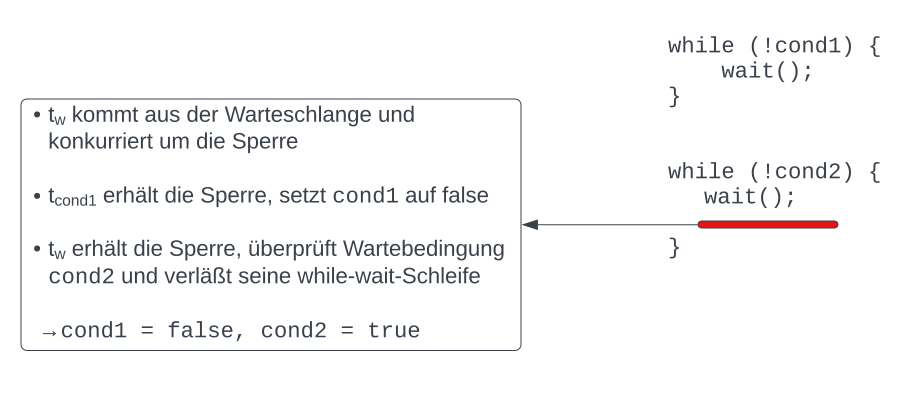
\includegraphics[scale=0.4]{chapters/Anhang/Klausuren/img/cond1cond2}
    \caption{in den rot markierten Bereich konkurriert $t_w$ um die Sperre des Objektes - wenn durch einen anderen Thread, der vor $t_w$ die Sperre erhält, \textit{cond1} auf \textit{false} gesetzt wird, stimmt die Ausgabe nicht mit der erwarteten überein. (Quelle: eigene)}
    \label{fig:cond1cond2}
\end{figure}

\noindent
Die korrekte Wartebedingung sollte lauten:

\begin{minted}[mathescape,
    linenos,
    numbersep=5pt,
    gobble=2,
    fontsize=\small,
    frame=lines,
    framesep=2mm]{java}
    public synchronized void cond1AndCond2() {
        while(!cond1 || !cond2) {
            try {
                wait();
            } catch(InterruptedException e) { }
        }
        System.out.println("cond1 and cond2:" + cond1 + " " + cond2);
    }
\end{minted}\\

Darüber hinaus müßte \code{notifyAll()} nur aufgerufen werden, wenn sowohl \code{cond1} als auch \code{cond2} auf \code{true} gesetzt sind, was leicht in den entsprechenden Methoden überprüft werden kann.
    \chapter{SS19}\label{ch:klausurss19}

\section{Aufgabe 1}

Bei der Aufgabe ist es wichtig, die Anforderungen genau zu beachten.\\
Ob eine Thread die while-wait-Schleife verlassen darf, wird von der Methode \code{tick()} gesteuert - wieviele Ticks ein Thread in der Schleife bleiben soll, wird von dem jeweiligen Thread definiert.\\
Die \code{tick()}-Methode wird von anderen Threads aufgerufen, es kann also durchaus vorkommen, dass mehrmals hintereinander
die \code{notifyAll()}-Methode aufgerufen wird - diese entfernt alle Threads aus der Warteschlange, damit die Threads ihre
Wartebedingungen erneut überprüfen können.\\
da \code{tick()} aber auch gleichzeitig einen Zähler realisieren soll, \textit{muss} es in der Methode auch eine Zählvariable geben, anhand derer die in der while-wait-Schleife enthaltenen Threads feststellen können, wie oft \code{tick()} aufgerufen wurde, um entsprechend aus der Schleife und nachfolgend der Methode herauszukommen.

\begin{figure}
    \centering
    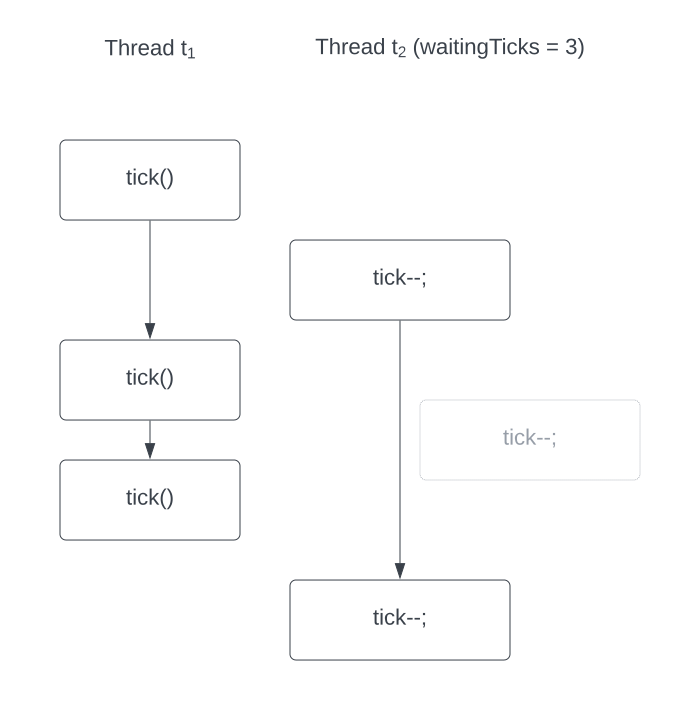
\includegraphics[scale=0.5]{chapters/Anhang/Klausuren/img/tick}
    \caption{Thread $t_1$ ruft 3 mal \texit{tick()} auf. Den Anforderungen nach müsste Thread $t_2$ danach aus der while-wait-Schleife herauskommen, erhält aber nicht die Sperre auf das Objekt von LogicalTime, um seinen eigenen Zähler rechtzeitig zu erniedrigen, bevor $t_1$ erneut \textit{tick()} aufruft. (Quelle: eigene)}
    \label{fig:tick}
\end{figure}

\section{Aufgabe 6}
Auch hier gilt, dass die Aufgabenstellung aufmerksam zu lesen ist.\\
Der Kreis soll erst ausgefüllt werden, wenn die Maustaste gelöst wird.

\begin{minted}[mathescape,
    linenos,
    numbersep=5pt,
    gobble=2,
    frame=lines,
    framesep=2mm]{java}
    private void mousePressed(double x, double y) {
        c = new Circle();
        c.setCenterX(x);
        c.setCenterY(y);
        c.setStroke(Color.RED);
        c.setFill(null); // oder Color.TRANSPARENT
        c.setRadius(RADIUS);
        graphicsPane.getChildren().add(c);
    }

    private void mouseReleased() {
        c.setFill(Color.RED);
        c = null;
    }
\end{minted}

\section{Aufgabe 8}

In der Abbildung \ref{fig:batchmodus} ist links der sequentielle Modus dargestellt, bei dem nach dem Senden einer Nachricht auf die Antwort des Servers gewartet wird, bevor eine neue Nachricht geschickt wird.
Dies wird i.d.R. verwendet, wenn das Senden einer neuen Nachricht abhängig ist von einem Ergebnis, die über die Server-Antwort übermittelt wird, oder wenn mit dem Server interagiert wird (Request abhängig vom Response).\\
Der Batch-Modus auf der rechten Seite der gleichen Abbildung ist schneller, da zwischen dem Senden von Nachrichten nicht auf Antworten gewartet werden müssen. \\
Erst nach dem Senden eine Batches von Nachrichten werden die dem Client zur Verfügung stehenden Antworten ausgelesen.\\

\noindent
In dieser Form des Batch-Modus besteht allerdings die Gefahr, dass es zu Verklemmungen kommt:
\begin{itemize}
    \item Bei dem Client kommen viele Nachrichten an, während er noch sendet.
    \item Die ankommenden Nachrichten für den Client werden gepuffert, bis sie ausgelesen werden (TCP- / OS-seitig).
    \item Läuft der Puffer voll, sorgt die Flusskontrolle (TCP) dafür, dass dem Sender mitgeteilt wird, dass keine Nachrichten mehr empfangen werden können, der Server sendet nicht mehr.
    \item Die zu sendenden Nachrichten des Servers werden in einen Puffer geschrieben.
    \item Der Sende-Puffer des Senders läuft voll.
    \item Bei dem nächsten Sende-Aufruf blockiert der Server, empfangene Nachrichten landen im Empfangspuffer
    \item Der Empfangspuffer des Servers läuft voll, der Client buffert die zu sendenden Nachrichten.
    \item Beide Anwendungen blockieren.
\end{itemize}

\\noindent
Um dieses Problem beim Batch-Modus zu umgehen, werden für das Senden und Empfangen zwei Threads auf Client-Seite erstellt: Ein Thread sendet, ein Thread empfängt. \\
Dadurch kann von dem Client immer wieder sein Empfangspuffer geleert werden, der Server wird beim Senden nicht blockiert.

\begin{figure}
    \centering
    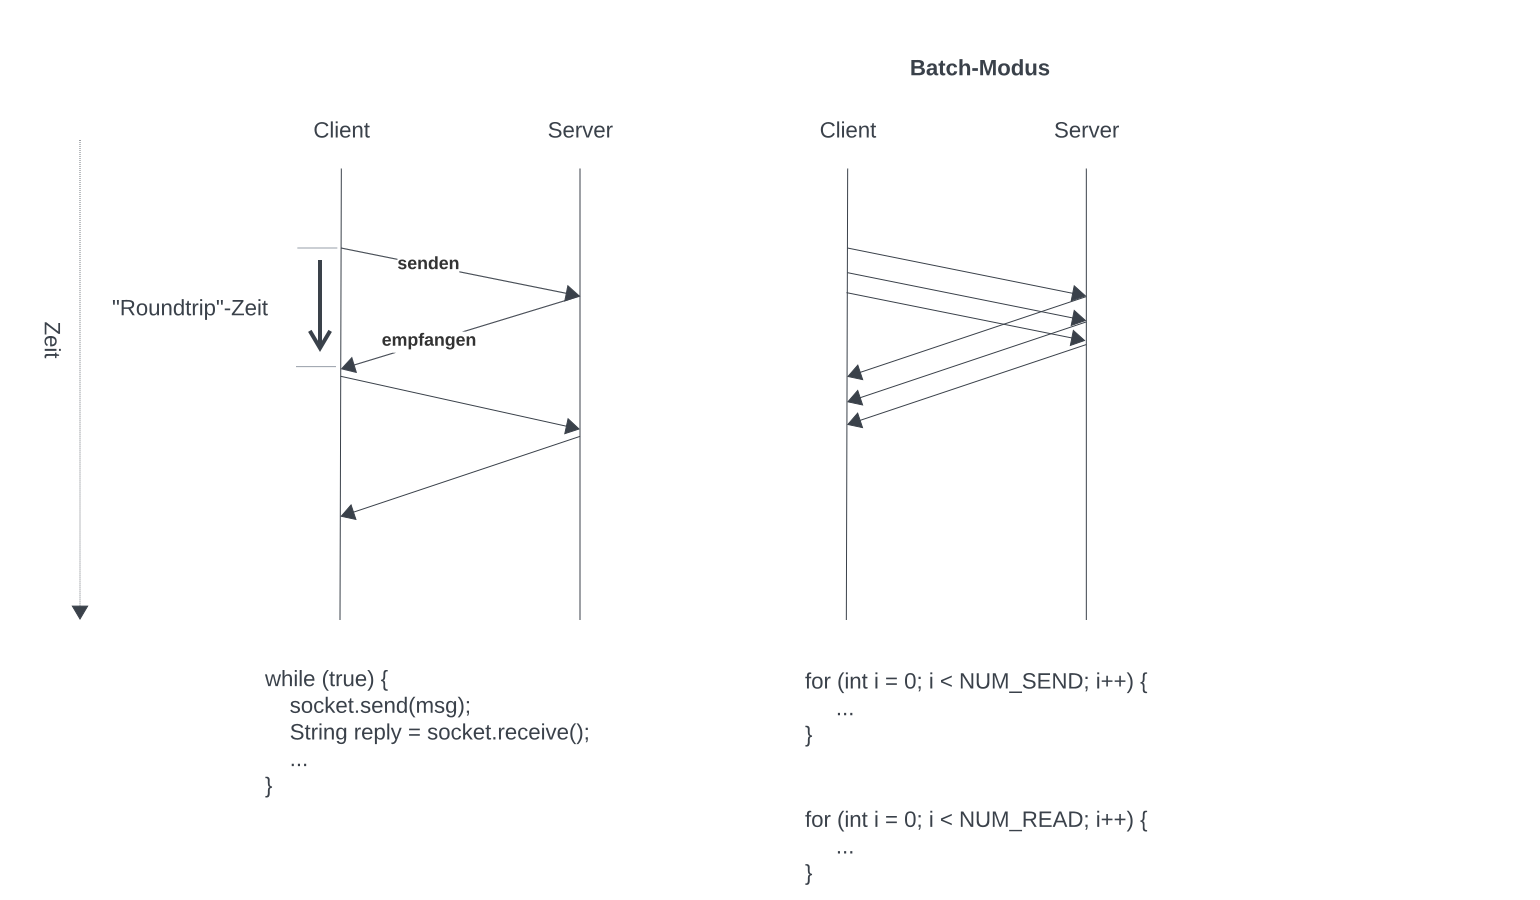
\includegraphics[scale=0.4]{chapters/Anhang/Klausuren/img/batchmodus}
    \caption{Vereinfachte Darstellung sequentieller Kommunikation und Batch-Modus (Quelle: eigene)}
    \label{fig:batchmodus}
\end{figure}
    
\begin{appendices}
    \input{chapters/Anhang/Zusatzaufgaben/index}
    \input{chapters/Anhang/Klausuren/ws13}
    \input{chapters/Anhang/Klausuren/ws15-16}
    \input{chapters/Anhang/Klausuren/ws16-17}
    \input{chapters/Anhang/Klausuren/ss19}
    \input{chapters/Anhang/Präsenzphase/index}

\end{appendices}


\end{appendices}

    \chapter{WS13}\label{ch:klausurws13}

\section{Aufgabe 1}
\subsection{Lösungsvorschlag}


\begin{minted}[mathescape,
    linenos,
    numbersep=5pt,
    gobble=2,
    fontsize=\small,
    frame=lines,
    framesep=2mm]{java}
    class Zahlenschloss {

        private int[] kombination;

        private int[] state;

        private boolean opened = false;

        public Zahlenschloss(int[] kombination) {
            this.kombination = kombination;
            this.state = new int[kombination.length];
        }

        public int anzahlRaedchen() {
            return kombination.length;
        }

        public synchronized int lesen(int radnummer) {
            return state[radnummer];
        }

        public synchronized void drehen(int radnummer, int zahl) {

            state[radnummer] = zahl;
            opened = true;
            for (int i = 0; i < anzahlRaedchen(); i++) {
                if (lesen(i) != kombination[i]) {
                    opened = false;
                    break;
                }
            }

            if (opened) {
                this.notify();
            }
        }

        public synchronized void warten() {

            while (!opened) {
                try {
                    this.wait();
                } catch (InterruptedException ignored) {}
            }
        }
    }
\end{minted}\\


\subsection{Anmerkung und Ergänzungen}

\begin{itemize}
    \item Es wird eine Wartebedingung benötigt, und zwar für die Methode \code{warten()}; ankommende Threads werden
    in die Warteschlange des Zahlenschloss-Objektes geschickt, wenn \code{opened} auf false gesetzt ist, ansonsten
    verlassen diese direkt die Methode wieder.\\
    Die Methode \code{drehen} benötigt keine separate Wartebedingung.
    Es reicht aus, sicherzustellen, dass das Zahlenschloss nicht gleichzeitig von anderen Threads benutzt werden kann:
    Die Methode \code{drehen} ist hierfür synchronisiert, damit das Zahlenschloss {insg.} immer nur eine Zustandsänderung
    erfährt - es sind andere Implementierungen möglich, in denen das Zahlenschloss dann von mehreren Threads gleichzeitig
    genutzt werden darf, wenn sich die Zugriffe anhand der ``Ziel``-\code{radnummer} unterscheiden, {bspw.} durch Mutex-Semaphore,
    die pro Radnummer verwendet werden\footnote{
        der gleichzeitige Zugriff auf unterschiedliche Arrays-Indizes ist erlaubt, s. `´17.4.1. Shared Variables``: \url{https://docs.oracle.com/javase/specs/jls/se21/html/jls-17.html#jls-1.4.1} - abgerufen 14.2.2024
    }.
    \item Es gibt nur eine Wartebedingung, von daher sollte \code{notify()} genügen.\\
    Wenn wir allerdings davon ausgehen, dass mehrere Threads über die Methode \code{warten()} in die Warteschlange des Objektes eingereiht worden sind,  sollte \code{notifyAll()} verwendet werden (siehe hierzu auch Abschnitt \ref{subsec:notifyAll}).
    Dennoch ist nicht garantiert, dass auch alle Threads aus der Warteschlange gelangen, denn es kann sein, dass ein anderer Thread die Methode \code{drehen()} betritt, dort die
    Zahlenkombination ändert und \code{opened} wieder auf \code{false} gesetzt wird. \\
    Ein anderer Thread, der nun in  \code{warten()} an die Reihe kommt, überprüft die Wartebedingung, und wird wieder in die Warteschlange eingereiht.
    Es ist also durchaus möglich, dass ein Thread nicht mehr aus der Methode \code{warten()} herauskommt.\\
    Dies könnte bspw. dadurch verhindert werden, dass die Threads in eine Queue gepackt werden, und in \code{drehen()} eine Wartebedingung eingefügt wird, die erst erfüllt ist,
    wenn die Queue geleert wurde oder aus ihr entnommen wurde, in der Reihenfolge, in der die Threads in die Queue eingereiht worden sind (\textit{FIFO}) (s. a. Abschnitt~\ref{subsec:readerwriterproblem}).
    \item Bei der Teilaufgabe mit der Schleife muss die komplette Schleife synchronisiert werden, was man durch ein \code{synchronized}-Statement erreicht\footnote{siehe Abschnitt~\ref{subsec:synchronizedstatement}.}
    \begin{minted}[mathescape,
        linenos,
        numbersep=5pt,
        gobble=2,
        fontsize=\small,
        frame=lines,
        framesep=2mm]{java}
        synchronized (zk) {
            for (int i = 0; i < anzahlRaedchen; i++) {
                System.out.println(zk.lesen(i));
            }
        }
    \end{minted}
    Ansonsten läuft man Gefahr, dass sich nach Auslesen der 1. Position der Wert von Position 2 geändert hat und dadurch eine
    Zahlenkombination ausgegeben wird, die es nicht gegeben hat:
    \begin{enumerate}
        \item $K\coloneqq[0, 0, 0]$
        \item Position $K_0$ wird ausgelesen und liefert $0$.
        \item Thread ändert $K_0$ zu $1$ $\implies K\coloneqq[1, 0, 0] $.
        \item Thread ändert $K_1$ zu $2$ $\implies K\coloneqq[1, 2, 0] $.
        \item Thread ändert $K_2$ zu $3$ $\implies K\coloneqq[1, 2, 3] $.
        \item Positionen $K_1$ und $K_2$ werden ausgelesen und liefern: $2, 3$
        \item Ausgabe: $0, 2, 3$ - diese Kombination hat es in dem Fall aber tatsächlich nicht gegeben.
    \end{enumerate}
\end{itemize}

\begin{tcolorbox}[colback=red!20,color=white,title=Anmerkung]
    Die Methode \code{lesen()} als \code{synchronized} zu markieren könnte man sich vlt. sparen, wenn man davon ausgeht,
    dass die Methode ohnehin in einem \code{synchronized}-Statement verwendet wird, um alle Rädchen abzulesen.\\
    Mehrere Threads können also nicht parallel auf unterschiedliche Positionen des Feldes zugreifen, wenn die Methode
    synchronisiert ist.\\
    Allerdings ist sowohl das Skript als auch das Buch recht klar, was in dieser Situation geschehen muss (s. Skript Fopt1/2, S. 9, außerdem \cite[31, Abschnitt 2.3.6]{Oec22}): Es muss (in diesem Kurs) immer \code{synchronized} verwendet werden, wenn gleichzeitig
    Daten geschrieben und gleichzeitig diese Daten gelesen werden sollen - und eine andere Implementierung, bei der die
    einzelnen Positionen ``gelocked`` sind, so dass ein gleichzeitiger Zugriff auf unterschiedliche Rädchen möglich ist, war nicht gefordert.\\
    Ggfl. würde in anderen Implementierungen der Einsatz von \code{AtomicReferenceArray}\footnote{s. \cite[157 ff.]{Oec22}
    s. ``Class AtomicReferenceArray<E>``: \url{https://docs.oracle.com/en/java/javase/21/docs/api/java.base/java/util/concurrent/atomic/AtomicReferenceArray.html} - abgerufen 15.2.2024
    } Sinn machen, aber das Lehrmaterial ist bereits sehr eindeutig bzgl. der Verwendung von \code{synchronized}.
\end{tcolorbox}



\section{Aufgabe 3}
\subsection{Lösungsvorschlag}

\subsection*{Statische Parallelität}
Statische Parallelität erlaubt es einem Server, eine \textit{fixe} Anzahl von Verbindungen gleichzeitig zu bedienen.\\
Hierbei wird ein Feld von Threads erstellt, wobei jeder Thread das \code{ServerSocket}-Objekt als Referenz übergeben bekommt.
In der \code{run()}-Methode wird dann über \code{accept()} in einer Endlosschleife auf eingehende Verbindungen gewartet, die dann so lange bedient werden, bis sich ein Client wieder abmeldet (oder eine andere Abbruchbedingung erfüllt ist, wie z.B. ein \code{SocketTimeout}).\\
Das sich ein Client abmeldet, bekommt man bspw. dadurch mit, dass \code{null} beim Lesen von einer Nachricht des Clients zurückgegeben wird (vgl. \cite[286]{Oec22}. \\
Siehe Abschnitt~\ref{sec:seqparserver} für ein Implementierungsbeispiel.



\subsection*{Dynamische Parallelität}

Bei der \textbf{Dynamischer Parallelität} erzeugt der Server für jede Verbindung einen neuen Thread, der so lange läuft, bis der Client die Verbindung wieder trennt.\\
Die Anzahl der Threads ändert sich dadurch laufend.\\
Wird die max. Anzahl erlaubter Threads nicht kontrolliert, kann es zu einer Überlastung des Server-Rechners kommen (bspw. durch einen Denial-of-Service-Angriff.)\\

\noindent
I.d.R. ist eine Mischform aus beidem geeignet, um mehrere Clients gleichzeitig bedienen zu können, und dabei nicht Gefahr zu laufen, durch dynamisches, unbegrenztes Wachstum der Anzahl der Threads überlastet zu werden.

    \chapter{WS13}\label{ch:klausurws5-16}

\section{Rechteck-Scroll (SS15 Aufgabe 2)}

Aufgabenstellung unklar.\\
Mögliche Implementierung unter \url{https://github.com/ThorstenSuckow/fopt/tree/main/src/main/java/klausurvorbereitung/foptws1516/MouseDragsSquareDemo}.

\section{Rechteck-Scroll (WS15/16 Aufgabe 1)}

Aufgabenstellung unklar.\\
Mögliche Implementierung unter \url{https://github.com/ThorstenSuckow/fopt/tree/main/src/main/java/klausurvorbereitung/foptws1516/MaxWeightDemo}.\\

\noindent
Es gibt nur eine Warteschlange für Threads in \code{use()}, es gibt keine Wartebedingung in \code{dontUse()} und damit auch keine weitere Warteschlange.\\
Es sind durch die Zugriffe auf unterschiedliche Indizes allerdings mehrere Wartebedingungen vorhanden, weshalb hab \code{notifyAll()} nutzen sollte,
sobald ein Zugriff auf ein Feld nach Aufruf von \code{dontUse} wieder möglich wird.\\
Ansonsten bestünde die Gefahr, dass bei dem Einsatz von \code{notify()} ein wartender Thread nicht geweckt wird, obwohl er weiterlaufen könnte:\\
Angenommen, das Feld $F$ hat eine Länge von $3$, das \code{maxWeight} ist mit $2$ konfiguriert.
Thread $t_1$ mit einer Laufzeit von $200\ sek$ bekommt Zugriff auf $F_0$, setzt $currentWeight$ auf $1$.\\
Thread $t_2$ mit einer Laufzeit von $1\ sek$ möchte auf $F_1$ zugreifen, setzt $currentWeight=2$ in die Warteschlange.\\
Thread $t_3$ meldet Zugriff auf $F_0$ an und gelangt in die Warteschlange.\\
Thread $t_4$ meldet Zugriff auf $F_1$ an und gelangt in die Warteschlange.\\
Thread $t_2$ ist mit der Bearbeitung von $F_1$ fertig, $currentWeight$ wird auf $1$ gesetzt, \code{notify()} wird aufgerufen.\\
Thread $t_3$ wird aus der Warteschlange geholt, kann aber nicht weiterarbeiten, da $F_0$ noch durch den länger dauernden $t_1$ blockiert ist, und kommt wieder in die Warteschlange.\\

\noindent
Offensichtlich hätte in dem Beispiel \code{notifyAll()} dazu geführt, dass auch $T_4$ seine Wartebedingung hätte überprüfen können, und hätte so Zugriff auf $F_1$ bekommen.
Stattdessen muss nun gewartet werden, bis das nächste \code{notify()} aufgerufen wird, oder ein neu ankommender Thread $F_1$ belegt.

    \chapter{WS16-17}\label{ch:klausurws16-17}

\section{Aufgabe 1}
\subsection{Lösungshinweis}

Die erste Aufgabe verdeutlicht, was bei einem \code{notifyAll()} und unsauber gesetzten Wartebedingungen passieren kann.\\
Sei folgender Quellcode gegeben:


\begin{minted}[mathescape,
    linenos,
    numbersep=5pt,
    gobble=2,
    fontsize=\small,
    frame=lines,
    framesep=2mm]{java}
    class Cond1AndCond2 {

        private boolean cond1;
        private boolean cond2;

        public synchronized void setCond1(boolean c) {
            cond1 = c;
            notifyAll();
        }

        public synchronized void setCond2(boolean c) {
            cond2 = c;
            notifyAll();
        }

        public synchronized void cond1AndCond2() {
            while(!cond1) {
                try {
                    wait();
                } catch(InterruptedException e) { }
            }

            while(!cond2) {
                try {
                    wait();
                } catch(InterruptedException e) {}
            }
            System.out.println("cond1 and cond2:" + cond1 + " " + cond2);
        }
    }
\end{minted}\\

Man sollte auf den ersten Blick meinen, dass \code{cond1} und \code{cond2} beide \code{true} sein müssen, damit die Ausgabe erfolgt.\\
Tatsächlich ist es aber so, dass es in der Methode zwei unterschiedliche Wartebedingungen gibt.\\
Die erste Wartebedingung schickt einen Thread in die Warteschlange, wenn \code{cond1 == false} gilt.\\
Setzt ein anderer Thread über \code{setCond1(true)} das Attribut entsprechend auf \code{true}, bewirkt der nachfolgende Aufruf von \code{notifyAll()}, dass alle \textit{wartenden} Threads aus der Warteschlange entfernt werden und erneut um eine Sperre des Objektes konkurrieren.\\
Erhält ein entsprechender Thread $t_w$ die Sperre auf das Objekt und kann seine \textit{while-wait-Schleife} verlassen, kann es vorkommen, dass er erneut in die Warteschlange eingereiht wird, wegen der nachfolgenden Wartebedingung \code{cond2 == false}.\\
Angenommen, ein weiterer Thread ruft nun \code{setCond2(true)} auf, und $t_w$ kommt aus der Warteschlange und konkurriert erneut und um die Sperre des Objektes, dann kann es vorkommen, das ein anderer Thread zunächst die Sperre erhält, \code{cond1} wieder auf \code{false} setzt, dann erhält $t_w$ die Sperre, überprüft die Wartebedingung \code{cond2 == false}.\\
Wegen \code{cond2} gelangt er aus der \textit{while-wait-Schleife} und die Ausgabe erfolgt - da zwischenzeitlich \code{cond1} wieder auf \code{false} gesetzt wurde, ist die erwartete Ausgabe nicht \code{true true}, sondern \code{false true} (s. Abbildung \ref{fig:cond1cond2}).\\

\begin{figure}
    \centering
    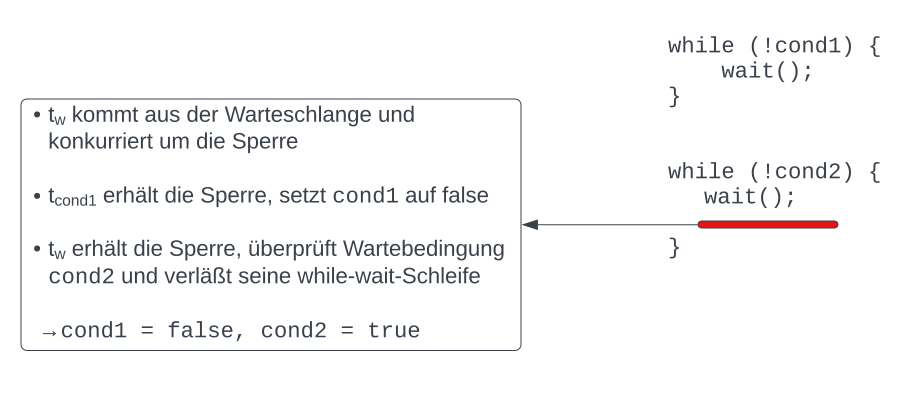
\includegraphics[scale=0.4]{chapters/Anhang/Klausuren/img/cond1cond2}
    \caption{in den rot markierten Bereich konkurriert $t_w$ um die Sperre des Objektes - wenn durch einen anderen Thread, der vor $t_w$ die Sperre erhält, \textit{cond1} auf \textit{false} gesetzt wird, stimmt die Ausgabe nicht mit der erwarteten überein. (Quelle: eigene)}
    \label{fig:cond1cond2}
\end{figure}

\noindent
Die korrekte Wartebedingung sollte lauten:

\begin{minted}[mathescape,
    linenos,
    numbersep=5pt,
    gobble=2,
    fontsize=\small,
    frame=lines,
    framesep=2mm]{java}
    public synchronized void cond1AndCond2() {
        while(!cond1 || !cond2) {
            try {
                wait();
            } catch(InterruptedException e) { }
        }
        System.out.println("cond1 and cond2:" + cond1 + " " + cond2);
    }
\end{minted}\\

Darüber hinaus müßte \code{notifyAll()} nur aufgerufen werden, wenn sowohl \code{cond1} als auch \code{cond2} auf \code{true} gesetzt sind, was leicht in den entsprechenden Methoden überprüft werden kann.
    \chapter{SS19}\label{ch:klausurss19}

\section{Aufgabe 1}

Bei der Aufgabe ist es wichtig, die Anforderungen genau zu beachten.\\
Ob eine Thread die while-wait-Schleife verlassen darf, wird von der Methode \code{tick()} gesteuert - wieviele Ticks ein Thread in der Schleife bleiben soll, wird von dem jeweiligen Thread definiert.\\
Die \code{tick()}-Methode wird von anderen Threads aufgerufen, es kann also durchaus vorkommen, dass mehrmals hintereinander
die \code{notifyAll()}-Methode aufgerufen wird - diese entfernt alle Threads aus der Warteschlange, damit die Threads ihre
Wartebedingungen erneut überprüfen können.\\
da \code{tick()} aber auch gleichzeitig einen Zähler realisieren soll, \textit{muss} es in der Methode auch eine Zählvariable geben, anhand derer die in der while-wait-Schleife enthaltenen Threads feststellen können, wie oft \code{tick()} aufgerufen wurde, um entsprechend aus der Schleife und nachfolgend der Methode herauszukommen.

\begin{figure}
    \centering
    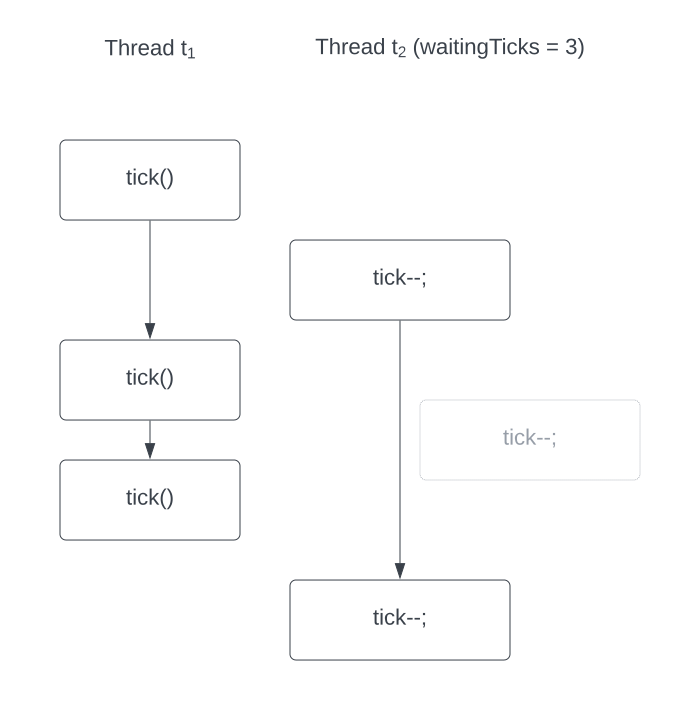
\includegraphics[scale=0.5]{chapters/Anhang/Klausuren/img/tick}
    \caption{Thread $t_1$ ruft 3 mal \texit{tick()} auf. Den Anforderungen nach müsste Thread $t_2$ danach aus der while-wait-Schleife herauskommen, erhält aber nicht die Sperre auf das Objekt von LogicalTime, um seinen eigenen Zähler rechtzeitig zu erniedrigen, bevor $t_1$ erneut \textit{tick()} aufruft. (Quelle: eigene)}
    \label{fig:tick}
\end{figure}

\section{Aufgabe 6}
Auch hier gilt, dass die Aufgabenstellung aufmerksam zu lesen ist.\\
Der Kreis soll erst ausgefüllt werden, wenn die Maustaste gelöst wird.

\begin{minted}[mathescape,
    linenos,
    numbersep=5pt,
    gobble=2,
    frame=lines,
    framesep=2mm]{java}
    private void mousePressed(double x, double y) {
        c = new Circle();
        c.setCenterX(x);
        c.setCenterY(y);
        c.setStroke(Color.RED);
        c.setFill(null); // oder Color.TRANSPARENT
        c.setRadius(RADIUS);
        graphicsPane.getChildren().add(c);
    }

    private void mouseReleased() {
        c.setFill(Color.RED);
        c = null;
    }
\end{minted}

\section{Aufgabe 8}

In der Abbildung \ref{fig:batchmodus} ist links der sequentielle Modus dargestellt, bei dem nach dem Senden einer Nachricht auf die Antwort des Servers gewartet wird, bevor eine neue Nachricht geschickt wird.
Dies wird i.d.R. verwendet, wenn das Senden einer neuen Nachricht abhängig ist von einem Ergebnis, die über die Server-Antwort übermittelt wird, oder wenn mit dem Server interagiert wird (Request abhängig vom Response).\\
Der Batch-Modus auf der rechten Seite der gleichen Abbildung ist schneller, da zwischen dem Senden von Nachrichten nicht auf Antworten gewartet werden müssen. \\
Erst nach dem Senden eine Batches von Nachrichten werden die dem Client zur Verfügung stehenden Antworten ausgelesen.\\

\noindent
In dieser Form des Batch-Modus besteht allerdings die Gefahr, dass es zu Verklemmungen kommt:
\begin{itemize}
    \item Bei dem Client kommen viele Nachrichten an, während er noch sendet.
    \item Die ankommenden Nachrichten für den Client werden gepuffert, bis sie ausgelesen werden (TCP- / OS-seitig).
    \item Läuft der Puffer voll, sorgt die Flusskontrolle (TCP) dafür, dass dem Sender mitgeteilt wird, dass keine Nachrichten mehr empfangen werden können, der Server sendet nicht mehr.
    \item Die zu sendenden Nachrichten des Servers werden in einen Puffer geschrieben.
    \item Der Sende-Puffer des Senders läuft voll.
    \item Bei dem nächsten Sende-Aufruf blockiert der Server, empfangene Nachrichten landen im Empfangspuffer
    \item Der Empfangspuffer des Servers läuft voll, der Client buffert die zu sendenden Nachrichten.
    \item Beide Anwendungen blockieren.
\end{itemize}

\\noindent
Um dieses Problem beim Batch-Modus zu umgehen, werden für das Senden und Empfangen zwei Threads auf Client-Seite erstellt: Ein Thread sendet, ein Thread empfängt. \\
Dadurch kann von dem Client immer wieder sein Empfangspuffer geleert werden, der Server wird beim Senden nicht blockiert.

\begin{figure}
    \centering
    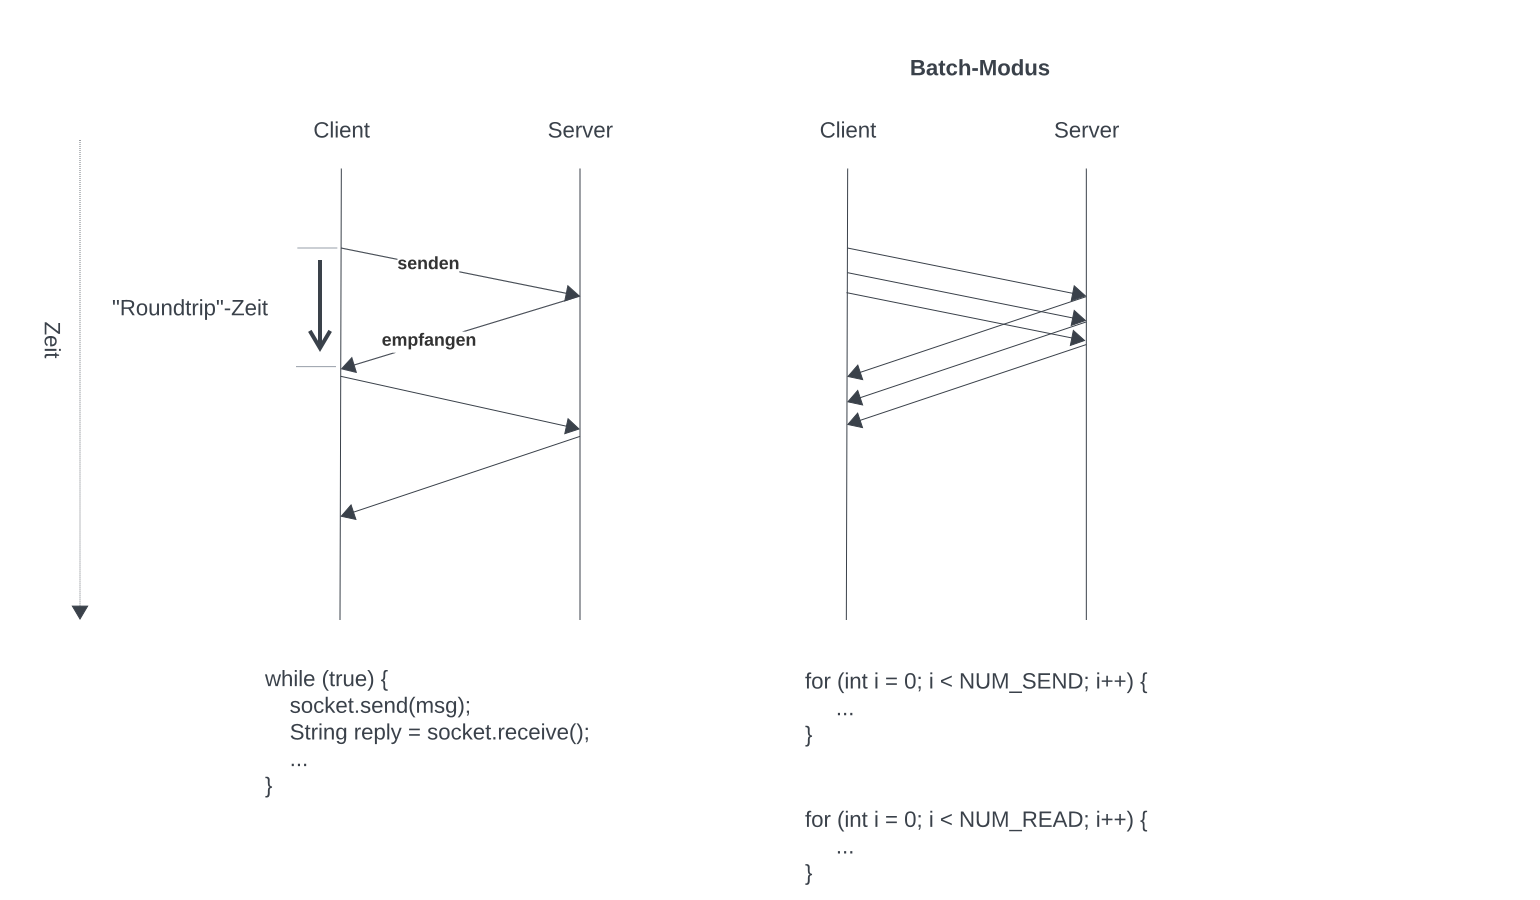
\includegraphics[scale=0.4]{chapters/Anhang/Klausuren/img/batchmodus}
    \caption{Vereinfachte Darstellung sequentieller Kommunikation und Batch-Modus (Quelle: eigene)}
    \label{fig:batchmodus}
\end{figure}
    
\begin{appendices}
    
\begin{appendices}
    \input{chapters/Anhang/Zusatzaufgaben/index}
    \input{chapters/Anhang/Klausuren/ws13}
    \input{chapters/Anhang/Klausuren/ws15-16}
    \input{chapters/Anhang/Klausuren/ws16-17}
    \input{chapters/Anhang/Klausuren/ss19}
    \input{chapters/Anhang/Präsenzphase/index}

\end{appendices}

    \chapter{WS13}\label{ch:klausurws13}

\section{Aufgabe 1}
\subsection{Lösungsvorschlag}


\begin{minted}[mathescape,
    linenos,
    numbersep=5pt,
    gobble=2,
    fontsize=\small,
    frame=lines,
    framesep=2mm]{java}
    class Zahlenschloss {

        private int[] kombination;

        private int[] state;

        private boolean opened = false;

        public Zahlenschloss(int[] kombination) {
            this.kombination = kombination;
            this.state = new int[kombination.length];
        }

        public int anzahlRaedchen() {
            return kombination.length;
        }

        public synchronized int lesen(int radnummer) {
            return state[radnummer];
        }

        public synchronized void drehen(int radnummer, int zahl) {

            state[radnummer] = zahl;
            opened = true;
            for (int i = 0; i < anzahlRaedchen(); i++) {
                if (lesen(i) != kombination[i]) {
                    opened = false;
                    break;
                }
            }

            if (opened) {
                this.notify();
            }
        }

        public synchronized void warten() {

            while (!opened) {
                try {
                    this.wait();
                } catch (InterruptedException ignored) {}
            }
        }
    }
\end{minted}\\


\subsection{Anmerkung und Ergänzungen}

\begin{itemize}
    \item Es wird eine Wartebedingung benötigt, und zwar für die Methode \code{warten()}; ankommende Threads werden
    in die Warteschlange des Zahlenschloss-Objektes geschickt, wenn \code{opened} auf false gesetzt ist, ansonsten
    verlassen diese direkt die Methode wieder.\\
    Die Methode \code{drehen} benötigt keine separate Wartebedingung.
    Es reicht aus, sicherzustellen, dass das Zahlenschloss nicht gleichzeitig von anderen Threads benutzt werden kann:
    Die Methode \code{drehen} ist hierfür synchronisiert, damit das Zahlenschloss {insg.} immer nur eine Zustandsänderung
    erfährt - es sind andere Implementierungen möglich, in denen das Zahlenschloss dann von mehreren Threads gleichzeitig
    genutzt werden darf, wenn sich die Zugriffe anhand der ``Ziel``-\code{radnummer} unterscheiden, {bspw.} durch Mutex-Semaphore,
    die pro Radnummer verwendet werden\footnote{
        der gleichzeitige Zugriff auf unterschiedliche Arrays-Indizes ist erlaubt, s. `´17.4.1. Shared Variables``: \url{https://docs.oracle.com/javase/specs/jls/se21/html/jls-17.html#jls-1.4.1} - abgerufen 14.2.2024
    }.
    \item Es gibt nur eine Wartebedingung, von daher sollte \code{notify()} genügen.\\
    Wenn wir allerdings davon ausgehen, dass mehrere Threads über die Methode \code{warten()} in die Warteschlange des Objektes eingereiht worden sind,  sollte \code{notifyAll()} verwendet werden (siehe hierzu auch Abschnitt \ref{subsec:notifyAll}).
    Dennoch ist nicht garantiert, dass auch alle Threads aus der Warteschlange gelangen, denn es kann sein, dass ein anderer Thread die Methode \code{drehen()} betritt, dort die
    Zahlenkombination ändert und \code{opened} wieder auf \code{false} gesetzt wird. \\
    Ein anderer Thread, der nun in  \code{warten()} an die Reihe kommt, überprüft die Wartebedingung, und wird wieder in die Warteschlange eingereiht.
    Es ist also durchaus möglich, dass ein Thread nicht mehr aus der Methode \code{warten()} herauskommt.\\
    Dies könnte bspw. dadurch verhindert werden, dass die Threads in eine Queue gepackt werden, und in \code{drehen()} eine Wartebedingung eingefügt wird, die erst erfüllt ist,
    wenn die Queue geleert wurde oder aus ihr entnommen wurde, in der Reihenfolge, in der die Threads in die Queue eingereiht worden sind (\textit{FIFO}) (s. a. Abschnitt~\ref{subsec:readerwriterproblem}).
    \item Bei der Teilaufgabe mit der Schleife muss die komplette Schleife synchronisiert werden, was man durch ein \code{synchronized}-Statement erreicht\footnote{siehe Abschnitt~\ref{subsec:synchronizedstatement}.}
    \begin{minted}[mathescape,
        linenos,
        numbersep=5pt,
        gobble=2,
        fontsize=\small,
        frame=lines,
        framesep=2mm]{java}
        synchronized (zk) {
            for (int i = 0; i < anzahlRaedchen; i++) {
                System.out.println(zk.lesen(i));
            }
        }
    \end{minted}
    Ansonsten läuft man Gefahr, dass sich nach Auslesen der 1. Position der Wert von Position 2 geändert hat und dadurch eine
    Zahlenkombination ausgegeben wird, die es nicht gegeben hat:
    \begin{enumerate}
        \item $K\coloneqq[0, 0, 0]$
        \item Position $K_0$ wird ausgelesen und liefert $0$.
        \item Thread ändert $K_0$ zu $1$ $\implies K\coloneqq[1, 0, 0] $.
        \item Thread ändert $K_1$ zu $2$ $\implies K\coloneqq[1, 2, 0] $.
        \item Thread ändert $K_2$ zu $3$ $\implies K\coloneqq[1, 2, 3] $.
        \item Positionen $K_1$ und $K_2$ werden ausgelesen und liefern: $2, 3$
        \item Ausgabe: $0, 2, 3$ - diese Kombination hat es in dem Fall aber tatsächlich nicht gegeben.
    \end{enumerate}
\end{itemize}

\begin{tcolorbox}[colback=red!20,color=white,title=Anmerkung]
    Die Methode \code{lesen()} als \code{synchronized} zu markieren könnte man sich vlt. sparen, wenn man davon ausgeht,
    dass die Methode ohnehin in einem \code{synchronized}-Statement verwendet wird, um alle Rädchen abzulesen.\\
    Mehrere Threads können also nicht parallel auf unterschiedliche Positionen des Feldes zugreifen, wenn die Methode
    synchronisiert ist.\\
    Allerdings ist sowohl das Skript als auch das Buch recht klar, was in dieser Situation geschehen muss (s. Skript Fopt1/2, S. 9, außerdem \cite[31, Abschnitt 2.3.6]{Oec22}): Es muss (in diesem Kurs) immer \code{synchronized} verwendet werden, wenn gleichzeitig
    Daten geschrieben und gleichzeitig diese Daten gelesen werden sollen - und eine andere Implementierung, bei der die
    einzelnen Positionen ``gelocked`` sind, so dass ein gleichzeitiger Zugriff auf unterschiedliche Rädchen möglich ist, war nicht gefordert.\\
    Ggfl. würde in anderen Implementierungen der Einsatz von \code{AtomicReferenceArray}\footnote{s. \cite[157 ff.]{Oec22}
    s. ``Class AtomicReferenceArray<E>``: \url{https://docs.oracle.com/en/java/javase/21/docs/api/java.base/java/util/concurrent/atomic/AtomicReferenceArray.html} - abgerufen 15.2.2024
    } Sinn machen, aber das Lehrmaterial ist bereits sehr eindeutig bzgl. der Verwendung von \code{synchronized}.
\end{tcolorbox}



\section{Aufgabe 3}
\subsection{Lösungsvorschlag}

\subsection*{Statische Parallelität}
Statische Parallelität erlaubt es einem Server, eine \textit{fixe} Anzahl von Verbindungen gleichzeitig zu bedienen.\\
Hierbei wird ein Feld von Threads erstellt, wobei jeder Thread das \code{ServerSocket}-Objekt als Referenz übergeben bekommt.
In der \code{run()}-Methode wird dann über \code{accept()} in einer Endlosschleife auf eingehende Verbindungen gewartet, die dann so lange bedient werden, bis sich ein Client wieder abmeldet (oder eine andere Abbruchbedingung erfüllt ist, wie z.B. ein \code{SocketTimeout}).\\
Das sich ein Client abmeldet, bekommt man bspw. dadurch mit, dass \code{null} beim Lesen von einer Nachricht des Clients zurückgegeben wird (vgl. \cite[286]{Oec22}. \\
Siehe Abschnitt~\ref{sec:seqparserver} für ein Implementierungsbeispiel.



\subsection*{Dynamische Parallelität}

Bei der \textbf{Dynamischer Parallelität} erzeugt der Server für jede Verbindung einen neuen Thread, der so lange läuft, bis der Client die Verbindung wieder trennt.\\
Die Anzahl der Threads ändert sich dadurch laufend.\\
Wird die max. Anzahl erlaubter Threads nicht kontrolliert, kann es zu einer Überlastung des Server-Rechners kommen (bspw. durch einen Denial-of-Service-Angriff.)\\

\noindent
I.d.R. ist eine Mischform aus beidem geeignet, um mehrere Clients gleichzeitig bedienen zu können, und dabei nicht Gefahr zu laufen, durch dynamisches, unbegrenztes Wachstum der Anzahl der Threads überlastet zu werden.

    \chapter{WS13}\label{ch:klausurws5-16}

\section{Rechteck-Scroll (SS15 Aufgabe 2)}

Aufgabenstellung unklar.\\
Mögliche Implementierung unter \url{https://github.com/ThorstenSuckow/fopt/tree/main/src/main/java/klausurvorbereitung/foptws1516/MouseDragsSquareDemo}.

\section{Rechteck-Scroll (WS15/16 Aufgabe 1)}

Aufgabenstellung unklar.\\
Mögliche Implementierung unter \url{https://github.com/ThorstenSuckow/fopt/tree/main/src/main/java/klausurvorbereitung/foptws1516/MaxWeightDemo}.\\

\noindent
Es gibt nur eine Warteschlange für Threads in \code{use()}, es gibt keine Wartebedingung in \code{dontUse()} und damit auch keine weitere Warteschlange.\\
Es sind durch die Zugriffe auf unterschiedliche Indizes allerdings mehrere Wartebedingungen vorhanden, weshalb hab \code{notifyAll()} nutzen sollte,
sobald ein Zugriff auf ein Feld nach Aufruf von \code{dontUse} wieder möglich wird.\\
Ansonsten bestünde die Gefahr, dass bei dem Einsatz von \code{notify()} ein wartender Thread nicht geweckt wird, obwohl er weiterlaufen könnte:\\
Angenommen, das Feld $F$ hat eine Länge von $3$, das \code{maxWeight} ist mit $2$ konfiguriert.
Thread $t_1$ mit einer Laufzeit von $200\ sek$ bekommt Zugriff auf $F_0$, setzt $currentWeight$ auf $1$.\\
Thread $t_2$ mit einer Laufzeit von $1\ sek$ möchte auf $F_1$ zugreifen, setzt $currentWeight=2$ in die Warteschlange.\\
Thread $t_3$ meldet Zugriff auf $F_0$ an und gelangt in die Warteschlange.\\
Thread $t_4$ meldet Zugriff auf $F_1$ an und gelangt in die Warteschlange.\\
Thread $t_2$ ist mit der Bearbeitung von $F_1$ fertig, $currentWeight$ wird auf $1$ gesetzt, \code{notify()} wird aufgerufen.\\
Thread $t_3$ wird aus der Warteschlange geholt, kann aber nicht weiterarbeiten, da $F_0$ noch durch den länger dauernden $t_1$ blockiert ist, und kommt wieder in die Warteschlange.\\

\noindent
Offensichtlich hätte in dem Beispiel \code{notifyAll()} dazu geführt, dass auch $T_4$ seine Wartebedingung hätte überprüfen können, und hätte so Zugriff auf $F_1$ bekommen.
Stattdessen muss nun gewartet werden, bis das nächste \code{notify()} aufgerufen wird, oder ein neu ankommender Thread $F_1$ belegt.

    \chapter{WS16-17}\label{ch:klausurws16-17}

\section{Aufgabe 1}
\subsection{Lösungshinweis}

Die erste Aufgabe verdeutlicht, was bei einem \code{notifyAll()} und unsauber gesetzten Wartebedingungen passieren kann.\\
Sei folgender Quellcode gegeben:


\begin{minted}[mathescape,
    linenos,
    numbersep=5pt,
    gobble=2,
    fontsize=\small,
    frame=lines,
    framesep=2mm]{java}
    class Cond1AndCond2 {

        private boolean cond1;
        private boolean cond2;

        public synchronized void setCond1(boolean c) {
            cond1 = c;
            notifyAll();
        }

        public synchronized void setCond2(boolean c) {
            cond2 = c;
            notifyAll();
        }

        public synchronized void cond1AndCond2() {
            while(!cond1) {
                try {
                    wait();
                } catch(InterruptedException e) { }
            }

            while(!cond2) {
                try {
                    wait();
                } catch(InterruptedException e) {}
            }
            System.out.println("cond1 and cond2:" + cond1 + " " + cond2);
        }
    }
\end{minted}\\

Man sollte auf den ersten Blick meinen, dass \code{cond1} und \code{cond2} beide \code{true} sein müssen, damit die Ausgabe erfolgt.\\
Tatsächlich ist es aber so, dass es in der Methode zwei unterschiedliche Wartebedingungen gibt.\\
Die erste Wartebedingung schickt einen Thread in die Warteschlange, wenn \code{cond1 == false} gilt.\\
Setzt ein anderer Thread über \code{setCond1(true)} das Attribut entsprechend auf \code{true}, bewirkt der nachfolgende Aufruf von \code{notifyAll()}, dass alle \textit{wartenden} Threads aus der Warteschlange entfernt werden und erneut um eine Sperre des Objektes konkurrieren.\\
Erhält ein entsprechender Thread $t_w$ die Sperre auf das Objekt und kann seine \textit{while-wait-Schleife} verlassen, kann es vorkommen, dass er erneut in die Warteschlange eingereiht wird, wegen der nachfolgenden Wartebedingung \code{cond2 == false}.\\
Angenommen, ein weiterer Thread ruft nun \code{setCond2(true)} auf, und $t_w$ kommt aus der Warteschlange und konkurriert erneut und um die Sperre des Objektes, dann kann es vorkommen, das ein anderer Thread zunächst die Sperre erhält, \code{cond1} wieder auf \code{false} setzt, dann erhält $t_w$ die Sperre, überprüft die Wartebedingung \code{cond2 == false}.\\
Wegen \code{cond2} gelangt er aus der \textit{while-wait-Schleife} und die Ausgabe erfolgt - da zwischenzeitlich \code{cond1} wieder auf \code{false} gesetzt wurde, ist die erwartete Ausgabe nicht \code{true true}, sondern \code{false true} (s. Abbildung \ref{fig:cond1cond2}).\\

\begin{figure}
    \centering
    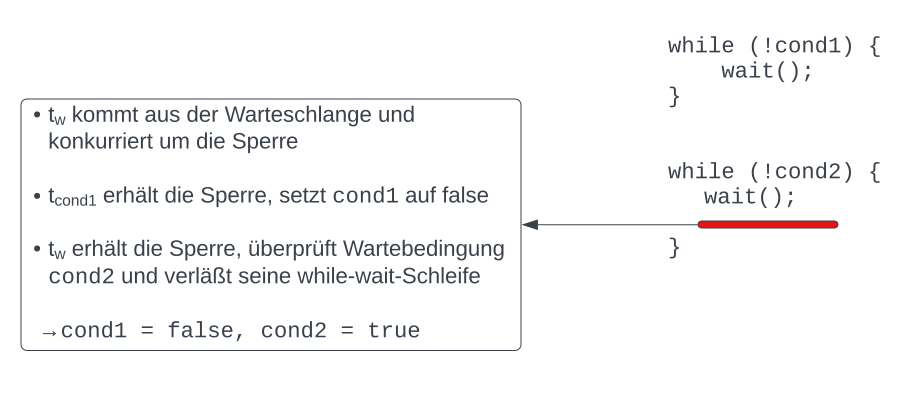
\includegraphics[scale=0.4]{chapters/Anhang/Klausuren/img/cond1cond2}
    \caption{in den rot markierten Bereich konkurriert $t_w$ um die Sperre des Objektes - wenn durch einen anderen Thread, der vor $t_w$ die Sperre erhält, \textit{cond1} auf \textit{false} gesetzt wird, stimmt die Ausgabe nicht mit der erwarteten überein. (Quelle: eigene)}
    \label{fig:cond1cond2}
\end{figure}

\noindent
Die korrekte Wartebedingung sollte lauten:

\begin{minted}[mathescape,
    linenos,
    numbersep=5pt,
    gobble=2,
    fontsize=\small,
    frame=lines,
    framesep=2mm]{java}
    public synchronized void cond1AndCond2() {
        while(!cond1 || !cond2) {
            try {
                wait();
            } catch(InterruptedException e) { }
        }
        System.out.println("cond1 and cond2:" + cond1 + " " + cond2);
    }
\end{minted}\\

Darüber hinaus müßte \code{notifyAll()} nur aufgerufen werden, wenn sowohl \code{cond1} als auch \code{cond2} auf \code{true} gesetzt sind, was leicht in den entsprechenden Methoden überprüft werden kann.
    \chapter{SS19}\label{ch:klausurss19}

\section{Aufgabe 1}

Bei der Aufgabe ist es wichtig, die Anforderungen genau zu beachten.\\
Ob eine Thread die while-wait-Schleife verlassen darf, wird von der Methode \code{tick()} gesteuert - wieviele Ticks ein Thread in der Schleife bleiben soll, wird von dem jeweiligen Thread definiert.\\
Die \code{tick()}-Methode wird von anderen Threads aufgerufen, es kann also durchaus vorkommen, dass mehrmals hintereinander
die \code{notifyAll()}-Methode aufgerufen wird - diese entfernt alle Threads aus der Warteschlange, damit die Threads ihre
Wartebedingungen erneut überprüfen können.\\
da \code{tick()} aber auch gleichzeitig einen Zähler realisieren soll, \textit{muss} es in der Methode auch eine Zählvariable geben, anhand derer die in der while-wait-Schleife enthaltenen Threads feststellen können, wie oft \code{tick()} aufgerufen wurde, um entsprechend aus der Schleife und nachfolgend der Methode herauszukommen.

\begin{figure}
    \centering
    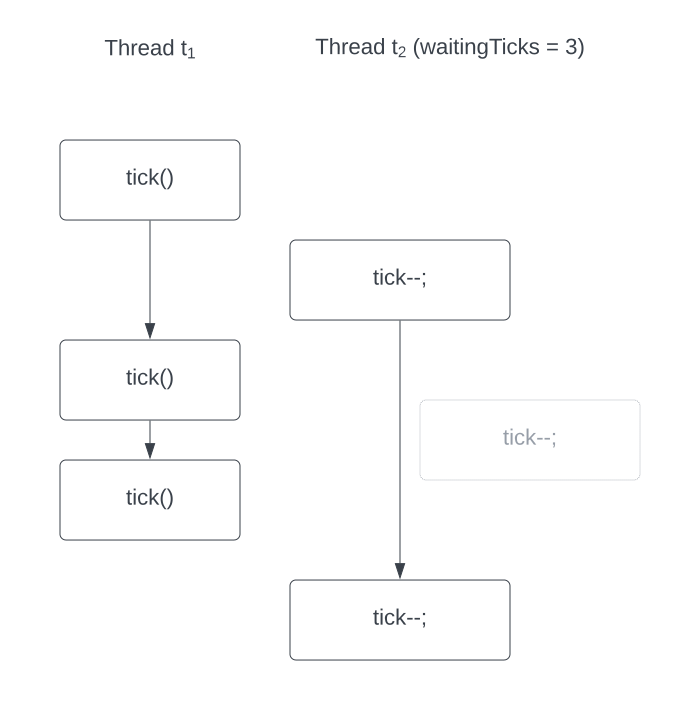
\includegraphics[scale=0.5]{chapters/Anhang/Klausuren/img/tick}
    \caption{Thread $t_1$ ruft 3 mal \texit{tick()} auf. Den Anforderungen nach müsste Thread $t_2$ danach aus der while-wait-Schleife herauskommen, erhält aber nicht die Sperre auf das Objekt von LogicalTime, um seinen eigenen Zähler rechtzeitig zu erniedrigen, bevor $t_1$ erneut \textit{tick()} aufruft. (Quelle: eigene)}
    \label{fig:tick}
\end{figure}

\section{Aufgabe 6}
Auch hier gilt, dass die Aufgabenstellung aufmerksam zu lesen ist.\\
Der Kreis soll erst ausgefüllt werden, wenn die Maustaste gelöst wird.

\begin{minted}[mathescape,
    linenos,
    numbersep=5pt,
    gobble=2,
    frame=lines,
    framesep=2mm]{java}
    private void mousePressed(double x, double y) {
        c = new Circle();
        c.setCenterX(x);
        c.setCenterY(y);
        c.setStroke(Color.RED);
        c.setFill(null); // oder Color.TRANSPARENT
        c.setRadius(RADIUS);
        graphicsPane.getChildren().add(c);
    }

    private void mouseReleased() {
        c.setFill(Color.RED);
        c = null;
    }
\end{minted}

\section{Aufgabe 8}

In der Abbildung \ref{fig:batchmodus} ist links der sequentielle Modus dargestellt, bei dem nach dem Senden einer Nachricht auf die Antwort des Servers gewartet wird, bevor eine neue Nachricht geschickt wird.
Dies wird i.d.R. verwendet, wenn das Senden einer neuen Nachricht abhängig ist von einem Ergebnis, die über die Server-Antwort übermittelt wird, oder wenn mit dem Server interagiert wird (Request abhängig vom Response).\\
Der Batch-Modus auf der rechten Seite der gleichen Abbildung ist schneller, da zwischen dem Senden von Nachrichten nicht auf Antworten gewartet werden müssen. \\
Erst nach dem Senden eine Batches von Nachrichten werden die dem Client zur Verfügung stehenden Antworten ausgelesen.\\

\noindent
In dieser Form des Batch-Modus besteht allerdings die Gefahr, dass es zu Verklemmungen kommt:
\begin{itemize}
    \item Bei dem Client kommen viele Nachrichten an, während er noch sendet.
    \item Die ankommenden Nachrichten für den Client werden gepuffert, bis sie ausgelesen werden (TCP- / OS-seitig).
    \item Läuft der Puffer voll, sorgt die Flusskontrolle (TCP) dafür, dass dem Sender mitgeteilt wird, dass keine Nachrichten mehr empfangen werden können, der Server sendet nicht mehr.
    \item Die zu sendenden Nachrichten des Servers werden in einen Puffer geschrieben.
    \item Der Sende-Puffer des Senders läuft voll.
    \item Bei dem nächsten Sende-Aufruf blockiert der Server, empfangene Nachrichten landen im Empfangspuffer
    \item Der Empfangspuffer des Servers läuft voll, der Client buffert die zu sendenden Nachrichten.
    \item Beide Anwendungen blockieren.
\end{itemize}

\\noindent
Um dieses Problem beim Batch-Modus zu umgehen, werden für das Senden und Empfangen zwei Threads auf Client-Seite erstellt: Ein Thread sendet, ein Thread empfängt. \\
Dadurch kann von dem Client immer wieder sein Empfangspuffer geleert werden, der Server wird beim Senden nicht blockiert.

\begin{figure}
    \centering
    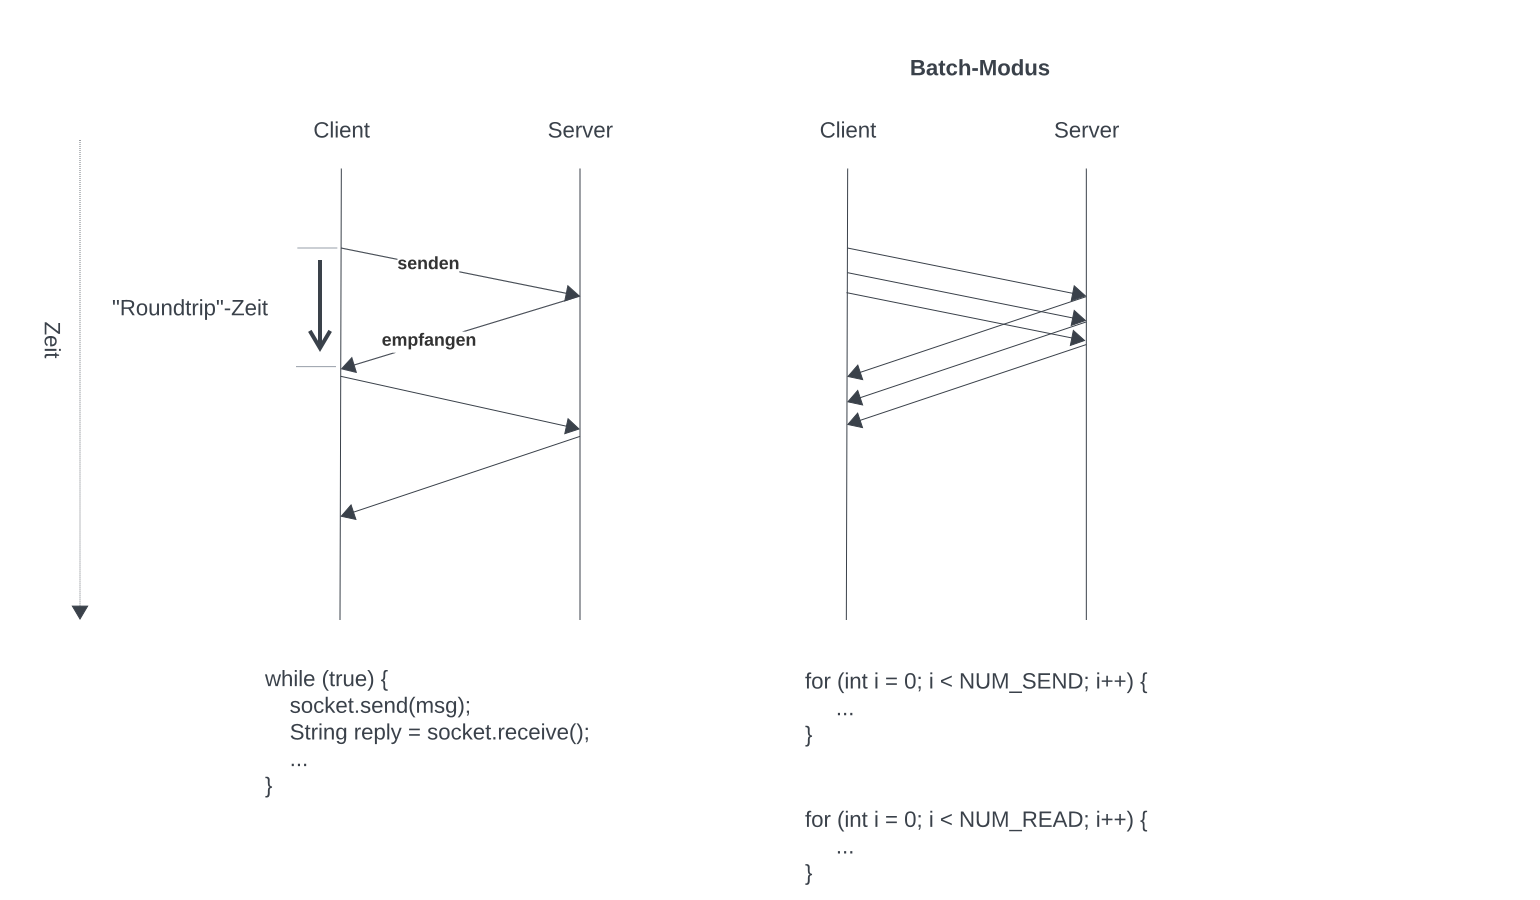
\includegraphics[scale=0.4]{chapters/Anhang/Klausuren/img/batchmodus}
    \caption{Vereinfachte Darstellung sequentieller Kommunikation und Batch-Modus (Quelle: eigene)}
    \label{fig:batchmodus}
\end{figure}
    
\begin{appendices}
    \input{chapters/Anhang/Zusatzaufgaben/index}
    \input{chapters/Anhang/Klausuren/ws13}
    \input{chapters/Anhang/Klausuren/ws15-16}
    \input{chapters/Anhang/Klausuren/ws16-17}
    \input{chapters/Anhang/Klausuren/ss19}
    \input{chapters/Anhang/Präsenzphase/index}

\end{appendices}


\end{appendices}


\end{appendices}


\begin{appendices}
    
\begin{appendices}
    
\begin{appendices}
    \input{chapters/Anhang/Zusatzaufgaben/index}
    \input{chapters/Anhang/Klausuren/ws13}
    \input{chapters/Anhang/Klausuren/ws15-16}
    \input{chapters/Anhang/Klausuren/ws16-17}
    \input{chapters/Anhang/Klausuren/ss19}
    \input{chapters/Anhang/Präsenzphase/index}

\end{appendices}

    \chapter{WS13}\label{ch:klausurws13}

\section{Aufgabe 1}
\subsection{Lösungsvorschlag}


\begin{minted}[mathescape,
    linenos,
    numbersep=5pt,
    gobble=2,
    fontsize=\small,
    frame=lines,
    framesep=2mm]{java}
    class Zahlenschloss {

        private int[] kombination;

        private int[] state;

        private boolean opened = false;

        public Zahlenschloss(int[] kombination) {
            this.kombination = kombination;
            this.state = new int[kombination.length];
        }

        public int anzahlRaedchen() {
            return kombination.length;
        }

        public synchronized int lesen(int radnummer) {
            return state[radnummer];
        }

        public synchronized void drehen(int radnummer, int zahl) {

            state[radnummer] = zahl;
            opened = true;
            for (int i = 0; i < anzahlRaedchen(); i++) {
                if (lesen(i) != kombination[i]) {
                    opened = false;
                    break;
                }
            }

            if (opened) {
                this.notify();
            }
        }

        public synchronized void warten() {

            while (!opened) {
                try {
                    this.wait();
                } catch (InterruptedException ignored) {}
            }
        }
    }
\end{minted}\\


\subsection{Anmerkung und Ergänzungen}

\begin{itemize}
    \item Es wird eine Wartebedingung benötigt, und zwar für die Methode \code{warten()}; ankommende Threads werden
    in die Warteschlange des Zahlenschloss-Objektes geschickt, wenn \code{opened} auf false gesetzt ist, ansonsten
    verlassen diese direkt die Methode wieder.\\
    Die Methode \code{drehen} benötigt keine separate Wartebedingung.
    Es reicht aus, sicherzustellen, dass das Zahlenschloss nicht gleichzeitig von anderen Threads benutzt werden kann:
    Die Methode \code{drehen} ist hierfür synchronisiert, damit das Zahlenschloss {insg.} immer nur eine Zustandsänderung
    erfährt - es sind andere Implementierungen möglich, in denen das Zahlenschloss dann von mehreren Threads gleichzeitig
    genutzt werden darf, wenn sich die Zugriffe anhand der ``Ziel``-\code{radnummer} unterscheiden, {bspw.} durch Mutex-Semaphore,
    die pro Radnummer verwendet werden\footnote{
        der gleichzeitige Zugriff auf unterschiedliche Arrays-Indizes ist erlaubt, s. `´17.4.1. Shared Variables``: \url{https://docs.oracle.com/javase/specs/jls/se21/html/jls-17.html#jls-1.4.1} - abgerufen 14.2.2024
    }.
    \item Es gibt nur eine Wartebedingung, von daher sollte \code{notify()} genügen.\\
    Wenn wir allerdings davon ausgehen, dass mehrere Threads über die Methode \code{warten()} in die Warteschlange des Objektes eingereiht worden sind,  sollte \code{notifyAll()} verwendet werden (siehe hierzu auch Abschnitt \ref{subsec:notifyAll}).
    Dennoch ist nicht garantiert, dass auch alle Threads aus der Warteschlange gelangen, denn es kann sein, dass ein anderer Thread die Methode \code{drehen()} betritt, dort die
    Zahlenkombination ändert und \code{opened} wieder auf \code{false} gesetzt wird. \\
    Ein anderer Thread, der nun in  \code{warten()} an die Reihe kommt, überprüft die Wartebedingung, und wird wieder in die Warteschlange eingereiht.
    Es ist also durchaus möglich, dass ein Thread nicht mehr aus der Methode \code{warten()} herauskommt.\\
    Dies könnte bspw. dadurch verhindert werden, dass die Threads in eine Queue gepackt werden, und in \code{drehen()} eine Wartebedingung eingefügt wird, die erst erfüllt ist,
    wenn die Queue geleert wurde oder aus ihr entnommen wurde, in der Reihenfolge, in der die Threads in die Queue eingereiht worden sind (\textit{FIFO}) (s. a. Abschnitt~\ref{subsec:readerwriterproblem}).
    \item Bei der Teilaufgabe mit der Schleife muss die komplette Schleife synchronisiert werden, was man durch ein \code{synchronized}-Statement erreicht\footnote{siehe Abschnitt~\ref{subsec:synchronizedstatement}.}
    \begin{minted}[mathescape,
        linenos,
        numbersep=5pt,
        gobble=2,
        fontsize=\small,
        frame=lines,
        framesep=2mm]{java}
        synchronized (zk) {
            for (int i = 0; i < anzahlRaedchen; i++) {
                System.out.println(zk.lesen(i));
            }
        }
    \end{minted}
    Ansonsten läuft man Gefahr, dass sich nach Auslesen der 1. Position der Wert von Position 2 geändert hat und dadurch eine
    Zahlenkombination ausgegeben wird, die es nicht gegeben hat:
    \begin{enumerate}
        \item $K\coloneqq[0, 0, 0]$
        \item Position $K_0$ wird ausgelesen und liefert $0$.
        \item Thread ändert $K_0$ zu $1$ $\implies K\coloneqq[1, 0, 0] $.
        \item Thread ändert $K_1$ zu $2$ $\implies K\coloneqq[1, 2, 0] $.
        \item Thread ändert $K_2$ zu $3$ $\implies K\coloneqq[1, 2, 3] $.
        \item Positionen $K_1$ und $K_2$ werden ausgelesen und liefern: $2, 3$
        \item Ausgabe: $0, 2, 3$ - diese Kombination hat es in dem Fall aber tatsächlich nicht gegeben.
    \end{enumerate}
\end{itemize}

\begin{tcolorbox}[colback=red!20,color=white,title=Anmerkung]
    Die Methode \code{lesen()} als \code{synchronized} zu markieren könnte man sich vlt. sparen, wenn man davon ausgeht,
    dass die Methode ohnehin in einem \code{synchronized}-Statement verwendet wird, um alle Rädchen abzulesen.\\
    Mehrere Threads können also nicht parallel auf unterschiedliche Positionen des Feldes zugreifen, wenn die Methode
    synchronisiert ist.\\
    Allerdings ist sowohl das Skript als auch das Buch recht klar, was in dieser Situation geschehen muss (s. Skript Fopt1/2, S. 9, außerdem \cite[31, Abschnitt 2.3.6]{Oec22}): Es muss (in diesem Kurs) immer \code{synchronized} verwendet werden, wenn gleichzeitig
    Daten geschrieben und gleichzeitig diese Daten gelesen werden sollen - und eine andere Implementierung, bei der die
    einzelnen Positionen ``gelocked`` sind, so dass ein gleichzeitiger Zugriff auf unterschiedliche Rädchen möglich ist, war nicht gefordert.\\
    Ggfl. würde in anderen Implementierungen der Einsatz von \code{AtomicReferenceArray}\footnote{s. \cite[157 ff.]{Oec22}
    s. ``Class AtomicReferenceArray<E>``: \url{https://docs.oracle.com/en/java/javase/21/docs/api/java.base/java/util/concurrent/atomic/AtomicReferenceArray.html} - abgerufen 15.2.2024
    } Sinn machen, aber das Lehrmaterial ist bereits sehr eindeutig bzgl. der Verwendung von \code{synchronized}.
\end{tcolorbox}



\section{Aufgabe 3}
\subsection{Lösungsvorschlag}

\subsection*{Statische Parallelität}
Statische Parallelität erlaubt es einem Server, eine \textit{fixe} Anzahl von Verbindungen gleichzeitig zu bedienen.\\
Hierbei wird ein Feld von Threads erstellt, wobei jeder Thread das \code{ServerSocket}-Objekt als Referenz übergeben bekommt.
In der \code{run()}-Methode wird dann über \code{accept()} in einer Endlosschleife auf eingehende Verbindungen gewartet, die dann so lange bedient werden, bis sich ein Client wieder abmeldet (oder eine andere Abbruchbedingung erfüllt ist, wie z.B. ein \code{SocketTimeout}).\\
Das sich ein Client abmeldet, bekommt man bspw. dadurch mit, dass \code{null} beim Lesen von einer Nachricht des Clients zurückgegeben wird (vgl. \cite[286]{Oec22}. \\
Siehe Abschnitt~\ref{sec:seqparserver} für ein Implementierungsbeispiel.



\subsection*{Dynamische Parallelität}

Bei der \textbf{Dynamischer Parallelität} erzeugt der Server für jede Verbindung einen neuen Thread, der so lange läuft, bis der Client die Verbindung wieder trennt.\\
Die Anzahl der Threads ändert sich dadurch laufend.\\
Wird die max. Anzahl erlaubter Threads nicht kontrolliert, kann es zu einer Überlastung des Server-Rechners kommen (bspw. durch einen Denial-of-Service-Angriff.)\\

\noindent
I.d.R. ist eine Mischform aus beidem geeignet, um mehrere Clients gleichzeitig bedienen zu können, und dabei nicht Gefahr zu laufen, durch dynamisches, unbegrenztes Wachstum der Anzahl der Threads überlastet zu werden.

    \chapter{WS13}\label{ch:klausurws5-16}

\section{Rechteck-Scroll (SS15 Aufgabe 2)}

Aufgabenstellung unklar.\\
Mögliche Implementierung unter \url{https://github.com/ThorstenSuckow/fopt/tree/main/src/main/java/klausurvorbereitung/foptws1516/MouseDragsSquareDemo}.

\section{Rechteck-Scroll (WS15/16 Aufgabe 1)}

Aufgabenstellung unklar.\\
Mögliche Implementierung unter \url{https://github.com/ThorstenSuckow/fopt/tree/main/src/main/java/klausurvorbereitung/foptws1516/MaxWeightDemo}.\\

\noindent
Es gibt nur eine Warteschlange für Threads in \code{use()}, es gibt keine Wartebedingung in \code{dontUse()} und damit auch keine weitere Warteschlange.\\
Es sind durch die Zugriffe auf unterschiedliche Indizes allerdings mehrere Wartebedingungen vorhanden, weshalb hab \code{notifyAll()} nutzen sollte,
sobald ein Zugriff auf ein Feld nach Aufruf von \code{dontUse} wieder möglich wird.\\
Ansonsten bestünde die Gefahr, dass bei dem Einsatz von \code{notify()} ein wartender Thread nicht geweckt wird, obwohl er weiterlaufen könnte:\\
Angenommen, das Feld $F$ hat eine Länge von $3$, das \code{maxWeight} ist mit $2$ konfiguriert.
Thread $t_1$ mit einer Laufzeit von $200\ sek$ bekommt Zugriff auf $F_0$, setzt $currentWeight$ auf $1$.\\
Thread $t_2$ mit einer Laufzeit von $1\ sek$ möchte auf $F_1$ zugreifen, setzt $currentWeight=2$ in die Warteschlange.\\
Thread $t_3$ meldet Zugriff auf $F_0$ an und gelangt in die Warteschlange.\\
Thread $t_4$ meldet Zugriff auf $F_1$ an und gelangt in die Warteschlange.\\
Thread $t_2$ ist mit der Bearbeitung von $F_1$ fertig, $currentWeight$ wird auf $1$ gesetzt, \code{notify()} wird aufgerufen.\\
Thread $t_3$ wird aus der Warteschlange geholt, kann aber nicht weiterarbeiten, da $F_0$ noch durch den länger dauernden $t_1$ blockiert ist, und kommt wieder in die Warteschlange.\\

\noindent
Offensichtlich hätte in dem Beispiel \code{notifyAll()} dazu geführt, dass auch $T_4$ seine Wartebedingung hätte überprüfen können, und hätte so Zugriff auf $F_1$ bekommen.
Stattdessen muss nun gewartet werden, bis das nächste \code{notify()} aufgerufen wird, oder ein neu ankommender Thread $F_1$ belegt.

    \chapter{WS16-17}\label{ch:klausurws16-17}

\section{Aufgabe 1}
\subsection{Lösungshinweis}

Die erste Aufgabe verdeutlicht, was bei einem \code{notifyAll()} und unsauber gesetzten Wartebedingungen passieren kann.\\
Sei folgender Quellcode gegeben:


\begin{minted}[mathescape,
    linenos,
    numbersep=5pt,
    gobble=2,
    fontsize=\small,
    frame=lines,
    framesep=2mm]{java}
    class Cond1AndCond2 {

        private boolean cond1;
        private boolean cond2;

        public synchronized void setCond1(boolean c) {
            cond1 = c;
            notifyAll();
        }

        public synchronized void setCond2(boolean c) {
            cond2 = c;
            notifyAll();
        }

        public synchronized void cond1AndCond2() {
            while(!cond1) {
                try {
                    wait();
                } catch(InterruptedException e) { }
            }

            while(!cond2) {
                try {
                    wait();
                } catch(InterruptedException e) {}
            }
            System.out.println("cond1 and cond2:" + cond1 + " " + cond2);
        }
    }
\end{minted}\\

Man sollte auf den ersten Blick meinen, dass \code{cond1} und \code{cond2} beide \code{true} sein müssen, damit die Ausgabe erfolgt.\\
Tatsächlich ist es aber so, dass es in der Methode zwei unterschiedliche Wartebedingungen gibt.\\
Die erste Wartebedingung schickt einen Thread in die Warteschlange, wenn \code{cond1 == false} gilt.\\
Setzt ein anderer Thread über \code{setCond1(true)} das Attribut entsprechend auf \code{true}, bewirkt der nachfolgende Aufruf von \code{notifyAll()}, dass alle \textit{wartenden} Threads aus der Warteschlange entfernt werden und erneut um eine Sperre des Objektes konkurrieren.\\
Erhält ein entsprechender Thread $t_w$ die Sperre auf das Objekt und kann seine \textit{while-wait-Schleife} verlassen, kann es vorkommen, dass er erneut in die Warteschlange eingereiht wird, wegen der nachfolgenden Wartebedingung \code{cond2 == false}.\\
Angenommen, ein weiterer Thread ruft nun \code{setCond2(true)} auf, und $t_w$ kommt aus der Warteschlange und konkurriert erneut und um die Sperre des Objektes, dann kann es vorkommen, das ein anderer Thread zunächst die Sperre erhält, \code{cond1} wieder auf \code{false} setzt, dann erhält $t_w$ die Sperre, überprüft die Wartebedingung \code{cond2 == false}.\\
Wegen \code{cond2} gelangt er aus der \textit{while-wait-Schleife} und die Ausgabe erfolgt - da zwischenzeitlich \code{cond1} wieder auf \code{false} gesetzt wurde, ist die erwartete Ausgabe nicht \code{true true}, sondern \code{false true} (s. Abbildung \ref{fig:cond1cond2}).\\

\begin{figure}
    \centering
    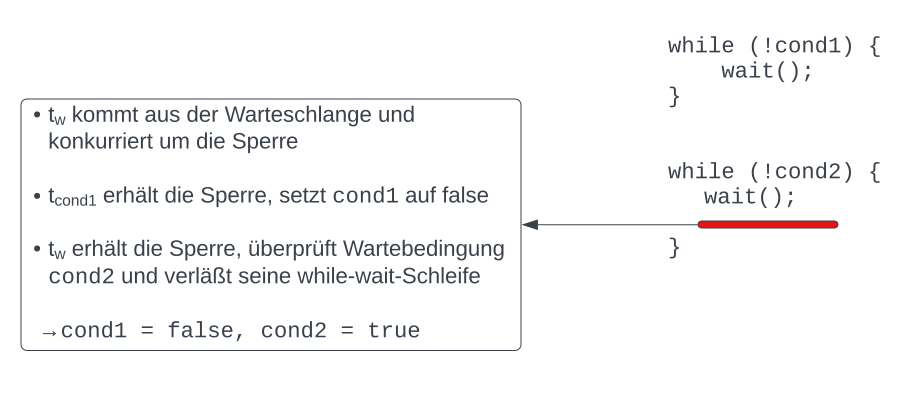
\includegraphics[scale=0.4]{chapters/Anhang/Klausuren/img/cond1cond2}
    \caption{in den rot markierten Bereich konkurriert $t_w$ um die Sperre des Objektes - wenn durch einen anderen Thread, der vor $t_w$ die Sperre erhält, \textit{cond1} auf \textit{false} gesetzt wird, stimmt die Ausgabe nicht mit der erwarteten überein. (Quelle: eigene)}
    \label{fig:cond1cond2}
\end{figure}

\noindent
Die korrekte Wartebedingung sollte lauten:

\begin{minted}[mathescape,
    linenos,
    numbersep=5pt,
    gobble=2,
    fontsize=\small,
    frame=lines,
    framesep=2mm]{java}
    public synchronized void cond1AndCond2() {
        while(!cond1 || !cond2) {
            try {
                wait();
            } catch(InterruptedException e) { }
        }
        System.out.println("cond1 and cond2:" + cond1 + " " + cond2);
    }
\end{minted}\\

Darüber hinaus müßte \code{notifyAll()} nur aufgerufen werden, wenn sowohl \code{cond1} als auch \code{cond2} auf \code{true} gesetzt sind, was leicht in den entsprechenden Methoden überprüft werden kann.
    \chapter{SS19}\label{ch:klausurss19}

\section{Aufgabe 1}

Bei der Aufgabe ist es wichtig, die Anforderungen genau zu beachten.\\
Ob eine Thread die while-wait-Schleife verlassen darf, wird von der Methode \code{tick()} gesteuert - wieviele Ticks ein Thread in der Schleife bleiben soll, wird von dem jeweiligen Thread definiert.\\
Die \code{tick()}-Methode wird von anderen Threads aufgerufen, es kann also durchaus vorkommen, dass mehrmals hintereinander
die \code{notifyAll()}-Methode aufgerufen wird - diese entfernt alle Threads aus der Warteschlange, damit die Threads ihre
Wartebedingungen erneut überprüfen können.\\
da \code{tick()} aber auch gleichzeitig einen Zähler realisieren soll, \textit{muss} es in der Methode auch eine Zählvariable geben, anhand derer die in der while-wait-Schleife enthaltenen Threads feststellen können, wie oft \code{tick()} aufgerufen wurde, um entsprechend aus der Schleife und nachfolgend der Methode herauszukommen.

\begin{figure}
    \centering
    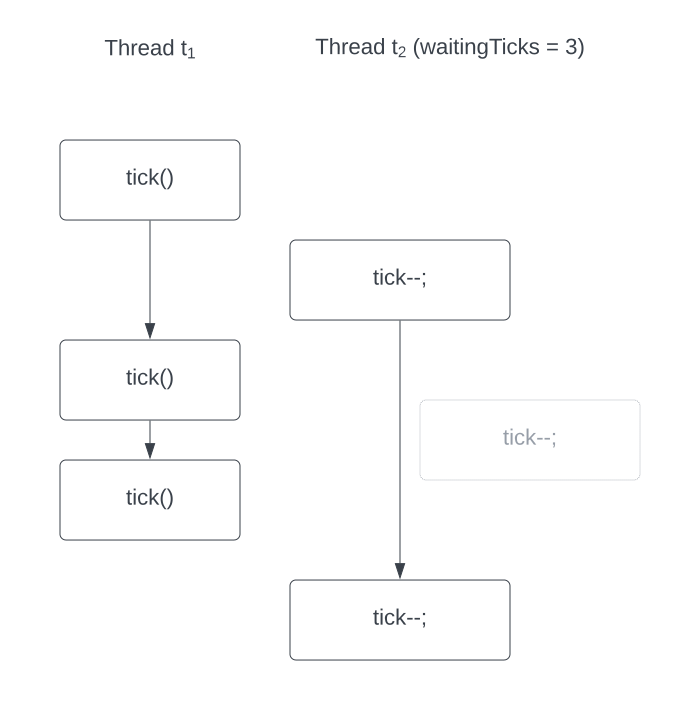
\includegraphics[scale=0.5]{chapters/Anhang/Klausuren/img/tick}
    \caption{Thread $t_1$ ruft 3 mal \texit{tick()} auf. Den Anforderungen nach müsste Thread $t_2$ danach aus der while-wait-Schleife herauskommen, erhält aber nicht die Sperre auf das Objekt von LogicalTime, um seinen eigenen Zähler rechtzeitig zu erniedrigen, bevor $t_1$ erneut \textit{tick()} aufruft. (Quelle: eigene)}
    \label{fig:tick}
\end{figure}

\section{Aufgabe 6}
Auch hier gilt, dass die Aufgabenstellung aufmerksam zu lesen ist.\\
Der Kreis soll erst ausgefüllt werden, wenn die Maustaste gelöst wird.

\begin{minted}[mathescape,
    linenos,
    numbersep=5pt,
    gobble=2,
    frame=lines,
    framesep=2mm]{java}
    private void mousePressed(double x, double y) {
        c = new Circle();
        c.setCenterX(x);
        c.setCenterY(y);
        c.setStroke(Color.RED);
        c.setFill(null); // oder Color.TRANSPARENT
        c.setRadius(RADIUS);
        graphicsPane.getChildren().add(c);
    }

    private void mouseReleased() {
        c.setFill(Color.RED);
        c = null;
    }
\end{minted}

\section{Aufgabe 8}

In der Abbildung \ref{fig:batchmodus} ist links der sequentielle Modus dargestellt, bei dem nach dem Senden einer Nachricht auf die Antwort des Servers gewartet wird, bevor eine neue Nachricht geschickt wird.
Dies wird i.d.R. verwendet, wenn das Senden einer neuen Nachricht abhängig ist von einem Ergebnis, die über die Server-Antwort übermittelt wird, oder wenn mit dem Server interagiert wird (Request abhängig vom Response).\\
Der Batch-Modus auf der rechten Seite der gleichen Abbildung ist schneller, da zwischen dem Senden von Nachrichten nicht auf Antworten gewartet werden müssen. \\
Erst nach dem Senden eine Batches von Nachrichten werden die dem Client zur Verfügung stehenden Antworten ausgelesen.\\

\noindent
In dieser Form des Batch-Modus besteht allerdings die Gefahr, dass es zu Verklemmungen kommt:
\begin{itemize}
    \item Bei dem Client kommen viele Nachrichten an, während er noch sendet.
    \item Die ankommenden Nachrichten für den Client werden gepuffert, bis sie ausgelesen werden (TCP- / OS-seitig).
    \item Läuft der Puffer voll, sorgt die Flusskontrolle (TCP) dafür, dass dem Sender mitgeteilt wird, dass keine Nachrichten mehr empfangen werden können, der Server sendet nicht mehr.
    \item Die zu sendenden Nachrichten des Servers werden in einen Puffer geschrieben.
    \item Der Sende-Puffer des Senders läuft voll.
    \item Bei dem nächsten Sende-Aufruf blockiert der Server, empfangene Nachrichten landen im Empfangspuffer
    \item Der Empfangspuffer des Servers läuft voll, der Client buffert die zu sendenden Nachrichten.
    \item Beide Anwendungen blockieren.
\end{itemize}

\\noindent
Um dieses Problem beim Batch-Modus zu umgehen, werden für das Senden und Empfangen zwei Threads auf Client-Seite erstellt: Ein Thread sendet, ein Thread empfängt. \\
Dadurch kann von dem Client immer wieder sein Empfangspuffer geleert werden, der Server wird beim Senden nicht blockiert.

\begin{figure}
    \centering
    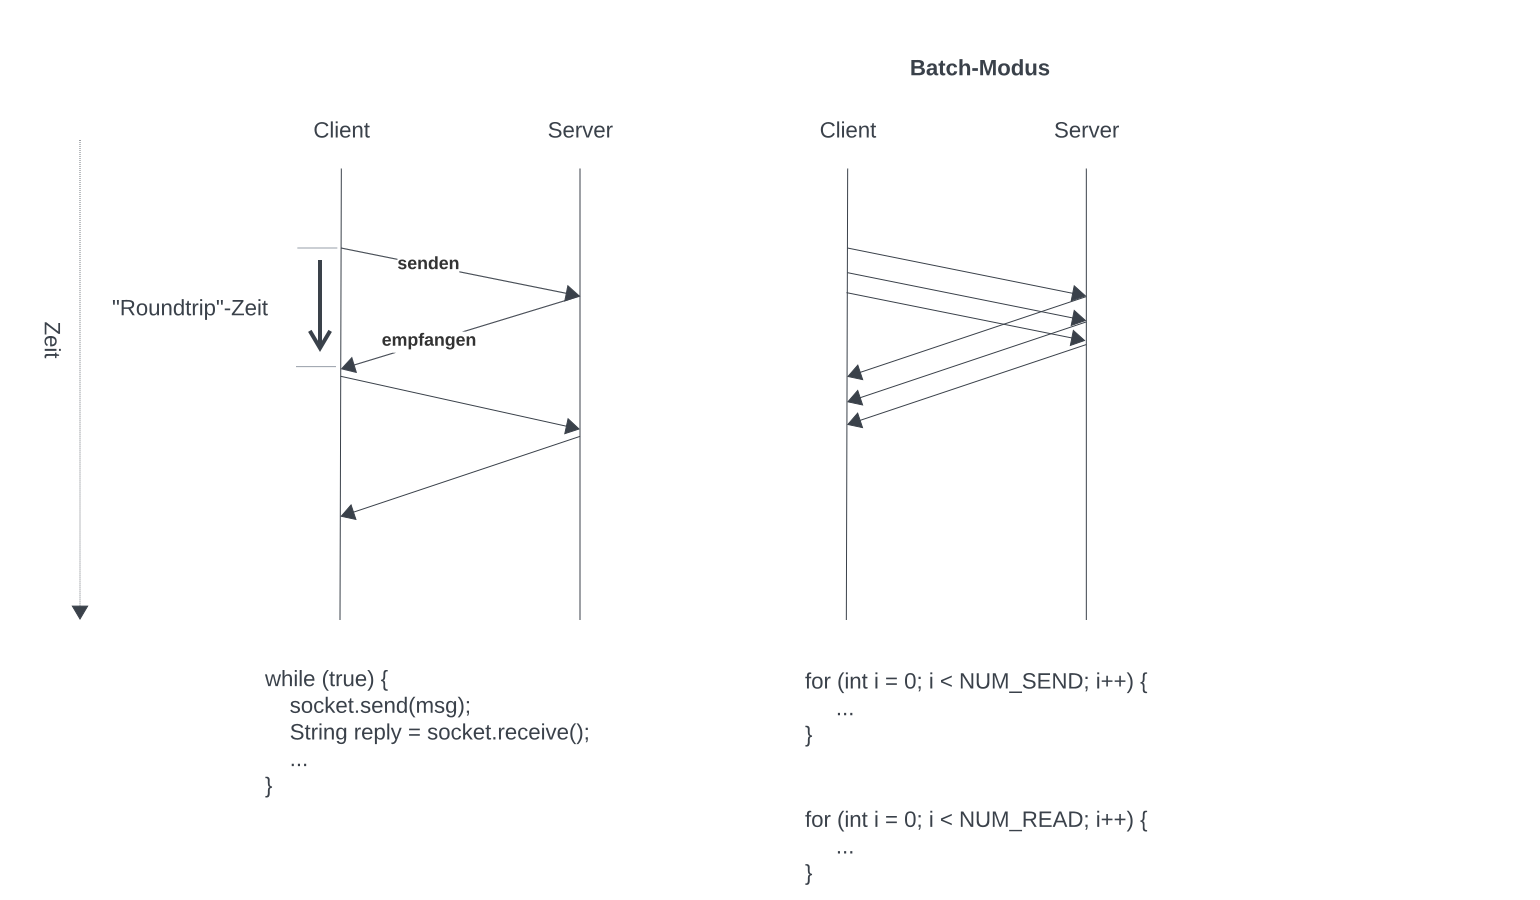
\includegraphics[scale=0.4]{chapters/Anhang/Klausuren/img/batchmodus}
    \caption{Vereinfachte Darstellung sequentieller Kommunikation und Batch-Modus (Quelle: eigene)}
    \label{fig:batchmodus}
\end{figure}
    
\begin{appendices}
    \input{chapters/Anhang/Zusatzaufgaben/index}
    \input{chapters/Anhang/Klausuren/ws13}
    \input{chapters/Anhang/Klausuren/ws15-16}
    \input{chapters/Anhang/Klausuren/ws16-17}
    \input{chapters/Anhang/Klausuren/ss19}
    \input{chapters/Anhang/Präsenzphase/index}

\end{appendices}


\end{appendices}

    \chapter{WS13}\label{ch:klausurws13}

\section{Aufgabe 1}
\subsection{Lösungsvorschlag}


\begin{minted}[mathescape,
    linenos,
    numbersep=5pt,
    gobble=2,
    fontsize=\small,
    frame=lines,
    framesep=2mm]{java}
    class Zahlenschloss {

        private int[] kombination;

        private int[] state;

        private boolean opened = false;

        public Zahlenschloss(int[] kombination) {
            this.kombination = kombination;
            this.state = new int[kombination.length];
        }

        public int anzahlRaedchen() {
            return kombination.length;
        }

        public synchronized int lesen(int radnummer) {
            return state[radnummer];
        }

        public synchronized void drehen(int radnummer, int zahl) {

            state[radnummer] = zahl;
            opened = true;
            for (int i = 0; i < anzahlRaedchen(); i++) {
                if (lesen(i) != kombination[i]) {
                    opened = false;
                    break;
                }
            }

            if (opened) {
                this.notify();
            }
        }

        public synchronized void warten() {

            while (!opened) {
                try {
                    this.wait();
                } catch (InterruptedException ignored) {}
            }
        }
    }
\end{minted}\\


\subsection{Anmerkung und Ergänzungen}

\begin{itemize}
    \item Es wird eine Wartebedingung benötigt, und zwar für die Methode \code{warten()}; ankommende Threads werden
    in die Warteschlange des Zahlenschloss-Objektes geschickt, wenn \code{opened} auf false gesetzt ist, ansonsten
    verlassen diese direkt die Methode wieder.\\
    Die Methode \code{drehen} benötigt keine separate Wartebedingung.
    Es reicht aus, sicherzustellen, dass das Zahlenschloss nicht gleichzeitig von anderen Threads benutzt werden kann:
    Die Methode \code{drehen} ist hierfür synchronisiert, damit das Zahlenschloss {insg.} immer nur eine Zustandsänderung
    erfährt - es sind andere Implementierungen möglich, in denen das Zahlenschloss dann von mehreren Threads gleichzeitig
    genutzt werden darf, wenn sich die Zugriffe anhand der ``Ziel``-\code{radnummer} unterscheiden, {bspw.} durch Mutex-Semaphore,
    die pro Radnummer verwendet werden\footnote{
        der gleichzeitige Zugriff auf unterschiedliche Arrays-Indizes ist erlaubt, s. `´17.4.1. Shared Variables``: \url{https://docs.oracle.com/javase/specs/jls/se21/html/jls-17.html#jls-1.4.1} - abgerufen 14.2.2024
    }.
    \item Es gibt nur eine Wartebedingung, von daher sollte \code{notify()} genügen.\\
    Wenn wir allerdings davon ausgehen, dass mehrere Threads über die Methode \code{warten()} in die Warteschlange des Objektes eingereiht worden sind,  sollte \code{notifyAll()} verwendet werden (siehe hierzu auch Abschnitt \ref{subsec:notifyAll}).
    Dennoch ist nicht garantiert, dass auch alle Threads aus der Warteschlange gelangen, denn es kann sein, dass ein anderer Thread die Methode \code{drehen()} betritt, dort die
    Zahlenkombination ändert und \code{opened} wieder auf \code{false} gesetzt wird. \\
    Ein anderer Thread, der nun in  \code{warten()} an die Reihe kommt, überprüft die Wartebedingung, und wird wieder in die Warteschlange eingereiht.
    Es ist also durchaus möglich, dass ein Thread nicht mehr aus der Methode \code{warten()} herauskommt.\\
    Dies könnte bspw. dadurch verhindert werden, dass die Threads in eine Queue gepackt werden, und in \code{drehen()} eine Wartebedingung eingefügt wird, die erst erfüllt ist,
    wenn die Queue geleert wurde oder aus ihr entnommen wurde, in der Reihenfolge, in der die Threads in die Queue eingereiht worden sind (\textit{FIFO}) (s. a. Abschnitt~\ref{subsec:readerwriterproblem}).
    \item Bei der Teilaufgabe mit der Schleife muss die komplette Schleife synchronisiert werden, was man durch ein \code{synchronized}-Statement erreicht\footnote{siehe Abschnitt~\ref{subsec:synchronizedstatement}.}
    \begin{minted}[mathescape,
        linenos,
        numbersep=5pt,
        gobble=2,
        fontsize=\small,
        frame=lines,
        framesep=2mm]{java}
        synchronized (zk) {
            for (int i = 0; i < anzahlRaedchen; i++) {
                System.out.println(zk.lesen(i));
            }
        }
    \end{minted}
    Ansonsten läuft man Gefahr, dass sich nach Auslesen der 1. Position der Wert von Position 2 geändert hat und dadurch eine
    Zahlenkombination ausgegeben wird, die es nicht gegeben hat:
    \begin{enumerate}
        \item $K\coloneqq[0, 0, 0]$
        \item Position $K_0$ wird ausgelesen und liefert $0$.
        \item Thread ändert $K_0$ zu $1$ $\implies K\coloneqq[1, 0, 0] $.
        \item Thread ändert $K_1$ zu $2$ $\implies K\coloneqq[1, 2, 0] $.
        \item Thread ändert $K_2$ zu $3$ $\implies K\coloneqq[1, 2, 3] $.
        \item Positionen $K_1$ und $K_2$ werden ausgelesen und liefern: $2, 3$
        \item Ausgabe: $0, 2, 3$ - diese Kombination hat es in dem Fall aber tatsächlich nicht gegeben.
    \end{enumerate}
\end{itemize}

\begin{tcolorbox}[colback=red!20,color=white,title=Anmerkung]
    Die Methode \code{lesen()} als \code{synchronized} zu markieren könnte man sich vlt. sparen, wenn man davon ausgeht,
    dass die Methode ohnehin in einem \code{synchronized}-Statement verwendet wird, um alle Rädchen abzulesen.\\
    Mehrere Threads können also nicht parallel auf unterschiedliche Positionen des Feldes zugreifen, wenn die Methode
    synchronisiert ist.\\
    Allerdings ist sowohl das Skript als auch das Buch recht klar, was in dieser Situation geschehen muss (s. Skript Fopt1/2, S. 9, außerdem \cite[31, Abschnitt 2.3.6]{Oec22}): Es muss (in diesem Kurs) immer \code{synchronized} verwendet werden, wenn gleichzeitig
    Daten geschrieben und gleichzeitig diese Daten gelesen werden sollen - und eine andere Implementierung, bei der die
    einzelnen Positionen ``gelocked`` sind, so dass ein gleichzeitiger Zugriff auf unterschiedliche Rädchen möglich ist, war nicht gefordert.\\
    Ggfl. würde in anderen Implementierungen der Einsatz von \code{AtomicReferenceArray}\footnote{s. \cite[157 ff.]{Oec22}
    s. ``Class AtomicReferenceArray<E>``: \url{https://docs.oracle.com/en/java/javase/21/docs/api/java.base/java/util/concurrent/atomic/AtomicReferenceArray.html} - abgerufen 15.2.2024
    } Sinn machen, aber das Lehrmaterial ist bereits sehr eindeutig bzgl. der Verwendung von \code{synchronized}.
\end{tcolorbox}



\section{Aufgabe 3}
\subsection{Lösungsvorschlag}

\subsection*{Statische Parallelität}
Statische Parallelität erlaubt es einem Server, eine \textit{fixe} Anzahl von Verbindungen gleichzeitig zu bedienen.\\
Hierbei wird ein Feld von Threads erstellt, wobei jeder Thread das \code{ServerSocket}-Objekt als Referenz übergeben bekommt.
In der \code{run()}-Methode wird dann über \code{accept()} in einer Endlosschleife auf eingehende Verbindungen gewartet, die dann so lange bedient werden, bis sich ein Client wieder abmeldet (oder eine andere Abbruchbedingung erfüllt ist, wie z.B. ein \code{SocketTimeout}).\\
Das sich ein Client abmeldet, bekommt man bspw. dadurch mit, dass \code{null} beim Lesen von einer Nachricht des Clients zurückgegeben wird (vgl. \cite[286]{Oec22}. \\
Siehe Abschnitt~\ref{sec:seqparserver} für ein Implementierungsbeispiel.



\subsection*{Dynamische Parallelität}

Bei der \textbf{Dynamischer Parallelität} erzeugt der Server für jede Verbindung einen neuen Thread, der so lange läuft, bis der Client die Verbindung wieder trennt.\\
Die Anzahl der Threads ändert sich dadurch laufend.\\
Wird die max. Anzahl erlaubter Threads nicht kontrolliert, kann es zu einer Überlastung des Server-Rechners kommen (bspw. durch einen Denial-of-Service-Angriff.)\\

\noindent
I.d.R. ist eine Mischform aus beidem geeignet, um mehrere Clients gleichzeitig bedienen zu können, und dabei nicht Gefahr zu laufen, durch dynamisches, unbegrenztes Wachstum der Anzahl der Threads überlastet zu werden.

    \chapter{WS13}\label{ch:klausurws5-16}

\section{Rechteck-Scroll (SS15 Aufgabe 2)}

Aufgabenstellung unklar.\\
Mögliche Implementierung unter \url{https://github.com/ThorstenSuckow/fopt/tree/main/src/main/java/klausurvorbereitung/foptws1516/MouseDragsSquareDemo}.

\section{Rechteck-Scroll (WS15/16 Aufgabe 1)}

Aufgabenstellung unklar.\\
Mögliche Implementierung unter \url{https://github.com/ThorstenSuckow/fopt/tree/main/src/main/java/klausurvorbereitung/foptws1516/MaxWeightDemo}.\\

\noindent
Es gibt nur eine Warteschlange für Threads in \code{use()}, es gibt keine Wartebedingung in \code{dontUse()} und damit auch keine weitere Warteschlange.\\
Es sind durch die Zugriffe auf unterschiedliche Indizes allerdings mehrere Wartebedingungen vorhanden, weshalb hab \code{notifyAll()} nutzen sollte,
sobald ein Zugriff auf ein Feld nach Aufruf von \code{dontUse} wieder möglich wird.\\
Ansonsten bestünde die Gefahr, dass bei dem Einsatz von \code{notify()} ein wartender Thread nicht geweckt wird, obwohl er weiterlaufen könnte:\\
Angenommen, das Feld $F$ hat eine Länge von $3$, das \code{maxWeight} ist mit $2$ konfiguriert.
Thread $t_1$ mit einer Laufzeit von $200\ sek$ bekommt Zugriff auf $F_0$, setzt $currentWeight$ auf $1$.\\
Thread $t_2$ mit einer Laufzeit von $1\ sek$ möchte auf $F_1$ zugreifen, setzt $currentWeight=2$ in die Warteschlange.\\
Thread $t_3$ meldet Zugriff auf $F_0$ an und gelangt in die Warteschlange.\\
Thread $t_4$ meldet Zugriff auf $F_1$ an und gelangt in die Warteschlange.\\
Thread $t_2$ ist mit der Bearbeitung von $F_1$ fertig, $currentWeight$ wird auf $1$ gesetzt, \code{notify()} wird aufgerufen.\\
Thread $t_3$ wird aus der Warteschlange geholt, kann aber nicht weiterarbeiten, da $F_0$ noch durch den länger dauernden $t_1$ blockiert ist, und kommt wieder in die Warteschlange.\\

\noindent
Offensichtlich hätte in dem Beispiel \code{notifyAll()} dazu geführt, dass auch $T_4$ seine Wartebedingung hätte überprüfen können, und hätte so Zugriff auf $F_1$ bekommen.
Stattdessen muss nun gewartet werden, bis das nächste \code{notify()} aufgerufen wird, oder ein neu ankommender Thread $F_1$ belegt.

    \chapter{WS16-17}\label{ch:klausurws16-17}

\section{Aufgabe 1}
\subsection{Lösungshinweis}

Die erste Aufgabe verdeutlicht, was bei einem \code{notifyAll()} und unsauber gesetzten Wartebedingungen passieren kann.\\
Sei folgender Quellcode gegeben:


\begin{minted}[mathescape,
    linenos,
    numbersep=5pt,
    gobble=2,
    fontsize=\small,
    frame=lines,
    framesep=2mm]{java}
    class Cond1AndCond2 {

        private boolean cond1;
        private boolean cond2;

        public synchronized void setCond1(boolean c) {
            cond1 = c;
            notifyAll();
        }

        public synchronized void setCond2(boolean c) {
            cond2 = c;
            notifyAll();
        }

        public synchronized void cond1AndCond2() {
            while(!cond1) {
                try {
                    wait();
                } catch(InterruptedException e) { }
            }

            while(!cond2) {
                try {
                    wait();
                } catch(InterruptedException e) {}
            }
            System.out.println("cond1 and cond2:" + cond1 + " " + cond2);
        }
    }
\end{minted}\\

Man sollte auf den ersten Blick meinen, dass \code{cond1} und \code{cond2} beide \code{true} sein müssen, damit die Ausgabe erfolgt.\\
Tatsächlich ist es aber so, dass es in der Methode zwei unterschiedliche Wartebedingungen gibt.\\
Die erste Wartebedingung schickt einen Thread in die Warteschlange, wenn \code{cond1 == false} gilt.\\
Setzt ein anderer Thread über \code{setCond1(true)} das Attribut entsprechend auf \code{true}, bewirkt der nachfolgende Aufruf von \code{notifyAll()}, dass alle \textit{wartenden} Threads aus der Warteschlange entfernt werden und erneut um eine Sperre des Objektes konkurrieren.\\
Erhält ein entsprechender Thread $t_w$ die Sperre auf das Objekt und kann seine \textit{while-wait-Schleife} verlassen, kann es vorkommen, dass er erneut in die Warteschlange eingereiht wird, wegen der nachfolgenden Wartebedingung \code{cond2 == false}.\\
Angenommen, ein weiterer Thread ruft nun \code{setCond2(true)} auf, und $t_w$ kommt aus der Warteschlange und konkurriert erneut und um die Sperre des Objektes, dann kann es vorkommen, das ein anderer Thread zunächst die Sperre erhält, \code{cond1} wieder auf \code{false} setzt, dann erhält $t_w$ die Sperre, überprüft die Wartebedingung \code{cond2 == false}.\\
Wegen \code{cond2} gelangt er aus der \textit{while-wait-Schleife} und die Ausgabe erfolgt - da zwischenzeitlich \code{cond1} wieder auf \code{false} gesetzt wurde, ist die erwartete Ausgabe nicht \code{true true}, sondern \code{false true} (s. Abbildung \ref{fig:cond1cond2}).\\

\begin{figure}
    \centering
    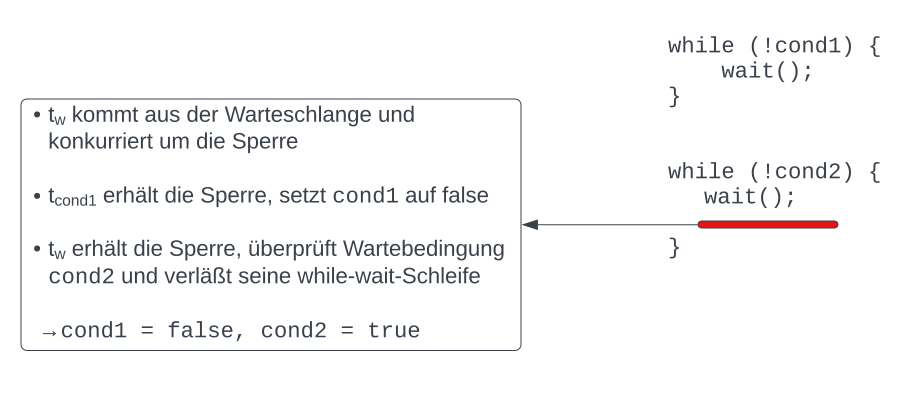
\includegraphics[scale=0.4]{chapters/Anhang/Klausuren/img/cond1cond2}
    \caption{in den rot markierten Bereich konkurriert $t_w$ um die Sperre des Objektes - wenn durch einen anderen Thread, der vor $t_w$ die Sperre erhält, \textit{cond1} auf \textit{false} gesetzt wird, stimmt die Ausgabe nicht mit der erwarteten überein. (Quelle: eigene)}
    \label{fig:cond1cond2}
\end{figure}

\noindent
Die korrekte Wartebedingung sollte lauten:

\begin{minted}[mathescape,
    linenos,
    numbersep=5pt,
    gobble=2,
    fontsize=\small,
    frame=lines,
    framesep=2mm]{java}
    public synchronized void cond1AndCond2() {
        while(!cond1 || !cond2) {
            try {
                wait();
            } catch(InterruptedException e) { }
        }
        System.out.println("cond1 and cond2:" + cond1 + " " + cond2);
    }
\end{minted}\\

Darüber hinaus müßte \code{notifyAll()} nur aufgerufen werden, wenn sowohl \code{cond1} als auch \code{cond2} auf \code{true} gesetzt sind, was leicht in den entsprechenden Methoden überprüft werden kann.
    \chapter{SS19}\label{ch:klausurss19}

\section{Aufgabe 1}

Bei der Aufgabe ist es wichtig, die Anforderungen genau zu beachten.\\
Ob eine Thread die while-wait-Schleife verlassen darf, wird von der Methode \code{tick()} gesteuert - wieviele Ticks ein Thread in der Schleife bleiben soll, wird von dem jeweiligen Thread definiert.\\
Die \code{tick()}-Methode wird von anderen Threads aufgerufen, es kann also durchaus vorkommen, dass mehrmals hintereinander
die \code{notifyAll()}-Methode aufgerufen wird - diese entfernt alle Threads aus der Warteschlange, damit die Threads ihre
Wartebedingungen erneut überprüfen können.\\
da \code{tick()} aber auch gleichzeitig einen Zähler realisieren soll, \textit{muss} es in der Methode auch eine Zählvariable geben, anhand derer die in der while-wait-Schleife enthaltenen Threads feststellen können, wie oft \code{tick()} aufgerufen wurde, um entsprechend aus der Schleife und nachfolgend der Methode herauszukommen.

\begin{figure}
    \centering
    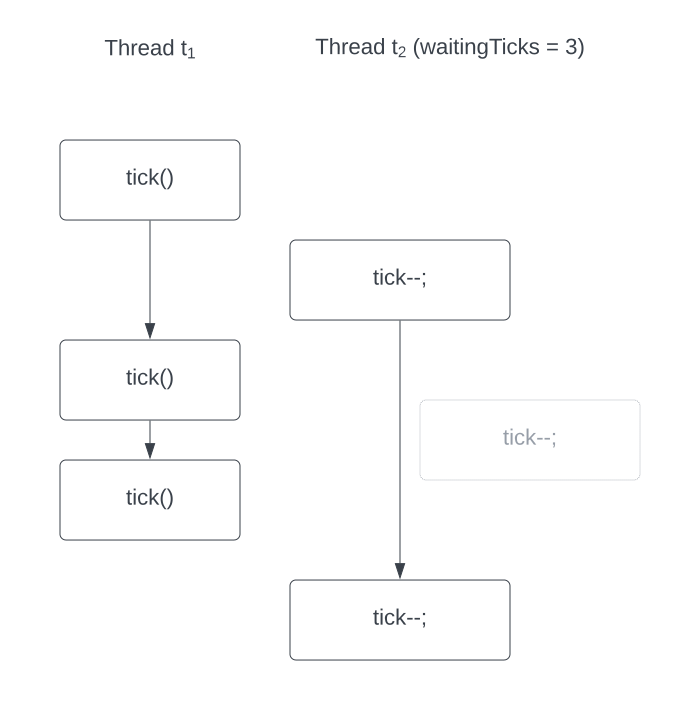
\includegraphics[scale=0.5]{chapters/Anhang/Klausuren/img/tick}
    \caption{Thread $t_1$ ruft 3 mal \texit{tick()} auf. Den Anforderungen nach müsste Thread $t_2$ danach aus der while-wait-Schleife herauskommen, erhält aber nicht die Sperre auf das Objekt von LogicalTime, um seinen eigenen Zähler rechtzeitig zu erniedrigen, bevor $t_1$ erneut \textit{tick()} aufruft. (Quelle: eigene)}
    \label{fig:tick}
\end{figure}

\section{Aufgabe 6}
Auch hier gilt, dass die Aufgabenstellung aufmerksam zu lesen ist.\\
Der Kreis soll erst ausgefüllt werden, wenn die Maustaste gelöst wird.

\begin{minted}[mathescape,
    linenos,
    numbersep=5pt,
    gobble=2,
    frame=lines,
    framesep=2mm]{java}
    private void mousePressed(double x, double y) {
        c = new Circle();
        c.setCenterX(x);
        c.setCenterY(y);
        c.setStroke(Color.RED);
        c.setFill(null); // oder Color.TRANSPARENT
        c.setRadius(RADIUS);
        graphicsPane.getChildren().add(c);
    }

    private void mouseReleased() {
        c.setFill(Color.RED);
        c = null;
    }
\end{minted}

\section{Aufgabe 8}

In der Abbildung \ref{fig:batchmodus} ist links der sequentielle Modus dargestellt, bei dem nach dem Senden einer Nachricht auf die Antwort des Servers gewartet wird, bevor eine neue Nachricht geschickt wird.
Dies wird i.d.R. verwendet, wenn das Senden einer neuen Nachricht abhängig ist von einem Ergebnis, die über die Server-Antwort übermittelt wird, oder wenn mit dem Server interagiert wird (Request abhängig vom Response).\\
Der Batch-Modus auf der rechten Seite der gleichen Abbildung ist schneller, da zwischen dem Senden von Nachrichten nicht auf Antworten gewartet werden müssen. \\
Erst nach dem Senden eine Batches von Nachrichten werden die dem Client zur Verfügung stehenden Antworten ausgelesen.\\

\noindent
In dieser Form des Batch-Modus besteht allerdings die Gefahr, dass es zu Verklemmungen kommt:
\begin{itemize}
    \item Bei dem Client kommen viele Nachrichten an, während er noch sendet.
    \item Die ankommenden Nachrichten für den Client werden gepuffert, bis sie ausgelesen werden (TCP- / OS-seitig).
    \item Läuft der Puffer voll, sorgt die Flusskontrolle (TCP) dafür, dass dem Sender mitgeteilt wird, dass keine Nachrichten mehr empfangen werden können, der Server sendet nicht mehr.
    \item Die zu sendenden Nachrichten des Servers werden in einen Puffer geschrieben.
    \item Der Sende-Puffer des Senders läuft voll.
    \item Bei dem nächsten Sende-Aufruf blockiert der Server, empfangene Nachrichten landen im Empfangspuffer
    \item Der Empfangspuffer des Servers läuft voll, der Client buffert die zu sendenden Nachrichten.
    \item Beide Anwendungen blockieren.
\end{itemize}

\\noindent
Um dieses Problem beim Batch-Modus zu umgehen, werden für das Senden und Empfangen zwei Threads auf Client-Seite erstellt: Ein Thread sendet, ein Thread empfängt. \\
Dadurch kann von dem Client immer wieder sein Empfangspuffer geleert werden, der Server wird beim Senden nicht blockiert.

\begin{figure}
    \centering
    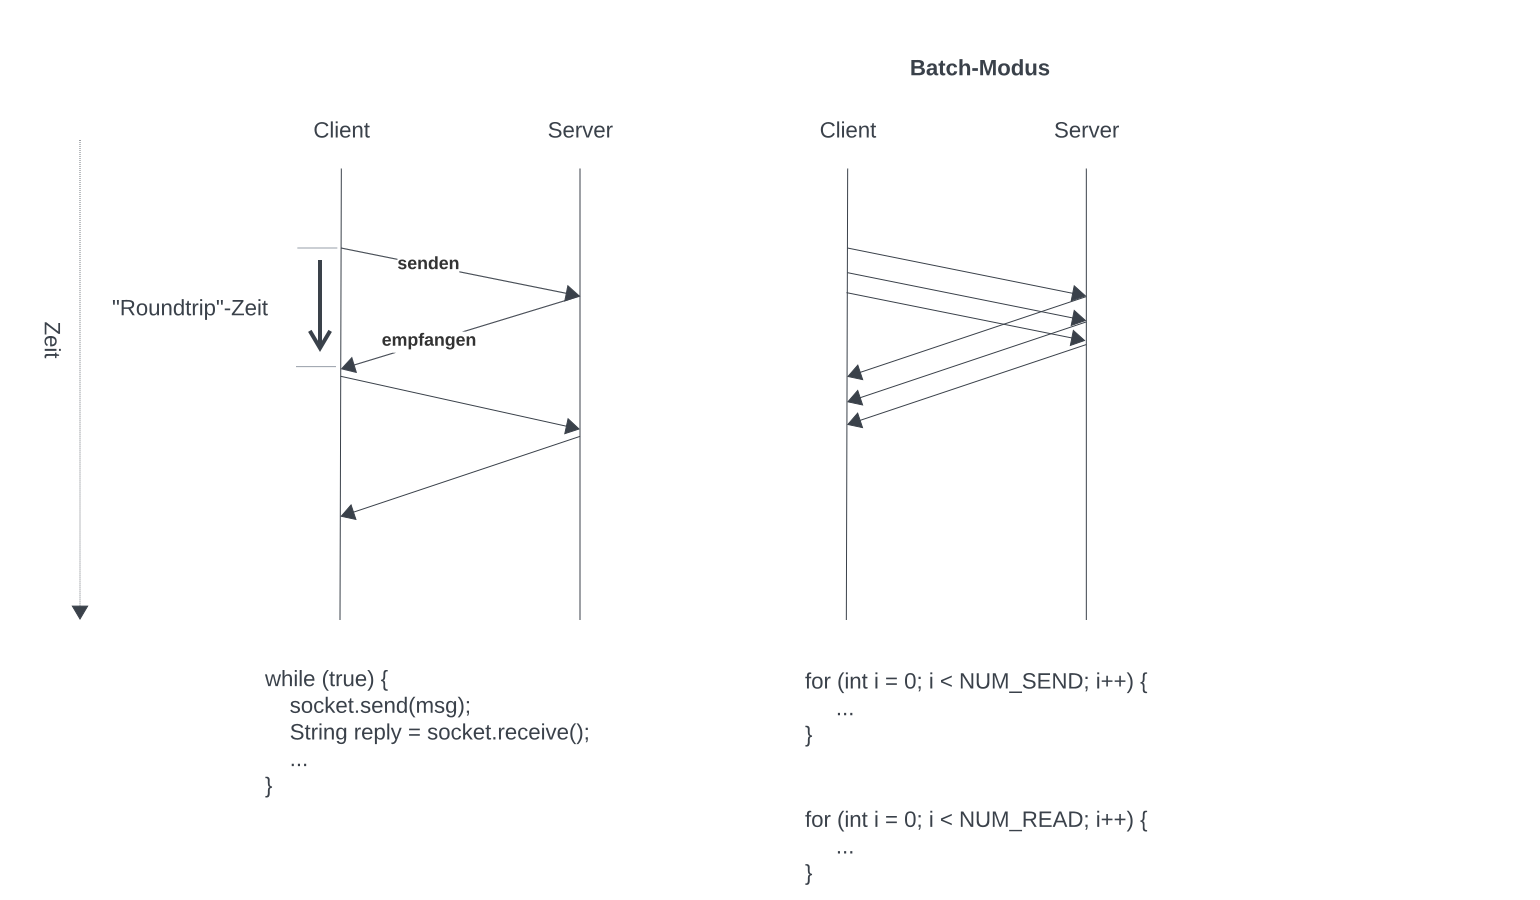
\includegraphics[scale=0.4]{chapters/Anhang/Klausuren/img/batchmodus}
    \caption{Vereinfachte Darstellung sequentieller Kommunikation und Batch-Modus (Quelle: eigene)}
    \label{fig:batchmodus}
\end{figure}
    
\begin{appendices}
    
\begin{appendices}
    \input{chapters/Anhang/Zusatzaufgaben/index}
    \input{chapters/Anhang/Klausuren/ws13}
    \input{chapters/Anhang/Klausuren/ws15-16}
    \input{chapters/Anhang/Klausuren/ws16-17}
    \input{chapters/Anhang/Klausuren/ss19}
    \input{chapters/Anhang/Präsenzphase/index}

\end{appendices}

    \chapter{WS13}\label{ch:klausurws13}

\section{Aufgabe 1}
\subsection{Lösungsvorschlag}


\begin{minted}[mathescape,
    linenos,
    numbersep=5pt,
    gobble=2,
    fontsize=\small,
    frame=lines,
    framesep=2mm]{java}
    class Zahlenschloss {

        private int[] kombination;

        private int[] state;

        private boolean opened = false;

        public Zahlenschloss(int[] kombination) {
            this.kombination = kombination;
            this.state = new int[kombination.length];
        }

        public int anzahlRaedchen() {
            return kombination.length;
        }

        public synchronized int lesen(int radnummer) {
            return state[radnummer];
        }

        public synchronized void drehen(int radnummer, int zahl) {

            state[radnummer] = zahl;
            opened = true;
            for (int i = 0; i < anzahlRaedchen(); i++) {
                if (lesen(i) != kombination[i]) {
                    opened = false;
                    break;
                }
            }

            if (opened) {
                this.notify();
            }
        }

        public synchronized void warten() {

            while (!opened) {
                try {
                    this.wait();
                } catch (InterruptedException ignored) {}
            }
        }
    }
\end{minted}\\


\subsection{Anmerkung und Ergänzungen}

\begin{itemize}
    \item Es wird eine Wartebedingung benötigt, und zwar für die Methode \code{warten()}; ankommende Threads werden
    in die Warteschlange des Zahlenschloss-Objektes geschickt, wenn \code{opened} auf false gesetzt ist, ansonsten
    verlassen diese direkt die Methode wieder.\\
    Die Methode \code{drehen} benötigt keine separate Wartebedingung.
    Es reicht aus, sicherzustellen, dass das Zahlenschloss nicht gleichzeitig von anderen Threads benutzt werden kann:
    Die Methode \code{drehen} ist hierfür synchronisiert, damit das Zahlenschloss {insg.} immer nur eine Zustandsänderung
    erfährt - es sind andere Implementierungen möglich, in denen das Zahlenschloss dann von mehreren Threads gleichzeitig
    genutzt werden darf, wenn sich die Zugriffe anhand der ``Ziel``-\code{radnummer} unterscheiden, {bspw.} durch Mutex-Semaphore,
    die pro Radnummer verwendet werden\footnote{
        der gleichzeitige Zugriff auf unterschiedliche Arrays-Indizes ist erlaubt, s. `´17.4.1. Shared Variables``: \url{https://docs.oracle.com/javase/specs/jls/se21/html/jls-17.html#jls-1.4.1} - abgerufen 14.2.2024
    }.
    \item Es gibt nur eine Wartebedingung, von daher sollte \code{notify()} genügen.\\
    Wenn wir allerdings davon ausgehen, dass mehrere Threads über die Methode \code{warten()} in die Warteschlange des Objektes eingereiht worden sind,  sollte \code{notifyAll()} verwendet werden (siehe hierzu auch Abschnitt \ref{subsec:notifyAll}).
    Dennoch ist nicht garantiert, dass auch alle Threads aus der Warteschlange gelangen, denn es kann sein, dass ein anderer Thread die Methode \code{drehen()} betritt, dort die
    Zahlenkombination ändert und \code{opened} wieder auf \code{false} gesetzt wird. \\
    Ein anderer Thread, der nun in  \code{warten()} an die Reihe kommt, überprüft die Wartebedingung, und wird wieder in die Warteschlange eingereiht.
    Es ist also durchaus möglich, dass ein Thread nicht mehr aus der Methode \code{warten()} herauskommt.\\
    Dies könnte bspw. dadurch verhindert werden, dass die Threads in eine Queue gepackt werden, und in \code{drehen()} eine Wartebedingung eingefügt wird, die erst erfüllt ist,
    wenn die Queue geleert wurde oder aus ihr entnommen wurde, in der Reihenfolge, in der die Threads in die Queue eingereiht worden sind (\textit{FIFO}) (s. a. Abschnitt~\ref{subsec:readerwriterproblem}).
    \item Bei der Teilaufgabe mit der Schleife muss die komplette Schleife synchronisiert werden, was man durch ein \code{synchronized}-Statement erreicht\footnote{siehe Abschnitt~\ref{subsec:synchronizedstatement}.}
    \begin{minted}[mathescape,
        linenos,
        numbersep=5pt,
        gobble=2,
        fontsize=\small,
        frame=lines,
        framesep=2mm]{java}
        synchronized (zk) {
            for (int i = 0; i < anzahlRaedchen; i++) {
                System.out.println(zk.lesen(i));
            }
        }
    \end{minted}
    Ansonsten läuft man Gefahr, dass sich nach Auslesen der 1. Position der Wert von Position 2 geändert hat und dadurch eine
    Zahlenkombination ausgegeben wird, die es nicht gegeben hat:
    \begin{enumerate}
        \item $K\coloneqq[0, 0, 0]$
        \item Position $K_0$ wird ausgelesen und liefert $0$.
        \item Thread ändert $K_0$ zu $1$ $\implies K\coloneqq[1, 0, 0] $.
        \item Thread ändert $K_1$ zu $2$ $\implies K\coloneqq[1, 2, 0] $.
        \item Thread ändert $K_2$ zu $3$ $\implies K\coloneqq[1, 2, 3] $.
        \item Positionen $K_1$ und $K_2$ werden ausgelesen und liefern: $2, 3$
        \item Ausgabe: $0, 2, 3$ - diese Kombination hat es in dem Fall aber tatsächlich nicht gegeben.
    \end{enumerate}
\end{itemize}

\begin{tcolorbox}[colback=red!20,color=white,title=Anmerkung]
    Die Methode \code{lesen()} als \code{synchronized} zu markieren könnte man sich vlt. sparen, wenn man davon ausgeht,
    dass die Methode ohnehin in einem \code{synchronized}-Statement verwendet wird, um alle Rädchen abzulesen.\\
    Mehrere Threads können also nicht parallel auf unterschiedliche Positionen des Feldes zugreifen, wenn die Methode
    synchronisiert ist.\\
    Allerdings ist sowohl das Skript als auch das Buch recht klar, was in dieser Situation geschehen muss (s. Skript Fopt1/2, S. 9, außerdem \cite[31, Abschnitt 2.3.6]{Oec22}): Es muss (in diesem Kurs) immer \code{synchronized} verwendet werden, wenn gleichzeitig
    Daten geschrieben und gleichzeitig diese Daten gelesen werden sollen - und eine andere Implementierung, bei der die
    einzelnen Positionen ``gelocked`` sind, so dass ein gleichzeitiger Zugriff auf unterschiedliche Rädchen möglich ist, war nicht gefordert.\\
    Ggfl. würde in anderen Implementierungen der Einsatz von \code{AtomicReferenceArray}\footnote{s. \cite[157 ff.]{Oec22}
    s. ``Class AtomicReferenceArray<E>``: \url{https://docs.oracle.com/en/java/javase/21/docs/api/java.base/java/util/concurrent/atomic/AtomicReferenceArray.html} - abgerufen 15.2.2024
    } Sinn machen, aber das Lehrmaterial ist bereits sehr eindeutig bzgl. der Verwendung von \code{synchronized}.
\end{tcolorbox}



\section{Aufgabe 3}
\subsection{Lösungsvorschlag}

\subsection*{Statische Parallelität}
Statische Parallelität erlaubt es einem Server, eine \textit{fixe} Anzahl von Verbindungen gleichzeitig zu bedienen.\\
Hierbei wird ein Feld von Threads erstellt, wobei jeder Thread das \code{ServerSocket}-Objekt als Referenz übergeben bekommt.
In der \code{run()}-Methode wird dann über \code{accept()} in einer Endlosschleife auf eingehende Verbindungen gewartet, die dann so lange bedient werden, bis sich ein Client wieder abmeldet (oder eine andere Abbruchbedingung erfüllt ist, wie z.B. ein \code{SocketTimeout}).\\
Das sich ein Client abmeldet, bekommt man bspw. dadurch mit, dass \code{null} beim Lesen von einer Nachricht des Clients zurückgegeben wird (vgl. \cite[286]{Oec22}. \\
Siehe Abschnitt~\ref{sec:seqparserver} für ein Implementierungsbeispiel.



\subsection*{Dynamische Parallelität}

Bei der \textbf{Dynamischer Parallelität} erzeugt der Server für jede Verbindung einen neuen Thread, der so lange läuft, bis der Client die Verbindung wieder trennt.\\
Die Anzahl der Threads ändert sich dadurch laufend.\\
Wird die max. Anzahl erlaubter Threads nicht kontrolliert, kann es zu einer Überlastung des Server-Rechners kommen (bspw. durch einen Denial-of-Service-Angriff.)\\

\noindent
I.d.R. ist eine Mischform aus beidem geeignet, um mehrere Clients gleichzeitig bedienen zu können, und dabei nicht Gefahr zu laufen, durch dynamisches, unbegrenztes Wachstum der Anzahl der Threads überlastet zu werden.

    \chapter{WS13}\label{ch:klausurws5-16}

\section{Rechteck-Scroll (SS15 Aufgabe 2)}

Aufgabenstellung unklar.\\
Mögliche Implementierung unter \url{https://github.com/ThorstenSuckow/fopt/tree/main/src/main/java/klausurvorbereitung/foptws1516/MouseDragsSquareDemo}.

\section{Rechteck-Scroll (WS15/16 Aufgabe 1)}

Aufgabenstellung unklar.\\
Mögliche Implementierung unter \url{https://github.com/ThorstenSuckow/fopt/tree/main/src/main/java/klausurvorbereitung/foptws1516/MaxWeightDemo}.\\

\noindent
Es gibt nur eine Warteschlange für Threads in \code{use()}, es gibt keine Wartebedingung in \code{dontUse()} und damit auch keine weitere Warteschlange.\\
Es sind durch die Zugriffe auf unterschiedliche Indizes allerdings mehrere Wartebedingungen vorhanden, weshalb hab \code{notifyAll()} nutzen sollte,
sobald ein Zugriff auf ein Feld nach Aufruf von \code{dontUse} wieder möglich wird.\\
Ansonsten bestünde die Gefahr, dass bei dem Einsatz von \code{notify()} ein wartender Thread nicht geweckt wird, obwohl er weiterlaufen könnte:\\
Angenommen, das Feld $F$ hat eine Länge von $3$, das \code{maxWeight} ist mit $2$ konfiguriert.
Thread $t_1$ mit einer Laufzeit von $200\ sek$ bekommt Zugriff auf $F_0$, setzt $currentWeight$ auf $1$.\\
Thread $t_2$ mit einer Laufzeit von $1\ sek$ möchte auf $F_1$ zugreifen, setzt $currentWeight=2$ in die Warteschlange.\\
Thread $t_3$ meldet Zugriff auf $F_0$ an und gelangt in die Warteschlange.\\
Thread $t_4$ meldet Zugriff auf $F_1$ an und gelangt in die Warteschlange.\\
Thread $t_2$ ist mit der Bearbeitung von $F_1$ fertig, $currentWeight$ wird auf $1$ gesetzt, \code{notify()} wird aufgerufen.\\
Thread $t_3$ wird aus der Warteschlange geholt, kann aber nicht weiterarbeiten, da $F_0$ noch durch den länger dauernden $t_1$ blockiert ist, und kommt wieder in die Warteschlange.\\

\noindent
Offensichtlich hätte in dem Beispiel \code{notifyAll()} dazu geführt, dass auch $T_4$ seine Wartebedingung hätte überprüfen können, und hätte so Zugriff auf $F_1$ bekommen.
Stattdessen muss nun gewartet werden, bis das nächste \code{notify()} aufgerufen wird, oder ein neu ankommender Thread $F_1$ belegt.

    \chapter{WS16-17}\label{ch:klausurws16-17}

\section{Aufgabe 1}
\subsection{Lösungshinweis}

Die erste Aufgabe verdeutlicht, was bei einem \code{notifyAll()} und unsauber gesetzten Wartebedingungen passieren kann.\\
Sei folgender Quellcode gegeben:


\begin{minted}[mathescape,
    linenos,
    numbersep=5pt,
    gobble=2,
    fontsize=\small,
    frame=lines,
    framesep=2mm]{java}
    class Cond1AndCond2 {

        private boolean cond1;
        private boolean cond2;

        public synchronized void setCond1(boolean c) {
            cond1 = c;
            notifyAll();
        }

        public synchronized void setCond2(boolean c) {
            cond2 = c;
            notifyAll();
        }

        public synchronized void cond1AndCond2() {
            while(!cond1) {
                try {
                    wait();
                } catch(InterruptedException e) { }
            }

            while(!cond2) {
                try {
                    wait();
                } catch(InterruptedException e) {}
            }
            System.out.println("cond1 and cond2:" + cond1 + " " + cond2);
        }
    }
\end{minted}\\

Man sollte auf den ersten Blick meinen, dass \code{cond1} und \code{cond2} beide \code{true} sein müssen, damit die Ausgabe erfolgt.\\
Tatsächlich ist es aber so, dass es in der Methode zwei unterschiedliche Wartebedingungen gibt.\\
Die erste Wartebedingung schickt einen Thread in die Warteschlange, wenn \code{cond1 == false} gilt.\\
Setzt ein anderer Thread über \code{setCond1(true)} das Attribut entsprechend auf \code{true}, bewirkt der nachfolgende Aufruf von \code{notifyAll()}, dass alle \textit{wartenden} Threads aus der Warteschlange entfernt werden und erneut um eine Sperre des Objektes konkurrieren.\\
Erhält ein entsprechender Thread $t_w$ die Sperre auf das Objekt und kann seine \textit{while-wait-Schleife} verlassen, kann es vorkommen, dass er erneut in die Warteschlange eingereiht wird, wegen der nachfolgenden Wartebedingung \code{cond2 == false}.\\
Angenommen, ein weiterer Thread ruft nun \code{setCond2(true)} auf, und $t_w$ kommt aus der Warteschlange und konkurriert erneut und um die Sperre des Objektes, dann kann es vorkommen, das ein anderer Thread zunächst die Sperre erhält, \code{cond1} wieder auf \code{false} setzt, dann erhält $t_w$ die Sperre, überprüft die Wartebedingung \code{cond2 == false}.\\
Wegen \code{cond2} gelangt er aus der \textit{while-wait-Schleife} und die Ausgabe erfolgt - da zwischenzeitlich \code{cond1} wieder auf \code{false} gesetzt wurde, ist die erwartete Ausgabe nicht \code{true true}, sondern \code{false true} (s. Abbildung \ref{fig:cond1cond2}).\\

\begin{figure}
    \centering
    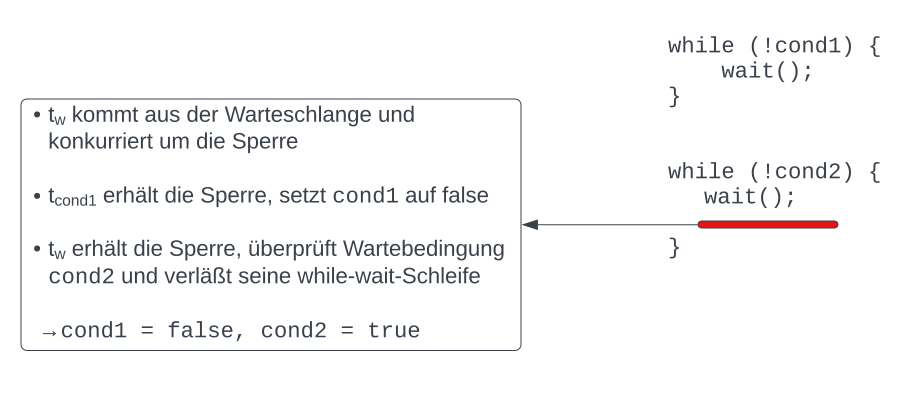
\includegraphics[scale=0.4]{chapters/Anhang/Klausuren/img/cond1cond2}
    \caption{in den rot markierten Bereich konkurriert $t_w$ um die Sperre des Objektes - wenn durch einen anderen Thread, der vor $t_w$ die Sperre erhält, \textit{cond1} auf \textit{false} gesetzt wird, stimmt die Ausgabe nicht mit der erwarteten überein. (Quelle: eigene)}
    \label{fig:cond1cond2}
\end{figure}

\noindent
Die korrekte Wartebedingung sollte lauten:

\begin{minted}[mathescape,
    linenos,
    numbersep=5pt,
    gobble=2,
    fontsize=\small,
    frame=lines,
    framesep=2mm]{java}
    public synchronized void cond1AndCond2() {
        while(!cond1 || !cond2) {
            try {
                wait();
            } catch(InterruptedException e) { }
        }
        System.out.println("cond1 and cond2:" + cond1 + " " + cond2);
    }
\end{minted}\\

Darüber hinaus müßte \code{notifyAll()} nur aufgerufen werden, wenn sowohl \code{cond1} als auch \code{cond2} auf \code{true} gesetzt sind, was leicht in den entsprechenden Methoden überprüft werden kann.
    \chapter{SS19}\label{ch:klausurss19}

\section{Aufgabe 1}

Bei der Aufgabe ist es wichtig, die Anforderungen genau zu beachten.\\
Ob eine Thread die while-wait-Schleife verlassen darf, wird von der Methode \code{tick()} gesteuert - wieviele Ticks ein Thread in der Schleife bleiben soll, wird von dem jeweiligen Thread definiert.\\
Die \code{tick()}-Methode wird von anderen Threads aufgerufen, es kann also durchaus vorkommen, dass mehrmals hintereinander
die \code{notifyAll()}-Methode aufgerufen wird - diese entfernt alle Threads aus der Warteschlange, damit die Threads ihre
Wartebedingungen erneut überprüfen können.\\
da \code{tick()} aber auch gleichzeitig einen Zähler realisieren soll, \textit{muss} es in der Methode auch eine Zählvariable geben, anhand derer die in der while-wait-Schleife enthaltenen Threads feststellen können, wie oft \code{tick()} aufgerufen wurde, um entsprechend aus der Schleife und nachfolgend der Methode herauszukommen.

\begin{figure}
    \centering
    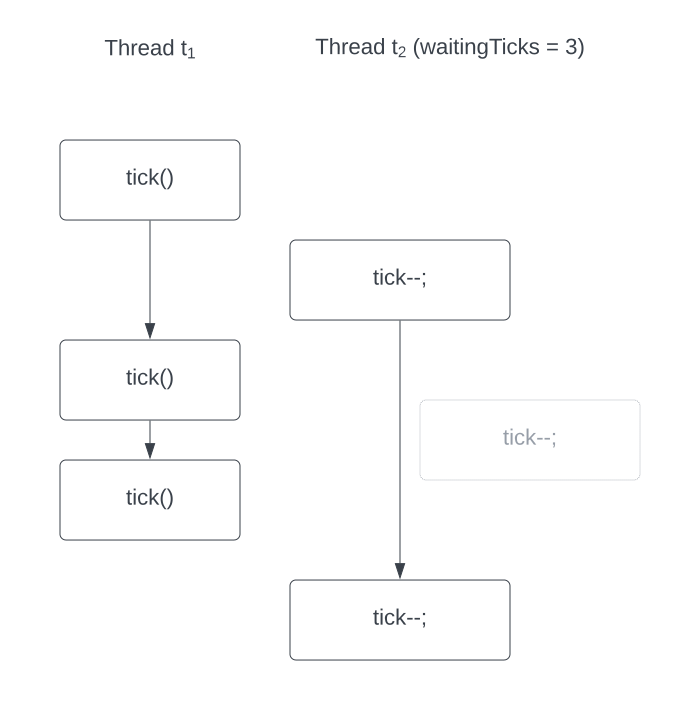
\includegraphics[scale=0.5]{chapters/Anhang/Klausuren/img/tick}
    \caption{Thread $t_1$ ruft 3 mal \texit{tick()} auf. Den Anforderungen nach müsste Thread $t_2$ danach aus der while-wait-Schleife herauskommen, erhält aber nicht die Sperre auf das Objekt von LogicalTime, um seinen eigenen Zähler rechtzeitig zu erniedrigen, bevor $t_1$ erneut \textit{tick()} aufruft. (Quelle: eigene)}
    \label{fig:tick}
\end{figure}

\section{Aufgabe 6}
Auch hier gilt, dass die Aufgabenstellung aufmerksam zu lesen ist.\\
Der Kreis soll erst ausgefüllt werden, wenn die Maustaste gelöst wird.

\begin{minted}[mathescape,
    linenos,
    numbersep=5pt,
    gobble=2,
    frame=lines,
    framesep=2mm]{java}
    private void mousePressed(double x, double y) {
        c = new Circle();
        c.setCenterX(x);
        c.setCenterY(y);
        c.setStroke(Color.RED);
        c.setFill(null); // oder Color.TRANSPARENT
        c.setRadius(RADIUS);
        graphicsPane.getChildren().add(c);
    }

    private void mouseReleased() {
        c.setFill(Color.RED);
        c = null;
    }
\end{minted}

\section{Aufgabe 8}

In der Abbildung \ref{fig:batchmodus} ist links der sequentielle Modus dargestellt, bei dem nach dem Senden einer Nachricht auf die Antwort des Servers gewartet wird, bevor eine neue Nachricht geschickt wird.
Dies wird i.d.R. verwendet, wenn das Senden einer neuen Nachricht abhängig ist von einem Ergebnis, die über die Server-Antwort übermittelt wird, oder wenn mit dem Server interagiert wird (Request abhängig vom Response).\\
Der Batch-Modus auf der rechten Seite der gleichen Abbildung ist schneller, da zwischen dem Senden von Nachrichten nicht auf Antworten gewartet werden müssen. \\
Erst nach dem Senden eine Batches von Nachrichten werden die dem Client zur Verfügung stehenden Antworten ausgelesen.\\

\noindent
In dieser Form des Batch-Modus besteht allerdings die Gefahr, dass es zu Verklemmungen kommt:
\begin{itemize}
    \item Bei dem Client kommen viele Nachrichten an, während er noch sendet.
    \item Die ankommenden Nachrichten für den Client werden gepuffert, bis sie ausgelesen werden (TCP- / OS-seitig).
    \item Läuft der Puffer voll, sorgt die Flusskontrolle (TCP) dafür, dass dem Sender mitgeteilt wird, dass keine Nachrichten mehr empfangen werden können, der Server sendet nicht mehr.
    \item Die zu sendenden Nachrichten des Servers werden in einen Puffer geschrieben.
    \item Der Sende-Puffer des Senders läuft voll.
    \item Bei dem nächsten Sende-Aufruf blockiert der Server, empfangene Nachrichten landen im Empfangspuffer
    \item Der Empfangspuffer des Servers läuft voll, der Client buffert die zu sendenden Nachrichten.
    \item Beide Anwendungen blockieren.
\end{itemize}

\\noindent
Um dieses Problem beim Batch-Modus zu umgehen, werden für das Senden und Empfangen zwei Threads auf Client-Seite erstellt: Ein Thread sendet, ein Thread empfängt. \\
Dadurch kann von dem Client immer wieder sein Empfangspuffer geleert werden, der Server wird beim Senden nicht blockiert.

\begin{figure}
    \centering
    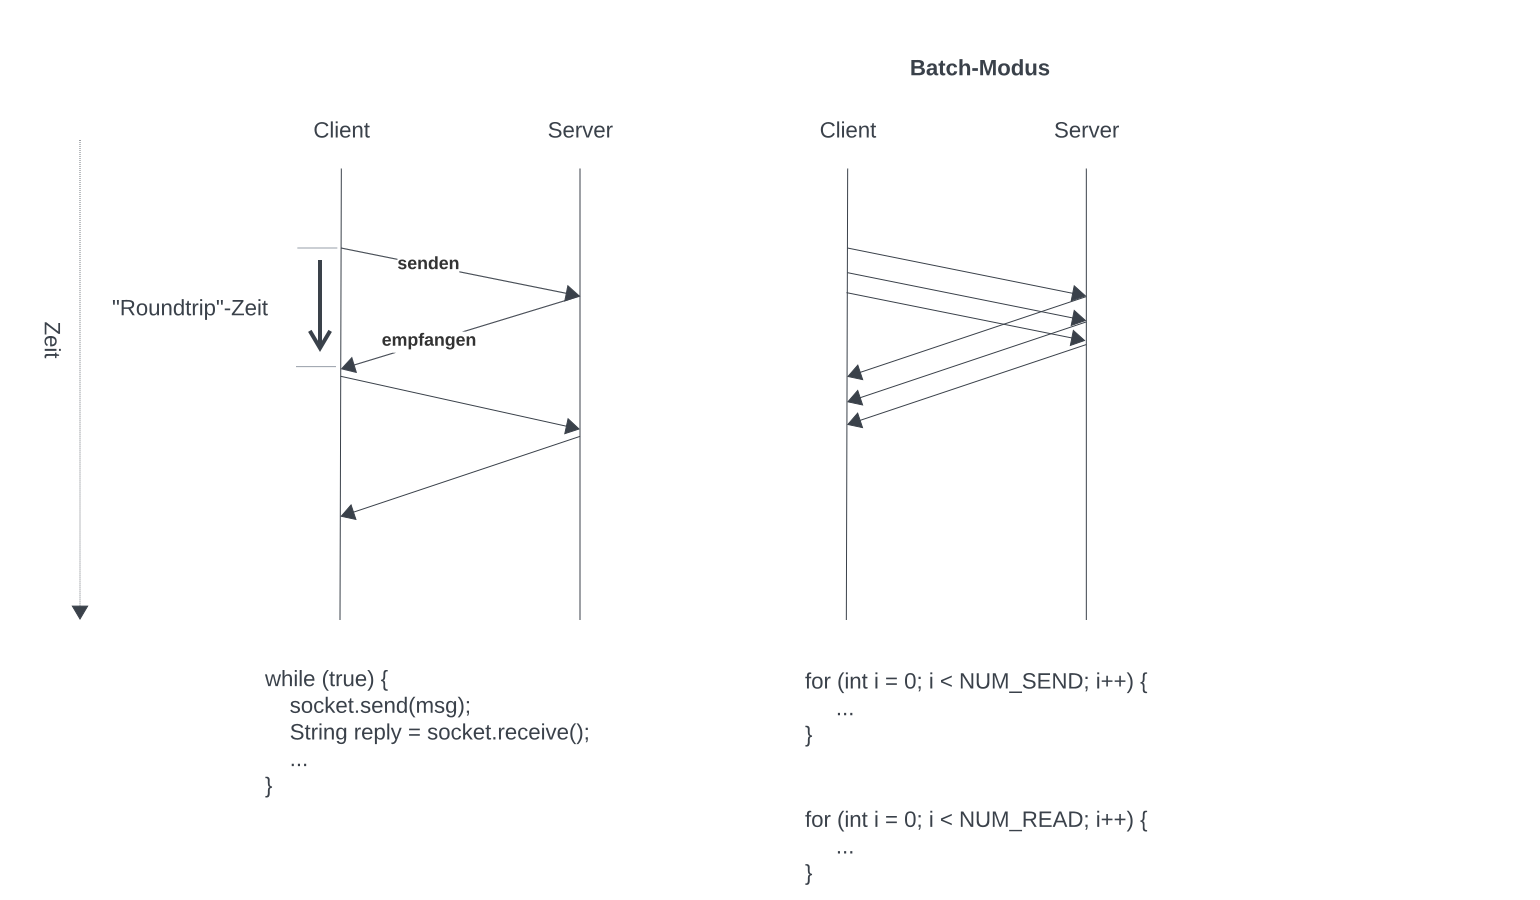
\includegraphics[scale=0.4]{chapters/Anhang/Klausuren/img/batchmodus}
    \caption{Vereinfachte Darstellung sequentieller Kommunikation und Batch-Modus (Quelle: eigene)}
    \label{fig:batchmodus}
\end{figure}
    
\begin{appendices}
    \input{chapters/Anhang/Zusatzaufgaben/index}
    \input{chapters/Anhang/Klausuren/ws13}
    \input{chapters/Anhang/Klausuren/ws15-16}
    \input{chapters/Anhang/Klausuren/ws16-17}
    \input{chapters/Anhang/Klausuren/ss19}
    \input{chapters/Anhang/Präsenzphase/index}

\end{appendices}


\end{appendices}


\end{appendices}


\begin{appendices}
    
\begin{appendices}
    
\begin{appendices}
    \input{chapters/Anhang/Zusatzaufgaben/index}
    \input{chapters/Anhang/Klausuren/ws13}
    \input{chapters/Anhang/Klausuren/ws15-16}
    \input{chapters/Anhang/Klausuren/ws16-17}
    \input{chapters/Anhang/Klausuren/ss19}
    \input{chapters/Anhang/Präsenzphase/index}

\end{appendices}

    \chapter{WS13}\label{ch:klausurws13}

\section{Aufgabe 1}
\subsection{Lösungsvorschlag}


\begin{minted}[mathescape,
    linenos,
    numbersep=5pt,
    gobble=2,
    fontsize=\small,
    frame=lines,
    framesep=2mm]{java}
    class Zahlenschloss {

        private int[] kombination;

        private int[] state;

        private boolean opened = false;

        public Zahlenschloss(int[] kombination) {
            this.kombination = kombination;
            this.state = new int[kombination.length];
        }

        public int anzahlRaedchen() {
            return kombination.length;
        }

        public synchronized int lesen(int radnummer) {
            return state[radnummer];
        }

        public synchronized void drehen(int radnummer, int zahl) {

            state[radnummer] = zahl;
            opened = true;
            for (int i = 0; i < anzahlRaedchen(); i++) {
                if (lesen(i) != kombination[i]) {
                    opened = false;
                    break;
                }
            }

            if (opened) {
                this.notify();
            }
        }

        public synchronized void warten() {

            while (!opened) {
                try {
                    this.wait();
                } catch (InterruptedException ignored) {}
            }
        }
    }
\end{minted}\\


\subsection{Anmerkung und Ergänzungen}

\begin{itemize}
    \item Es wird eine Wartebedingung benötigt, und zwar für die Methode \code{warten()}; ankommende Threads werden
    in die Warteschlange des Zahlenschloss-Objektes geschickt, wenn \code{opened} auf false gesetzt ist, ansonsten
    verlassen diese direkt die Methode wieder.\\
    Die Methode \code{drehen} benötigt keine separate Wartebedingung.
    Es reicht aus, sicherzustellen, dass das Zahlenschloss nicht gleichzeitig von anderen Threads benutzt werden kann:
    Die Methode \code{drehen} ist hierfür synchronisiert, damit das Zahlenschloss {insg.} immer nur eine Zustandsänderung
    erfährt - es sind andere Implementierungen möglich, in denen das Zahlenschloss dann von mehreren Threads gleichzeitig
    genutzt werden darf, wenn sich die Zugriffe anhand der ``Ziel``-\code{radnummer} unterscheiden, {bspw.} durch Mutex-Semaphore,
    die pro Radnummer verwendet werden\footnote{
        der gleichzeitige Zugriff auf unterschiedliche Arrays-Indizes ist erlaubt, s. `´17.4.1. Shared Variables``: \url{https://docs.oracle.com/javase/specs/jls/se21/html/jls-17.html#jls-1.4.1} - abgerufen 14.2.2024
    }.
    \item Es gibt nur eine Wartebedingung, von daher sollte \code{notify()} genügen.\\
    Wenn wir allerdings davon ausgehen, dass mehrere Threads über die Methode \code{warten()} in die Warteschlange des Objektes eingereiht worden sind,  sollte \code{notifyAll()} verwendet werden (siehe hierzu auch Abschnitt \ref{subsec:notifyAll}).
    Dennoch ist nicht garantiert, dass auch alle Threads aus der Warteschlange gelangen, denn es kann sein, dass ein anderer Thread die Methode \code{drehen()} betritt, dort die
    Zahlenkombination ändert und \code{opened} wieder auf \code{false} gesetzt wird. \\
    Ein anderer Thread, der nun in  \code{warten()} an die Reihe kommt, überprüft die Wartebedingung, und wird wieder in die Warteschlange eingereiht.
    Es ist also durchaus möglich, dass ein Thread nicht mehr aus der Methode \code{warten()} herauskommt.\\
    Dies könnte bspw. dadurch verhindert werden, dass die Threads in eine Queue gepackt werden, und in \code{drehen()} eine Wartebedingung eingefügt wird, die erst erfüllt ist,
    wenn die Queue geleert wurde oder aus ihr entnommen wurde, in der Reihenfolge, in der die Threads in die Queue eingereiht worden sind (\textit{FIFO}) (s. a. Abschnitt~\ref{subsec:readerwriterproblem}).
    \item Bei der Teilaufgabe mit der Schleife muss die komplette Schleife synchronisiert werden, was man durch ein \code{synchronized}-Statement erreicht\footnote{siehe Abschnitt~\ref{subsec:synchronizedstatement}.}
    \begin{minted}[mathescape,
        linenos,
        numbersep=5pt,
        gobble=2,
        fontsize=\small,
        frame=lines,
        framesep=2mm]{java}
        synchronized (zk) {
            for (int i = 0; i < anzahlRaedchen; i++) {
                System.out.println(zk.lesen(i));
            }
        }
    \end{minted}
    Ansonsten läuft man Gefahr, dass sich nach Auslesen der 1. Position der Wert von Position 2 geändert hat und dadurch eine
    Zahlenkombination ausgegeben wird, die es nicht gegeben hat:
    \begin{enumerate}
        \item $K\coloneqq[0, 0, 0]$
        \item Position $K_0$ wird ausgelesen und liefert $0$.
        \item Thread ändert $K_0$ zu $1$ $\implies K\coloneqq[1, 0, 0] $.
        \item Thread ändert $K_1$ zu $2$ $\implies K\coloneqq[1, 2, 0] $.
        \item Thread ändert $K_2$ zu $3$ $\implies K\coloneqq[1, 2, 3] $.
        \item Positionen $K_1$ und $K_2$ werden ausgelesen und liefern: $2, 3$
        \item Ausgabe: $0, 2, 3$ - diese Kombination hat es in dem Fall aber tatsächlich nicht gegeben.
    \end{enumerate}
\end{itemize}

\begin{tcolorbox}[colback=red!20,color=white,title=Anmerkung]
    Die Methode \code{lesen()} als \code{synchronized} zu markieren könnte man sich vlt. sparen, wenn man davon ausgeht,
    dass die Methode ohnehin in einem \code{synchronized}-Statement verwendet wird, um alle Rädchen abzulesen.\\
    Mehrere Threads können also nicht parallel auf unterschiedliche Positionen des Feldes zugreifen, wenn die Methode
    synchronisiert ist.\\
    Allerdings ist sowohl das Skript als auch das Buch recht klar, was in dieser Situation geschehen muss (s. Skript Fopt1/2, S. 9, außerdem \cite[31, Abschnitt 2.3.6]{Oec22}): Es muss (in diesem Kurs) immer \code{synchronized} verwendet werden, wenn gleichzeitig
    Daten geschrieben und gleichzeitig diese Daten gelesen werden sollen - und eine andere Implementierung, bei der die
    einzelnen Positionen ``gelocked`` sind, so dass ein gleichzeitiger Zugriff auf unterschiedliche Rädchen möglich ist, war nicht gefordert.\\
    Ggfl. würde in anderen Implementierungen der Einsatz von \code{AtomicReferenceArray}\footnote{s. \cite[157 ff.]{Oec22}
    s. ``Class AtomicReferenceArray<E>``: \url{https://docs.oracle.com/en/java/javase/21/docs/api/java.base/java/util/concurrent/atomic/AtomicReferenceArray.html} - abgerufen 15.2.2024
    } Sinn machen, aber das Lehrmaterial ist bereits sehr eindeutig bzgl. der Verwendung von \code{synchronized}.
\end{tcolorbox}



\section{Aufgabe 3}
\subsection{Lösungsvorschlag}

\subsection*{Statische Parallelität}
Statische Parallelität erlaubt es einem Server, eine \textit{fixe} Anzahl von Verbindungen gleichzeitig zu bedienen.\\
Hierbei wird ein Feld von Threads erstellt, wobei jeder Thread das \code{ServerSocket}-Objekt als Referenz übergeben bekommt.
In der \code{run()}-Methode wird dann über \code{accept()} in einer Endlosschleife auf eingehende Verbindungen gewartet, die dann so lange bedient werden, bis sich ein Client wieder abmeldet (oder eine andere Abbruchbedingung erfüllt ist, wie z.B. ein \code{SocketTimeout}).\\
Das sich ein Client abmeldet, bekommt man bspw. dadurch mit, dass \code{null} beim Lesen von einer Nachricht des Clients zurückgegeben wird (vgl. \cite[286]{Oec22}. \\
Siehe Abschnitt~\ref{sec:seqparserver} für ein Implementierungsbeispiel.



\subsection*{Dynamische Parallelität}

Bei der \textbf{Dynamischer Parallelität} erzeugt der Server für jede Verbindung einen neuen Thread, der so lange läuft, bis der Client die Verbindung wieder trennt.\\
Die Anzahl der Threads ändert sich dadurch laufend.\\
Wird die max. Anzahl erlaubter Threads nicht kontrolliert, kann es zu einer Überlastung des Server-Rechners kommen (bspw. durch einen Denial-of-Service-Angriff.)\\

\noindent
I.d.R. ist eine Mischform aus beidem geeignet, um mehrere Clients gleichzeitig bedienen zu können, und dabei nicht Gefahr zu laufen, durch dynamisches, unbegrenztes Wachstum der Anzahl der Threads überlastet zu werden.

    \chapter{WS13}\label{ch:klausurws5-16}

\section{Rechteck-Scroll (SS15 Aufgabe 2)}

Aufgabenstellung unklar.\\
Mögliche Implementierung unter \url{https://github.com/ThorstenSuckow/fopt/tree/main/src/main/java/klausurvorbereitung/foptws1516/MouseDragsSquareDemo}.

\section{Rechteck-Scroll (WS15/16 Aufgabe 1)}

Aufgabenstellung unklar.\\
Mögliche Implementierung unter \url{https://github.com/ThorstenSuckow/fopt/tree/main/src/main/java/klausurvorbereitung/foptws1516/MaxWeightDemo}.\\

\noindent
Es gibt nur eine Warteschlange für Threads in \code{use()}, es gibt keine Wartebedingung in \code{dontUse()} und damit auch keine weitere Warteschlange.\\
Es sind durch die Zugriffe auf unterschiedliche Indizes allerdings mehrere Wartebedingungen vorhanden, weshalb hab \code{notifyAll()} nutzen sollte,
sobald ein Zugriff auf ein Feld nach Aufruf von \code{dontUse} wieder möglich wird.\\
Ansonsten bestünde die Gefahr, dass bei dem Einsatz von \code{notify()} ein wartender Thread nicht geweckt wird, obwohl er weiterlaufen könnte:\\
Angenommen, das Feld $F$ hat eine Länge von $3$, das \code{maxWeight} ist mit $2$ konfiguriert.
Thread $t_1$ mit einer Laufzeit von $200\ sek$ bekommt Zugriff auf $F_0$, setzt $currentWeight$ auf $1$.\\
Thread $t_2$ mit einer Laufzeit von $1\ sek$ möchte auf $F_1$ zugreifen, setzt $currentWeight=2$ in die Warteschlange.\\
Thread $t_3$ meldet Zugriff auf $F_0$ an und gelangt in die Warteschlange.\\
Thread $t_4$ meldet Zugriff auf $F_1$ an und gelangt in die Warteschlange.\\
Thread $t_2$ ist mit der Bearbeitung von $F_1$ fertig, $currentWeight$ wird auf $1$ gesetzt, \code{notify()} wird aufgerufen.\\
Thread $t_3$ wird aus der Warteschlange geholt, kann aber nicht weiterarbeiten, da $F_0$ noch durch den länger dauernden $t_1$ blockiert ist, und kommt wieder in die Warteschlange.\\

\noindent
Offensichtlich hätte in dem Beispiel \code{notifyAll()} dazu geführt, dass auch $T_4$ seine Wartebedingung hätte überprüfen können, und hätte so Zugriff auf $F_1$ bekommen.
Stattdessen muss nun gewartet werden, bis das nächste \code{notify()} aufgerufen wird, oder ein neu ankommender Thread $F_1$ belegt.

    \chapter{WS16-17}\label{ch:klausurws16-17}

\section{Aufgabe 1}
\subsection{Lösungshinweis}

Die erste Aufgabe verdeutlicht, was bei einem \code{notifyAll()} und unsauber gesetzten Wartebedingungen passieren kann.\\
Sei folgender Quellcode gegeben:


\begin{minted}[mathescape,
    linenos,
    numbersep=5pt,
    gobble=2,
    fontsize=\small,
    frame=lines,
    framesep=2mm]{java}
    class Cond1AndCond2 {

        private boolean cond1;
        private boolean cond2;

        public synchronized void setCond1(boolean c) {
            cond1 = c;
            notifyAll();
        }

        public synchronized void setCond2(boolean c) {
            cond2 = c;
            notifyAll();
        }

        public synchronized void cond1AndCond2() {
            while(!cond1) {
                try {
                    wait();
                } catch(InterruptedException e) { }
            }

            while(!cond2) {
                try {
                    wait();
                } catch(InterruptedException e) {}
            }
            System.out.println("cond1 and cond2:" + cond1 + " " + cond2);
        }
    }
\end{minted}\\

Man sollte auf den ersten Blick meinen, dass \code{cond1} und \code{cond2} beide \code{true} sein müssen, damit die Ausgabe erfolgt.\\
Tatsächlich ist es aber so, dass es in der Methode zwei unterschiedliche Wartebedingungen gibt.\\
Die erste Wartebedingung schickt einen Thread in die Warteschlange, wenn \code{cond1 == false} gilt.\\
Setzt ein anderer Thread über \code{setCond1(true)} das Attribut entsprechend auf \code{true}, bewirkt der nachfolgende Aufruf von \code{notifyAll()}, dass alle \textit{wartenden} Threads aus der Warteschlange entfernt werden und erneut um eine Sperre des Objektes konkurrieren.\\
Erhält ein entsprechender Thread $t_w$ die Sperre auf das Objekt und kann seine \textit{while-wait-Schleife} verlassen, kann es vorkommen, dass er erneut in die Warteschlange eingereiht wird, wegen der nachfolgenden Wartebedingung \code{cond2 == false}.\\
Angenommen, ein weiterer Thread ruft nun \code{setCond2(true)} auf, und $t_w$ kommt aus der Warteschlange und konkurriert erneut und um die Sperre des Objektes, dann kann es vorkommen, das ein anderer Thread zunächst die Sperre erhält, \code{cond1} wieder auf \code{false} setzt, dann erhält $t_w$ die Sperre, überprüft die Wartebedingung \code{cond2 == false}.\\
Wegen \code{cond2} gelangt er aus der \textit{while-wait-Schleife} und die Ausgabe erfolgt - da zwischenzeitlich \code{cond1} wieder auf \code{false} gesetzt wurde, ist die erwartete Ausgabe nicht \code{true true}, sondern \code{false true} (s. Abbildung \ref{fig:cond1cond2}).\\

\begin{figure}
    \centering
    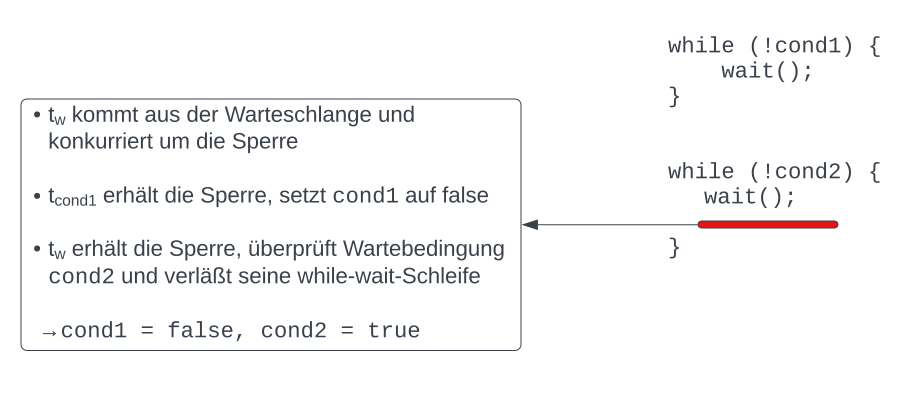
\includegraphics[scale=0.4]{chapters/Anhang/Klausuren/img/cond1cond2}
    \caption{in den rot markierten Bereich konkurriert $t_w$ um die Sperre des Objektes - wenn durch einen anderen Thread, der vor $t_w$ die Sperre erhält, \textit{cond1} auf \textit{false} gesetzt wird, stimmt die Ausgabe nicht mit der erwarteten überein. (Quelle: eigene)}
    \label{fig:cond1cond2}
\end{figure}

\noindent
Die korrekte Wartebedingung sollte lauten:

\begin{minted}[mathescape,
    linenos,
    numbersep=5pt,
    gobble=2,
    fontsize=\small,
    frame=lines,
    framesep=2mm]{java}
    public synchronized void cond1AndCond2() {
        while(!cond1 || !cond2) {
            try {
                wait();
            } catch(InterruptedException e) { }
        }
        System.out.println("cond1 and cond2:" + cond1 + " " + cond2);
    }
\end{minted}\\

Darüber hinaus müßte \code{notifyAll()} nur aufgerufen werden, wenn sowohl \code{cond1} als auch \code{cond2} auf \code{true} gesetzt sind, was leicht in den entsprechenden Methoden überprüft werden kann.
    \chapter{SS19}\label{ch:klausurss19}

\section{Aufgabe 1}

Bei der Aufgabe ist es wichtig, die Anforderungen genau zu beachten.\\
Ob eine Thread die while-wait-Schleife verlassen darf, wird von der Methode \code{tick()} gesteuert - wieviele Ticks ein Thread in der Schleife bleiben soll, wird von dem jeweiligen Thread definiert.\\
Die \code{tick()}-Methode wird von anderen Threads aufgerufen, es kann also durchaus vorkommen, dass mehrmals hintereinander
die \code{notifyAll()}-Methode aufgerufen wird - diese entfernt alle Threads aus der Warteschlange, damit die Threads ihre
Wartebedingungen erneut überprüfen können.\\
da \code{tick()} aber auch gleichzeitig einen Zähler realisieren soll, \textit{muss} es in der Methode auch eine Zählvariable geben, anhand derer die in der while-wait-Schleife enthaltenen Threads feststellen können, wie oft \code{tick()} aufgerufen wurde, um entsprechend aus der Schleife und nachfolgend der Methode herauszukommen.

\begin{figure}
    \centering
    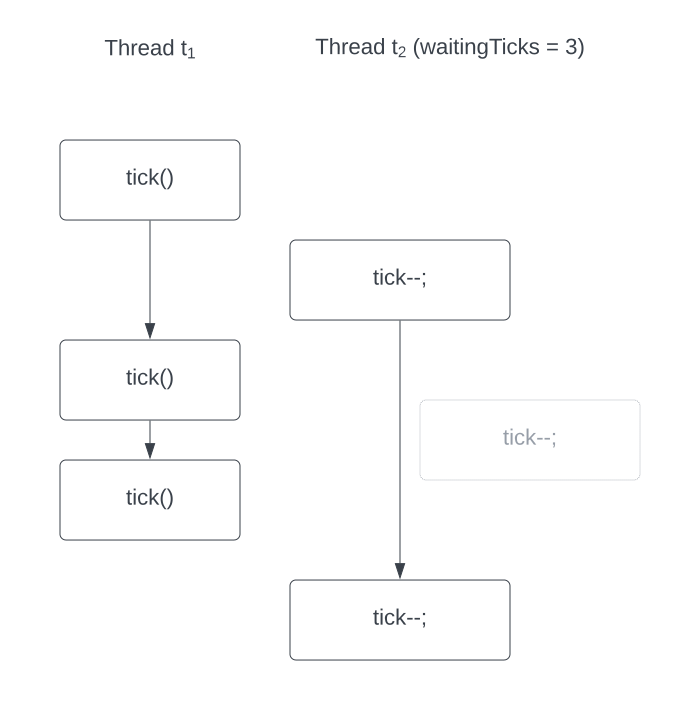
\includegraphics[scale=0.5]{chapters/Anhang/Klausuren/img/tick}
    \caption{Thread $t_1$ ruft 3 mal \texit{tick()} auf. Den Anforderungen nach müsste Thread $t_2$ danach aus der while-wait-Schleife herauskommen, erhält aber nicht die Sperre auf das Objekt von LogicalTime, um seinen eigenen Zähler rechtzeitig zu erniedrigen, bevor $t_1$ erneut \textit{tick()} aufruft. (Quelle: eigene)}
    \label{fig:tick}
\end{figure}

\section{Aufgabe 6}
Auch hier gilt, dass die Aufgabenstellung aufmerksam zu lesen ist.\\
Der Kreis soll erst ausgefüllt werden, wenn die Maustaste gelöst wird.

\begin{minted}[mathescape,
    linenos,
    numbersep=5pt,
    gobble=2,
    frame=lines,
    framesep=2mm]{java}
    private void mousePressed(double x, double y) {
        c = new Circle();
        c.setCenterX(x);
        c.setCenterY(y);
        c.setStroke(Color.RED);
        c.setFill(null); // oder Color.TRANSPARENT
        c.setRadius(RADIUS);
        graphicsPane.getChildren().add(c);
    }

    private void mouseReleased() {
        c.setFill(Color.RED);
        c = null;
    }
\end{minted}

\section{Aufgabe 8}

In der Abbildung \ref{fig:batchmodus} ist links der sequentielle Modus dargestellt, bei dem nach dem Senden einer Nachricht auf die Antwort des Servers gewartet wird, bevor eine neue Nachricht geschickt wird.
Dies wird i.d.R. verwendet, wenn das Senden einer neuen Nachricht abhängig ist von einem Ergebnis, die über die Server-Antwort übermittelt wird, oder wenn mit dem Server interagiert wird (Request abhängig vom Response).\\
Der Batch-Modus auf der rechten Seite der gleichen Abbildung ist schneller, da zwischen dem Senden von Nachrichten nicht auf Antworten gewartet werden müssen. \\
Erst nach dem Senden eine Batches von Nachrichten werden die dem Client zur Verfügung stehenden Antworten ausgelesen.\\

\noindent
In dieser Form des Batch-Modus besteht allerdings die Gefahr, dass es zu Verklemmungen kommt:
\begin{itemize}
    \item Bei dem Client kommen viele Nachrichten an, während er noch sendet.
    \item Die ankommenden Nachrichten für den Client werden gepuffert, bis sie ausgelesen werden (TCP- / OS-seitig).
    \item Läuft der Puffer voll, sorgt die Flusskontrolle (TCP) dafür, dass dem Sender mitgeteilt wird, dass keine Nachrichten mehr empfangen werden können, der Server sendet nicht mehr.
    \item Die zu sendenden Nachrichten des Servers werden in einen Puffer geschrieben.
    \item Der Sende-Puffer des Senders läuft voll.
    \item Bei dem nächsten Sende-Aufruf blockiert der Server, empfangene Nachrichten landen im Empfangspuffer
    \item Der Empfangspuffer des Servers läuft voll, der Client buffert die zu sendenden Nachrichten.
    \item Beide Anwendungen blockieren.
\end{itemize}

\\noindent
Um dieses Problem beim Batch-Modus zu umgehen, werden für das Senden und Empfangen zwei Threads auf Client-Seite erstellt: Ein Thread sendet, ein Thread empfängt. \\
Dadurch kann von dem Client immer wieder sein Empfangspuffer geleert werden, der Server wird beim Senden nicht blockiert.

\begin{figure}
    \centering
    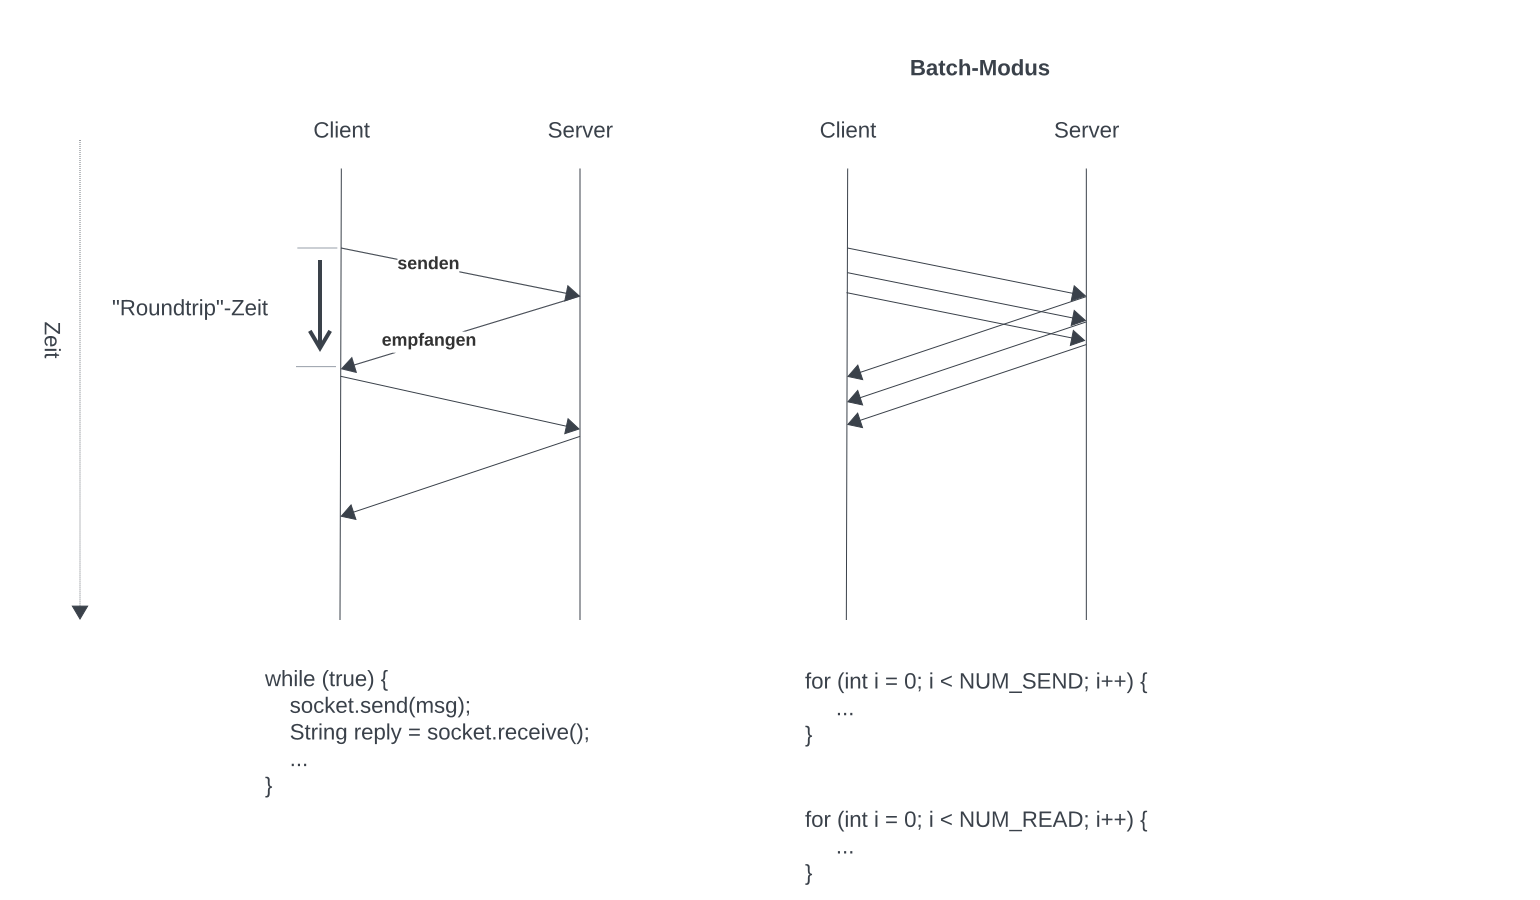
\includegraphics[scale=0.4]{chapters/Anhang/Klausuren/img/batchmodus}
    \caption{Vereinfachte Darstellung sequentieller Kommunikation und Batch-Modus (Quelle: eigene)}
    \label{fig:batchmodus}
\end{figure}
    
\begin{appendices}
    \input{chapters/Anhang/Zusatzaufgaben/index}
    \input{chapters/Anhang/Klausuren/ws13}
    \input{chapters/Anhang/Klausuren/ws15-16}
    \input{chapters/Anhang/Klausuren/ws16-17}
    \input{chapters/Anhang/Klausuren/ss19}
    \input{chapters/Anhang/Präsenzphase/index}

\end{appendices}


\end{appendices}

    \chapter{WS13}\label{ch:klausurws13}

\section{Aufgabe 1}
\subsection{Lösungsvorschlag}


\begin{minted}[mathescape,
    linenos,
    numbersep=5pt,
    gobble=2,
    fontsize=\small,
    frame=lines,
    framesep=2mm]{java}
    class Zahlenschloss {

        private int[] kombination;

        private int[] state;

        private boolean opened = false;

        public Zahlenschloss(int[] kombination) {
            this.kombination = kombination;
            this.state = new int[kombination.length];
        }

        public int anzahlRaedchen() {
            return kombination.length;
        }

        public synchronized int lesen(int radnummer) {
            return state[radnummer];
        }

        public synchronized void drehen(int radnummer, int zahl) {

            state[radnummer] = zahl;
            opened = true;
            for (int i = 0; i < anzahlRaedchen(); i++) {
                if (lesen(i) != kombination[i]) {
                    opened = false;
                    break;
                }
            }

            if (opened) {
                this.notify();
            }
        }

        public synchronized void warten() {

            while (!opened) {
                try {
                    this.wait();
                } catch (InterruptedException ignored) {}
            }
        }
    }
\end{minted}\\


\subsection{Anmerkung und Ergänzungen}

\begin{itemize}
    \item Es wird eine Wartebedingung benötigt, und zwar für die Methode \code{warten()}; ankommende Threads werden
    in die Warteschlange des Zahlenschloss-Objektes geschickt, wenn \code{opened} auf false gesetzt ist, ansonsten
    verlassen diese direkt die Methode wieder.\\
    Die Methode \code{drehen} benötigt keine separate Wartebedingung.
    Es reicht aus, sicherzustellen, dass das Zahlenschloss nicht gleichzeitig von anderen Threads benutzt werden kann:
    Die Methode \code{drehen} ist hierfür synchronisiert, damit das Zahlenschloss {insg.} immer nur eine Zustandsänderung
    erfährt - es sind andere Implementierungen möglich, in denen das Zahlenschloss dann von mehreren Threads gleichzeitig
    genutzt werden darf, wenn sich die Zugriffe anhand der ``Ziel``-\code{radnummer} unterscheiden, {bspw.} durch Mutex-Semaphore,
    die pro Radnummer verwendet werden\footnote{
        der gleichzeitige Zugriff auf unterschiedliche Arrays-Indizes ist erlaubt, s. `´17.4.1. Shared Variables``: \url{https://docs.oracle.com/javase/specs/jls/se21/html/jls-17.html#jls-1.4.1} - abgerufen 14.2.2024
    }.
    \item Es gibt nur eine Wartebedingung, von daher sollte \code{notify()} genügen.\\
    Wenn wir allerdings davon ausgehen, dass mehrere Threads über die Methode \code{warten()} in die Warteschlange des Objektes eingereiht worden sind,  sollte \code{notifyAll()} verwendet werden (siehe hierzu auch Abschnitt \ref{subsec:notifyAll}).
    Dennoch ist nicht garantiert, dass auch alle Threads aus der Warteschlange gelangen, denn es kann sein, dass ein anderer Thread die Methode \code{drehen()} betritt, dort die
    Zahlenkombination ändert und \code{opened} wieder auf \code{false} gesetzt wird. \\
    Ein anderer Thread, der nun in  \code{warten()} an die Reihe kommt, überprüft die Wartebedingung, und wird wieder in die Warteschlange eingereiht.
    Es ist also durchaus möglich, dass ein Thread nicht mehr aus der Methode \code{warten()} herauskommt.\\
    Dies könnte bspw. dadurch verhindert werden, dass die Threads in eine Queue gepackt werden, und in \code{drehen()} eine Wartebedingung eingefügt wird, die erst erfüllt ist,
    wenn die Queue geleert wurde oder aus ihr entnommen wurde, in der Reihenfolge, in der die Threads in die Queue eingereiht worden sind (\textit{FIFO}) (s. a. Abschnitt~\ref{subsec:readerwriterproblem}).
    \item Bei der Teilaufgabe mit der Schleife muss die komplette Schleife synchronisiert werden, was man durch ein \code{synchronized}-Statement erreicht\footnote{siehe Abschnitt~\ref{subsec:synchronizedstatement}.}
    \begin{minted}[mathescape,
        linenos,
        numbersep=5pt,
        gobble=2,
        fontsize=\small,
        frame=lines,
        framesep=2mm]{java}
        synchronized (zk) {
            for (int i = 0; i < anzahlRaedchen; i++) {
                System.out.println(zk.lesen(i));
            }
        }
    \end{minted}
    Ansonsten läuft man Gefahr, dass sich nach Auslesen der 1. Position der Wert von Position 2 geändert hat und dadurch eine
    Zahlenkombination ausgegeben wird, die es nicht gegeben hat:
    \begin{enumerate}
        \item $K\coloneqq[0, 0, 0]$
        \item Position $K_0$ wird ausgelesen und liefert $0$.
        \item Thread ändert $K_0$ zu $1$ $\implies K\coloneqq[1, 0, 0] $.
        \item Thread ändert $K_1$ zu $2$ $\implies K\coloneqq[1, 2, 0] $.
        \item Thread ändert $K_2$ zu $3$ $\implies K\coloneqq[1, 2, 3] $.
        \item Positionen $K_1$ und $K_2$ werden ausgelesen und liefern: $2, 3$
        \item Ausgabe: $0, 2, 3$ - diese Kombination hat es in dem Fall aber tatsächlich nicht gegeben.
    \end{enumerate}
\end{itemize}

\begin{tcolorbox}[colback=red!20,color=white,title=Anmerkung]
    Die Methode \code{lesen()} als \code{synchronized} zu markieren könnte man sich vlt. sparen, wenn man davon ausgeht,
    dass die Methode ohnehin in einem \code{synchronized}-Statement verwendet wird, um alle Rädchen abzulesen.\\
    Mehrere Threads können also nicht parallel auf unterschiedliche Positionen des Feldes zugreifen, wenn die Methode
    synchronisiert ist.\\
    Allerdings ist sowohl das Skript als auch das Buch recht klar, was in dieser Situation geschehen muss (s. Skript Fopt1/2, S. 9, außerdem \cite[31, Abschnitt 2.3.6]{Oec22}): Es muss (in diesem Kurs) immer \code{synchronized} verwendet werden, wenn gleichzeitig
    Daten geschrieben und gleichzeitig diese Daten gelesen werden sollen - und eine andere Implementierung, bei der die
    einzelnen Positionen ``gelocked`` sind, so dass ein gleichzeitiger Zugriff auf unterschiedliche Rädchen möglich ist, war nicht gefordert.\\
    Ggfl. würde in anderen Implementierungen der Einsatz von \code{AtomicReferenceArray}\footnote{s. \cite[157 ff.]{Oec22}
    s. ``Class AtomicReferenceArray<E>``: \url{https://docs.oracle.com/en/java/javase/21/docs/api/java.base/java/util/concurrent/atomic/AtomicReferenceArray.html} - abgerufen 15.2.2024
    } Sinn machen, aber das Lehrmaterial ist bereits sehr eindeutig bzgl. der Verwendung von \code{synchronized}.
\end{tcolorbox}



\section{Aufgabe 3}
\subsection{Lösungsvorschlag}

\subsection*{Statische Parallelität}
Statische Parallelität erlaubt es einem Server, eine \textit{fixe} Anzahl von Verbindungen gleichzeitig zu bedienen.\\
Hierbei wird ein Feld von Threads erstellt, wobei jeder Thread das \code{ServerSocket}-Objekt als Referenz übergeben bekommt.
In der \code{run()}-Methode wird dann über \code{accept()} in einer Endlosschleife auf eingehende Verbindungen gewartet, die dann so lange bedient werden, bis sich ein Client wieder abmeldet (oder eine andere Abbruchbedingung erfüllt ist, wie z.B. ein \code{SocketTimeout}).\\
Das sich ein Client abmeldet, bekommt man bspw. dadurch mit, dass \code{null} beim Lesen von einer Nachricht des Clients zurückgegeben wird (vgl. \cite[286]{Oec22}. \\
Siehe Abschnitt~\ref{sec:seqparserver} für ein Implementierungsbeispiel.



\subsection*{Dynamische Parallelität}

Bei der \textbf{Dynamischer Parallelität} erzeugt der Server für jede Verbindung einen neuen Thread, der so lange läuft, bis der Client die Verbindung wieder trennt.\\
Die Anzahl der Threads ändert sich dadurch laufend.\\
Wird die max. Anzahl erlaubter Threads nicht kontrolliert, kann es zu einer Überlastung des Server-Rechners kommen (bspw. durch einen Denial-of-Service-Angriff.)\\

\noindent
I.d.R. ist eine Mischform aus beidem geeignet, um mehrere Clients gleichzeitig bedienen zu können, und dabei nicht Gefahr zu laufen, durch dynamisches, unbegrenztes Wachstum der Anzahl der Threads überlastet zu werden.

    \chapter{WS13}\label{ch:klausurws5-16}

\section{Rechteck-Scroll (SS15 Aufgabe 2)}

Aufgabenstellung unklar.\\
Mögliche Implementierung unter \url{https://github.com/ThorstenSuckow/fopt/tree/main/src/main/java/klausurvorbereitung/foptws1516/MouseDragsSquareDemo}.

\section{Rechteck-Scroll (WS15/16 Aufgabe 1)}

Aufgabenstellung unklar.\\
Mögliche Implementierung unter \url{https://github.com/ThorstenSuckow/fopt/tree/main/src/main/java/klausurvorbereitung/foptws1516/MaxWeightDemo}.\\

\noindent
Es gibt nur eine Warteschlange für Threads in \code{use()}, es gibt keine Wartebedingung in \code{dontUse()} und damit auch keine weitere Warteschlange.\\
Es sind durch die Zugriffe auf unterschiedliche Indizes allerdings mehrere Wartebedingungen vorhanden, weshalb hab \code{notifyAll()} nutzen sollte,
sobald ein Zugriff auf ein Feld nach Aufruf von \code{dontUse} wieder möglich wird.\\
Ansonsten bestünde die Gefahr, dass bei dem Einsatz von \code{notify()} ein wartender Thread nicht geweckt wird, obwohl er weiterlaufen könnte:\\
Angenommen, das Feld $F$ hat eine Länge von $3$, das \code{maxWeight} ist mit $2$ konfiguriert.
Thread $t_1$ mit einer Laufzeit von $200\ sek$ bekommt Zugriff auf $F_0$, setzt $currentWeight$ auf $1$.\\
Thread $t_2$ mit einer Laufzeit von $1\ sek$ möchte auf $F_1$ zugreifen, setzt $currentWeight=2$ in die Warteschlange.\\
Thread $t_3$ meldet Zugriff auf $F_0$ an und gelangt in die Warteschlange.\\
Thread $t_4$ meldet Zugriff auf $F_1$ an und gelangt in die Warteschlange.\\
Thread $t_2$ ist mit der Bearbeitung von $F_1$ fertig, $currentWeight$ wird auf $1$ gesetzt, \code{notify()} wird aufgerufen.\\
Thread $t_3$ wird aus der Warteschlange geholt, kann aber nicht weiterarbeiten, da $F_0$ noch durch den länger dauernden $t_1$ blockiert ist, und kommt wieder in die Warteschlange.\\

\noindent
Offensichtlich hätte in dem Beispiel \code{notifyAll()} dazu geführt, dass auch $T_4$ seine Wartebedingung hätte überprüfen können, und hätte so Zugriff auf $F_1$ bekommen.
Stattdessen muss nun gewartet werden, bis das nächste \code{notify()} aufgerufen wird, oder ein neu ankommender Thread $F_1$ belegt.

    \chapter{WS16-17}\label{ch:klausurws16-17}

\section{Aufgabe 1}
\subsection{Lösungshinweis}

Die erste Aufgabe verdeutlicht, was bei einem \code{notifyAll()} und unsauber gesetzten Wartebedingungen passieren kann.\\
Sei folgender Quellcode gegeben:


\begin{minted}[mathescape,
    linenos,
    numbersep=5pt,
    gobble=2,
    fontsize=\small,
    frame=lines,
    framesep=2mm]{java}
    class Cond1AndCond2 {

        private boolean cond1;
        private boolean cond2;

        public synchronized void setCond1(boolean c) {
            cond1 = c;
            notifyAll();
        }

        public synchronized void setCond2(boolean c) {
            cond2 = c;
            notifyAll();
        }

        public synchronized void cond1AndCond2() {
            while(!cond1) {
                try {
                    wait();
                } catch(InterruptedException e) { }
            }

            while(!cond2) {
                try {
                    wait();
                } catch(InterruptedException e) {}
            }
            System.out.println("cond1 and cond2:" + cond1 + " " + cond2);
        }
    }
\end{minted}\\

Man sollte auf den ersten Blick meinen, dass \code{cond1} und \code{cond2} beide \code{true} sein müssen, damit die Ausgabe erfolgt.\\
Tatsächlich ist es aber so, dass es in der Methode zwei unterschiedliche Wartebedingungen gibt.\\
Die erste Wartebedingung schickt einen Thread in die Warteschlange, wenn \code{cond1 == false} gilt.\\
Setzt ein anderer Thread über \code{setCond1(true)} das Attribut entsprechend auf \code{true}, bewirkt der nachfolgende Aufruf von \code{notifyAll()}, dass alle \textit{wartenden} Threads aus der Warteschlange entfernt werden und erneut um eine Sperre des Objektes konkurrieren.\\
Erhält ein entsprechender Thread $t_w$ die Sperre auf das Objekt und kann seine \textit{while-wait-Schleife} verlassen, kann es vorkommen, dass er erneut in die Warteschlange eingereiht wird, wegen der nachfolgenden Wartebedingung \code{cond2 == false}.\\
Angenommen, ein weiterer Thread ruft nun \code{setCond2(true)} auf, und $t_w$ kommt aus der Warteschlange und konkurriert erneut und um die Sperre des Objektes, dann kann es vorkommen, das ein anderer Thread zunächst die Sperre erhält, \code{cond1} wieder auf \code{false} setzt, dann erhält $t_w$ die Sperre, überprüft die Wartebedingung \code{cond2 == false}.\\
Wegen \code{cond2} gelangt er aus der \textit{while-wait-Schleife} und die Ausgabe erfolgt - da zwischenzeitlich \code{cond1} wieder auf \code{false} gesetzt wurde, ist die erwartete Ausgabe nicht \code{true true}, sondern \code{false true} (s. Abbildung \ref{fig:cond1cond2}).\\

\begin{figure}
    \centering
    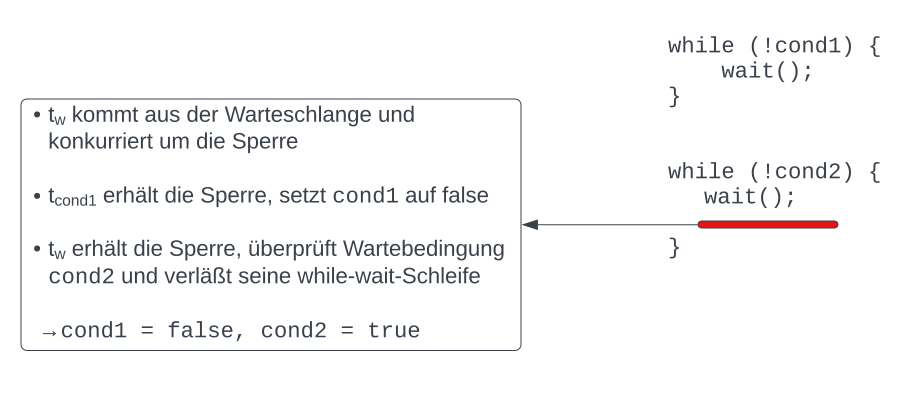
\includegraphics[scale=0.4]{chapters/Anhang/Klausuren/img/cond1cond2}
    \caption{in den rot markierten Bereich konkurriert $t_w$ um die Sperre des Objektes - wenn durch einen anderen Thread, der vor $t_w$ die Sperre erhält, \textit{cond1} auf \textit{false} gesetzt wird, stimmt die Ausgabe nicht mit der erwarteten überein. (Quelle: eigene)}
    \label{fig:cond1cond2}
\end{figure}

\noindent
Die korrekte Wartebedingung sollte lauten:

\begin{minted}[mathescape,
    linenos,
    numbersep=5pt,
    gobble=2,
    fontsize=\small,
    frame=lines,
    framesep=2mm]{java}
    public synchronized void cond1AndCond2() {
        while(!cond1 || !cond2) {
            try {
                wait();
            } catch(InterruptedException e) { }
        }
        System.out.println("cond1 and cond2:" + cond1 + " " + cond2);
    }
\end{minted}\\

Darüber hinaus müßte \code{notifyAll()} nur aufgerufen werden, wenn sowohl \code{cond1} als auch \code{cond2} auf \code{true} gesetzt sind, was leicht in den entsprechenden Methoden überprüft werden kann.
    \chapter{SS19}\label{ch:klausurss19}

\section{Aufgabe 1}

Bei der Aufgabe ist es wichtig, die Anforderungen genau zu beachten.\\
Ob eine Thread die while-wait-Schleife verlassen darf, wird von der Methode \code{tick()} gesteuert - wieviele Ticks ein Thread in der Schleife bleiben soll, wird von dem jeweiligen Thread definiert.\\
Die \code{tick()}-Methode wird von anderen Threads aufgerufen, es kann also durchaus vorkommen, dass mehrmals hintereinander
die \code{notifyAll()}-Methode aufgerufen wird - diese entfernt alle Threads aus der Warteschlange, damit die Threads ihre
Wartebedingungen erneut überprüfen können.\\
da \code{tick()} aber auch gleichzeitig einen Zähler realisieren soll, \textit{muss} es in der Methode auch eine Zählvariable geben, anhand derer die in der while-wait-Schleife enthaltenen Threads feststellen können, wie oft \code{tick()} aufgerufen wurde, um entsprechend aus der Schleife und nachfolgend der Methode herauszukommen.

\begin{figure}
    \centering
    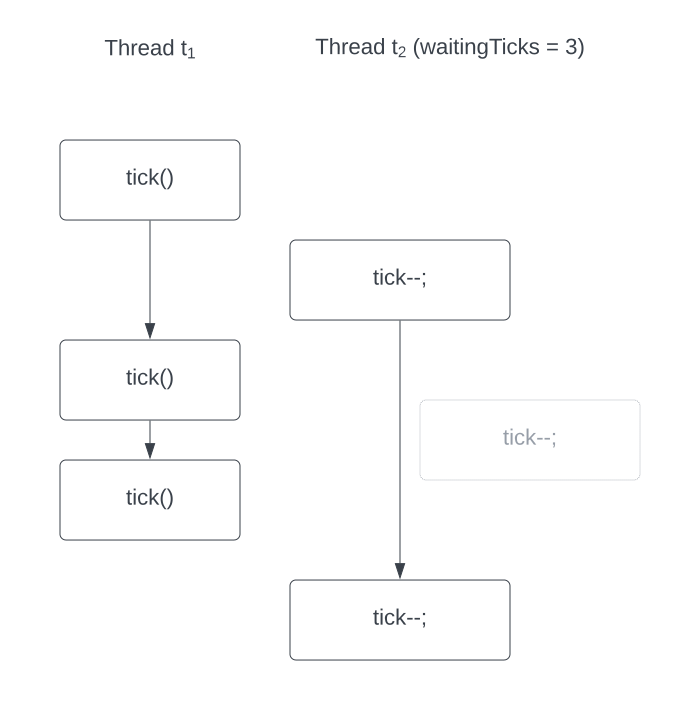
\includegraphics[scale=0.5]{chapters/Anhang/Klausuren/img/tick}
    \caption{Thread $t_1$ ruft 3 mal \texit{tick()} auf. Den Anforderungen nach müsste Thread $t_2$ danach aus der while-wait-Schleife herauskommen, erhält aber nicht die Sperre auf das Objekt von LogicalTime, um seinen eigenen Zähler rechtzeitig zu erniedrigen, bevor $t_1$ erneut \textit{tick()} aufruft. (Quelle: eigene)}
    \label{fig:tick}
\end{figure}

\section{Aufgabe 6}
Auch hier gilt, dass die Aufgabenstellung aufmerksam zu lesen ist.\\
Der Kreis soll erst ausgefüllt werden, wenn die Maustaste gelöst wird.

\begin{minted}[mathescape,
    linenos,
    numbersep=5pt,
    gobble=2,
    frame=lines,
    framesep=2mm]{java}
    private void mousePressed(double x, double y) {
        c = new Circle();
        c.setCenterX(x);
        c.setCenterY(y);
        c.setStroke(Color.RED);
        c.setFill(null); // oder Color.TRANSPARENT
        c.setRadius(RADIUS);
        graphicsPane.getChildren().add(c);
    }

    private void mouseReleased() {
        c.setFill(Color.RED);
        c = null;
    }
\end{minted}

\section{Aufgabe 8}

In der Abbildung \ref{fig:batchmodus} ist links der sequentielle Modus dargestellt, bei dem nach dem Senden einer Nachricht auf die Antwort des Servers gewartet wird, bevor eine neue Nachricht geschickt wird.
Dies wird i.d.R. verwendet, wenn das Senden einer neuen Nachricht abhängig ist von einem Ergebnis, die über die Server-Antwort übermittelt wird, oder wenn mit dem Server interagiert wird (Request abhängig vom Response).\\
Der Batch-Modus auf der rechten Seite der gleichen Abbildung ist schneller, da zwischen dem Senden von Nachrichten nicht auf Antworten gewartet werden müssen. \\
Erst nach dem Senden eine Batches von Nachrichten werden die dem Client zur Verfügung stehenden Antworten ausgelesen.\\

\noindent
In dieser Form des Batch-Modus besteht allerdings die Gefahr, dass es zu Verklemmungen kommt:
\begin{itemize}
    \item Bei dem Client kommen viele Nachrichten an, während er noch sendet.
    \item Die ankommenden Nachrichten für den Client werden gepuffert, bis sie ausgelesen werden (TCP- / OS-seitig).
    \item Läuft der Puffer voll, sorgt die Flusskontrolle (TCP) dafür, dass dem Sender mitgeteilt wird, dass keine Nachrichten mehr empfangen werden können, der Server sendet nicht mehr.
    \item Die zu sendenden Nachrichten des Servers werden in einen Puffer geschrieben.
    \item Der Sende-Puffer des Senders läuft voll.
    \item Bei dem nächsten Sende-Aufruf blockiert der Server, empfangene Nachrichten landen im Empfangspuffer
    \item Der Empfangspuffer des Servers läuft voll, der Client buffert die zu sendenden Nachrichten.
    \item Beide Anwendungen blockieren.
\end{itemize}

\\noindent
Um dieses Problem beim Batch-Modus zu umgehen, werden für das Senden und Empfangen zwei Threads auf Client-Seite erstellt: Ein Thread sendet, ein Thread empfängt. \\
Dadurch kann von dem Client immer wieder sein Empfangspuffer geleert werden, der Server wird beim Senden nicht blockiert.

\begin{figure}
    \centering
    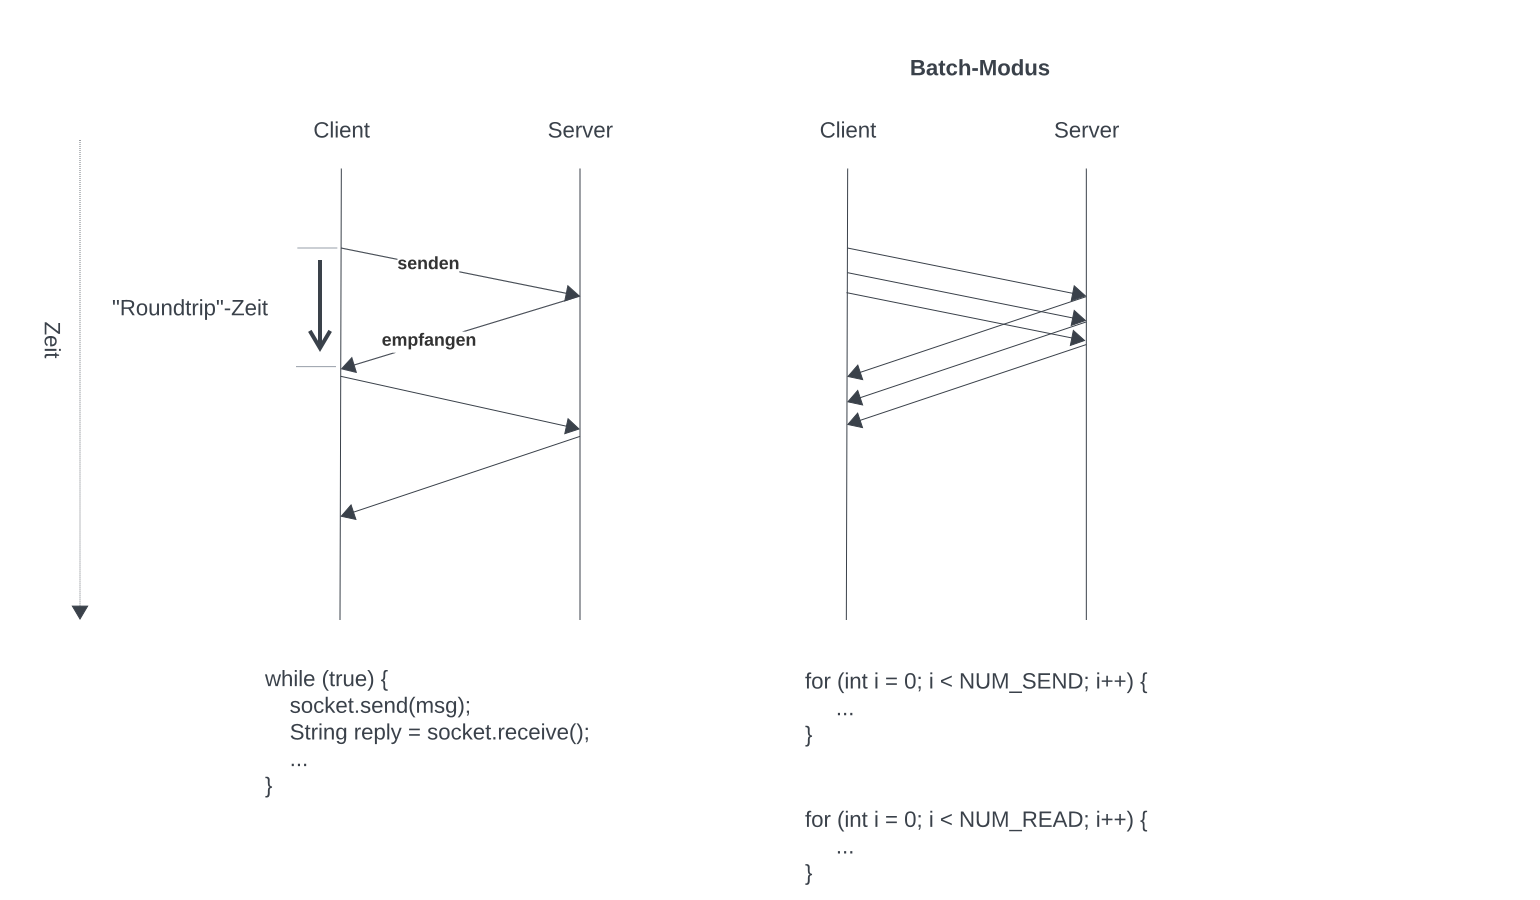
\includegraphics[scale=0.4]{chapters/Anhang/Klausuren/img/batchmodus}
    \caption{Vereinfachte Darstellung sequentieller Kommunikation und Batch-Modus (Quelle: eigene)}
    \label{fig:batchmodus}
\end{figure}
    
\begin{appendices}
    
\begin{appendices}
    \input{chapters/Anhang/Zusatzaufgaben/index}
    \input{chapters/Anhang/Klausuren/ws13}
    \input{chapters/Anhang/Klausuren/ws15-16}
    \input{chapters/Anhang/Klausuren/ws16-17}
    \input{chapters/Anhang/Klausuren/ss19}
    \input{chapters/Anhang/Präsenzphase/index}

\end{appendices}

    \chapter{WS13}\label{ch:klausurws13}

\section{Aufgabe 1}
\subsection{Lösungsvorschlag}


\begin{minted}[mathescape,
    linenos,
    numbersep=5pt,
    gobble=2,
    fontsize=\small,
    frame=lines,
    framesep=2mm]{java}
    class Zahlenschloss {

        private int[] kombination;

        private int[] state;

        private boolean opened = false;

        public Zahlenschloss(int[] kombination) {
            this.kombination = kombination;
            this.state = new int[kombination.length];
        }

        public int anzahlRaedchen() {
            return kombination.length;
        }

        public synchronized int lesen(int radnummer) {
            return state[radnummer];
        }

        public synchronized void drehen(int radnummer, int zahl) {

            state[radnummer] = zahl;
            opened = true;
            for (int i = 0; i < anzahlRaedchen(); i++) {
                if (lesen(i) != kombination[i]) {
                    opened = false;
                    break;
                }
            }

            if (opened) {
                this.notify();
            }
        }

        public synchronized void warten() {

            while (!opened) {
                try {
                    this.wait();
                } catch (InterruptedException ignored) {}
            }
        }
    }
\end{minted}\\


\subsection{Anmerkung und Ergänzungen}

\begin{itemize}
    \item Es wird eine Wartebedingung benötigt, und zwar für die Methode \code{warten()}; ankommende Threads werden
    in die Warteschlange des Zahlenschloss-Objektes geschickt, wenn \code{opened} auf false gesetzt ist, ansonsten
    verlassen diese direkt die Methode wieder.\\
    Die Methode \code{drehen} benötigt keine separate Wartebedingung.
    Es reicht aus, sicherzustellen, dass das Zahlenschloss nicht gleichzeitig von anderen Threads benutzt werden kann:
    Die Methode \code{drehen} ist hierfür synchronisiert, damit das Zahlenschloss {insg.} immer nur eine Zustandsänderung
    erfährt - es sind andere Implementierungen möglich, in denen das Zahlenschloss dann von mehreren Threads gleichzeitig
    genutzt werden darf, wenn sich die Zugriffe anhand der ``Ziel``-\code{radnummer} unterscheiden, {bspw.} durch Mutex-Semaphore,
    die pro Radnummer verwendet werden\footnote{
        der gleichzeitige Zugriff auf unterschiedliche Arrays-Indizes ist erlaubt, s. `´17.4.1. Shared Variables``: \url{https://docs.oracle.com/javase/specs/jls/se21/html/jls-17.html#jls-1.4.1} - abgerufen 14.2.2024
    }.
    \item Es gibt nur eine Wartebedingung, von daher sollte \code{notify()} genügen.\\
    Wenn wir allerdings davon ausgehen, dass mehrere Threads über die Methode \code{warten()} in die Warteschlange des Objektes eingereiht worden sind,  sollte \code{notifyAll()} verwendet werden (siehe hierzu auch Abschnitt \ref{subsec:notifyAll}).
    Dennoch ist nicht garantiert, dass auch alle Threads aus der Warteschlange gelangen, denn es kann sein, dass ein anderer Thread die Methode \code{drehen()} betritt, dort die
    Zahlenkombination ändert und \code{opened} wieder auf \code{false} gesetzt wird. \\
    Ein anderer Thread, der nun in  \code{warten()} an die Reihe kommt, überprüft die Wartebedingung, und wird wieder in die Warteschlange eingereiht.
    Es ist also durchaus möglich, dass ein Thread nicht mehr aus der Methode \code{warten()} herauskommt.\\
    Dies könnte bspw. dadurch verhindert werden, dass die Threads in eine Queue gepackt werden, und in \code{drehen()} eine Wartebedingung eingefügt wird, die erst erfüllt ist,
    wenn die Queue geleert wurde oder aus ihr entnommen wurde, in der Reihenfolge, in der die Threads in die Queue eingereiht worden sind (\textit{FIFO}) (s. a. Abschnitt~\ref{subsec:readerwriterproblem}).
    \item Bei der Teilaufgabe mit der Schleife muss die komplette Schleife synchronisiert werden, was man durch ein \code{synchronized}-Statement erreicht\footnote{siehe Abschnitt~\ref{subsec:synchronizedstatement}.}
    \begin{minted}[mathescape,
        linenos,
        numbersep=5pt,
        gobble=2,
        fontsize=\small,
        frame=lines,
        framesep=2mm]{java}
        synchronized (zk) {
            for (int i = 0; i < anzahlRaedchen; i++) {
                System.out.println(zk.lesen(i));
            }
        }
    \end{minted}
    Ansonsten läuft man Gefahr, dass sich nach Auslesen der 1. Position der Wert von Position 2 geändert hat und dadurch eine
    Zahlenkombination ausgegeben wird, die es nicht gegeben hat:
    \begin{enumerate}
        \item $K\coloneqq[0, 0, 0]$
        \item Position $K_0$ wird ausgelesen und liefert $0$.
        \item Thread ändert $K_0$ zu $1$ $\implies K\coloneqq[1, 0, 0] $.
        \item Thread ändert $K_1$ zu $2$ $\implies K\coloneqq[1, 2, 0] $.
        \item Thread ändert $K_2$ zu $3$ $\implies K\coloneqq[1, 2, 3] $.
        \item Positionen $K_1$ und $K_2$ werden ausgelesen und liefern: $2, 3$
        \item Ausgabe: $0, 2, 3$ - diese Kombination hat es in dem Fall aber tatsächlich nicht gegeben.
    \end{enumerate}
\end{itemize}

\begin{tcolorbox}[colback=red!20,color=white,title=Anmerkung]
    Die Methode \code{lesen()} als \code{synchronized} zu markieren könnte man sich vlt. sparen, wenn man davon ausgeht,
    dass die Methode ohnehin in einem \code{synchronized}-Statement verwendet wird, um alle Rädchen abzulesen.\\
    Mehrere Threads können also nicht parallel auf unterschiedliche Positionen des Feldes zugreifen, wenn die Methode
    synchronisiert ist.\\
    Allerdings ist sowohl das Skript als auch das Buch recht klar, was in dieser Situation geschehen muss (s. Skript Fopt1/2, S. 9, außerdem \cite[31, Abschnitt 2.3.6]{Oec22}): Es muss (in diesem Kurs) immer \code{synchronized} verwendet werden, wenn gleichzeitig
    Daten geschrieben und gleichzeitig diese Daten gelesen werden sollen - und eine andere Implementierung, bei der die
    einzelnen Positionen ``gelocked`` sind, so dass ein gleichzeitiger Zugriff auf unterschiedliche Rädchen möglich ist, war nicht gefordert.\\
    Ggfl. würde in anderen Implementierungen der Einsatz von \code{AtomicReferenceArray}\footnote{s. \cite[157 ff.]{Oec22}
    s. ``Class AtomicReferenceArray<E>``: \url{https://docs.oracle.com/en/java/javase/21/docs/api/java.base/java/util/concurrent/atomic/AtomicReferenceArray.html} - abgerufen 15.2.2024
    } Sinn machen, aber das Lehrmaterial ist bereits sehr eindeutig bzgl. der Verwendung von \code{synchronized}.
\end{tcolorbox}



\section{Aufgabe 3}
\subsection{Lösungsvorschlag}

\subsection*{Statische Parallelität}
Statische Parallelität erlaubt es einem Server, eine \textit{fixe} Anzahl von Verbindungen gleichzeitig zu bedienen.\\
Hierbei wird ein Feld von Threads erstellt, wobei jeder Thread das \code{ServerSocket}-Objekt als Referenz übergeben bekommt.
In der \code{run()}-Methode wird dann über \code{accept()} in einer Endlosschleife auf eingehende Verbindungen gewartet, die dann so lange bedient werden, bis sich ein Client wieder abmeldet (oder eine andere Abbruchbedingung erfüllt ist, wie z.B. ein \code{SocketTimeout}).\\
Das sich ein Client abmeldet, bekommt man bspw. dadurch mit, dass \code{null} beim Lesen von einer Nachricht des Clients zurückgegeben wird (vgl. \cite[286]{Oec22}. \\
Siehe Abschnitt~\ref{sec:seqparserver} für ein Implementierungsbeispiel.



\subsection*{Dynamische Parallelität}

Bei der \textbf{Dynamischer Parallelität} erzeugt der Server für jede Verbindung einen neuen Thread, der so lange läuft, bis der Client die Verbindung wieder trennt.\\
Die Anzahl der Threads ändert sich dadurch laufend.\\
Wird die max. Anzahl erlaubter Threads nicht kontrolliert, kann es zu einer Überlastung des Server-Rechners kommen (bspw. durch einen Denial-of-Service-Angriff.)\\

\noindent
I.d.R. ist eine Mischform aus beidem geeignet, um mehrere Clients gleichzeitig bedienen zu können, und dabei nicht Gefahr zu laufen, durch dynamisches, unbegrenztes Wachstum der Anzahl der Threads überlastet zu werden.

    \chapter{WS13}\label{ch:klausurws5-16}

\section{Rechteck-Scroll (SS15 Aufgabe 2)}

Aufgabenstellung unklar.\\
Mögliche Implementierung unter \url{https://github.com/ThorstenSuckow/fopt/tree/main/src/main/java/klausurvorbereitung/foptws1516/MouseDragsSquareDemo}.

\section{Rechteck-Scroll (WS15/16 Aufgabe 1)}

Aufgabenstellung unklar.\\
Mögliche Implementierung unter \url{https://github.com/ThorstenSuckow/fopt/tree/main/src/main/java/klausurvorbereitung/foptws1516/MaxWeightDemo}.\\

\noindent
Es gibt nur eine Warteschlange für Threads in \code{use()}, es gibt keine Wartebedingung in \code{dontUse()} und damit auch keine weitere Warteschlange.\\
Es sind durch die Zugriffe auf unterschiedliche Indizes allerdings mehrere Wartebedingungen vorhanden, weshalb hab \code{notifyAll()} nutzen sollte,
sobald ein Zugriff auf ein Feld nach Aufruf von \code{dontUse} wieder möglich wird.\\
Ansonsten bestünde die Gefahr, dass bei dem Einsatz von \code{notify()} ein wartender Thread nicht geweckt wird, obwohl er weiterlaufen könnte:\\
Angenommen, das Feld $F$ hat eine Länge von $3$, das \code{maxWeight} ist mit $2$ konfiguriert.
Thread $t_1$ mit einer Laufzeit von $200\ sek$ bekommt Zugriff auf $F_0$, setzt $currentWeight$ auf $1$.\\
Thread $t_2$ mit einer Laufzeit von $1\ sek$ möchte auf $F_1$ zugreifen, setzt $currentWeight=2$ in die Warteschlange.\\
Thread $t_3$ meldet Zugriff auf $F_0$ an und gelangt in die Warteschlange.\\
Thread $t_4$ meldet Zugriff auf $F_1$ an und gelangt in die Warteschlange.\\
Thread $t_2$ ist mit der Bearbeitung von $F_1$ fertig, $currentWeight$ wird auf $1$ gesetzt, \code{notify()} wird aufgerufen.\\
Thread $t_3$ wird aus der Warteschlange geholt, kann aber nicht weiterarbeiten, da $F_0$ noch durch den länger dauernden $t_1$ blockiert ist, und kommt wieder in die Warteschlange.\\

\noindent
Offensichtlich hätte in dem Beispiel \code{notifyAll()} dazu geführt, dass auch $T_4$ seine Wartebedingung hätte überprüfen können, und hätte so Zugriff auf $F_1$ bekommen.
Stattdessen muss nun gewartet werden, bis das nächste \code{notify()} aufgerufen wird, oder ein neu ankommender Thread $F_1$ belegt.

    \chapter{WS16-17}\label{ch:klausurws16-17}

\section{Aufgabe 1}
\subsection{Lösungshinweis}

Die erste Aufgabe verdeutlicht, was bei einem \code{notifyAll()} und unsauber gesetzten Wartebedingungen passieren kann.\\
Sei folgender Quellcode gegeben:


\begin{minted}[mathescape,
    linenos,
    numbersep=5pt,
    gobble=2,
    fontsize=\small,
    frame=lines,
    framesep=2mm]{java}
    class Cond1AndCond2 {

        private boolean cond1;
        private boolean cond2;

        public synchronized void setCond1(boolean c) {
            cond1 = c;
            notifyAll();
        }

        public synchronized void setCond2(boolean c) {
            cond2 = c;
            notifyAll();
        }

        public synchronized void cond1AndCond2() {
            while(!cond1) {
                try {
                    wait();
                } catch(InterruptedException e) { }
            }

            while(!cond2) {
                try {
                    wait();
                } catch(InterruptedException e) {}
            }
            System.out.println("cond1 and cond2:" + cond1 + " " + cond2);
        }
    }
\end{minted}\\

Man sollte auf den ersten Blick meinen, dass \code{cond1} und \code{cond2} beide \code{true} sein müssen, damit die Ausgabe erfolgt.\\
Tatsächlich ist es aber so, dass es in der Methode zwei unterschiedliche Wartebedingungen gibt.\\
Die erste Wartebedingung schickt einen Thread in die Warteschlange, wenn \code{cond1 == false} gilt.\\
Setzt ein anderer Thread über \code{setCond1(true)} das Attribut entsprechend auf \code{true}, bewirkt der nachfolgende Aufruf von \code{notifyAll()}, dass alle \textit{wartenden} Threads aus der Warteschlange entfernt werden und erneut um eine Sperre des Objektes konkurrieren.\\
Erhält ein entsprechender Thread $t_w$ die Sperre auf das Objekt und kann seine \textit{while-wait-Schleife} verlassen, kann es vorkommen, dass er erneut in die Warteschlange eingereiht wird, wegen der nachfolgenden Wartebedingung \code{cond2 == false}.\\
Angenommen, ein weiterer Thread ruft nun \code{setCond2(true)} auf, und $t_w$ kommt aus der Warteschlange und konkurriert erneut und um die Sperre des Objektes, dann kann es vorkommen, das ein anderer Thread zunächst die Sperre erhält, \code{cond1} wieder auf \code{false} setzt, dann erhält $t_w$ die Sperre, überprüft die Wartebedingung \code{cond2 == false}.\\
Wegen \code{cond2} gelangt er aus der \textit{while-wait-Schleife} und die Ausgabe erfolgt - da zwischenzeitlich \code{cond1} wieder auf \code{false} gesetzt wurde, ist die erwartete Ausgabe nicht \code{true true}, sondern \code{false true} (s. Abbildung \ref{fig:cond1cond2}).\\

\begin{figure}
    \centering
    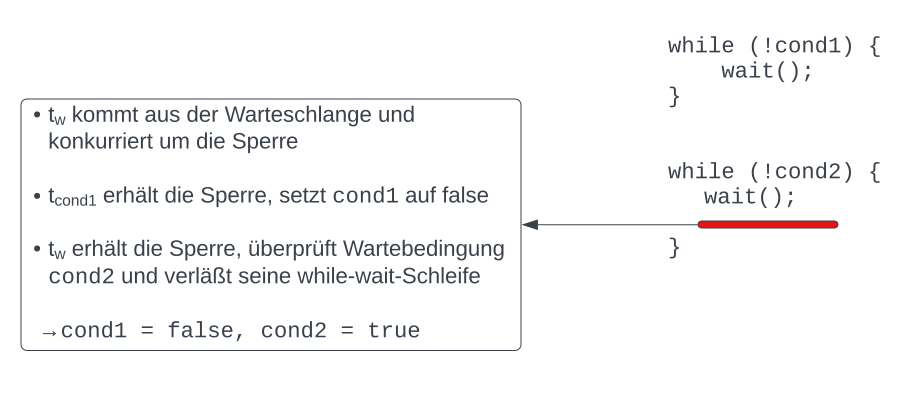
\includegraphics[scale=0.4]{chapters/Anhang/Klausuren/img/cond1cond2}
    \caption{in den rot markierten Bereich konkurriert $t_w$ um die Sperre des Objektes - wenn durch einen anderen Thread, der vor $t_w$ die Sperre erhält, \textit{cond1} auf \textit{false} gesetzt wird, stimmt die Ausgabe nicht mit der erwarteten überein. (Quelle: eigene)}
    \label{fig:cond1cond2}
\end{figure}

\noindent
Die korrekte Wartebedingung sollte lauten:

\begin{minted}[mathescape,
    linenos,
    numbersep=5pt,
    gobble=2,
    fontsize=\small,
    frame=lines,
    framesep=2mm]{java}
    public synchronized void cond1AndCond2() {
        while(!cond1 || !cond2) {
            try {
                wait();
            } catch(InterruptedException e) { }
        }
        System.out.println("cond1 and cond2:" + cond1 + " " + cond2);
    }
\end{minted}\\

Darüber hinaus müßte \code{notifyAll()} nur aufgerufen werden, wenn sowohl \code{cond1} als auch \code{cond2} auf \code{true} gesetzt sind, was leicht in den entsprechenden Methoden überprüft werden kann.
    \chapter{SS19}\label{ch:klausurss19}

\section{Aufgabe 1}

Bei der Aufgabe ist es wichtig, die Anforderungen genau zu beachten.\\
Ob eine Thread die while-wait-Schleife verlassen darf, wird von der Methode \code{tick()} gesteuert - wieviele Ticks ein Thread in der Schleife bleiben soll, wird von dem jeweiligen Thread definiert.\\
Die \code{tick()}-Methode wird von anderen Threads aufgerufen, es kann also durchaus vorkommen, dass mehrmals hintereinander
die \code{notifyAll()}-Methode aufgerufen wird - diese entfernt alle Threads aus der Warteschlange, damit die Threads ihre
Wartebedingungen erneut überprüfen können.\\
da \code{tick()} aber auch gleichzeitig einen Zähler realisieren soll, \textit{muss} es in der Methode auch eine Zählvariable geben, anhand derer die in der while-wait-Schleife enthaltenen Threads feststellen können, wie oft \code{tick()} aufgerufen wurde, um entsprechend aus der Schleife und nachfolgend der Methode herauszukommen.

\begin{figure}
    \centering
    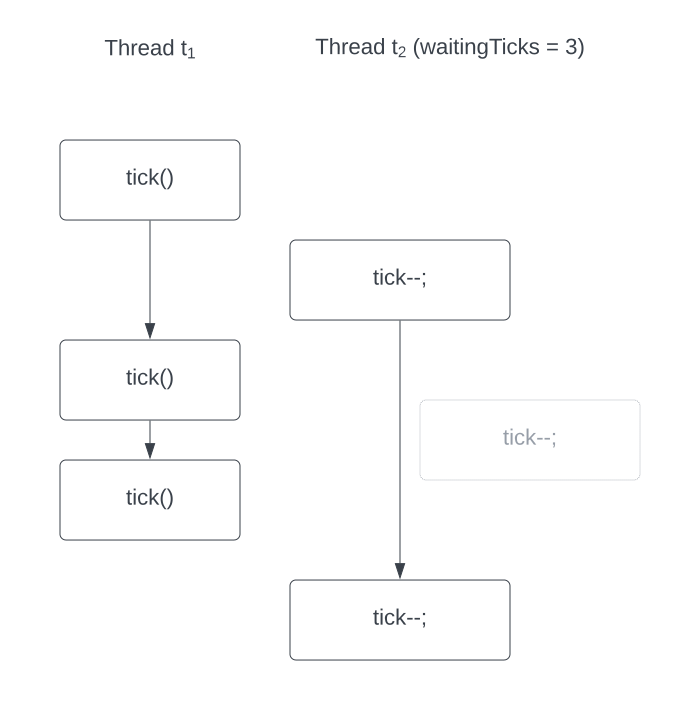
\includegraphics[scale=0.5]{chapters/Anhang/Klausuren/img/tick}
    \caption{Thread $t_1$ ruft 3 mal \texit{tick()} auf. Den Anforderungen nach müsste Thread $t_2$ danach aus der while-wait-Schleife herauskommen, erhält aber nicht die Sperre auf das Objekt von LogicalTime, um seinen eigenen Zähler rechtzeitig zu erniedrigen, bevor $t_1$ erneut \textit{tick()} aufruft. (Quelle: eigene)}
    \label{fig:tick}
\end{figure}

\section{Aufgabe 6}
Auch hier gilt, dass die Aufgabenstellung aufmerksam zu lesen ist.\\
Der Kreis soll erst ausgefüllt werden, wenn die Maustaste gelöst wird.

\begin{minted}[mathescape,
    linenos,
    numbersep=5pt,
    gobble=2,
    frame=lines,
    framesep=2mm]{java}
    private void mousePressed(double x, double y) {
        c = new Circle();
        c.setCenterX(x);
        c.setCenterY(y);
        c.setStroke(Color.RED);
        c.setFill(null); // oder Color.TRANSPARENT
        c.setRadius(RADIUS);
        graphicsPane.getChildren().add(c);
    }

    private void mouseReleased() {
        c.setFill(Color.RED);
        c = null;
    }
\end{minted}

\section{Aufgabe 8}

In der Abbildung \ref{fig:batchmodus} ist links der sequentielle Modus dargestellt, bei dem nach dem Senden einer Nachricht auf die Antwort des Servers gewartet wird, bevor eine neue Nachricht geschickt wird.
Dies wird i.d.R. verwendet, wenn das Senden einer neuen Nachricht abhängig ist von einem Ergebnis, die über die Server-Antwort übermittelt wird, oder wenn mit dem Server interagiert wird (Request abhängig vom Response).\\
Der Batch-Modus auf der rechten Seite der gleichen Abbildung ist schneller, da zwischen dem Senden von Nachrichten nicht auf Antworten gewartet werden müssen. \\
Erst nach dem Senden eine Batches von Nachrichten werden die dem Client zur Verfügung stehenden Antworten ausgelesen.\\

\noindent
In dieser Form des Batch-Modus besteht allerdings die Gefahr, dass es zu Verklemmungen kommt:
\begin{itemize}
    \item Bei dem Client kommen viele Nachrichten an, während er noch sendet.
    \item Die ankommenden Nachrichten für den Client werden gepuffert, bis sie ausgelesen werden (TCP- / OS-seitig).
    \item Läuft der Puffer voll, sorgt die Flusskontrolle (TCP) dafür, dass dem Sender mitgeteilt wird, dass keine Nachrichten mehr empfangen werden können, der Server sendet nicht mehr.
    \item Die zu sendenden Nachrichten des Servers werden in einen Puffer geschrieben.
    \item Der Sende-Puffer des Senders läuft voll.
    \item Bei dem nächsten Sende-Aufruf blockiert der Server, empfangene Nachrichten landen im Empfangspuffer
    \item Der Empfangspuffer des Servers läuft voll, der Client buffert die zu sendenden Nachrichten.
    \item Beide Anwendungen blockieren.
\end{itemize}

\\noindent
Um dieses Problem beim Batch-Modus zu umgehen, werden für das Senden und Empfangen zwei Threads auf Client-Seite erstellt: Ein Thread sendet, ein Thread empfängt. \\
Dadurch kann von dem Client immer wieder sein Empfangspuffer geleert werden, der Server wird beim Senden nicht blockiert.

\begin{figure}
    \centering
    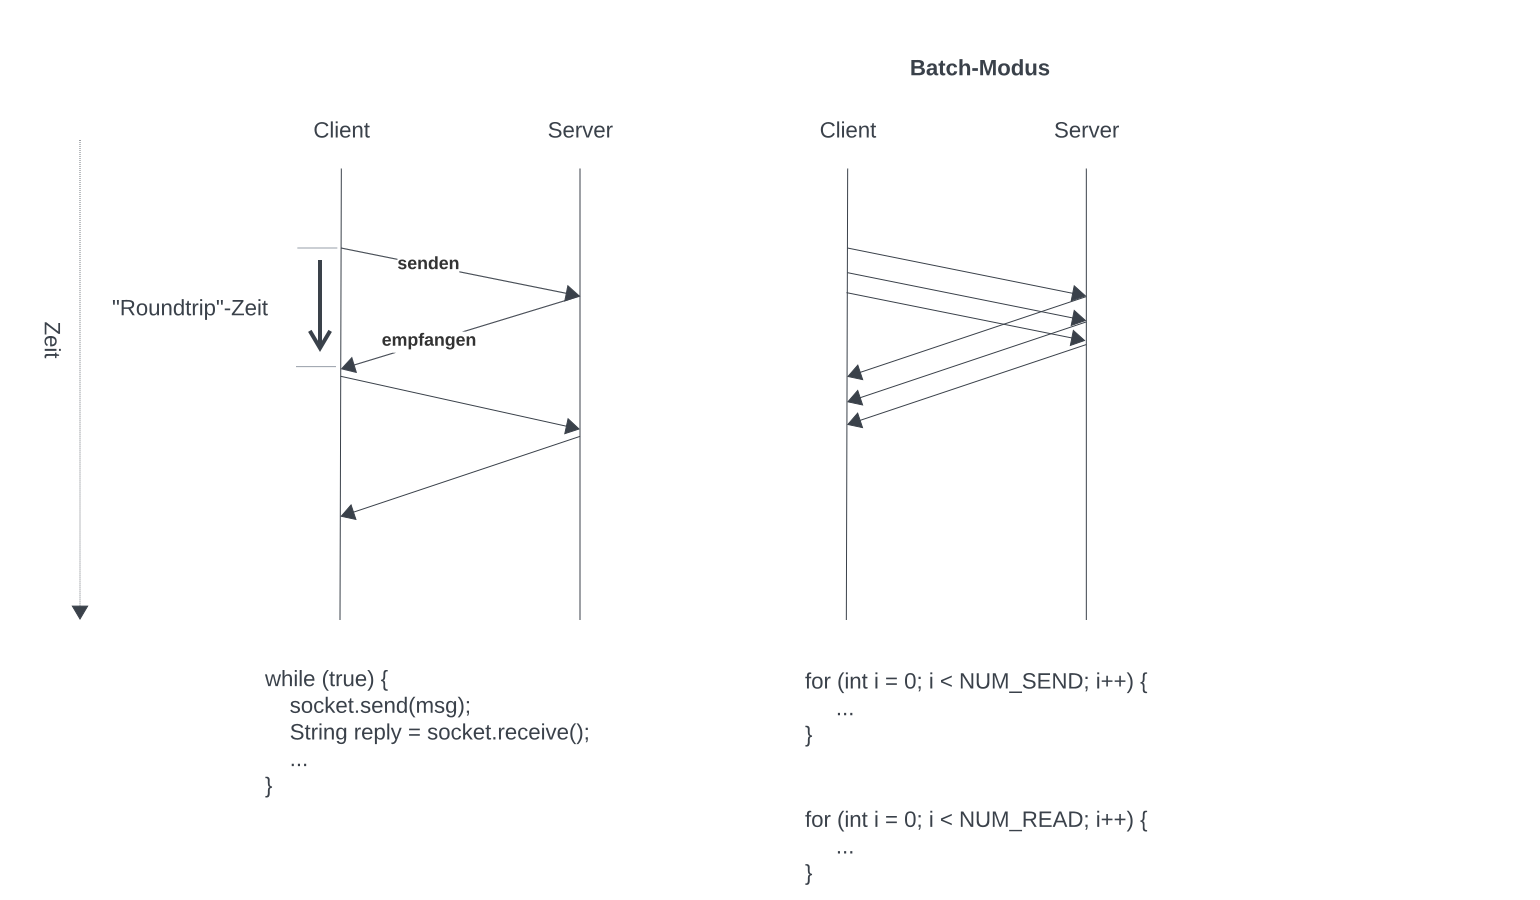
\includegraphics[scale=0.4]{chapters/Anhang/Klausuren/img/batchmodus}
    \caption{Vereinfachte Darstellung sequentieller Kommunikation und Batch-Modus (Quelle: eigene)}
    \label{fig:batchmodus}
\end{figure}
    
\begin{appendices}
    \input{chapters/Anhang/Zusatzaufgaben/index}
    \input{chapters/Anhang/Klausuren/ws13}
    \input{chapters/Anhang/Klausuren/ws15-16}
    \input{chapters/Anhang/Klausuren/ws16-17}
    \input{chapters/Anhang/Klausuren/ss19}
    \input{chapters/Anhang/Präsenzphase/index}

\end{appendices}


\end{appendices}


\end{appendices}

%fopt3
\input{chapters/fopt3/einführung in uml}
\input{chapters/fopt3/einführung in javafx}
%fopt4
\section{MVP}

\textbf{MVP} gehört zu den \textbf{MV*-Architekturmustern}.\\

\noindent
\textbf{Architekturmuster} besitzen wie \textbf{Entwurfsmuster} einen hohen Abstraktionsgrad.\\

\textbf{Entwurfsmuster} werden i.d.R. zur Lösung kleiner Teilbereiche von Software eingesetzt, während \code{Arhictekturmuster} für die gesamte Software oder für größere Teile einer Software eingesetzt werden\footnote{vgl. Skript FOPT4, S. 1}.\\
$\rightarrow$ Enturfsmuster beschreiben eher das Zusammenwirken von Klassen und Schnittstellen.
Architekturmuster sind wie ein Bauplan für ganze Programmteile bzw. Teilbereiche einer Software zu verstehen.

\noindent
zu den Vorteilen von Architekturmustern gehört:

\begin{itemize}
    \item sie helfen, Anwendungen klarer zu strukturieren $\rightarrow$ Leitfaden zur Strukturierung
    \item erleichtert das systematische Testen (durch klare Strukturierung); Änderungen an der Software sind leichter durchführbar
    \item hift, den Code anderer zu verstehen, wenn dieser nach einem bestimmten Muster strukturiert ist
\end{itemize}

\subsection{Prinzip von MVP}

\textbf{MVP} bezeichnet drei Komponenten: \textbf{Model}, \textbf{View}, \textbf{Presenter}.\\

\subsection*{Model}

Das \textbf{Model} ist verantwortlich für
\begin{itemize}
    \item die \textbf{Geschäftslogik}, die den logischen Kern der Anwendung darstellt
    \item die Bereitstellung und das Ändern relevanter Daten für die Anwendung
    \item die Wahrung von Konsistenzbedingungen
    \item die Realisiserung von Persistierung
\end{itemize}

Das Model ist unabhängig von Darstellungs- und Steuerungslogik.

\subsection*{View}

Die \textbf{View} ist die Darstellungskomponente der Software und baut und verändert sie.\\
Mehrere Views können hierbei Teile des Models darstellen.\\
Benutzerinteraktionen werden von der View an den Presenter weitergeleitet.\\

\subsection*{Presenter}
Die \textbf{Präsentationskomponente} ist zuständig für die Ablaufsteuerung, i.d.R. durch vom Bentzer ausgelöste Aktionen, wie bspw. einem Button-click.

\begin{tcolorbox}
Der \textbf{Presenter} hat eine Vermittlerrolle: Er kennt das \textbf{Model} und kann bei Bedarf vermitteln.\\
Im Unterschied zu \textbf{MVC} kennen sich Model und \textbf{View} nicht (s. Abbildung~\ref{fig:mvp}).\\
\end{tcolorbox}

\begin{figure}
    \centering
    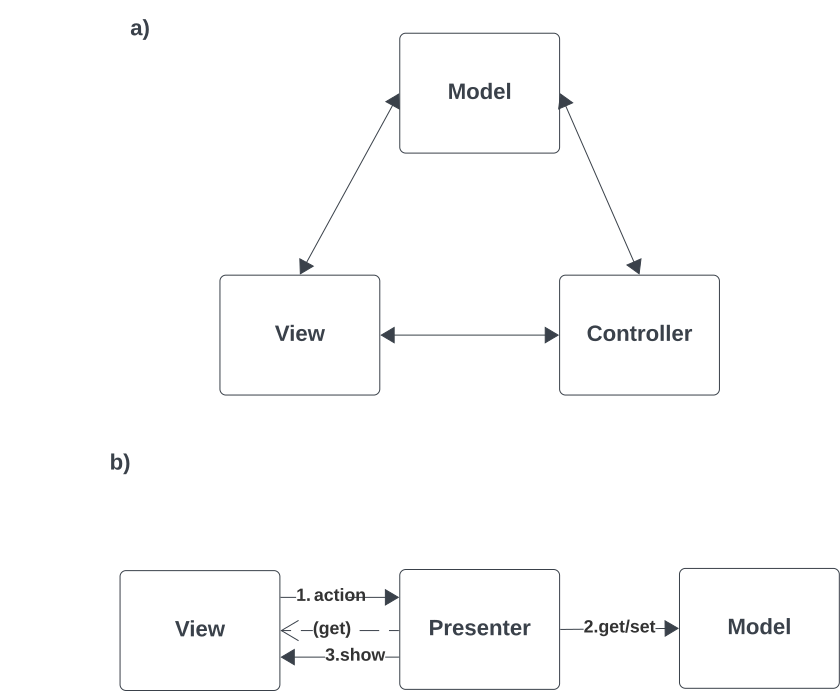
\includegraphics[scale=0.5]{chapters/fopt4/img/mvp}
    \caption{Während bei MVC die Komponenten direkt  Informationen untereinander austauschen können, kennen sich bei MVP Model und View nicht, vermittelt wird über den Presenter. Der Presenter ist auch in der Lage, sich Daten von der View zu beschaffen. (Quelle: in Anlehnung an \cite[223, Bild 4.12]{Oec22})}
    \label{fig:mvp}
\end{figure}


\noindent
Der Presenter kann einen Teil der Validierungslogik enthalten, bspw. zum Erkennen fehlerhafter Eingabedaten.\\

\noindent
Alle Komponenten sind gut testbar:

\begin{itemize}
    \item Das \textbf{Model} hat keien Abhängigkeiten zu \textbf{Presenter} und \textbf{View}.
    \item Der \textbf{Presenter} kann über \textit{Mock-Objekte} (für View & Models) getestet werden
    \item Die \textbf{View} erhält für den Presenter ein Mock-Objekt.
\end{itemize}

\section{Threads und JavaFX}

Stage-Objekte dürfen nciht im \textbf{Main-Thread} erzeugt werden. \\
Das primäre Stage-Objekt wird von der Platform vorgegeben, nachfolgenden Stage-Objekte und UI -Elemente müssen im \textbf{JavaFX Application Thread} erzeugt werden.\\

\noindent
Der \textbf{JavaFX Application Thread} ist auch zuständig für die Ereignisbehandlung - insgesamt gibt es nur einen solchen Thread für die Verwaltung von UI-Elementen und deren Ereignisse. \\

\noindent
Mit der Methode \staticcode{javafx.application.Platform.runLater()}) lassen sich Aktionen am \textbf{JavaFX Application Thread} \textit{anmelden} bzw. in dessen \textit{Warteschlange} einreihen (Parameter vom Typ \code{Runnable}).\\

\subsection*{Regel 1}
Die Durchführung der Ereignisbehandlung sollte in \underline{möglichst kurzer Zeit} abgeschlossen sein, auf \code{sleep()} und \code{wait()} sollte möglichst verzichtet werden.

\subsection*{Regel 2}
Der Zugriff auf grafische Elemente der Oberfläche darf \underline{ausschließlich} durch den \textbf{JavaFX Application Thread} erfolgen.\\
Wenn ein anderer Thread auf die Oberfläche zugreifen möchte, beauftragt der dazu den \textbf{JavaFX Application Thread} durch den Aufruf der Methode \code{Platform.runLater()}.\\
Der Auftrag muss in Form eines \code{Runnable}-Objektes übergeben werden.\\

\noindent
Um Theads, die mit der UI interagieren, mit Beendigung des Hauptprogramms zu beenden, sollte man sie als Daemon-Thread deklarieren\footnote{
``Ein Java-Programm ist zu Ende, wenn alle Threads zu Ende sind - Hintergrund-Threads werden dabei nciht beachtet, nur Vordergrund-Threads (vgl.~\cite[89]{Oec22}).
} (Aufruf der methode \code{setDaemon(true)} auf ein Objekt der Klasse \code{java.lang.Thread}, bevor der Thread gestartet wurde).\\

\noindent
\code{Runnable}s werden in der Reihenfolge durchgeführt, in denen sie mit \code{Platform.runLater()} angemeldet worden sind.

\subsection{Tasks und Services in JavaFX}

JavaFX bietet eine Unterstützung zur Verarbeitung länger andauernder / immer wiederkehrender Aktivitäten im Zusammenhanf mit der UI an, über die generische Schnittstelle \code{Worker} sowie der generischen Klassen \code{Task}, \code{Service}, \code{ScheduledService}.\\

\noindent
\textbf{Task} ermöglicht eine einmalige Ausführung einer länger andauernden Aktivität.\\

\noindent
\texbf{Service} ermöglicht die wiederholte Aktivierung, indem immer wieder Task-Objekte erzeugt werden.\\

\noindent
\textbf{ScheduledService} ermöglicht die periodische ADurchführung von Aktivitäten.\\

\noindent
Properties ermöglichen die Kommunikation zwischen \textbf{Tasks}/\code{Services} und dem \textbf{JavaFX Application Thread}, über sie kommt man sogar ohne \code{Platform.runLater()} aus (der gleichzeitige Gebrauch wird aber nicht ausgeschlossen.)\\

\noindent
Die Methode der Listener, die an diese Properties angemeldet sind, werden immer vom \textbf{JavaFX Application Thread} ausgeführt.\\

\noindent
Beispiele für Properties der Klasse \code{Task}\footnote{
Class Task<V>: \url{https://docs.oracle.com/javase/8/javafx/api/javafx/concurrent/Task.html} - abgerufen 29.01.2024
}:

\begin{itemize}
    \item \code{message}: Meldungen von Threads aus dem \textbf{JavaFX Application Thread; die Threads können über \code{updateMessage()}} den Inhalt ändern
    \item \code{title:} wie \code{message} (analoge Funktion: \code{setTitle()})
    \item \code{value}: ähnlich \code{message} und \code{title} (Methode: \code{updateValue()}); der Typ ist \code{ReadOnlyObjectProperty<V>}, wobei \code{V} der generische Typ der Klasse \code{Task} ist.
    \item \code{workDone} / \code{totalWork}: Indikator zum Fortschritt (Relation geleistete Arbeit zur gesamten Arbeit).
    \code{updateProgress()} ermöglicht die Aktualisierung beider Werte auf einmal
    \item \code{progress}: nur lesender Zugriff, liefert immer $\frac{workDone}{totalWork}$, also den Quotienten
    \item \code{state}: liefert den zustand des Tasks (\code{READY}, \code{RUNNING}, \code{SUCCEEDED}, \code{FAILED}, \code{CANCELLED})
\end{itemize}

Um \code{Task} zu verwenden, leitet man eine eigene Klasse von \code{Task} ab und überschreibt \code{call}; in der Methode lässt sich \code{updateValue} und \code{updateProgress} aufrufen (der Rückgabetyp von \code{call} its der Typparameter der KLasse \code{Task}; für \code{extends Task<Double>} also \code{Doubel}).\\
\code{call} sollte überprüfen, ob \code{cancel} aufgerufen wurde (\code{isCancelled}), um die Bearbeitung abzubrechen (im Gegensatz zum \code{interrupt}-Flag bei Threads ist der Zustand des \clode{cancel}-Flags aber persistent).\\

\noindent
\code{Service}s sind für wiederholte Ausführungen länger andauernde Aktivitäten vorgesehen: Services erzeugen hierfür bei jeder wiederholten Ausführung ein neues \code{Task}-Objekt; ein Service kann mittels \code{start()} direkt gestartet werden, ein \code{Task} implementiert die \code{Runnable}-Schnittstelle und wird einem Thread übergeben, der gestartet werden muss.

\begin{minted}[mathescape,
    linenos,
    numbersep=5pt,
    gobble=2,
    frame=lines,
    framesep=2mm]{java}
    MyTask t = new MyTask();
    Thread t1 = new Thread(t);
    t1.setDaemon(true);
    t1.start();
\end{minted}\\

\noindent
Eine Klasse muss von der abstrakten Klasse \code{Service} abbleiten und darin \code{createTask()} überschreiben, die das entsprechende Task-Objekt zurückliefert.\\

\noindent
Man kann dem Service einen \code{Executor} zuweisen, ansonsten wird ein neuer \code{Daemon}-Thread erzeugt und gestartet.\\

\noindent
Erneutes Starten des Service ist erst möglich, wenn der Service nicht mehr aktiv ist (\code{isRunning}), oder wenn zuvor \code{reset()} aufegrufen wurde.\\
Auch \code{restart()} ermöglicht einen Neustart (ruft intern \code{cancel()} $\rightarrow$ \code{reset()} $\rightarrow$ \code{start()} auf).
%fopt5
\chapter{Verteilte Anwendungen mit Sockets}

Eigenständige \codebf{Client-Server-Anwendungen} können auf 3 verschiedene Arten umgesetzt werden:

\begin{itemize}
    \item Socket-Programmierung (Socket: Schnittstelle für \textbf{UDP} / \textbf{TCP} \footnote{
    UDP: \textit{User Datagram Protocol}; TCP: \textit{Transmission Control Protocol}
    })
    \item \textbf{RMI} \textit{Remote Method Invocation}: Die Methode eines Objektes, das auf einem anderen Rechner liegt, kann von einem anderen entfernten Rechner aufgerufen werden; RMI basiert auf Sockets und stellt somit eine höhere Schnittstelle mit einem höheren Abstraktionsniveau dar
    \item \textbf{indirekte Kommunikation}: Nachrichten werden durch einen Vermittler von einem Sender zu einem Empfänger weitergeleitet
\end{itemize}


\subsection{Schichtenmodell}

\subsection*{Schicht 1 - (Physical Layer)}

Diese Schicht ist zuständig für die Übertragung von Datenblöcken zwischen zwei Rechnern, die direkt miteinander verbunden sind (genauso wie \textbf{Schicht 2}).\\
Sie ist zuständig für die Übertragung einzelner Bits und wird deshalb auch \textbx{Bitübertragungsschicht} genannt.

\subsection*{Schicht 2 - DataLink Layer}

Wie Schicht 1 ist auch diese Schicht zuständig für die Übertragung von Datenblöcken zwischen zwei direkt miteinander verbundenen Rechnern.\\

Die Schicht hat die Aufgabe, einzelne Bits zu einem Datenblock in einem bestimmten Format zusammenzufassen.\\
$\rightarrow$ bestimmte Informationen wie z.B. Adressen haben eine bestimmte Struktur und Bitlänge und stehen an bestimmten Stellen in einem Datenblock.\\

\noindent
Bei lokalen Netzen wie {bspw.} Ethernet hat die \textbf{Leitungsschicht} durch das gemeinsame Medium noch weitere Funktionen: Sie garantiert, dass immer nur höchstens eine Station sendet, außerdem werden durch sie die angeschlossenen Rechner korrekt adressiert\footnote{
``Bei einer Punkt-zu-Punkt-Leitung kann eine empfangene Station davon ausgehen, dass die ankommenden Daten für sie bestimmt sind, bei einem gemeinsamen Medium dagegen nicht.``~\cite[257]{Oec22}
}

\begin{tcolorbox}
    Schicht 1 und 2 werden über Hardware ({bspw.} Ethernet-Adapter) und entsprechende Treiber im Betriebssystem realisiert.
\end{tcolorbox}

\noindent
Die beiden Funktionen (eine Station sendet, korrekte Adressierung) werden als \textbf{Medium Access Control} (\textit{MAC}) bezeichnet und bilden eine Teilschicht innerhalb der Leitungsschicht (\textit{DataLink Layer}).\\
Die entsprechenden Adressen heissen deshalb \textit{MAC-Adresssen}.

\subsection*{Schicht 3}
Schicht 3 ist die \textbf{Vermittlungsschicht} (\textbf{Network Layer}), hier befindet sich das \textbf{IP-Protokoll}, über das Rechner verbunden werden, die an verschiedene Netze mit unterschiedlichen Netztechnologien angeschlossen sind.\\

\noindent
Jeder Netzanschluss enthält eine eindeutige \textbf{IP-Adresse}.\\
Die Schicht sorgt für eine einheitliche, strukturierte und weltweit eindeutige Adressierung (vgl.~\cite[258]{Oec22}).\\

\noindent
Über das IP-Protokoll werden Datenpakete über verschiedene Netze weitergeleitet, bis sie beim Zielrechner ankommen.\\

\noindent
Es kann durchaus vorkommen, dass Datenpakete verlorengehen, oder verzögert und/oder in unterschiedlicher Reihenfolge beim Empfänger eintreffen.


\begin{tcolorbox}
    Schicht 3 und 4 sind i.d.R. Teil des Betriebssystemkerns.
\end{tcolorbox}

\subsection*{Schicht 4}
Schicht 4 ergänzt die Adressierung in Schicht 3 um \textit{Konktaktpunkte} durch \textbf{Portnummern}, und wird \textbf{Transportschicht} (\textbf{Transport Layer}) genannt.\\

\noindent
Zwei verbreitete Transportprotokolle sind \textbf{UDP} und \textbf{TCP};

\begin{itemize}
    \item \textbf{UDP} (\textit{User Datagram Protocol}) hat dieselbe Eigenschaften wie das IP-Protokoll und erweitert es um die Adressierung mit Portnummern.\\
    Es ist genauso   \textit{verbindungslos} und \textit{unzuverlässig}\footnote{
    es sind Verluste und Reihenfolgevertauschungen möglich.
    } wie das IP-Protokoll.
    \item \textbf{TCP} (\textit{Transmission Control Protocol}) behebt die Nachteile des IP-Protokolls: Die Empfänger müssen den Nachrichtenerhalt bestätigen\footnote{ \textbf{ACK},
    was wiederum von Sender-Seite überwacht wird; s.a. ``Transmission Control Protocol``: \url{https://en.wikipedia.org/wiki/Transmission_Control_Protocol} - abgerufen 30.01.2024
    }, ansonsten wird die Nachricht nochmals gesendet.
\end{itemize}


\subsection*{Schicht 5}
Schicht 5 ist die \textbf{Anwendungsschicht}\footnote{
    Im Buch werden 5 Schichten aufgeführt, das \textbf{OSI-Modell} hat in der \textit{Anwendungsorientierten Schicht} noch zwei zusätzliche Schichten, die \textbf{Session-Layer} und die \textbf{Presentation-Layer} (\url{https://en.wikipedia.org/wiki/OSI_model} - abgerufen 3.2.2024)
} (\textbf{Application Layer}), in ihr wird die Kommunikation der Anwendung abgewickelt (bspw. \textit{www}, \textit{email}, \textit{Videokonferenzen}).


\begin{tcolorbox}
    Schicht 5 wird über Anwendungsprozesse realisiert.
\end{tcolorbox}


\begin{figure}
    \centering
    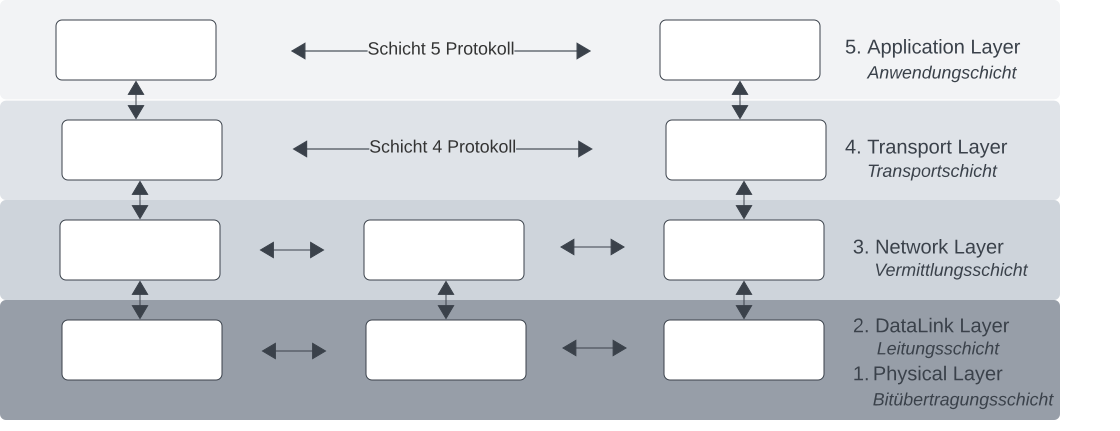
\includegraphics[width=16cm]{chapters/fopt5/img/layers}
    \caption{Skizze des Schichtenmodels. (Quelle: in Anlehnung an \cite[257, Bild 5.2]{Oec22})}
    \label{fig:layers}
\end{figure}


\subsection{IP-Adressen und DNS-Namen}

Ein Rechner kann mehrere Netzanschlüsse haben.\\

\noindent
Jeder dieser Netzanschlüsse ist eine weltweit eindeutige IP-Adresse zugeordnet.\\

\noindent
IP-Adressen können auch durch (Rechner-)Namen aufgelöst werden durch das \textbf{Domain Name System} (\textit{DNS}).\\

\noindent
Ein DNS-Name kann auch mehrere Aliase besitzen; dadurch, dass ein Rechner mehrere IP-Adressen haben kann (bspw. durch mehrere Netzanschlüsse) besteht so zwischen Rechnernamen und IP-Adressen eine $m:n$-Beziehung.


\subsection{Das Transportportprotokoll UDP}

Transportprotokolle existieren, damit mehrere Anwendungen, die über das Internet kommunizieren, gleichzeitig laufen und Daten untereinander austauschen können.\\

\noindent
Bei der Übertragung von Daten besitzt IP die Eigenschaften, dass Daten in unterschiedlicher Reihenfolge eintreffen können, was aus Anwendersicht problematisch ist; auf Anwendungsschicht könnte man hier Gegenmaßnahmen treffen, aber das würde bedeuten, die Gegenmaßnahmen in jeder Anwendung implementieren zu müssen - deshalb werden diese Problematiken in der \textbf{Transportschicht} über \textbf{Transportprotokolle} gelöst.\\

\noindent
\textbf{UDP} (\textbf{User Datagram Protocol}) ermöglicht die Kommunikation verschiedener Dienste gleichzeitig (spezifische Anwendung wird über Portnummer adressiert).\\

\noindent
Ein \textbf{Datagramm}\footnote{
Kunstwort abgeleitet aus\textit{Telegramm} (vgl.~\cite[260]{Oec22})
} bezeichnet eine Dateneinheit, die in ein IP-Paket gepackt und über das Netz verschickt wird.\\

\begin{tcolorbox}
\textbf{UDP} ist Nachrichtenorientiert.
\end{tcolorbox}

\noindent
Ein \textbf{UDP-Datagram} enthält neben der Zielportnummer auch die Quellportnummer, damit der Empfänger dem Sender antworten kann.

\noindent
UDP ist wie IP \textbf{verbindungslos} - es können \textit{Datagrammverluste} oder \textit{Reihenfolgevertauschungen} von Datagrammen vorkommen.\\

\noindent
UDP ist \textbf{datagrammorientiert}: Eine an das UDP-Protokoll übergebene Menge an Daten wird in ein Datagramm gepackt und über IP verschickt\\
$\rightarrow$ die Daten kommen als Einheit beim Empfänger an (entspricht dem Verhalten einer \textbf{Message Queue})


\subsection{Das Transportprotokoll TCP}

\textbf{TCP} ist ein Protokoll für genau zwei Partner, weshalb es nicht mit \textbf{Multicast} genutzt werden kann.\\

\noindent
\textbf{TCP} ist verbindungsorientiert, wobei der Verbindungsauf- und -abbau einen gewissen Aufwand erfordert\footnote{
    Wenn Datenverluste nicht hinnehmbar sind und wegen höherem Aufwand für die Verbindung trotzdem UDP verwendet wird, erweitert man die Anwendung entsprechend um Gegenmaßnahmen für den Datenverlust (vlg. \cite[261]{Oec22}).
}.

\noindent
\textbf{TCP} ist ein zuverlässiges Protokoll, es können keine Daten vertauscht oder verloren gehen, außerdem gibt es eine \textbf{Flusskontrolle} (zum Verhindern einer Überflutung des Empfängers mit Datenpaketen)\footnote{Empfangsbestätigung abwarten} und eine \textbf{Überlastkontrolle} (um eine Überlastung des Netzes zu verhindern)\footnote{informal: falls ein ACK ausbleibt, könnte der Sender versucht sein, ständig neue Pakete hinterherzuschicken, was zu einem Stau führen könnte. Siehe hierzu auch ``Modul 6: TCP-Überlastkontrolle``: \url{https://leischner.inf.h-brs.de/lehre/ikomm/ikomm06-ueberlastkontrolle.pdf} - abgerufen 30.01.2024}.\\

\noindent
\textbf{TCP} ist \textbf{datenstromorientiert} - der Empfänger erkennt an dem Datenstrom nicht, in welchen Portionen die Daten vom Sender geschickt wurden (entspricht dem Verhalten von \textbf{Pipes} (s. a. Abschnitt~\ref{sec:messagequeues})).


\setlength{\tabcolsep}{0.8em}
{\renewcommand{\arraystretch}{1.7}%
\begin{table}
[htbp]
    \centering

    \begin{tabular}{|l|l|}
        \toprule
        \hline
        \textbf{UDP} & \textbf{TCP}  \\
        \midrule
        \hline
        verbindungslos & verbindungsorientiert \\
        \hline
        unzuverlässig  & zuverlässig mit Fluss- und Überlastkontrolle \\
        \hline
        datagrammorientiert & datenstromorientiert \\
        \hline
        \bottomrule
    \end{tabular}

    \caption{Vergleich zwischen UDP und TCP. (Quelle: in Anlehnung an \cite[261, Tabelle 5.1]{Oec22})}

\end{table}








\section{Socket-Schnittstelle}

Die \textbf{Socket-Schnittstelle} ermöglicht die Kommunikation von verteilten Client-Server-Anwendungen untereinander.\\

\begin{tcolorbox}
Die Socket-Schnittstelle stellt eine Schnittstelle zwischen \textbf{Schicht 4} (Transportschicht) und \textbf{Schicht 5} (Anwendungsschicht) dar.
\end{tcolorbox}

\subsection{Socket-Schnittstelle zu UDP}

Eine Schnittstelle zu \textbf{UDP} ist relativ einfach zu realisieren, da hier keine Operationen für den Verbindungsauf- und -abbau nötig sind $\rightarrow$ es sind nur Operationen für das Senden und Empfangen notwendig.\\

\noindent
Bei der Erzeugung eines \textbf{Sockets} kann eine Portnummer angegeben werden, für gesendete Nachrichten ist das dann die \textbf{Quellportnummer} der Nachricht.\\
Der Socket empfängt nur Nachrichten, die an diesen Port adressiert wurden.\\

\noindent
Bei \textbf{Client/Server-Anwendungen} geht die Initiative vom Client aus, der eine Anfrage an einen Server schickt.\\
Der Server antwortet an die in der Nachricht enthaltenen IP-Adresse und Quellportnummer.

\begin{tcolorbox}
I.d.R verwendet ein Client eine beliebige freie Portnummer.\\

\noindent
Dienste laufen auf Servern auf wohlbekannten Portnummern, bspw. ``https`` auf Port $443$\footnote{
s. a. ``Hypertext Transfer Protocol Secure``: \url{https://de.wikipedia.org/wiki/Hypertext_Transfer_Protocol_Secure} - abgerufen 30.01.2024
}.\\
Ein Server, der unter einer bestimmten Portnummer laufen soll, kann nur gestartet werden, wenn die Postnummer nicht schon belegt ist.
\end{tcolorbox}\\

Beispiel für eine Programmstruktur für eine Kommunikation zwischen UDP-Client und -Server:
\begin{minted}[mathescape,
    linenos,
    numbersep=5pt,
    gobble=2,
    frame=lines,
    framesep=2mm]{java}
    // UDP Client
    c = ErzeugeUDPSocket();
    while (beliebig) {
        sende Nachricht über Socket c an ServerAdresse/Portnummer;
        warte auf Nachricht an Socket c;
        tue etwas mit der Nachricht;
    }

    // UDP Server
    s = ErzeugeUDPSocketAnPort(port);
    while (beliebig) {
        warte auf Nachricht von Client an Socket s;
        analysiere die Nachricht;
        führe Aktion aus;
        schicke über s Antwort an die Adresse/Portnummer der Nachricht;
    }
\end{minted}\\


\begin{tcolorbox}
    Die Portnummern für \textbf{TCP} und \textbf{UDP} existieren unabhängig voneinander: Ist ein Port $n$ für TCP reserviert, kann die gleiche Portnummer trotzdem für UDP verwendet werden.
\end{tcolorbox}

\subsection{Socket-Schnittstelle zu TCP}

Die Besonderheit bei TCP ist, dass der Server auf einen Port auf eine Anfrage (über einen Socket) wartet, und dann mit dem Client die Kommunikation über einen neuen Socket realisiert (s. Abbildung~\ref{fig:tcpsockets}).\\

\begin{figure}
    \centering
    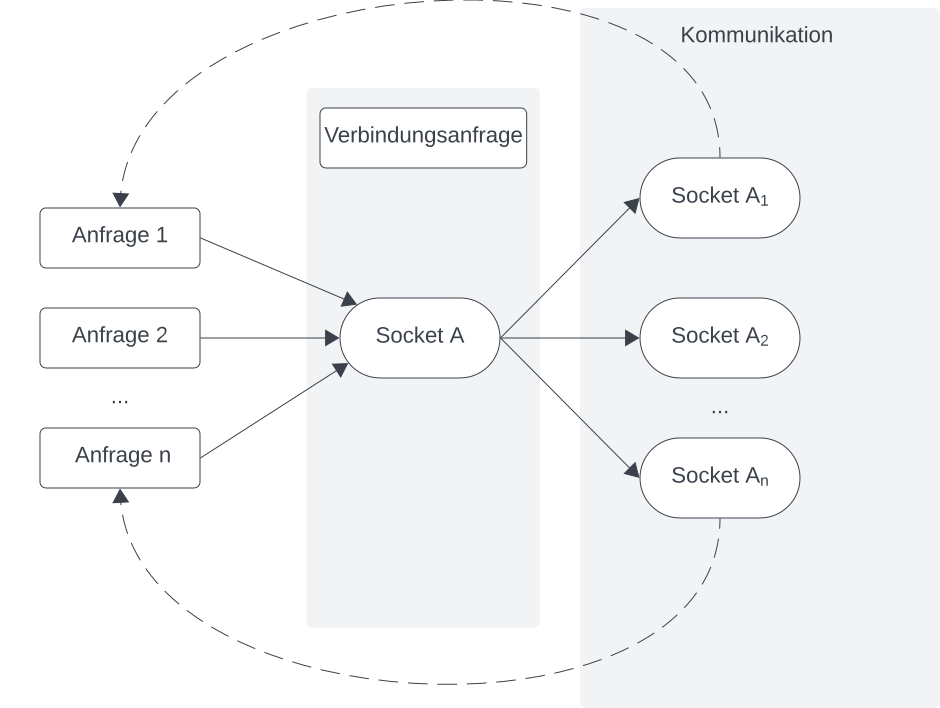
\includegraphics[scale=0.5]{chapters/fopt5/img/sockets/tcpsockets}
    \caption{Von einem TCP-Socket angenommene Verbingungsanfragen führen zu neuen Sockets, die letztendlich für die Kommunikation mit den Clients verantwortlich sind. (Quelle: eigene)}
    \label{fig:tcpsockets}
\end{figure}



\noindent
$\rightarrow$ für einen Port kann es somit mehrere Sockets geben.\\

Beispiel für eine Programmstruktur für eine Kommunikation zwischen UDP-Client und -Server:
\begin{minted}[mathescape,
    linenos,
    numbersep=5pt,
    gobble=2,
    frame=lines,
    framesep=2mm]{java}
    // TCP Client
    c = ErzeugeTCPSocket();
    baue über c eine Verbindung zu ServerAdresse/Portnummer auf;
    /* c ist blockiert, bis Timeout abgelaufen oder Anfrage angenommen */
    while (beliebig) {
        sende Nachricht über Socket c;
        warte auf Nachricht an Socket c;
        tue etwas mit der Nachricht;
    }
    schliesse die Verbindung über c;

    // TCP Server
    s = ErzeugeTCPSocketAnPort(port);
    while (beliebig) {
        warte auf Verbindungsanfrage an s und erstelle
        neuen Socket q;

        while (Verbindung besteht) {
            warte auf Nachricht von Client an Socket q
            wenn nachricht da ist {
                analysiere die Nachricht;
                führe Aktion aus;
                schicke über q Antwort an die Adresse/Portnummer
                der Nachricht;
            } ansonsten nach timeout oder verbindungsabbruch {
                schliesse Verbindung über q;
                verlasse die innere schleife und warte auf
                neue verbindung;
            }

        }
    }
\end{minted}\\

\noindent
Es gibt bei \textbf{TCP} höchstens eine Verbindung von einem Port auf einem Rechner zu einem anderen Port auf einen anderen Rechner, aber es können mehrere Verbindungen von einem Port zu unterschiedlichen Ports des Zielrechners existieren, bzw. es kann ein Rechner mehrere Verbindungen zu einem bestimmten Port auf einem unterschiedlichen Zielrechner erstellen (s. Abbildung~\ref{fig:tcpconnections}).


\begin{figure}
    \centering
    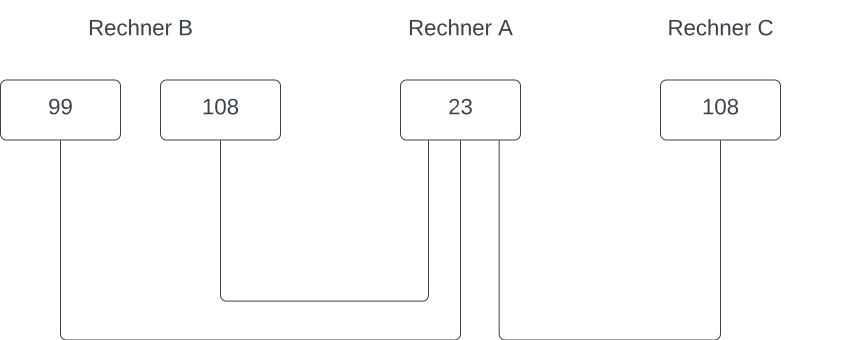
\includegraphics[scale=0.5]{chapters/fopt5/img/sockets/tcpconnections}
    \caption{Rechner $A$ bedient zweimal dieselbe Portnummer $108$ auf zwei unterschiedlichen Rechnern $B$ und $C$, von Port $23$ aus. Gleichzeitig wird Port $99$ von Rechner $B$ von Rechner $A$ bedient. (Quelle: in Anlehnung an \cite[265, Bild 5.3]{Oec22})}
    \label{fig:tcpconnections}
\end{figure}


\subsection{Socket-Schnittstelle für Java}

Die Java-Klassenbibliothek enthält u.a. im Package \code{java.net} Implementierung zur Realisierung von Socket-Kommunikation.\\

\noindent
\code{InetAddress} ist eine Klasse zur Handhabung von von Rechnernamen / IP-Adressen.\\

\noindent
\code{DatagramPacket} und \code{DatagramSocket} werden zur \textbf{UDP}-Kommunikation verwendet.\\

\noindent
\code{Socket} und \code{ServerSocket} werden zur \textbf{TCP}-Kommunikation benötigt.



\section{Verteilte Anwendungen mit RMI}

Wenn man eine verteilte Java-Anwendung entwickeln soll, bei der Kommunikationsprotokoll und Client- und Server-Seite in Java implementiert werden, ist \textbf{RMI} die bessere Alternative gegenüber  \textbf{Sockets} (vgl.~\cite[311]{Oec22}).\\


\begin{tcolorbox}
    \textbf{Remote Method Invocation} ermöglicht das Aufrufen von Methoden auf Objekten, die sich auf demselben oder einem anderem Rechner als der Aufrufer befinden, und damit als unterschiedliche Prozesse in unterschiedlichen Adressräumen ausgeführt werden.
\end{tcolorbox}

\noindent
\textbf{Remote Method Invocation} (RMI) stellt eine Schnittstelle zur Nutzung der Internetprotokolle \textbf{TCP} und \textbf{UDP} bereit.\\
Für RMI ist ein Protokoll auf Schicht 5 definiert, das Daten, deren Reihenfolge und Codierung bei Methodenaufrufen und Methodenrückkehr festlegt (vgl.\cite[402]{Oec22}).

\noindent
\textbf{RMI} verfolgt den Ansatz, OOP auch für die Kommunikation zwischen verteilten Anwendungen zu realisieren, wobei der Aspekt der Verteilung für die Entwickler weitestgehend transparent bleibt

\begin{figure}
    \centering
    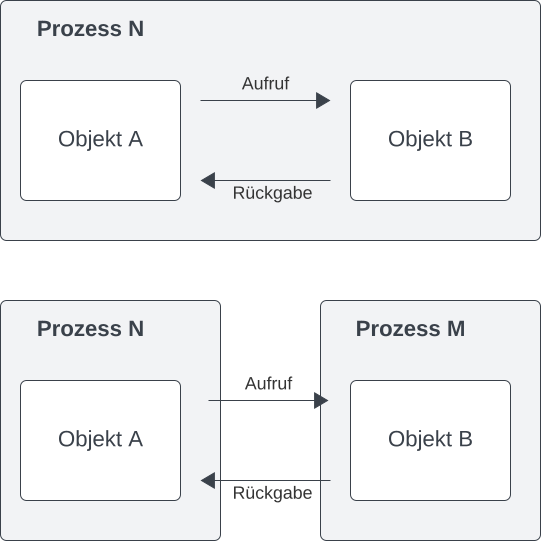
\includegraphics[scale=0.5]{chapters/fopt5/img/rmi/processcall}
    \caption{Zwei unterschiedliche Objekte in unterschiedlichen Aufrufsituationen. Im oberen Beispiel befinden sich die Objekte im selben Adressraum, im unteren Beispiel in unterschiedlichen Adressräumen - diese Situation kommt bei der Nutzung von RMI vor (Quelle: in Anlehnung an \cite[311 f., Abbildung 6.1 und 6.2]{Oec22})}
    \label{fig:processcall}
\end{figure}

\noindent
Die \textbf{Vereilungstransparenz} wird bei \textbf{RMI} über \textbf{Stubs} und \textbf{Skeletons} realisiert.\\

\noindent
Ein \textbf{Stub} implementiert dieselbe Schnittstelle wie das Objekt, das über Fern-Methodenaufrufe \ul{auf dem Server gesteuert werden soll}.

\noindent
Ein \textbf{Skeleton} nimmt die Nachrichten, die vom \textbf{Stub} über die aufgebaute \textbf{TCP}-Verbindung gesendet werden, entgegen und ruft die Methoden auf dem entsprechenden Server-Objekt auf.\\
$\rightarrow$ Ein \textbf{Skeleton} besitzt die Struktur eines \textbf{TCP}-Servers.

\begin{figure}
    \centering
    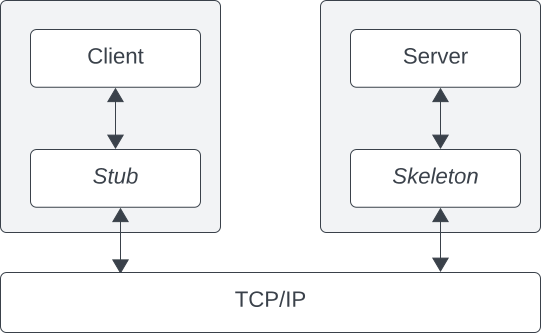
\includegraphics[scale=0.4]{chapters/fopt5/img/rmi/stubskeleton}
    \caption{Prinzip der Kommunikation zwischen RMI-Client und -Server. (Quelle: in Anlehnung an \cite[312, Bild 6.3]{Oec22})}
    \label{fig:stubskeleton}
\end{figure}

\begin{tcolorbox}
    Struktur einer RMI Anwendung\footnote{vgl. im folgenden \cite[162 ff.]{HM05}; \textbf{Stubs} und \textbf{Skeletons} werden automatisch generiert.}:\\


    \noindent
    \textbf{RMI-Client}\\
    Ein \textbf{RMI-Client} fragt bei einem \textbf{RMI-Namensdienst} eine Referenz auf ein entferntes Objekt an, das danach wie ein lokales Objekt behandelt wird.
    Die notwendige Netzwerk-Kommunikation für diese Methodenaufrufe ist transparent und wird automatische abgewickelt.\\


    \noindent
    \textbf{Stub-Objekt}
    \begin{itemize}
        \item Ein \textbf{Stub-Objekt} ist ein \textbf{Stellvertreter} für das entfernte Objekt bei dem RMI-Server.
        Methodenaufrufe des \textbf{RMI-Clients} auf ein entferntes Objekt werden an das Stub-Objekt \textit{delegiert}.
        \item Verantwortlichkeiten: Weiterleitung von Methodenaufrufe an das entfernte Objekt. \textit{Marshalling} von Übergabeparametern und \textit{unmarshalling} von Rückgabewerten\footnote{
          Serialisierung: Umwandeln einer Objektstruktur in ein speicherbares Format. Marshalling bezieht sich auf das Bewegen von Objekten zwischen Threads und Programmen, wofür auch eine Form von Serialisierung notwendig ist. S. a. ``Marshalling (computer science): \url{https://en.wikipedia.org/wiki/Marshalling_(computer_science)} - abgerufen 1.2.2024
        }.
        \item Der Stub wird für jede Anwendung automatisch erzeugt (vgl.\cite[313]{Oec22}).
    \end{itemize}\\

    \noindent
    \textbf{Skeleton-Objekt}\\
   Ein \textbf{Skeleton-Objekt} ist ein \textit{server-seitiger} \textbf{Stellvertreter} für das aufrufende Objekt bei dem RMI-Server, uns unterstützt ebenfalls  \textit{Marshalling} von Übergabeparametern und \textit{unmarshalling} von Rückgabewerten. Das Sekeleton-Objekt ist als Programmteil in der RMI-Implementierung dabei und kann für alle RMI-Anwendungen verwendet werden (vgl.\cite[313]{Oec22}).\\

    \noindent
    \textbf{RMI-Registry}\\
    Die \textbf{RMI-Registry} realisiert einen \textit{Namensdienst}: Eine Abbildung von Namen auf entfernte Objekte.\footnote{
        s.a: ``Kapitel 6: Verteilte Objekte durch RMI``: \url{https://www.informatik.uni-marburg.de/~mathes/download/k6.pdf}, ``Distributed object communication``: \url{https://en.wikipedia.org/wiki/Distributed_object_communication} - beides abgerufen 1.2.2024
    }. \\
    Der \textbf{RMI-Client} fordert hier die Referenzen auf entfernte Objekte an.\\

    \noindent
    \textbf{RMI-Server}\\
    Ein \textbf{RMI-Server} instanziiert ein entferntes Objekt und registriert es unter einem Namen bei der \textbf{RMI-Registry}, und wartet \textit{passiv} auf den Aufruf einer Methode durch den \textbf{RMI-Client}.

\end{tcolorbox}

\begin{figure}
    \centering
    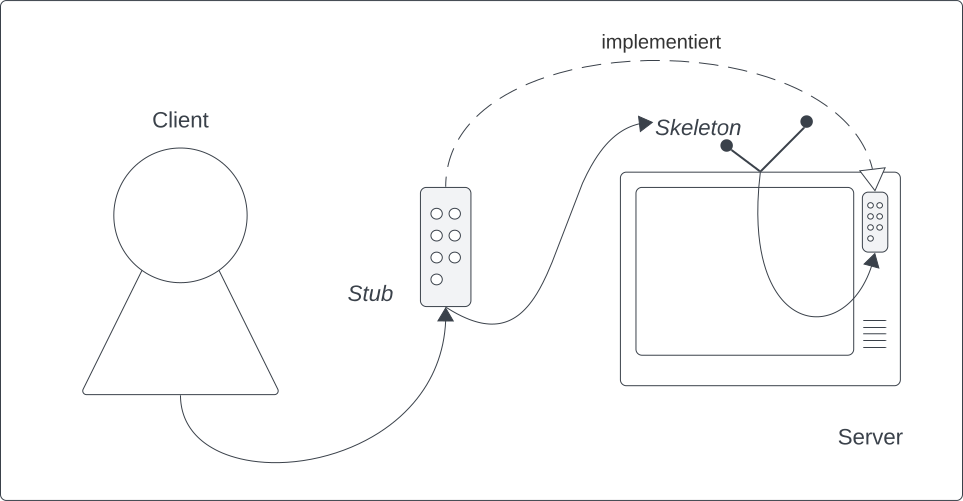
\includegraphics[scale=0.35]{chapters/fopt5/img/rmi/tv}
    \caption{Eine Illustration der im Lehrbuch verwendeten RMI-Metapher. Ein Client will ein entferntes Objekt (TV) bedienen. Hierzu verwendet er Methodenaufrufe, die vom Stub (Fernbedienung) weitergeleitet werden. Die Methoden werden vom Skeleton (Fensehantennen) an das Objekt auf dem Server weitergeleitet. Dieses Objekt sind in dem Beispiel die Knöpfe an dem Fernseher, die die gleichen Bedienfunktionen (``Schnittstelle``) wie die Fernbedienung haben. (Quelle: eigene)}
    \label{fig:tv}
\end{figure}

\noindent
Die \textbf{Transparenz} kommt für den Entwickler dadurch zustande, dass er nur Client und Server, nicht aber Stub und Skeleton programmieren muss.\\
$\rightarrow$ \textbf{Stub} wird automatisch erzeugt, das \texbf{Skeleton}-Objekt ist ein Programmteil, der in der \textbf{RMI}-Implementierung dabei ist und für alle Anwendungen verwendet werden kann.\\

\noindent
Die Entwicklung einer \textbf{RMI}-Anwendung erfolgt i.d.R. in folgenden Schritten\footnote{
s.a. ``An Overview of RMI Applications``: \url{https://docs.oracle.com/javase/tutorial/rmi/overview.html} - abgerufen 1.2.2024
}:

\begin{enumerate}
    \item\label{itm:intdef} \textbf{Schnittstelle definieren}\\
    \noindent
    Die Schnittstelle zwischen Client & Server in Abhängigkeit von der Anwendung, die realisiert werden soll.\\
    \noindent
    Die Schnittstelle führt alle Methoden auf, die über \textbf{RMI} aufgerufen werden sollen.\\
    \noindent
    Die Schnittstelle muss aus \code{java.rmi.Remote} abgeleitet werden.\\
    \noindent
    Alle Methoden der Schnittstelle müssen mit \code{throws RemoteException} gekennzeichnet werden\footnote{
    s.a. ``2.4.1 The java.rmi.Remote Interface``: \url{https://docs.oracle.com/en/java/javase/21/docs/specs/rmi/objmodel.html#the-java.rmi.remote-interface} - abgerufen 1.2.2024
    }.

    \item \textbf{Schnittstelle implementieren}\\
    \noindent
    Es wird eine Klasse geschrieben, die die im ersten Schritt definierte Schnittstelle implementiert.\\
    \noindent
    Einem Objekt davon muss \ul{von aussen über RMI} nutzbar sein - es muss exportiert werden können.
    Dazu kann die implementierende Klasse von \code{UnicastRemoteObject} abgeleitet werden.\\
    Es muss ein expliziter Konstruktor existieren, der mit \code{throws RemoteException} gekennzeichnet wird. \\
    $\rightarrow$ Es muss mindestens ein expliziter Standard-Konstruktor existieren, der diese Bedingung erfüllt\footnote{
    ansonsten wird vom Compiler ein Standard-Konstruktor zur Verfügung gestellt.
    Da dieser aber keine checked Exception in Form einer \textit{RemoteException} wirft, kommt es zu einem Compilerfehler.
    }

    \item \textbf{Server programmieren}\\
    \noindent
    Man erzeugt eines oder mehrere Objekte der in Schritt 2 implementierten Klasse und meldet diese unter einem beliebigen Namen bei der \textbf{RMI-Registry} an.

    \item \textbf{Client programmieren}\\
    \noindent
    Über die \textbf{RMI-Registry} (Serveradresse und Port müssen dem Client bekannt sein) beschafft sich der Client die in Schritt 3 registrieren Objekte, die als \textbf{Stub} an ihn weitergeleitet werden.\\
    \noindent
    Der Stub kann unter Berücksichtigung der in Schritt 1 definierten Schnittstelle so verwendet werden, als wäre es ein lokales Objekt\footnote{
    ``lokal`` im Sinne von gleicher Prozess / gleicher Adressraum.
    }.\\
    \noindent
    Die Methodenaufrufe werden dann letztendlich auf dem durch das in Schritt 2 definierte \textbf{RMI-Objekt} auf dem Server ausgeführt (Client $\rightarrow$ Stub $\rightarrow$ Skeleton $\rightarrow$ Server).

    \item \textbf{Anwendung übersetzen und ausführen}\\
    \noindent
    Alle Dateien werden kompiliert.
    Vor dem Starten des Programms ist darauf zu achten, dass auf dem Server die \textbf{RMI-Registry} gestartet wird - was aber auch aus dem Programm heraus geschehen kann.
\end{enumerate}

\section{Einführendes RMI-Beispiel}

Auch bei RMI-Implementierungen bei denen mehrere Clients gleichzeitig auf eine Objektinstanz zugreifen, ist (ggfl. nach Anwendung) \code{synchronized} nötig, um ein Objekt für den gleichzeitigen Zugriff zu sperren.\\

\noindent
Sobald über \staticcode{java.rmi.Naming.rebind()} bzw. \staticcode{bind()}\footnote{
textit{bind()} wirft eine \textit{AlreadyBoundException}, falls in der RMI-Registry bereits ein Eintrag mit dem Namen existiert, \textit{rebind()} hingegen ersetzt einen ggf. breits existierenden Eintrag mit gleichem Namen.
} der Server gestartet wurde, wird ein Thread gestartet, der den Skeleton repräsentiert, auf eingehende TCP-Verbindungen wartet.\\

\noindent
der Client frag vom Server über

\begin{minted}[mathescape,
    linenos,
    numbersep=5pt,
    gobble=2,
    frame=lines,
    framesep=2mm]{java}
    java.rmi.Naming.lookup("rmi://serveradresse/bindingname");
\end{minted}\\

das Objekt ab, auf das er zugreifen möchte, und bekommt dann ein Objekt vom Typ \code{java.rmi.Remote} zurück.\\
Das Objekt muss noch zu dem Typen gecasted werden, der in ``Schnittstelle definieren`` in Punkt~\ref{itm:intdef} (s. vorheriger Abschnitt) implementiert wurde, um entsprechende Methoden der implementierten Schnittstelle aufrufen zu können - \ul{das über }\code{lookup()}\ul{ zurückgegebene Objekt ist das \textbf{Stub-Objekt}}.\\

\noindent
Bevor der Server auf dem entsprechenden Rechner gestartet wird, muss auf diesem Rechner über die Konsole noch \code{rmiregistry} aufgerufen werden, damit die \textbf{Registry} zur Verfügung steht, sofern das nicht wie im folgenden Beispiel über das Programm geschieht.\\

Im Folgenden ein Beispiel für ein komplettes RMI-Programm, das einen einfachen Echo-Server\footnote{
``Echo Protocol``: \url{https://en.wikipedia.org/wiki/Echo_Protocol} - abgerufen 2.2.2024
} implementiert.
Die RMI-Registry wird hierbei ebenfalls über das Programm gestartet.
\begin{minted}[mathescape,
linenos,
numbersep=5pt,
gobble=2,
fontsize=\small,
frame=lines,
framesep=2mm]{java}
    public class RMIDemo {

        interface Echo extends Remote {
            String echo(String msg) throws RemoteException;
        }

        static class EchoImpl extends UnicastRemoteObject implements Echo {

            public EchoImpl() throws RemoteException{}

            @Override
            public String echo(String msg) throws RemoteException {
                return msg;
            }
        }

        public static void main(String[] args) {

            if (args.length == 0) {
                // Server
                try {
                    Registry registry = LocateRegistry.createRegistry(1099);
                    registry.rebind("echo", new EchoImpl());
                } catch (RemoteException e) {
                    System.err.println("[registry] " + e);
                }
                //Thread is started, it's okay to leave main() at this point.
                return;
            }

            // client
            try {
                Remote stub = Naming.lookup("rmi://localhost:1099/echo");
                Echo echo = (Echo) stub;
                System.out.println(echo.echo(args[0]));
            } catch (NotBoundException | MalformedURLException | RemoteException e) {
                System.err.println("[client] " + e);
            }
        }
    }
\end{minted}\\

\begin{tcolorbox}
    RMI-Methodenaufrufe sind blocking, auch wenn der Rückgabetyp für die aufgerufene Methoden mit \code{void}-deklariert wurde.\\

    \blockquote[{``3.1 Stubs and Skeletons``: \url{https://docs.oracle.com/en/java/javase/21/docs/specs/rmi/arch.html} - abgerufen 2.2.2024 (Hervorherbungen eigene)}]{
        When a stub's method is invoked, it does the following:
        \begin{itemize}
            \item initiates a connection with the remote JVM containing the remote object,
            \item marshals (writes and transmits) the parameters to the remote JVM,
            \item \textbf{waits for the result of the method invocation},
            \item \textbf{unmarshals (reads) the return value or exception returned}, and
            \item returns the value to the caller.
        \end{itemize}

    }
\end{tcolorbox}

\subsection{RMI-Client mit grafischer Benutzeroberfläche}

In dem Beispiel \cite[320, Listing 6.5]{Oec22} wird bei jedem Buttonclick ein neuer Thread gestartet.
Die gestarteten Threads können unterschiedlich schnell ablaufen, und somit zu unerwarteten Ergebnissen führen:

\blockquote[{\cite[323]{Oec22}}]{
[...], aber man wird vermutlich davon ausgehen, dasss der angezeigte Zählerwert immer derjenige ist, der aus der eigenen zuletzt angestoßenen Aktion resultiert.
    Aber dies muss nicht in jedem Fall so sein.
}

Als Lösung könnte man die ankommenden Aufträge durch einen einzigen Thread ausführen lassen, indem die Aktionen {bspw.} in eine Warteschlange eingereiht werden (vgl.~\cite[323]{Oec22}).

\newpage
In dem o.a. Listing wird das Functional Interface \Code{Consumer}\footnote{
`´Interface Consumer<T>``: \url{https://docs.oracle.com/en/java/javase/21/docs/api/java.base/java/util/function/Consumer.html} - abgerufen 2.2.2024
} verwendet.
Folgendes Beispiel stellt die Verwendung in vereinfachter Form nochmal dar:


\begin{minted}[mathescape,
    linenos,
    numbersep=5pt,
    gobble=2,
    fontsize=\small,
    frame=lines,
    framesep=2mm]{java}
    public class ConsumerDemo {
        interface Supplier<T> {
            T execute();
        }

        public <T> void asyncCall(Supplier<T> s, Consumer<T> c) {
            startThread(s, c);
        }

        public <T> void startThread(Supplier<T> s, Consumer<T> c) {
            Thread t = new Thread(() -> c.accept(s.execute()));
            t.start();
        }

        public static void main(String[] args) {
            ConsumerDemo cd = new ConsumerDemo();
            cd.asyncCall(
                () -> Math.random() * 100,
                (r) -> System.out.println("Done: " + r)
            );
        }
    }
\end{minted}\\

\subsection{RMI-Registry}

\code{java.rmi.Naming} stellt die Methode \staticcode{bind()} zur Verfügung - wenn die Methode aufgerufen wird, und der Name schon vergeben (``gebunden``) ist, wird eine \code{AlreadyBoundException} geworfen; für ein \textit{rebinding} müsste die \textbf{RMI-Registry} neugestartet werden; aus dem Grund kann man \staticcode{rebind()} verwenden.\\
Man sollte natürlich auch darauf achten, einen Server, der herunterfährt, auch mittels \staticcode{unbind()} zu deregistrieren, also aus der Registry zu entfernen.\\

\begin{tcolorbox}
    \code{bind()}, \code{rebind()} und \code{unbind()}, ruft der Server auf, der sich auf dem gleichen Rechner befinden muss wie die \textbf{Registry}.\\
    \noindent
    \code{lookup()} und \code{list()} ruft i.d.R. der Client auf, der auf einem beliebigen Rechner laufen kann.
\end{tcolorbox}

\noindent
Eine weitere statische Methode ist \staticcode{list():String[]}, die einem ein Feld mit allen Einträgen der Registry zurückliefert.\\

\noindent
Die Kommunikation zwischen \ul{Client und Server}, \ul{Client und Registry} sowie \ul{Server und Registry} findet über \textbf{TCP-Sockets} statt.\\

\noindent
Die \textbf{Registry} startet standardmäßig auf Port $1099$.\\

\noindent
Ein Server startet auf einer beliebigen freien Portnummer; während der Registrierung werden einem Objekt weitere Informationen zugeordnet, wie Portnummer und eine \textit{Objekt-Id-Kennung}, damit man das Objekt erreichen kann.\\
Wenn der Client mittels \staticcode{java.rmi.Naming.lookup(name:String)} einen Eintrag aus der Registry anfordert, enthält das zurückgegebene Objekt diese Informationen, und der Client kann diese Informationen zur Verbindungsherstellung nutzen.\\

\begin{tcolorbox}
    Ein Server kann mehrere Objekte beherbergen, die alle unter ein und derselben Portnummer erreichbar sind (vgl.~\cite[324]{Oec22}).
\end{tcolorbox}

\begin{figure}
    \centering
    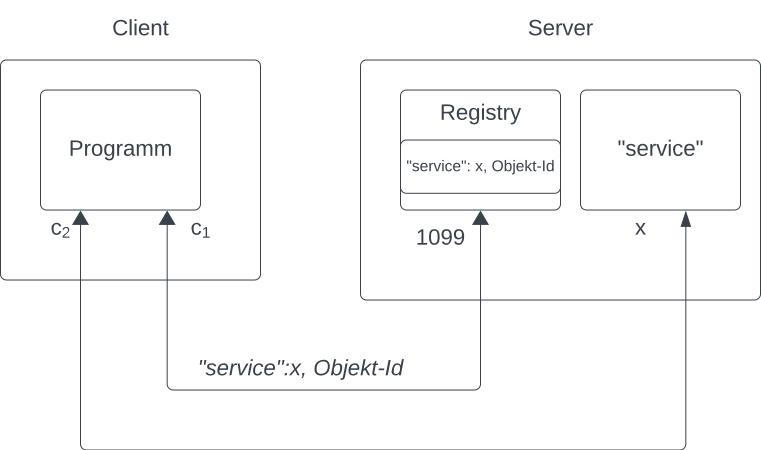
\includegraphics[scale=0.5]{chapters/fopt5/img/rmi/registry}
    \caption{Ein Client fragt den Eintrag der Registry für ``service`` ab und erhält über den Port des Client-Rechners $c_1$ die Erreichbarkeitsinformationen, die u.a. aus einer Portnummer $x$ und einer Objekt-Kennung bestehen.
    Antworten auf seine Anfragen werden daraufhin an seinen Port $c_2$ gesendet. (Quelle: in Anlehnung an \cite[324, Bild 6.5]{Oec22})}
    \label{fig:registry}
\end{figure}

Die \textbf{Registry} lässt sich auch aus dem Programm heraus starten\footnote{
``Class LocateRegistry``: \url{https://docs.oracle.com/en/java/javase/21/docs/api/java.rmi/java/rmi/registry/LocateRegistry.html} - abgerufen 2.2.2024
}:

\begin{minted}[mathescape,
    linenos,
    numbersep=5pt,
    gobble=2,
    frame=lines,
    framesep=2mm]{java}
    java.rmi.registry.LocateRegistry.createRegistry(port:int):Registry
\end{minted}\\

Der zurückgegebene Typ implementiert \code{java.rmi.registry.Registry} und besitzt dieselben Methoden wie \code{java.rmi.Naming}\footnote{was aber nicht heißt, dass \textit{Naming} auch \textit{Registry} implementiert - die Methoden von \textit{Naming} sind allesamt statisch.
}.\\
$\rightarrow$ Entweder wird die Registry nur in einem Server gestartet, oder weitere Registries müssen eigene, unterschiedliche Portnummern enthalten.

\subsection*{Eigene Notizen}

Länger andauernde Aufträge an ein Remote-Objekt sollten über Threads realisiert werden.\\

\noindent
Muss eine UI während / infolgedessen aktualisiert werden, sollte diese UI-Aktualisierung über \code{javafx.application.Platform.runLater()} stattfinden (\textbf{JavaFX Application Thread}).


\section{Parallelität bei RMI-Methodenaufrufen}

Ein \textbf{Skeleton} ist ein paralleler \textbf{TCP-Server} (vgl.\cite[329]{, Oec22}).\\

\begin{tcolorbox}
    Identität und Gleichheit von zwei \textbf{Stubs}:\\
    \noindent
    Rückgabewert von \code{Naming.lookup(...)} führt bei Objektvergleich mittel $==$zu \code{false}, wenn ein Stub für ein und denselben Namen zweimal angefordert wird, \code{equals()} hingegen zu \code{true}.\\

    $\rightarrow$ \textbf{Stub-Objekte} sind in diesem Fall nicht ``identisch``, aber wenn sie auf dasselbe \textbf{RMI-Objekt} zeigen, werden sie als ``gleich`` betrachtet.\\

    ``Zwei Stub-Objekte sind genau dann gleich, wenn sie eine Referenz auf dasselbe Objekt in der Ferne repräsentieren.`` (\cite[347]{Oec22})
\end{tcolorbox}\\

\noindent
Wird ein \textbf{Stub} angefordert, der eine asynchrone Operation ausführt, und dieser Stub wird in einen Thread ausgelagert, verhält sich der Stub \textit{intelligent}:

\begin{itemize}
    \item wenn mehrere Threads erzeugt werden, und ``parallel`` gearbeitet wird, werden die Operationen auch parallel ausgeführt, und zwar indem mehrere Verbindungen aufgebaut werden (dadurch werden auf Server-Seite mehrere Threads erzeugt).
    \item wird auf Client-Seite keine parallele Ausführung durch die Erzeugung von Threads erzwungen, findet die Abarbeitung der Operation(en) sequentiell statt, es wird dann auch nur eine Verbindung dafür aufgebaut.
    \item ein einzelner Stub ist also auch dazu in der Lage, parallele Aufrufe auf dem Server zu erzeugen
\end{itemize}\\


\begin{tcolorbox}
    Methodenaufrufe auf ein RMI-Objekt finden parallel statt durch mehrere Clients - beim Zugriff auf gemeinsame Daten muss entsprechend synchronisiert werden\footnote{
        s.a. ``3.2 Thread Usage in Remote Method Invocations``: Die Spezifikationen scheinen hier keinen Hinweis darauf zu geben, dass es eine Garantie für die Threads gibt. Steht das im Widerspruch zu der Aussage im Buch (\cite[330]{Oec22})? \url{https://docs.oracle.com/en/java/javase/21/docs/specs/rmi/arch.html#thread-usage-in-remote-method-invocations} - abgerufen 2.2.2024
    }.
\end{tcolorbox}

\begin{tcolorbox}[colback=red!20,color=white,title=Anmerkung]
    Die Spezifikationen unter ``3.2 Thread Usage in Remote Method Invocations``\footnote{
        \url{https://docs.oracle.com/en/java/javase/21/docs/specs/rmi/arch.html#thread-usage-in-remote-method-invocations} - abgerufen 2.2.2024
    } geben keinen Hinweis darauf, dass es eine Garantie für die Threads gibt, im Gegensatz zu~\cite[330]{Oec22}.
\end{tcolorbox}

\section{Wertübergabe für Parameter und Rückgabewerte}

Bei \textbf{RMO} können Objektparameter oder Objektrückgabewerte als \textbf{Wert} oder \textbf{Referenz} übergeben werden.\\

\noindent
Bei der Übergabe als Wert wird eine Kopie des Objektes erzeugt, und zwar rekursiv bei gleichzeitiger Vermeidung von Zyklen.\\

\noindent
Diese Kopie wird dann auf dem Server in der entsprechenden Methode aufgerufen:

\begin{tcolorbox}
    Damit ein Objekt auf einen Server übertragen werden kann, muss es \code{java.io.Serializable} implementieren.
\end{tcolorbox}

\begin{itemize}
    \item wird das Objekt auf dem Server geändert, ändert sich nur \ul{dieses} Objekt auf dem Server, nicht aber das auf dem Client.
    \item \ul{als Rückgabewert} kann das geänderte Objekt aber vom Client verwendet werden
\end{itemize}

Datenstrukturen werden unter Verwendung von \code{java.io.Serializable} serialisiert {bzw.} deserialisiert; Objekte, die als ``Foge von Bytes`` serialisiert werden sollen, müssen dabei \code{java.io.Serializable} implementieren  - das gilt auch für die Objekte, die mit dem zu serialisierenden Objekt assoziiert sind (vgl.~\cite[332]{Oec22}).\\

\noindent
Bei \textbf{RMI} findet die Serialisierung automatisch statt; möchte man {bspw.} ein Objekt serialisieren und in eine Datei schreiben, muss man die Logik zum Speichern/Lesen des Objektes selber implementieren\footnote{
auch wenn das Beispiel nicht viel Code enthält, sollte klar sein, dass das (De)Serialisieren bei RMI automatisch geschieht und bei Abfrage des Rückgabewerts/ Übergabeparameters bereits erfolgt ist, ohne dass zusätzliche Methoden aufgerufen werden müssen.
}, wie folgendes Beispiel zeigt:\\

\begin{minted}[mathescape,
    linenos,
    numbersep=5pt,
    gobble=2,
    frame=lines,
    framesep=2mm]{java}

    // schreiben
    FileOutputStream fos = new FileOutputStream(fileName);
    ObjectOutputStream output = new ObjectOutputStream(fos);
    // hier findet das serialisieren statt
    output.writeObject(obj);
    output.flush();

    //lesen
    FileInputStream fis = new FileInputStream(fileName);
    ObjectInputStream input = new ObjectInputStream(fis);
    // hier findet das de-serialisieren statt
    ConcreteObject obj = (ConcreteObject)input.readObject();
\end{minted}\\

\noindent
Im Wesentliche wird bei der Serialisierung der Zustand eines Objektes gespeichert, was vor allem durch die aktuellen Werte der Attribute des Objektes beschrieben wird.\\

\noindent
Attribute, die bei der Serialisierung nicht berücksichtigt werden sollen, können durch den Feld-Modifizierer \code{transient} entsprechend gekennzeichnet werden\footnote{
vgl. ``8.3.1.3. transient Fields`` \url{https://docs.oracle.com/javase/specs/jls/se21/html/jls-8.html#jls-8.3.1.3} - abgerufen 2.2.2024
}


\begin{tcolorbox}
    Ein Objekt wird als Wert übergeben, wenn es serialisierbar ist und nicht exportiert ist.
\end{tcolorbox}


\section{Referenzübergabe für Parameter und Rückgabewerte}

Bei \textbf{RMI} werden Parameter und Rückgabewerte entweder als Wert oder als Referenz übergeben.\\

\noindent
Als \textbf{Wert} i.d.R. nur, wenn eine Klasse \code{Serializable} implementiert, ansonsten hat die \textbf{Referenzübergabe} Vorrang, falls ein Objekt einer Klasse \textbf{exportiert} ist (bspw. weil seine Klasse von \code{UnicastRemoteObject} abgeleitet ist).\\



\begin{tcolorbox}
    RMI-Objekte implementieren die \code{Remote}-Schnittstelle und sind aus \code{UnicastRemoteObject} abgeleitet.
\end{tcolorbox}\\

\noindent
Für ein Objekt, das bei \textbf{RMI} als Referenz übergeben wird, wird ein \textbf{Stub} erzeugt, hierzu muss aber nicht extra das betreffende Objekt in einer Registry registriert sein - der Server erhält das \code{Stub}-Objekt nicht über die Registry!\\

\noindent
Eine Übergabe als Referenz ist bspw. dann sinnvoll/ notwendig, wenn der Server auf dem Client Daten ändern muss\footnote{als Beispiel die in Abschnitt 6.5 des Buches vorgestellte Chat-Anwendung - der Server ruft die \textbf{print}-Methode der Clients auf, Clients aktualisieren daraufhin ihr UI mit dem Übergabeparameter... (vgl.~\cite[Listing 6.22, Listing 6.24]{Oec22})}.\\

\noindent
Damit eine Übergabe als Referenz funktioniert, muss die zu übergebende Objektsinstanz vom Typ \code{Remote }sein.\\

\noindent
Werden \code{UnicastRemoteObjekte} genutzt, erstellen diese zur \textbf{TCP}-Kommunikation Threads.
Deshalb sollte darauf geachtet werden, dass diese Threads beendet sind, bspw. durch einen Aufruf von \code{System.exit(0)}, wenn es zu einem ``kontrollierten`` Programmende kommt\footnote{s. \cite[352]{Oec22}; außerdem ``Shutdown Sequence``: \url{https://docs.oracle.com/en/java/javase/21/docs/api/java.base/java/lang/Runtime.html#shutdown} - abgerufen 2.2.2024
}.\\

\begin{tcolorbox}
    \item Ein Objekt, das eine \textbf{RMI}-Schnittstelle implementiert und von \code{UnicastRemotObject} abgeleitet ist und \textbf{serialisierbar} ist, wird trotzdem als \textbf{Referenz} übergeben.\\

    \noindent
    \textbf{Referenzübergabe} hat Vorrang vor \textbf{Wertübergabe}.
\end{tcolorbox}

\subsection*{Eigene Notizen}

\noindent
Eine \code{ArrayList} nutzt in ihren Methoden bei Objekten \code{equals} zum Vergleich der enthaltenen Elemente\footnote{
    s. \url{https://docs.oracle.com/en/java/javase/21/docs/api/java.base/java/util/ArrayList.html#equals(java.lang.Object)} - abgerufen 2.2.2024
}.\\

\noindent
Über einen \code{Iterator} können bedenkenlos Objekte entfernt werden, ohne, dass es zu einer \code{ConcurrentModificationExcepion} kommt\footnote{ein Iterator kennt \textit{remove()}, aber kein \textit{add()}. S. \url{https://docs.oracle.com/en/java/javase/21/docs/api/java.base/java/util/Iterator.html#remove()} - abgerufen 2.2.2024}.\\


\noindent
Chatbeispiel: Dem Abmelden von Clients sollte genug Zeit eingeräumt werden - funktioniert das Abmelden nicht richtig, entfernt der Server die fehlerhaften Clients allerdings ohnehin wegen der abgefangenen Exception - s. \cite[345, Listing 6.22]{Oec22}.
%fopt6
\usepackage{lstmisc}\chapter{Webbasierte Anwendungen mit Servlets und JSF}

Bei webbasierten Anwendungen wird die Client-Seite durch einen Web-Browser realisiert, auf der Server-Seite wird ein Web-Server wie bspw. \textit{Apache Tomcat}\footnote{
    \url{https://tomcat.apache.org} - abgerufen 3.2.2024
} benutzt.\\

\noindent
Der Web-Server liefert statische Dateien aus oder Seiten, die Programmcode enthalten, der auf dem Client ausgeführt wird (bspw. \textit{JavaScript}).\\

\noindent
Der Client kann auch über den Server ausgeführte Programme anfordern, die entsprechende Daten für den Client generieren, wie bspw. Servlets.\\

\noindent
Um mit einem Server zu kommunizieren, baut der Client über \textbf{TCP} eine Verbindung mit dem Server auf:\\
Über das \textbf{HTTP-Protokoll}\footnote{
Bestandteilt der Anwendungsschicht - s. \url{https://en.wikipedia.org/wiki/HTTP} - abgerufen 3.2.2024
} werden dann Anfragen und Antworten zwischen Client und Server verhandelt; Antworten können über auf dem Server laufende Programme dynamisch generierte Seiteninhalte sein.\\

\noindent
\textbf{HTTP} (\textit{HyperTextTransferProtocol}) ist ein ASCII-Protokoll auf Schicht 5 und für die Vermittlung webbasierter Dienste gedacht.

\begin{figure}
    \centering
    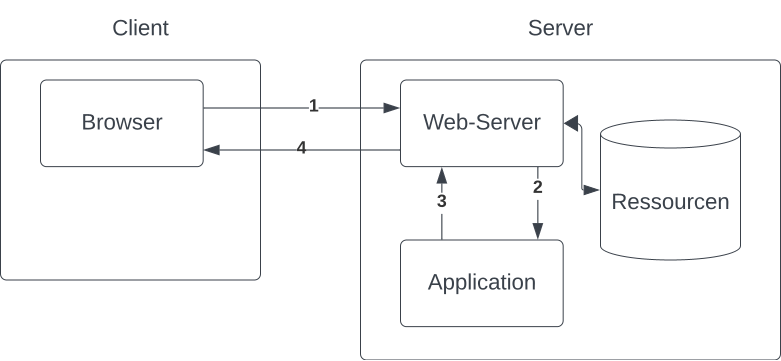
\includegraphics[scale=0.5]{chapters/fopt6/img/clientserver}
    \caption{Der Client erstellt über den Webbrowser eine TCP-Verbindung zu dem Webserver, wobei die Adressinformationen in der URL festgelegt sind. Der Webserver kann nun in seiner Antwort sowohl statische Ressourcen als auch dynamisch generierte Daten bereitstellen. Syntax und Semantik der Anfrage und Antwort ist über das HTTP-Protokoll definiert (Quelle: in Anlehnung an \cite[402, Bild 8.1]{Oec22})}
    \label{fig:clientserver}
\end{figure}

\subsection{GET}

Über eine \textbf{URL} (\textit{Universal Resource Locator}\footnote{
s. \url{https://en.wikipedia.org/wiki/URL} - abgerufen 3.2.2024
}) wird über den Browser eine Ressource angefordert.


\begin{tcolorbox}
    Eine \textbf{URL} ist eine \textbf{URI} (\textit{Uniform Resource Identifier}\footnote{
        s. \url{https://en.wikipedia.org/wiki/Uniform_Resource_Identifier} - abgerufen 3.2.2024
    }) und enthält u.a. weitere Informationen zur Lokalisierung der Ressource - bspw. durch die Angabe des Protokolls, über das die Ressource beschafft werden soll\footnote{s. ``RFC 3986 - 1.1.3.  URI, URL, and URN``: \url{https://datatracker.ietf.org/doc/html/rfc3986#section-1.1.3} - abgerufen 3.2.2024}.
\end{tcolorbox}

Der an den Server übermittelte \textbf{GET}-Request besteht aus der Angabe der angeforderten Ressource und dem Protokoll, das verwendet wird:

\begin{minted}[]{http}
GET /resource.html HTTP/1.1
\end{minted}
\\

$\rightarrow$ Ein \textbf{GET}-Request besteht aus beliebig vielen Zeilen.
Mit einer Leerzeile wird das Ende des Request angezeigt.\\

\noindent
eine \textbf{HTTP-Response} enthält wieder Kopfdaten (\textbf{Header}) und den \textbf{Body}, der leer sein kann.\\
Header und Body sind durch eine Leerzeile voneinander getrennt\footnote{
    s. \url{https://www.rfc-editor.org/rfc/rfc7230#section-3} - abgerufen 3.2.2024
}.\\
Weitere Leerzeilen im Body haben keine weitere Bedeutung für das Protokoll und gehören zum Inhalt der angeforderten Ressource.\\

\noindent
Der Client kann weitere Daten anfordern, bspw. wenn in der ausgelieferten HTML-Seite Bilder oder andere statische Ressourcen vorkommen.\\
Bei \textbf{HTTP/1.0} muss der Client für jede Ressource eine neue \textbf{TCP}-Verbindung aufbauen.\\
Nutzt der Client hingegen \textbf{HTTP/1.1}, hält der Server genau diese Verbindung offen.
Über diese Verbindung kann der Client weitere Daten anfordern.

\begin{itemize}
    \item Bei der Verwendung von \textbf{HTTP/1.1} muss außerdem in der zweiten Zeile der Anfrage der Zielhost stehen, damit ein Server, der {ggfl.} mehrere Domains hostet, die Anfrage an die richtige Domain weiterleitet\footnote{s. ``RFC 7320 - 5.4.  Host``: \url{https://www.rfc-editor.org/rfc/rfc7230#section-5.4} - abgerufen 3.2.2024}.
    \begin{minted}[]{http}
GET /index.php HTTP/1.1
Host: www.conjoon.org
    \end{minted}
    \item Wird der Header \textit{Connection: keep-alive}\footnote{
    s. ``RFC 2068 - 19.7.1 Compatibility with HTTP/1.0 Persistent Connections``: \url{https://www.rfc-editor.org/rfc/rfc2068#section-19.7.1} - abgerufen 3.2.2024
    } mitgesendet, teilt der Client dem Server mit, dass die Verbindung zum Herunterladen weiterer Daten geöffnet bleiben soll.
    \item Bei einer HTTP-Response weist die Antwort-Zeile \textit{Connection: close} daraufhin, dass die Verbindung nicht persistent ist und mit der Bearbeitung der Antwort geschlossen wird\footnote{
    s. ``RFC 2068 - 14.10 Connection``: \url{https://www.rfc-editor.org/rfc/rfc2068#section-14.10} - abgerufen 3.2.2024
    }.
\end{itemize}

\subsection{Formulare in HTML}

\textit{<form>...</form>} wird für Formulare in HTML genutzt, in \textit{action} steht die URL, an der die Formulardaten gesendet werden sollen, mit \textit{method} kann man die HTTP-Methode angeben, die zum Senden des Formulars genutzt werden soll\footnote{
s. ``<form>: The Form element``:\url{https://developer.mozilla.org/en-US/docs/Web/HTML/Element/form} - abgerufen 3.2.2024
}.\\

\noindent
\textbf{radio}-inputs erhalten alle dasselbe \textit{name}-Attribut, um sie zu einer gruppe zusammenzuführen.\\

\noindent
Fehlt für eine \textbf{checkbox} die Selektion, wie sie bei der Übertragung der Formulardaten nicht mitverschickt.
Ist das \textit{value}-Attribut für die Checkbox gesetzt und wurde die Checkbox selektiert, enthalten die Request-Daten den Inhalt von \textit{value}, ansonsten standardmäßig den Wert \textit{on}:

\blockquote[{\url{https://developer.mozilla.org/en-US/docs/Web/HTML/Element/input/checkbox} - abgerufen 3.2.2024, Hervorherbungen ausgelassen}]{
    If the value attribute was omitted, the default value for the checkbox is on, so the submitted data in that case would be subscribe=on.
}

\subsection{POST}

Nutzt man \textbf{GET} zur Übermittlung von Formulardaten, werden die Daten als Query-String an die URL gehangen.\\

\noindent
\textbf{POST} schickt die Formulardaten im Body an die in \textit{action} angegebene URL.

\begin{itemize}
    \item Vorteile \textbf{GET}: Formulardaten können mit der URL gespeichert werden, bei \textbf{POST} geht das nicht, da diese im Body verborgen sind
    \item Nachteile \textbf{GET}: bei \textbf{GET} ist die Länge der eingegebenen Formulardaten begrenzt, bei \textbf{POST} nicht.
    \begin{tcolorbox}[colback=red!20,color=white,title=Anmerkung]
    Die Aussage bzgl. der Begrenzung von \textbf{GET/POST} findet sich in \cite[409]{Oec22}.\\
    Tatsächlich ist die Länge nicht begrenzt per Spezifikation\footnote{``RFC 7230 - 3.1.1.  Request Line``: \url{https://datatracker.ietf.org/doc/html/rfc7230#section-3.1.1} - abgerufen 3.2.2024}. \\
    Es wird aber empfohlen, Request URIs abzuweisen, die zu lang sind\footnote{siehe bspw. ``RFC 2616 - 10.4.15 414 Request-URI Too Long``: \url{https://datatracker.ietf.org/doc/html/rfc2616#section-10.4.15} - abgerufen 3.2.2024
    }.\\
    Auch für \textbf{POST} wird in den Spezifikationen keine max. Länge vorgegeben.
    Allerdings kann die max. akzeptierte Länge des Bodys eines POST-Requests durch den Web-Server begrenzt werden\footnote{
        ``RFC7231 - 6.5.11.  413 Payload Too Large``: \url{https://www.rfc-editor.org/rfc/rfc7231#section-6.5.11} - abgerufen 3.2.2024
    }.\\
    Beides ist sinnvoll, um einer Überlastung des Webservers durch zu große Anfrage-Längen vorzubeugen.
    \end{tcolorbox}
\end{itemize}

\subsection{Format von HTTP-Anfragen und -Antworten}

Eine HTTP-Anfrage hat grundsätzlich folgende Struktur\footnote{
Es ist grundsätzlich möglich, bei GET-Requests den Body mitzuschicken.
    Allerdings rät RFC 9110 davon ab: ``A client \textbf{SHOULD NOT} generate content in a GET request unless it is made directly to an origin server that has previously indicated, in or out of band, that such a request has a purpose and will be adequately supported. An origin server \textbf{SHOULD NOT} rely on private agreements to receive content, since participants in HTTP communication are often unaware of intermediaries along the request chain.`` (Hervorhebungen i.O., \url{https://www.rfc-editor.org/rfc/rfc9110#section-9.3.1-6} - abgerufen 3.2.2024)
}:

\begin{minted}[]{text}
<methode> <uri> HTTP/<version>
<headername>: <headerwert>
...
<headername>: <headerwert>
<newline>
<body>
\end{minted}

Die Antwort sieht i.A. folgendermaßen aus:

\begin{minted}[]{text}
HTTP/<version> <StatusCode> <StatusText>
<headername>: <headerwert>
...
<headername>: <headerwert>
<newline>
<body>
\end{minted}

\subsection*{``Content-Length`` Header}
Bei \textbf{POST} nutzt der Server die Verbindung, die der Client zur Anfrage aufgebaut hat, um die Antwort zu senden.\\
Der Server muss wissen, wann er den kompletten Datenteil gelesen hat, bevor er mit der Antwort beginnt.\\
Bis zum Verbindungsende kann nicht gelesen werden, sonst kann keine Antwort gesendet werden.\\
Trennzeichen sind für den Body nicht ausgemacht.\\
Nach $n$-Zeichen, die der Client im Header über \textbf{Content-Length} spezifiziert, geht der Server davon aus, dass die Anfrage nach der Leerzeile (Trennzeichen Header / Body) genauso viele Daten enthält.\\
Sind diese $n$ Daten gelesen, beginnt der Server mit der Aufbereitung der Antwort an den Client\footnote{
s.a. Skript FOPT6 Übung 14.2
}.



%
\begin{appendices}
    
\begin{appendices}
    
\begin{appendices}
    \input{chapters/Anhang/Zusatzaufgaben/index}
    \input{chapters/Anhang/Klausuren/ws13}
    \input{chapters/Anhang/Klausuren/ws15-16}
    \input{chapters/Anhang/Klausuren/ws16-17}
    \input{chapters/Anhang/Klausuren/ss19}
    \input{chapters/Anhang/Präsenzphase/index}

\end{appendices}

    \chapter{WS13}\label{ch:klausurws13}

\section{Aufgabe 1}
\subsection{Lösungsvorschlag}


\begin{minted}[mathescape,
    linenos,
    numbersep=5pt,
    gobble=2,
    fontsize=\small,
    frame=lines,
    framesep=2mm]{java}
    class Zahlenschloss {

        private int[] kombination;

        private int[] state;

        private boolean opened = false;

        public Zahlenschloss(int[] kombination) {
            this.kombination = kombination;
            this.state = new int[kombination.length];
        }

        public int anzahlRaedchen() {
            return kombination.length;
        }

        public synchronized int lesen(int radnummer) {
            return state[radnummer];
        }

        public synchronized void drehen(int radnummer, int zahl) {

            state[radnummer] = zahl;
            opened = true;
            for (int i = 0; i < anzahlRaedchen(); i++) {
                if (lesen(i) != kombination[i]) {
                    opened = false;
                    break;
                }
            }

            if (opened) {
                this.notify();
            }
        }

        public synchronized void warten() {

            while (!opened) {
                try {
                    this.wait();
                } catch (InterruptedException ignored) {}
            }
        }
    }
\end{minted}\\


\subsection{Anmerkung und Ergänzungen}

\begin{itemize}
    \item Es wird eine Wartebedingung benötigt, und zwar für die Methode \code{warten()}; ankommende Threads werden
    in die Warteschlange des Zahlenschloss-Objektes geschickt, wenn \code{opened} auf false gesetzt ist, ansonsten
    verlassen diese direkt die Methode wieder.\\
    Die Methode \code{drehen} benötigt keine separate Wartebedingung.
    Es reicht aus, sicherzustellen, dass das Zahlenschloss nicht gleichzeitig von anderen Threads benutzt werden kann:
    Die Methode \code{drehen} ist hierfür synchronisiert, damit das Zahlenschloss {insg.} immer nur eine Zustandsänderung
    erfährt - es sind andere Implementierungen möglich, in denen das Zahlenschloss dann von mehreren Threads gleichzeitig
    genutzt werden darf, wenn sich die Zugriffe anhand der ``Ziel``-\code{radnummer} unterscheiden, {bspw.} durch Mutex-Semaphore,
    die pro Radnummer verwendet werden\footnote{
        der gleichzeitige Zugriff auf unterschiedliche Arrays-Indizes ist erlaubt, s. `´17.4.1. Shared Variables``: \url{https://docs.oracle.com/javase/specs/jls/se21/html/jls-17.html#jls-1.4.1} - abgerufen 14.2.2024
    }.
    \item Es gibt nur eine Wartebedingung, von daher sollte \code{notify()} genügen.\\
    Wenn wir allerdings davon ausgehen, dass mehrere Threads über die Methode \code{warten()} in die Warteschlange des Objektes eingereiht worden sind,  sollte \code{notifyAll()} verwendet werden (siehe hierzu auch Abschnitt \ref{subsec:notifyAll}).
    Dennoch ist nicht garantiert, dass auch alle Threads aus der Warteschlange gelangen, denn es kann sein, dass ein anderer Thread die Methode \code{drehen()} betritt, dort die
    Zahlenkombination ändert und \code{opened} wieder auf \code{false} gesetzt wird. \\
    Ein anderer Thread, der nun in  \code{warten()} an die Reihe kommt, überprüft die Wartebedingung, und wird wieder in die Warteschlange eingereiht.
    Es ist also durchaus möglich, dass ein Thread nicht mehr aus der Methode \code{warten()} herauskommt.\\
    Dies könnte bspw. dadurch verhindert werden, dass die Threads in eine Queue gepackt werden, und in \code{drehen()} eine Wartebedingung eingefügt wird, die erst erfüllt ist,
    wenn die Queue geleert wurde oder aus ihr entnommen wurde, in der Reihenfolge, in der die Threads in die Queue eingereiht worden sind (\textit{FIFO}) (s. a. Abschnitt~\ref{subsec:readerwriterproblem}).
    \item Bei der Teilaufgabe mit der Schleife muss die komplette Schleife synchronisiert werden, was man durch ein \code{synchronized}-Statement erreicht\footnote{siehe Abschnitt~\ref{subsec:synchronizedstatement}.}
    \begin{minted}[mathescape,
        linenos,
        numbersep=5pt,
        gobble=2,
        fontsize=\small,
        frame=lines,
        framesep=2mm]{java}
        synchronized (zk) {
            for (int i = 0; i < anzahlRaedchen; i++) {
                System.out.println(zk.lesen(i));
            }
        }
    \end{minted}
    Ansonsten läuft man Gefahr, dass sich nach Auslesen der 1. Position der Wert von Position 2 geändert hat und dadurch eine
    Zahlenkombination ausgegeben wird, die es nicht gegeben hat:
    \begin{enumerate}
        \item $K\coloneqq[0, 0, 0]$
        \item Position $K_0$ wird ausgelesen und liefert $0$.
        \item Thread ändert $K_0$ zu $1$ $\implies K\coloneqq[1, 0, 0] $.
        \item Thread ändert $K_1$ zu $2$ $\implies K\coloneqq[1, 2, 0] $.
        \item Thread ändert $K_2$ zu $3$ $\implies K\coloneqq[1, 2, 3] $.
        \item Positionen $K_1$ und $K_2$ werden ausgelesen und liefern: $2, 3$
        \item Ausgabe: $0, 2, 3$ - diese Kombination hat es in dem Fall aber tatsächlich nicht gegeben.
    \end{enumerate}
\end{itemize}

\begin{tcolorbox}[colback=red!20,color=white,title=Anmerkung]
    Die Methode \code{lesen()} als \code{synchronized} zu markieren könnte man sich vlt. sparen, wenn man davon ausgeht,
    dass die Methode ohnehin in einem \code{synchronized}-Statement verwendet wird, um alle Rädchen abzulesen.\\
    Mehrere Threads können also nicht parallel auf unterschiedliche Positionen des Feldes zugreifen, wenn die Methode
    synchronisiert ist.\\
    Allerdings ist sowohl das Skript als auch das Buch recht klar, was in dieser Situation geschehen muss (s. Skript Fopt1/2, S. 9, außerdem \cite[31, Abschnitt 2.3.6]{Oec22}): Es muss (in diesem Kurs) immer \code{synchronized} verwendet werden, wenn gleichzeitig
    Daten geschrieben und gleichzeitig diese Daten gelesen werden sollen - und eine andere Implementierung, bei der die
    einzelnen Positionen ``gelocked`` sind, so dass ein gleichzeitiger Zugriff auf unterschiedliche Rädchen möglich ist, war nicht gefordert.\\
    Ggfl. würde in anderen Implementierungen der Einsatz von \code{AtomicReferenceArray}\footnote{s. \cite[157 ff.]{Oec22}
    s. ``Class AtomicReferenceArray<E>``: \url{https://docs.oracle.com/en/java/javase/21/docs/api/java.base/java/util/concurrent/atomic/AtomicReferenceArray.html} - abgerufen 15.2.2024
    } Sinn machen, aber das Lehrmaterial ist bereits sehr eindeutig bzgl. der Verwendung von \code{synchronized}.
\end{tcolorbox}



\section{Aufgabe 3}
\subsection{Lösungsvorschlag}

\subsection*{Statische Parallelität}
Statische Parallelität erlaubt es einem Server, eine \textit{fixe} Anzahl von Verbindungen gleichzeitig zu bedienen.\\
Hierbei wird ein Feld von Threads erstellt, wobei jeder Thread das \code{ServerSocket}-Objekt als Referenz übergeben bekommt.
In der \code{run()}-Methode wird dann über \code{accept()} in einer Endlosschleife auf eingehende Verbindungen gewartet, die dann so lange bedient werden, bis sich ein Client wieder abmeldet (oder eine andere Abbruchbedingung erfüllt ist, wie z.B. ein \code{SocketTimeout}).\\
Das sich ein Client abmeldet, bekommt man bspw. dadurch mit, dass \code{null} beim Lesen von einer Nachricht des Clients zurückgegeben wird (vgl. \cite[286]{Oec22}. \\
Siehe Abschnitt~\ref{sec:seqparserver} für ein Implementierungsbeispiel.



\subsection*{Dynamische Parallelität}

Bei der \textbf{Dynamischer Parallelität} erzeugt der Server für jede Verbindung einen neuen Thread, der so lange läuft, bis der Client die Verbindung wieder trennt.\\
Die Anzahl der Threads ändert sich dadurch laufend.\\
Wird die max. Anzahl erlaubter Threads nicht kontrolliert, kann es zu einer Überlastung des Server-Rechners kommen (bspw. durch einen Denial-of-Service-Angriff.)\\

\noindent
I.d.R. ist eine Mischform aus beidem geeignet, um mehrere Clients gleichzeitig bedienen zu können, und dabei nicht Gefahr zu laufen, durch dynamisches, unbegrenztes Wachstum der Anzahl der Threads überlastet zu werden.

    \chapter{WS13}\label{ch:klausurws5-16}

\section{Rechteck-Scroll (SS15 Aufgabe 2)}

Aufgabenstellung unklar.\\
Mögliche Implementierung unter \url{https://github.com/ThorstenSuckow/fopt/tree/main/src/main/java/klausurvorbereitung/foptws1516/MouseDragsSquareDemo}.

\section{Rechteck-Scroll (WS15/16 Aufgabe 1)}

Aufgabenstellung unklar.\\
Mögliche Implementierung unter \url{https://github.com/ThorstenSuckow/fopt/tree/main/src/main/java/klausurvorbereitung/foptws1516/MaxWeightDemo}.\\

\noindent
Es gibt nur eine Warteschlange für Threads in \code{use()}, es gibt keine Wartebedingung in \code{dontUse()} und damit auch keine weitere Warteschlange.\\
Es sind durch die Zugriffe auf unterschiedliche Indizes allerdings mehrere Wartebedingungen vorhanden, weshalb hab \code{notifyAll()} nutzen sollte,
sobald ein Zugriff auf ein Feld nach Aufruf von \code{dontUse} wieder möglich wird.\\
Ansonsten bestünde die Gefahr, dass bei dem Einsatz von \code{notify()} ein wartender Thread nicht geweckt wird, obwohl er weiterlaufen könnte:\\
Angenommen, das Feld $F$ hat eine Länge von $3$, das \code{maxWeight} ist mit $2$ konfiguriert.
Thread $t_1$ mit einer Laufzeit von $200\ sek$ bekommt Zugriff auf $F_0$, setzt $currentWeight$ auf $1$.\\
Thread $t_2$ mit einer Laufzeit von $1\ sek$ möchte auf $F_1$ zugreifen, setzt $currentWeight=2$ in die Warteschlange.\\
Thread $t_3$ meldet Zugriff auf $F_0$ an und gelangt in die Warteschlange.\\
Thread $t_4$ meldet Zugriff auf $F_1$ an und gelangt in die Warteschlange.\\
Thread $t_2$ ist mit der Bearbeitung von $F_1$ fertig, $currentWeight$ wird auf $1$ gesetzt, \code{notify()} wird aufgerufen.\\
Thread $t_3$ wird aus der Warteschlange geholt, kann aber nicht weiterarbeiten, da $F_0$ noch durch den länger dauernden $t_1$ blockiert ist, und kommt wieder in die Warteschlange.\\

\noindent
Offensichtlich hätte in dem Beispiel \code{notifyAll()} dazu geführt, dass auch $T_4$ seine Wartebedingung hätte überprüfen können, und hätte so Zugriff auf $F_1$ bekommen.
Stattdessen muss nun gewartet werden, bis das nächste \code{notify()} aufgerufen wird, oder ein neu ankommender Thread $F_1$ belegt.

    \chapter{WS16-17}\label{ch:klausurws16-17}

\section{Aufgabe 1}
\subsection{Lösungshinweis}

Die erste Aufgabe verdeutlicht, was bei einem \code{notifyAll()} und unsauber gesetzten Wartebedingungen passieren kann.\\
Sei folgender Quellcode gegeben:


\begin{minted}[mathescape,
    linenos,
    numbersep=5pt,
    gobble=2,
    fontsize=\small,
    frame=lines,
    framesep=2mm]{java}
    class Cond1AndCond2 {

        private boolean cond1;
        private boolean cond2;

        public synchronized void setCond1(boolean c) {
            cond1 = c;
            notifyAll();
        }

        public synchronized void setCond2(boolean c) {
            cond2 = c;
            notifyAll();
        }

        public synchronized void cond1AndCond2() {
            while(!cond1) {
                try {
                    wait();
                } catch(InterruptedException e) { }
            }

            while(!cond2) {
                try {
                    wait();
                } catch(InterruptedException e) {}
            }
            System.out.println("cond1 and cond2:" + cond1 + " " + cond2);
        }
    }
\end{minted}\\

Man sollte auf den ersten Blick meinen, dass \code{cond1} und \code{cond2} beide \code{true} sein müssen, damit die Ausgabe erfolgt.\\
Tatsächlich ist es aber so, dass es in der Methode zwei unterschiedliche Wartebedingungen gibt.\\
Die erste Wartebedingung schickt einen Thread in die Warteschlange, wenn \code{cond1 == false} gilt.\\
Setzt ein anderer Thread über \code{setCond1(true)} das Attribut entsprechend auf \code{true}, bewirkt der nachfolgende Aufruf von \code{notifyAll()}, dass alle \textit{wartenden} Threads aus der Warteschlange entfernt werden und erneut um eine Sperre des Objektes konkurrieren.\\
Erhält ein entsprechender Thread $t_w$ die Sperre auf das Objekt und kann seine \textit{while-wait-Schleife} verlassen, kann es vorkommen, dass er erneut in die Warteschlange eingereiht wird, wegen der nachfolgenden Wartebedingung \code{cond2 == false}.\\
Angenommen, ein weiterer Thread ruft nun \code{setCond2(true)} auf, und $t_w$ kommt aus der Warteschlange und konkurriert erneut und um die Sperre des Objektes, dann kann es vorkommen, das ein anderer Thread zunächst die Sperre erhält, \code{cond1} wieder auf \code{false} setzt, dann erhält $t_w$ die Sperre, überprüft die Wartebedingung \code{cond2 == false}.\\
Wegen \code{cond2} gelangt er aus der \textit{while-wait-Schleife} und die Ausgabe erfolgt - da zwischenzeitlich \code{cond1} wieder auf \code{false} gesetzt wurde, ist die erwartete Ausgabe nicht \code{true true}, sondern \code{false true} (s. Abbildung \ref{fig:cond1cond2}).\\

\begin{figure}
    \centering
    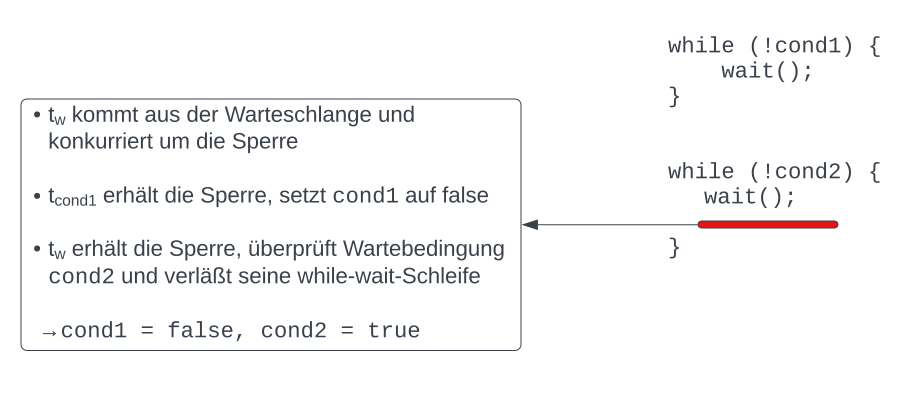
\includegraphics[scale=0.4]{chapters/Anhang/Klausuren/img/cond1cond2}
    \caption{in den rot markierten Bereich konkurriert $t_w$ um die Sperre des Objektes - wenn durch einen anderen Thread, der vor $t_w$ die Sperre erhält, \textit{cond1} auf \textit{false} gesetzt wird, stimmt die Ausgabe nicht mit der erwarteten überein. (Quelle: eigene)}
    \label{fig:cond1cond2}
\end{figure}

\noindent
Die korrekte Wartebedingung sollte lauten:

\begin{minted}[mathescape,
    linenos,
    numbersep=5pt,
    gobble=2,
    fontsize=\small,
    frame=lines,
    framesep=2mm]{java}
    public synchronized void cond1AndCond2() {
        while(!cond1 || !cond2) {
            try {
                wait();
            } catch(InterruptedException e) { }
        }
        System.out.println("cond1 and cond2:" + cond1 + " " + cond2);
    }
\end{minted}\\

Darüber hinaus müßte \code{notifyAll()} nur aufgerufen werden, wenn sowohl \code{cond1} als auch \code{cond2} auf \code{true} gesetzt sind, was leicht in den entsprechenden Methoden überprüft werden kann.
    \chapter{SS19}\label{ch:klausurss19}

\section{Aufgabe 1}

Bei der Aufgabe ist es wichtig, die Anforderungen genau zu beachten.\\
Ob eine Thread die while-wait-Schleife verlassen darf, wird von der Methode \code{tick()} gesteuert - wieviele Ticks ein Thread in der Schleife bleiben soll, wird von dem jeweiligen Thread definiert.\\
Die \code{tick()}-Methode wird von anderen Threads aufgerufen, es kann also durchaus vorkommen, dass mehrmals hintereinander
die \code{notifyAll()}-Methode aufgerufen wird - diese entfernt alle Threads aus der Warteschlange, damit die Threads ihre
Wartebedingungen erneut überprüfen können.\\
da \code{tick()} aber auch gleichzeitig einen Zähler realisieren soll, \textit{muss} es in der Methode auch eine Zählvariable geben, anhand derer die in der while-wait-Schleife enthaltenen Threads feststellen können, wie oft \code{tick()} aufgerufen wurde, um entsprechend aus der Schleife und nachfolgend der Methode herauszukommen.

\begin{figure}
    \centering
    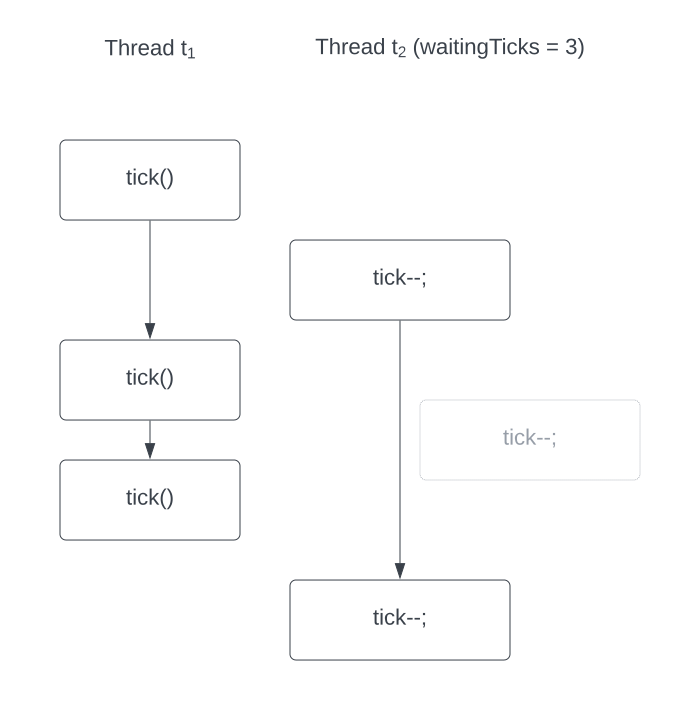
\includegraphics[scale=0.5]{chapters/Anhang/Klausuren/img/tick}
    \caption{Thread $t_1$ ruft 3 mal \texit{tick()} auf. Den Anforderungen nach müsste Thread $t_2$ danach aus der while-wait-Schleife herauskommen, erhält aber nicht die Sperre auf das Objekt von LogicalTime, um seinen eigenen Zähler rechtzeitig zu erniedrigen, bevor $t_1$ erneut \textit{tick()} aufruft. (Quelle: eigene)}
    \label{fig:tick}
\end{figure}

\section{Aufgabe 6}
Auch hier gilt, dass die Aufgabenstellung aufmerksam zu lesen ist.\\
Der Kreis soll erst ausgefüllt werden, wenn die Maustaste gelöst wird.

\begin{minted}[mathescape,
    linenos,
    numbersep=5pt,
    gobble=2,
    frame=lines,
    framesep=2mm]{java}
    private void mousePressed(double x, double y) {
        c = new Circle();
        c.setCenterX(x);
        c.setCenterY(y);
        c.setStroke(Color.RED);
        c.setFill(null); // oder Color.TRANSPARENT
        c.setRadius(RADIUS);
        graphicsPane.getChildren().add(c);
    }

    private void mouseReleased() {
        c.setFill(Color.RED);
        c = null;
    }
\end{minted}

\section{Aufgabe 8}

In der Abbildung \ref{fig:batchmodus} ist links der sequentielle Modus dargestellt, bei dem nach dem Senden einer Nachricht auf die Antwort des Servers gewartet wird, bevor eine neue Nachricht geschickt wird.
Dies wird i.d.R. verwendet, wenn das Senden einer neuen Nachricht abhängig ist von einem Ergebnis, die über die Server-Antwort übermittelt wird, oder wenn mit dem Server interagiert wird (Request abhängig vom Response).\\
Der Batch-Modus auf der rechten Seite der gleichen Abbildung ist schneller, da zwischen dem Senden von Nachrichten nicht auf Antworten gewartet werden müssen. \\
Erst nach dem Senden eine Batches von Nachrichten werden die dem Client zur Verfügung stehenden Antworten ausgelesen.\\

\noindent
In dieser Form des Batch-Modus besteht allerdings die Gefahr, dass es zu Verklemmungen kommt:
\begin{itemize}
    \item Bei dem Client kommen viele Nachrichten an, während er noch sendet.
    \item Die ankommenden Nachrichten für den Client werden gepuffert, bis sie ausgelesen werden (TCP- / OS-seitig).
    \item Läuft der Puffer voll, sorgt die Flusskontrolle (TCP) dafür, dass dem Sender mitgeteilt wird, dass keine Nachrichten mehr empfangen werden können, der Server sendet nicht mehr.
    \item Die zu sendenden Nachrichten des Servers werden in einen Puffer geschrieben.
    \item Der Sende-Puffer des Senders läuft voll.
    \item Bei dem nächsten Sende-Aufruf blockiert der Server, empfangene Nachrichten landen im Empfangspuffer
    \item Der Empfangspuffer des Servers läuft voll, der Client buffert die zu sendenden Nachrichten.
    \item Beide Anwendungen blockieren.
\end{itemize}

\\noindent
Um dieses Problem beim Batch-Modus zu umgehen, werden für das Senden und Empfangen zwei Threads auf Client-Seite erstellt: Ein Thread sendet, ein Thread empfängt. \\
Dadurch kann von dem Client immer wieder sein Empfangspuffer geleert werden, der Server wird beim Senden nicht blockiert.

\begin{figure}
    \centering
    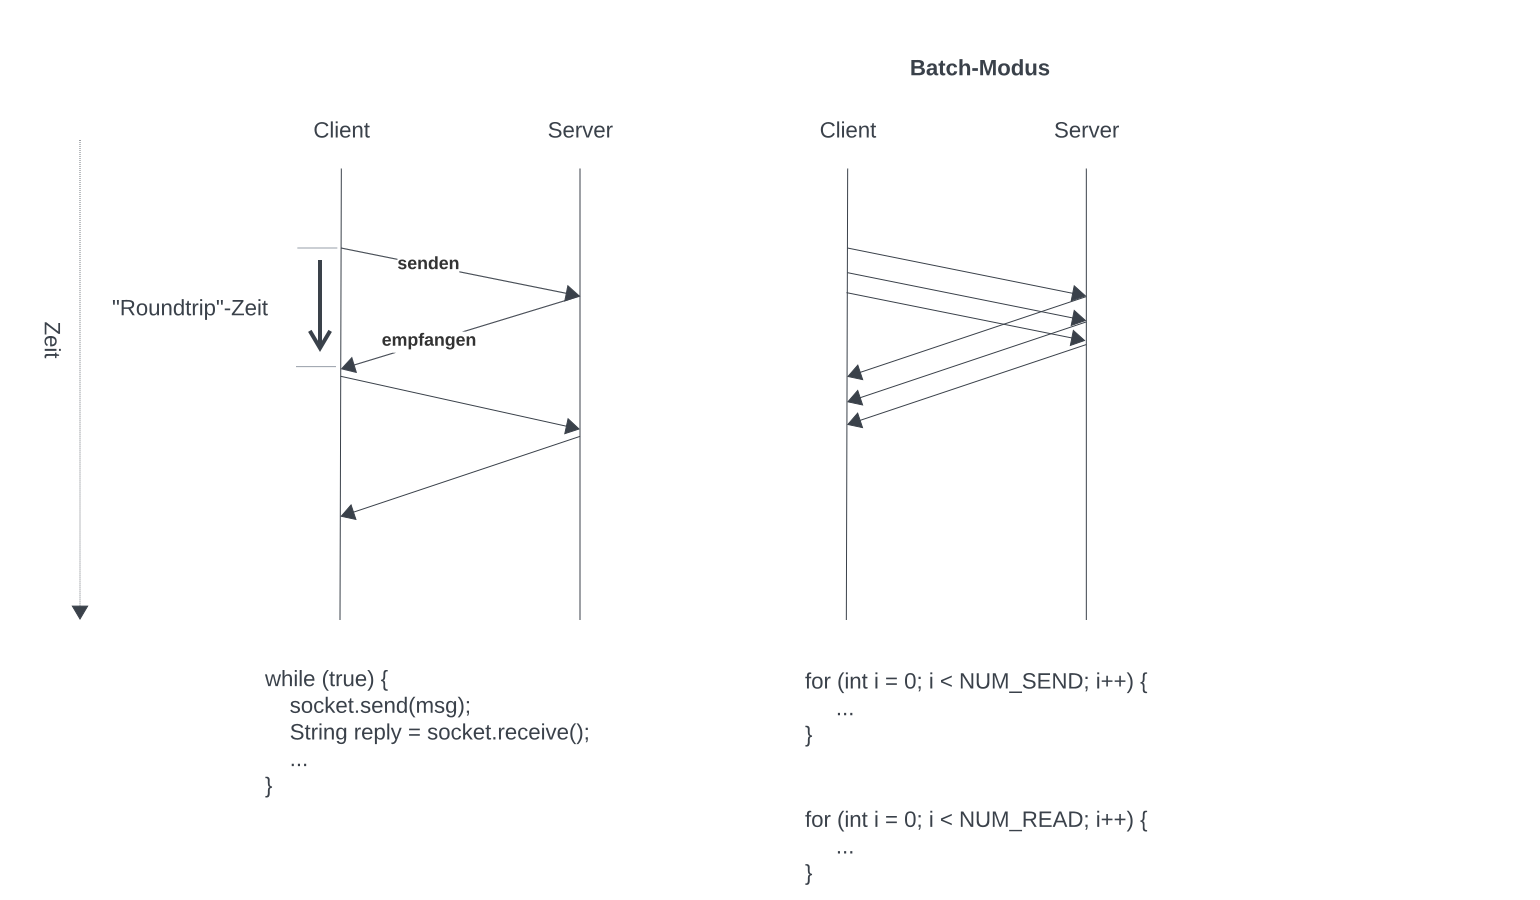
\includegraphics[scale=0.4]{chapters/Anhang/Klausuren/img/batchmodus}
    \caption{Vereinfachte Darstellung sequentieller Kommunikation und Batch-Modus (Quelle: eigene)}
    \label{fig:batchmodus}
\end{figure}
    
\begin{appendices}
    \input{chapters/Anhang/Zusatzaufgaben/index}
    \input{chapters/Anhang/Klausuren/ws13}
    \input{chapters/Anhang/Klausuren/ws15-16}
    \input{chapters/Anhang/Klausuren/ws16-17}
    \input{chapters/Anhang/Klausuren/ss19}
    \input{chapters/Anhang/Präsenzphase/index}

\end{appendices}


\end{appendices}

    \chapter{WS13}\label{ch:klausurws13}

\section{Aufgabe 1}
\subsection{Lösungsvorschlag}


\begin{minted}[mathescape,
    linenos,
    numbersep=5pt,
    gobble=2,
    fontsize=\small,
    frame=lines,
    framesep=2mm]{java}
    class Zahlenschloss {

        private int[] kombination;

        private int[] state;

        private boolean opened = false;

        public Zahlenschloss(int[] kombination) {
            this.kombination = kombination;
            this.state = new int[kombination.length];
        }

        public int anzahlRaedchen() {
            return kombination.length;
        }

        public synchronized int lesen(int radnummer) {
            return state[radnummer];
        }

        public synchronized void drehen(int radnummer, int zahl) {

            state[radnummer] = zahl;
            opened = true;
            for (int i = 0; i < anzahlRaedchen(); i++) {
                if (lesen(i) != kombination[i]) {
                    opened = false;
                    break;
                }
            }

            if (opened) {
                this.notify();
            }
        }

        public synchronized void warten() {

            while (!opened) {
                try {
                    this.wait();
                } catch (InterruptedException ignored) {}
            }
        }
    }
\end{minted}\\


\subsection{Anmerkung und Ergänzungen}

\begin{itemize}
    \item Es wird eine Wartebedingung benötigt, und zwar für die Methode \code{warten()}; ankommende Threads werden
    in die Warteschlange des Zahlenschloss-Objektes geschickt, wenn \code{opened} auf false gesetzt ist, ansonsten
    verlassen diese direkt die Methode wieder.\\
    Die Methode \code{drehen} benötigt keine separate Wartebedingung.
    Es reicht aus, sicherzustellen, dass das Zahlenschloss nicht gleichzeitig von anderen Threads benutzt werden kann:
    Die Methode \code{drehen} ist hierfür synchronisiert, damit das Zahlenschloss {insg.} immer nur eine Zustandsänderung
    erfährt - es sind andere Implementierungen möglich, in denen das Zahlenschloss dann von mehreren Threads gleichzeitig
    genutzt werden darf, wenn sich die Zugriffe anhand der ``Ziel``-\code{radnummer} unterscheiden, {bspw.} durch Mutex-Semaphore,
    die pro Radnummer verwendet werden\footnote{
        der gleichzeitige Zugriff auf unterschiedliche Arrays-Indizes ist erlaubt, s. `´17.4.1. Shared Variables``: \url{https://docs.oracle.com/javase/specs/jls/se21/html/jls-17.html#jls-1.4.1} - abgerufen 14.2.2024
    }.
    \item Es gibt nur eine Wartebedingung, von daher sollte \code{notify()} genügen.\\
    Wenn wir allerdings davon ausgehen, dass mehrere Threads über die Methode \code{warten()} in die Warteschlange des Objektes eingereiht worden sind,  sollte \code{notifyAll()} verwendet werden (siehe hierzu auch Abschnitt \ref{subsec:notifyAll}).
    Dennoch ist nicht garantiert, dass auch alle Threads aus der Warteschlange gelangen, denn es kann sein, dass ein anderer Thread die Methode \code{drehen()} betritt, dort die
    Zahlenkombination ändert und \code{opened} wieder auf \code{false} gesetzt wird. \\
    Ein anderer Thread, der nun in  \code{warten()} an die Reihe kommt, überprüft die Wartebedingung, und wird wieder in die Warteschlange eingereiht.
    Es ist also durchaus möglich, dass ein Thread nicht mehr aus der Methode \code{warten()} herauskommt.\\
    Dies könnte bspw. dadurch verhindert werden, dass die Threads in eine Queue gepackt werden, und in \code{drehen()} eine Wartebedingung eingefügt wird, die erst erfüllt ist,
    wenn die Queue geleert wurde oder aus ihr entnommen wurde, in der Reihenfolge, in der die Threads in die Queue eingereiht worden sind (\textit{FIFO}) (s. a. Abschnitt~\ref{subsec:readerwriterproblem}).
    \item Bei der Teilaufgabe mit der Schleife muss die komplette Schleife synchronisiert werden, was man durch ein \code{synchronized}-Statement erreicht\footnote{siehe Abschnitt~\ref{subsec:synchronizedstatement}.}
    \begin{minted}[mathescape,
        linenos,
        numbersep=5pt,
        gobble=2,
        fontsize=\small,
        frame=lines,
        framesep=2mm]{java}
        synchronized (zk) {
            for (int i = 0; i < anzahlRaedchen; i++) {
                System.out.println(zk.lesen(i));
            }
        }
    \end{minted}
    Ansonsten läuft man Gefahr, dass sich nach Auslesen der 1. Position der Wert von Position 2 geändert hat und dadurch eine
    Zahlenkombination ausgegeben wird, die es nicht gegeben hat:
    \begin{enumerate}
        \item $K\coloneqq[0, 0, 0]$
        \item Position $K_0$ wird ausgelesen und liefert $0$.
        \item Thread ändert $K_0$ zu $1$ $\implies K\coloneqq[1, 0, 0] $.
        \item Thread ändert $K_1$ zu $2$ $\implies K\coloneqq[1, 2, 0] $.
        \item Thread ändert $K_2$ zu $3$ $\implies K\coloneqq[1, 2, 3] $.
        \item Positionen $K_1$ und $K_2$ werden ausgelesen und liefern: $2, 3$
        \item Ausgabe: $0, 2, 3$ - diese Kombination hat es in dem Fall aber tatsächlich nicht gegeben.
    \end{enumerate}
\end{itemize}

\begin{tcolorbox}[colback=red!20,color=white,title=Anmerkung]
    Die Methode \code{lesen()} als \code{synchronized} zu markieren könnte man sich vlt. sparen, wenn man davon ausgeht,
    dass die Methode ohnehin in einem \code{synchronized}-Statement verwendet wird, um alle Rädchen abzulesen.\\
    Mehrere Threads können also nicht parallel auf unterschiedliche Positionen des Feldes zugreifen, wenn die Methode
    synchronisiert ist.\\
    Allerdings ist sowohl das Skript als auch das Buch recht klar, was in dieser Situation geschehen muss (s. Skript Fopt1/2, S. 9, außerdem \cite[31, Abschnitt 2.3.6]{Oec22}): Es muss (in diesem Kurs) immer \code{synchronized} verwendet werden, wenn gleichzeitig
    Daten geschrieben und gleichzeitig diese Daten gelesen werden sollen - und eine andere Implementierung, bei der die
    einzelnen Positionen ``gelocked`` sind, so dass ein gleichzeitiger Zugriff auf unterschiedliche Rädchen möglich ist, war nicht gefordert.\\
    Ggfl. würde in anderen Implementierungen der Einsatz von \code{AtomicReferenceArray}\footnote{s. \cite[157 ff.]{Oec22}
    s. ``Class AtomicReferenceArray<E>``: \url{https://docs.oracle.com/en/java/javase/21/docs/api/java.base/java/util/concurrent/atomic/AtomicReferenceArray.html} - abgerufen 15.2.2024
    } Sinn machen, aber das Lehrmaterial ist bereits sehr eindeutig bzgl. der Verwendung von \code{synchronized}.
\end{tcolorbox}



\section{Aufgabe 3}
\subsection{Lösungsvorschlag}

\subsection*{Statische Parallelität}
Statische Parallelität erlaubt es einem Server, eine \textit{fixe} Anzahl von Verbindungen gleichzeitig zu bedienen.\\
Hierbei wird ein Feld von Threads erstellt, wobei jeder Thread das \code{ServerSocket}-Objekt als Referenz übergeben bekommt.
In der \code{run()}-Methode wird dann über \code{accept()} in einer Endlosschleife auf eingehende Verbindungen gewartet, die dann so lange bedient werden, bis sich ein Client wieder abmeldet (oder eine andere Abbruchbedingung erfüllt ist, wie z.B. ein \code{SocketTimeout}).\\
Das sich ein Client abmeldet, bekommt man bspw. dadurch mit, dass \code{null} beim Lesen von einer Nachricht des Clients zurückgegeben wird (vgl. \cite[286]{Oec22}. \\
Siehe Abschnitt~\ref{sec:seqparserver} für ein Implementierungsbeispiel.



\subsection*{Dynamische Parallelität}

Bei der \textbf{Dynamischer Parallelität} erzeugt der Server für jede Verbindung einen neuen Thread, der so lange läuft, bis der Client die Verbindung wieder trennt.\\
Die Anzahl der Threads ändert sich dadurch laufend.\\
Wird die max. Anzahl erlaubter Threads nicht kontrolliert, kann es zu einer Überlastung des Server-Rechners kommen (bspw. durch einen Denial-of-Service-Angriff.)\\

\noindent
I.d.R. ist eine Mischform aus beidem geeignet, um mehrere Clients gleichzeitig bedienen zu können, und dabei nicht Gefahr zu laufen, durch dynamisches, unbegrenztes Wachstum der Anzahl der Threads überlastet zu werden.

    \chapter{WS13}\label{ch:klausurws5-16}

\section{Rechteck-Scroll (SS15 Aufgabe 2)}

Aufgabenstellung unklar.\\
Mögliche Implementierung unter \url{https://github.com/ThorstenSuckow/fopt/tree/main/src/main/java/klausurvorbereitung/foptws1516/MouseDragsSquareDemo}.

\section{Rechteck-Scroll (WS15/16 Aufgabe 1)}

Aufgabenstellung unklar.\\
Mögliche Implementierung unter \url{https://github.com/ThorstenSuckow/fopt/tree/main/src/main/java/klausurvorbereitung/foptws1516/MaxWeightDemo}.\\

\noindent
Es gibt nur eine Warteschlange für Threads in \code{use()}, es gibt keine Wartebedingung in \code{dontUse()} und damit auch keine weitere Warteschlange.\\
Es sind durch die Zugriffe auf unterschiedliche Indizes allerdings mehrere Wartebedingungen vorhanden, weshalb hab \code{notifyAll()} nutzen sollte,
sobald ein Zugriff auf ein Feld nach Aufruf von \code{dontUse} wieder möglich wird.\\
Ansonsten bestünde die Gefahr, dass bei dem Einsatz von \code{notify()} ein wartender Thread nicht geweckt wird, obwohl er weiterlaufen könnte:\\
Angenommen, das Feld $F$ hat eine Länge von $3$, das \code{maxWeight} ist mit $2$ konfiguriert.
Thread $t_1$ mit einer Laufzeit von $200\ sek$ bekommt Zugriff auf $F_0$, setzt $currentWeight$ auf $1$.\\
Thread $t_2$ mit einer Laufzeit von $1\ sek$ möchte auf $F_1$ zugreifen, setzt $currentWeight=2$ in die Warteschlange.\\
Thread $t_3$ meldet Zugriff auf $F_0$ an und gelangt in die Warteschlange.\\
Thread $t_4$ meldet Zugriff auf $F_1$ an und gelangt in die Warteschlange.\\
Thread $t_2$ ist mit der Bearbeitung von $F_1$ fertig, $currentWeight$ wird auf $1$ gesetzt, \code{notify()} wird aufgerufen.\\
Thread $t_3$ wird aus der Warteschlange geholt, kann aber nicht weiterarbeiten, da $F_0$ noch durch den länger dauernden $t_1$ blockiert ist, und kommt wieder in die Warteschlange.\\

\noindent
Offensichtlich hätte in dem Beispiel \code{notifyAll()} dazu geführt, dass auch $T_4$ seine Wartebedingung hätte überprüfen können, und hätte so Zugriff auf $F_1$ bekommen.
Stattdessen muss nun gewartet werden, bis das nächste \code{notify()} aufgerufen wird, oder ein neu ankommender Thread $F_1$ belegt.

    \chapter{WS16-17}\label{ch:klausurws16-17}

\section{Aufgabe 1}
\subsection{Lösungshinweis}

Die erste Aufgabe verdeutlicht, was bei einem \code{notifyAll()} und unsauber gesetzten Wartebedingungen passieren kann.\\
Sei folgender Quellcode gegeben:


\begin{minted}[mathescape,
    linenos,
    numbersep=5pt,
    gobble=2,
    fontsize=\small,
    frame=lines,
    framesep=2mm]{java}
    class Cond1AndCond2 {

        private boolean cond1;
        private boolean cond2;

        public synchronized void setCond1(boolean c) {
            cond1 = c;
            notifyAll();
        }

        public synchronized void setCond2(boolean c) {
            cond2 = c;
            notifyAll();
        }

        public synchronized void cond1AndCond2() {
            while(!cond1) {
                try {
                    wait();
                } catch(InterruptedException e) { }
            }

            while(!cond2) {
                try {
                    wait();
                } catch(InterruptedException e) {}
            }
            System.out.println("cond1 and cond2:" + cond1 + " " + cond2);
        }
    }
\end{minted}\\

Man sollte auf den ersten Blick meinen, dass \code{cond1} und \code{cond2} beide \code{true} sein müssen, damit die Ausgabe erfolgt.\\
Tatsächlich ist es aber so, dass es in der Methode zwei unterschiedliche Wartebedingungen gibt.\\
Die erste Wartebedingung schickt einen Thread in die Warteschlange, wenn \code{cond1 == false} gilt.\\
Setzt ein anderer Thread über \code{setCond1(true)} das Attribut entsprechend auf \code{true}, bewirkt der nachfolgende Aufruf von \code{notifyAll()}, dass alle \textit{wartenden} Threads aus der Warteschlange entfernt werden und erneut um eine Sperre des Objektes konkurrieren.\\
Erhält ein entsprechender Thread $t_w$ die Sperre auf das Objekt und kann seine \textit{while-wait-Schleife} verlassen, kann es vorkommen, dass er erneut in die Warteschlange eingereiht wird, wegen der nachfolgenden Wartebedingung \code{cond2 == false}.\\
Angenommen, ein weiterer Thread ruft nun \code{setCond2(true)} auf, und $t_w$ kommt aus der Warteschlange und konkurriert erneut und um die Sperre des Objektes, dann kann es vorkommen, das ein anderer Thread zunächst die Sperre erhält, \code{cond1} wieder auf \code{false} setzt, dann erhält $t_w$ die Sperre, überprüft die Wartebedingung \code{cond2 == false}.\\
Wegen \code{cond2} gelangt er aus der \textit{while-wait-Schleife} und die Ausgabe erfolgt - da zwischenzeitlich \code{cond1} wieder auf \code{false} gesetzt wurde, ist die erwartete Ausgabe nicht \code{true true}, sondern \code{false true} (s. Abbildung \ref{fig:cond1cond2}).\\

\begin{figure}
    \centering
    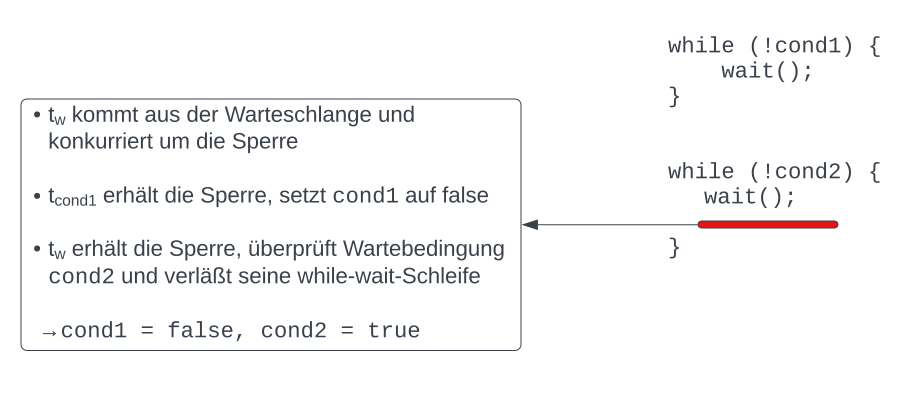
\includegraphics[scale=0.4]{chapters/Anhang/Klausuren/img/cond1cond2}
    \caption{in den rot markierten Bereich konkurriert $t_w$ um die Sperre des Objektes - wenn durch einen anderen Thread, der vor $t_w$ die Sperre erhält, \textit{cond1} auf \textit{false} gesetzt wird, stimmt die Ausgabe nicht mit der erwarteten überein. (Quelle: eigene)}
    \label{fig:cond1cond2}
\end{figure}

\noindent
Die korrekte Wartebedingung sollte lauten:

\begin{minted}[mathescape,
    linenos,
    numbersep=5pt,
    gobble=2,
    fontsize=\small,
    frame=lines,
    framesep=2mm]{java}
    public synchronized void cond1AndCond2() {
        while(!cond1 || !cond2) {
            try {
                wait();
            } catch(InterruptedException e) { }
        }
        System.out.println("cond1 and cond2:" + cond1 + " " + cond2);
    }
\end{minted}\\

Darüber hinaus müßte \code{notifyAll()} nur aufgerufen werden, wenn sowohl \code{cond1} als auch \code{cond2} auf \code{true} gesetzt sind, was leicht in den entsprechenden Methoden überprüft werden kann.
    \chapter{SS19}\label{ch:klausurss19}

\section{Aufgabe 1}

Bei der Aufgabe ist es wichtig, die Anforderungen genau zu beachten.\\
Ob eine Thread die while-wait-Schleife verlassen darf, wird von der Methode \code{tick()} gesteuert - wieviele Ticks ein Thread in der Schleife bleiben soll, wird von dem jeweiligen Thread definiert.\\
Die \code{tick()}-Methode wird von anderen Threads aufgerufen, es kann also durchaus vorkommen, dass mehrmals hintereinander
die \code{notifyAll()}-Methode aufgerufen wird - diese entfernt alle Threads aus der Warteschlange, damit die Threads ihre
Wartebedingungen erneut überprüfen können.\\
da \code{tick()} aber auch gleichzeitig einen Zähler realisieren soll, \textit{muss} es in der Methode auch eine Zählvariable geben, anhand derer die in der while-wait-Schleife enthaltenen Threads feststellen können, wie oft \code{tick()} aufgerufen wurde, um entsprechend aus der Schleife und nachfolgend der Methode herauszukommen.

\begin{figure}
    \centering
    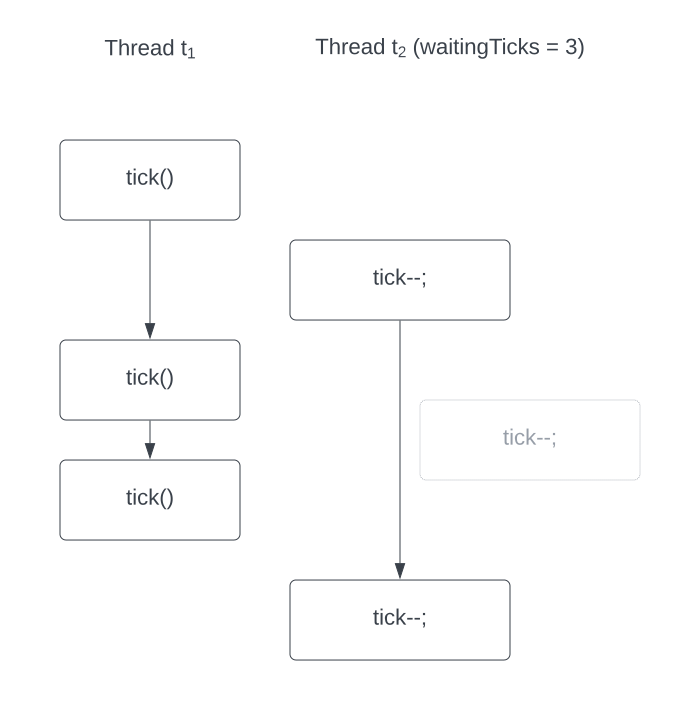
\includegraphics[scale=0.5]{chapters/Anhang/Klausuren/img/tick}
    \caption{Thread $t_1$ ruft 3 mal \texit{tick()} auf. Den Anforderungen nach müsste Thread $t_2$ danach aus der while-wait-Schleife herauskommen, erhält aber nicht die Sperre auf das Objekt von LogicalTime, um seinen eigenen Zähler rechtzeitig zu erniedrigen, bevor $t_1$ erneut \textit{tick()} aufruft. (Quelle: eigene)}
    \label{fig:tick}
\end{figure}

\section{Aufgabe 6}
Auch hier gilt, dass die Aufgabenstellung aufmerksam zu lesen ist.\\
Der Kreis soll erst ausgefüllt werden, wenn die Maustaste gelöst wird.

\begin{minted}[mathescape,
    linenos,
    numbersep=5pt,
    gobble=2,
    frame=lines,
    framesep=2mm]{java}
    private void mousePressed(double x, double y) {
        c = new Circle();
        c.setCenterX(x);
        c.setCenterY(y);
        c.setStroke(Color.RED);
        c.setFill(null); // oder Color.TRANSPARENT
        c.setRadius(RADIUS);
        graphicsPane.getChildren().add(c);
    }

    private void mouseReleased() {
        c.setFill(Color.RED);
        c = null;
    }
\end{minted}

\section{Aufgabe 8}

In der Abbildung \ref{fig:batchmodus} ist links der sequentielle Modus dargestellt, bei dem nach dem Senden einer Nachricht auf die Antwort des Servers gewartet wird, bevor eine neue Nachricht geschickt wird.
Dies wird i.d.R. verwendet, wenn das Senden einer neuen Nachricht abhängig ist von einem Ergebnis, die über die Server-Antwort übermittelt wird, oder wenn mit dem Server interagiert wird (Request abhängig vom Response).\\
Der Batch-Modus auf der rechten Seite der gleichen Abbildung ist schneller, da zwischen dem Senden von Nachrichten nicht auf Antworten gewartet werden müssen. \\
Erst nach dem Senden eine Batches von Nachrichten werden die dem Client zur Verfügung stehenden Antworten ausgelesen.\\

\noindent
In dieser Form des Batch-Modus besteht allerdings die Gefahr, dass es zu Verklemmungen kommt:
\begin{itemize}
    \item Bei dem Client kommen viele Nachrichten an, während er noch sendet.
    \item Die ankommenden Nachrichten für den Client werden gepuffert, bis sie ausgelesen werden (TCP- / OS-seitig).
    \item Läuft der Puffer voll, sorgt die Flusskontrolle (TCP) dafür, dass dem Sender mitgeteilt wird, dass keine Nachrichten mehr empfangen werden können, der Server sendet nicht mehr.
    \item Die zu sendenden Nachrichten des Servers werden in einen Puffer geschrieben.
    \item Der Sende-Puffer des Senders läuft voll.
    \item Bei dem nächsten Sende-Aufruf blockiert der Server, empfangene Nachrichten landen im Empfangspuffer
    \item Der Empfangspuffer des Servers läuft voll, der Client buffert die zu sendenden Nachrichten.
    \item Beide Anwendungen blockieren.
\end{itemize}

\\noindent
Um dieses Problem beim Batch-Modus zu umgehen, werden für das Senden und Empfangen zwei Threads auf Client-Seite erstellt: Ein Thread sendet, ein Thread empfängt. \\
Dadurch kann von dem Client immer wieder sein Empfangspuffer geleert werden, der Server wird beim Senden nicht blockiert.

\begin{figure}
    \centering
    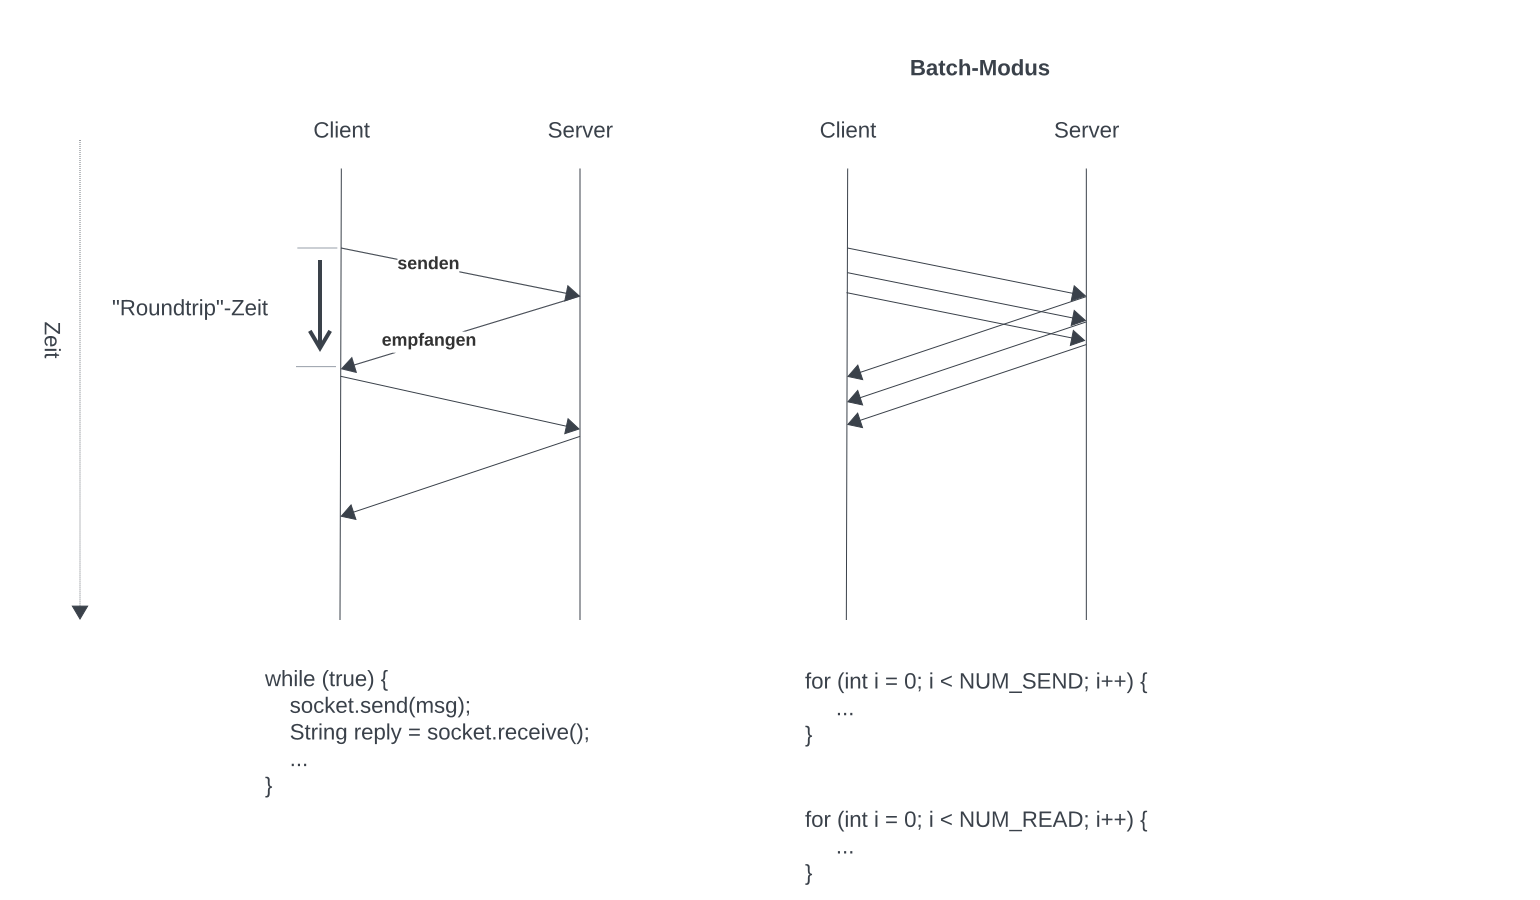
\includegraphics[scale=0.4]{chapters/Anhang/Klausuren/img/batchmodus}
    \caption{Vereinfachte Darstellung sequentieller Kommunikation und Batch-Modus (Quelle: eigene)}
    \label{fig:batchmodus}
\end{figure}
    
\begin{appendices}
    
\begin{appendices}
    \input{chapters/Anhang/Zusatzaufgaben/index}
    \input{chapters/Anhang/Klausuren/ws13}
    \input{chapters/Anhang/Klausuren/ws15-16}
    \input{chapters/Anhang/Klausuren/ws16-17}
    \input{chapters/Anhang/Klausuren/ss19}
    \input{chapters/Anhang/Präsenzphase/index}

\end{appendices}

    \chapter{WS13}\label{ch:klausurws13}

\section{Aufgabe 1}
\subsection{Lösungsvorschlag}


\begin{minted}[mathescape,
    linenos,
    numbersep=5pt,
    gobble=2,
    fontsize=\small,
    frame=lines,
    framesep=2mm]{java}
    class Zahlenschloss {

        private int[] kombination;

        private int[] state;

        private boolean opened = false;

        public Zahlenschloss(int[] kombination) {
            this.kombination = kombination;
            this.state = new int[kombination.length];
        }

        public int anzahlRaedchen() {
            return kombination.length;
        }

        public synchronized int lesen(int radnummer) {
            return state[radnummer];
        }

        public synchronized void drehen(int radnummer, int zahl) {

            state[radnummer] = zahl;
            opened = true;
            for (int i = 0; i < anzahlRaedchen(); i++) {
                if (lesen(i) != kombination[i]) {
                    opened = false;
                    break;
                }
            }

            if (opened) {
                this.notify();
            }
        }

        public synchronized void warten() {

            while (!opened) {
                try {
                    this.wait();
                } catch (InterruptedException ignored) {}
            }
        }
    }
\end{minted}\\


\subsection{Anmerkung und Ergänzungen}

\begin{itemize}
    \item Es wird eine Wartebedingung benötigt, und zwar für die Methode \code{warten()}; ankommende Threads werden
    in die Warteschlange des Zahlenschloss-Objektes geschickt, wenn \code{opened} auf false gesetzt ist, ansonsten
    verlassen diese direkt die Methode wieder.\\
    Die Methode \code{drehen} benötigt keine separate Wartebedingung.
    Es reicht aus, sicherzustellen, dass das Zahlenschloss nicht gleichzeitig von anderen Threads benutzt werden kann:
    Die Methode \code{drehen} ist hierfür synchronisiert, damit das Zahlenschloss {insg.} immer nur eine Zustandsänderung
    erfährt - es sind andere Implementierungen möglich, in denen das Zahlenschloss dann von mehreren Threads gleichzeitig
    genutzt werden darf, wenn sich die Zugriffe anhand der ``Ziel``-\code{radnummer} unterscheiden, {bspw.} durch Mutex-Semaphore,
    die pro Radnummer verwendet werden\footnote{
        der gleichzeitige Zugriff auf unterschiedliche Arrays-Indizes ist erlaubt, s. `´17.4.1. Shared Variables``: \url{https://docs.oracle.com/javase/specs/jls/se21/html/jls-17.html#jls-1.4.1} - abgerufen 14.2.2024
    }.
    \item Es gibt nur eine Wartebedingung, von daher sollte \code{notify()} genügen.\\
    Wenn wir allerdings davon ausgehen, dass mehrere Threads über die Methode \code{warten()} in die Warteschlange des Objektes eingereiht worden sind,  sollte \code{notifyAll()} verwendet werden (siehe hierzu auch Abschnitt \ref{subsec:notifyAll}).
    Dennoch ist nicht garantiert, dass auch alle Threads aus der Warteschlange gelangen, denn es kann sein, dass ein anderer Thread die Methode \code{drehen()} betritt, dort die
    Zahlenkombination ändert und \code{opened} wieder auf \code{false} gesetzt wird. \\
    Ein anderer Thread, der nun in  \code{warten()} an die Reihe kommt, überprüft die Wartebedingung, und wird wieder in die Warteschlange eingereiht.
    Es ist also durchaus möglich, dass ein Thread nicht mehr aus der Methode \code{warten()} herauskommt.\\
    Dies könnte bspw. dadurch verhindert werden, dass die Threads in eine Queue gepackt werden, und in \code{drehen()} eine Wartebedingung eingefügt wird, die erst erfüllt ist,
    wenn die Queue geleert wurde oder aus ihr entnommen wurde, in der Reihenfolge, in der die Threads in die Queue eingereiht worden sind (\textit{FIFO}) (s. a. Abschnitt~\ref{subsec:readerwriterproblem}).
    \item Bei der Teilaufgabe mit der Schleife muss die komplette Schleife synchronisiert werden, was man durch ein \code{synchronized}-Statement erreicht\footnote{siehe Abschnitt~\ref{subsec:synchronizedstatement}.}
    \begin{minted}[mathescape,
        linenos,
        numbersep=5pt,
        gobble=2,
        fontsize=\small,
        frame=lines,
        framesep=2mm]{java}
        synchronized (zk) {
            for (int i = 0; i < anzahlRaedchen; i++) {
                System.out.println(zk.lesen(i));
            }
        }
    \end{minted}
    Ansonsten läuft man Gefahr, dass sich nach Auslesen der 1. Position der Wert von Position 2 geändert hat und dadurch eine
    Zahlenkombination ausgegeben wird, die es nicht gegeben hat:
    \begin{enumerate}
        \item $K\coloneqq[0, 0, 0]$
        \item Position $K_0$ wird ausgelesen und liefert $0$.
        \item Thread ändert $K_0$ zu $1$ $\implies K\coloneqq[1, 0, 0] $.
        \item Thread ändert $K_1$ zu $2$ $\implies K\coloneqq[1, 2, 0] $.
        \item Thread ändert $K_2$ zu $3$ $\implies K\coloneqq[1, 2, 3] $.
        \item Positionen $K_1$ und $K_2$ werden ausgelesen und liefern: $2, 3$
        \item Ausgabe: $0, 2, 3$ - diese Kombination hat es in dem Fall aber tatsächlich nicht gegeben.
    \end{enumerate}
\end{itemize}

\begin{tcolorbox}[colback=red!20,color=white,title=Anmerkung]
    Die Methode \code{lesen()} als \code{synchronized} zu markieren könnte man sich vlt. sparen, wenn man davon ausgeht,
    dass die Methode ohnehin in einem \code{synchronized}-Statement verwendet wird, um alle Rädchen abzulesen.\\
    Mehrere Threads können also nicht parallel auf unterschiedliche Positionen des Feldes zugreifen, wenn die Methode
    synchronisiert ist.\\
    Allerdings ist sowohl das Skript als auch das Buch recht klar, was in dieser Situation geschehen muss (s. Skript Fopt1/2, S. 9, außerdem \cite[31, Abschnitt 2.3.6]{Oec22}): Es muss (in diesem Kurs) immer \code{synchronized} verwendet werden, wenn gleichzeitig
    Daten geschrieben und gleichzeitig diese Daten gelesen werden sollen - und eine andere Implementierung, bei der die
    einzelnen Positionen ``gelocked`` sind, so dass ein gleichzeitiger Zugriff auf unterschiedliche Rädchen möglich ist, war nicht gefordert.\\
    Ggfl. würde in anderen Implementierungen der Einsatz von \code{AtomicReferenceArray}\footnote{s. \cite[157 ff.]{Oec22}
    s. ``Class AtomicReferenceArray<E>``: \url{https://docs.oracle.com/en/java/javase/21/docs/api/java.base/java/util/concurrent/atomic/AtomicReferenceArray.html} - abgerufen 15.2.2024
    } Sinn machen, aber das Lehrmaterial ist bereits sehr eindeutig bzgl. der Verwendung von \code{synchronized}.
\end{tcolorbox}



\section{Aufgabe 3}
\subsection{Lösungsvorschlag}

\subsection*{Statische Parallelität}
Statische Parallelität erlaubt es einem Server, eine \textit{fixe} Anzahl von Verbindungen gleichzeitig zu bedienen.\\
Hierbei wird ein Feld von Threads erstellt, wobei jeder Thread das \code{ServerSocket}-Objekt als Referenz übergeben bekommt.
In der \code{run()}-Methode wird dann über \code{accept()} in einer Endlosschleife auf eingehende Verbindungen gewartet, die dann so lange bedient werden, bis sich ein Client wieder abmeldet (oder eine andere Abbruchbedingung erfüllt ist, wie z.B. ein \code{SocketTimeout}).\\
Das sich ein Client abmeldet, bekommt man bspw. dadurch mit, dass \code{null} beim Lesen von einer Nachricht des Clients zurückgegeben wird (vgl. \cite[286]{Oec22}. \\
Siehe Abschnitt~\ref{sec:seqparserver} für ein Implementierungsbeispiel.



\subsection*{Dynamische Parallelität}

Bei der \textbf{Dynamischer Parallelität} erzeugt der Server für jede Verbindung einen neuen Thread, der so lange läuft, bis der Client die Verbindung wieder trennt.\\
Die Anzahl der Threads ändert sich dadurch laufend.\\
Wird die max. Anzahl erlaubter Threads nicht kontrolliert, kann es zu einer Überlastung des Server-Rechners kommen (bspw. durch einen Denial-of-Service-Angriff.)\\

\noindent
I.d.R. ist eine Mischform aus beidem geeignet, um mehrere Clients gleichzeitig bedienen zu können, und dabei nicht Gefahr zu laufen, durch dynamisches, unbegrenztes Wachstum der Anzahl der Threads überlastet zu werden.

    \chapter{WS13}\label{ch:klausurws5-16}

\section{Rechteck-Scroll (SS15 Aufgabe 2)}

Aufgabenstellung unklar.\\
Mögliche Implementierung unter \url{https://github.com/ThorstenSuckow/fopt/tree/main/src/main/java/klausurvorbereitung/foptws1516/MouseDragsSquareDemo}.

\section{Rechteck-Scroll (WS15/16 Aufgabe 1)}

Aufgabenstellung unklar.\\
Mögliche Implementierung unter \url{https://github.com/ThorstenSuckow/fopt/tree/main/src/main/java/klausurvorbereitung/foptws1516/MaxWeightDemo}.\\

\noindent
Es gibt nur eine Warteschlange für Threads in \code{use()}, es gibt keine Wartebedingung in \code{dontUse()} und damit auch keine weitere Warteschlange.\\
Es sind durch die Zugriffe auf unterschiedliche Indizes allerdings mehrere Wartebedingungen vorhanden, weshalb hab \code{notifyAll()} nutzen sollte,
sobald ein Zugriff auf ein Feld nach Aufruf von \code{dontUse} wieder möglich wird.\\
Ansonsten bestünde die Gefahr, dass bei dem Einsatz von \code{notify()} ein wartender Thread nicht geweckt wird, obwohl er weiterlaufen könnte:\\
Angenommen, das Feld $F$ hat eine Länge von $3$, das \code{maxWeight} ist mit $2$ konfiguriert.
Thread $t_1$ mit einer Laufzeit von $200\ sek$ bekommt Zugriff auf $F_0$, setzt $currentWeight$ auf $1$.\\
Thread $t_2$ mit einer Laufzeit von $1\ sek$ möchte auf $F_1$ zugreifen, setzt $currentWeight=2$ in die Warteschlange.\\
Thread $t_3$ meldet Zugriff auf $F_0$ an und gelangt in die Warteschlange.\\
Thread $t_4$ meldet Zugriff auf $F_1$ an und gelangt in die Warteschlange.\\
Thread $t_2$ ist mit der Bearbeitung von $F_1$ fertig, $currentWeight$ wird auf $1$ gesetzt, \code{notify()} wird aufgerufen.\\
Thread $t_3$ wird aus der Warteschlange geholt, kann aber nicht weiterarbeiten, da $F_0$ noch durch den länger dauernden $t_1$ blockiert ist, und kommt wieder in die Warteschlange.\\

\noindent
Offensichtlich hätte in dem Beispiel \code{notifyAll()} dazu geführt, dass auch $T_4$ seine Wartebedingung hätte überprüfen können, und hätte so Zugriff auf $F_1$ bekommen.
Stattdessen muss nun gewartet werden, bis das nächste \code{notify()} aufgerufen wird, oder ein neu ankommender Thread $F_1$ belegt.

    \chapter{WS16-17}\label{ch:klausurws16-17}

\section{Aufgabe 1}
\subsection{Lösungshinweis}

Die erste Aufgabe verdeutlicht, was bei einem \code{notifyAll()} und unsauber gesetzten Wartebedingungen passieren kann.\\
Sei folgender Quellcode gegeben:


\begin{minted}[mathescape,
    linenos,
    numbersep=5pt,
    gobble=2,
    fontsize=\small,
    frame=lines,
    framesep=2mm]{java}
    class Cond1AndCond2 {

        private boolean cond1;
        private boolean cond2;

        public synchronized void setCond1(boolean c) {
            cond1 = c;
            notifyAll();
        }

        public synchronized void setCond2(boolean c) {
            cond2 = c;
            notifyAll();
        }

        public synchronized void cond1AndCond2() {
            while(!cond1) {
                try {
                    wait();
                } catch(InterruptedException e) { }
            }

            while(!cond2) {
                try {
                    wait();
                } catch(InterruptedException e) {}
            }
            System.out.println("cond1 and cond2:" + cond1 + " " + cond2);
        }
    }
\end{minted}\\

Man sollte auf den ersten Blick meinen, dass \code{cond1} und \code{cond2} beide \code{true} sein müssen, damit die Ausgabe erfolgt.\\
Tatsächlich ist es aber so, dass es in der Methode zwei unterschiedliche Wartebedingungen gibt.\\
Die erste Wartebedingung schickt einen Thread in die Warteschlange, wenn \code{cond1 == false} gilt.\\
Setzt ein anderer Thread über \code{setCond1(true)} das Attribut entsprechend auf \code{true}, bewirkt der nachfolgende Aufruf von \code{notifyAll()}, dass alle \textit{wartenden} Threads aus der Warteschlange entfernt werden und erneut um eine Sperre des Objektes konkurrieren.\\
Erhält ein entsprechender Thread $t_w$ die Sperre auf das Objekt und kann seine \textit{while-wait-Schleife} verlassen, kann es vorkommen, dass er erneut in die Warteschlange eingereiht wird, wegen der nachfolgenden Wartebedingung \code{cond2 == false}.\\
Angenommen, ein weiterer Thread ruft nun \code{setCond2(true)} auf, und $t_w$ kommt aus der Warteschlange und konkurriert erneut und um die Sperre des Objektes, dann kann es vorkommen, das ein anderer Thread zunächst die Sperre erhält, \code{cond1} wieder auf \code{false} setzt, dann erhält $t_w$ die Sperre, überprüft die Wartebedingung \code{cond2 == false}.\\
Wegen \code{cond2} gelangt er aus der \textit{while-wait-Schleife} und die Ausgabe erfolgt - da zwischenzeitlich \code{cond1} wieder auf \code{false} gesetzt wurde, ist die erwartete Ausgabe nicht \code{true true}, sondern \code{false true} (s. Abbildung \ref{fig:cond1cond2}).\\

\begin{figure}
    \centering
    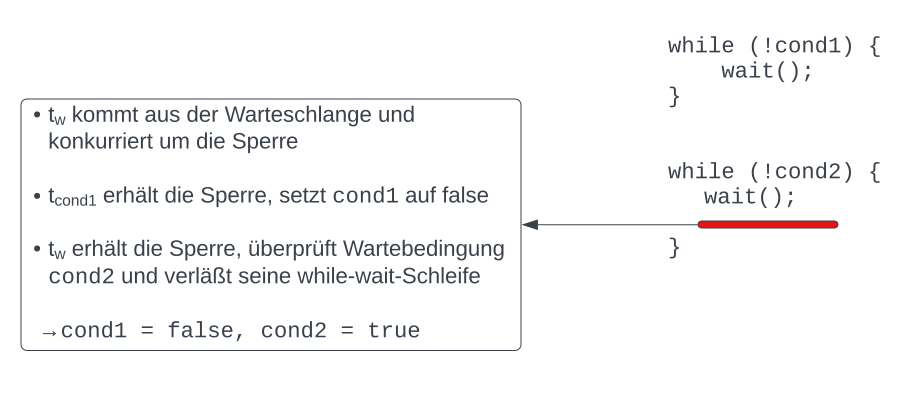
\includegraphics[scale=0.4]{chapters/Anhang/Klausuren/img/cond1cond2}
    \caption{in den rot markierten Bereich konkurriert $t_w$ um die Sperre des Objektes - wenn durch einen anderen Thread, der vor $t_w$ die Sperre erhält, \textit{cond1} auf \textit{false} gesetzt wird, stimmt die Ausgabe nicht mit der erwarteten überein. (Quelle: eigene)}
    \label{fig:cond1cond2}
\end{figure}

\noindent
Die korrekte Wartebedingung sollte lauten:

\begin{minted}[mathescape,
    linenos,
    numbersep=5pt,
    gobble=2,
    fontsize=\small,
    frame=lines,
    framesep=2mm]{java}
    public synchronized void cond1AndCond2() {
        while(!cond1 || !cond2) {
            try {
                wait();
            } catch(InterruptedException e) { }
        }
        System.out.println("cond1 and cond2:" + cond1 + " " + cond2);
    }
\end{minted}\\

Darüber hinaus müßte \code{notifyAll()} nur aufgerufen werden, wenn sowohl \code{cond1} als auch \code{cond2} auf \code{true} gesetzt sind, was leicht in den entsprechenden Methoden überprüft werden kann.
    \chapter{SS19}\label{ch:klausurss19}

\section{Aufgabe 1}

Bei der Aufgabe ist es wichtig, die Anforderungen genau zu beachten.\\
Ob eine Thread die while-wait-Schleife verlassen darf, wird von der Methode \code{tick()} gesteuert - wieviele Ticks ein Thread in der Schleife bleiben soll, wird von dem jeweiligen Thread definiert.\\
Die \code{tick()}-Methode wird von anderen Threads aufgerufen, es kann also durchaus vorkommen, dass mehrmals hintereinander
die \code{notifyAll()}-Methode aufgerufen wird - diese entfernt alle Threads aus der Warteschlange, damit die Threads ihre
Wartebedingungen erneut überprüfen können.\\
da \code{tick()} aber auch gleichzeitig einen Zähler realisieren soll, \textit{muss} es in der Methode auch eine Zählvariable geben, anhand derer die in der while-wait-Schleife enthaltenen Threads feststellen können, wie oft \code{tick()} aufgerufen wurde, um entsprechend aus der Schleife und nachfolgend der Methode herauszukommen.

\begin{figure}
    \centering
    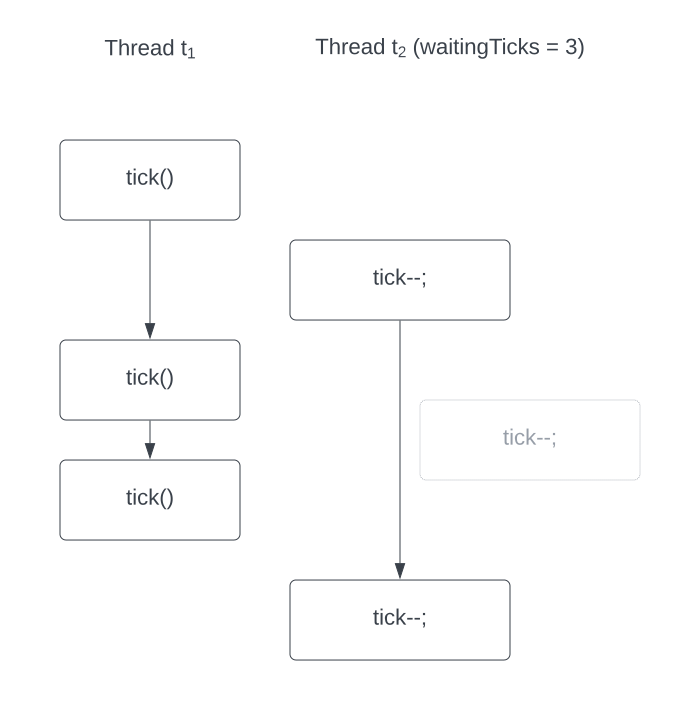
\includegraphics[scale=0.5]{chapters/Anhang/Klausuren/img/tick}
    \caption{Thread $t_1$ ruft 3 mal \texit{tick()} auf. Den Anforderungen nach müsste Thread $t_2$ danach aus der while-wait-Schleife herauskommen, erhält aber nicht die Sperre auf das Objekt von LogicalTime, um seinen eigenen Zähler rechtzeitig zu erniedrigen, bevor $t_1$ erneut \textit{tick()} aufruft. (Quelle: eigene)}
    \label{fig:tick}
\end{figure}

\section{Aufgabe 6}
Auch hier gilt, dass die Aufgabenstellung aufmerksam zu lesen ist.\\
Der Kreis soll erst ausgefüllt werden, wenn die Maustaste gelöst wird.

\begin{minted}[mathescape,
    linenos,
    numbersep=5pt,
    gobble=2,
    frame=lines,
    framesep=2mm]{java}
    private void mousePressed(double x, double y) {
        c = new Circle();
        c.setCenterX(x);
        c.setCenterY(y);
        c.setStroke(Color.RED);
        c.setFill(null); // oder Color.TRANSPARENT
        c.setRadius(RADIUS);
        graphicsPane.getChildren().add(c);
    }

    private void mouseReleased() {
        c.setFill(Color.RED);
        c = null;
    }
\end{minted}

\section{Aufgabe 8}

In der Abbildung \ref{fig:batchmodus} ist links der sequentielle Modus dargestellt, bei dem nach dem Senden einer Nachricht auf die Antwort des Servers gewartet wird, bevor eine neue Nachricht geschickt wird.
Dies wird i.d.R. verwendet, wenn das Senden einer neuen Nachricht abhängig ist von einem Ergebnis, die über die Server-Antwort übermittelt wird, oder wenn mit dem Server interagiert wird (Request abhängig vom Response).\\
Der Batch-Modus auf der rechten Seite der gleichen Abbildung ist schneller, da zwischen dem Senden von Nachrichten nicht auf Antworten gewartet werden müssen. \\
Erst nach dem Senden eine Batches von Nachrichten werden die dem Client zur Verfügung stehenden Antworten ausgelesen.\\

\noindent
In dieser Form des Batch-Modus besteht allerdings die Gefahr, dass es zu Verklemmungen kommt:
\begin{itemize}
    \item Bei dem Client kommen viele Nachrichten an, während er noch sendet.
    \item Die ankommenden Nachrichten für den Client werden gepuffert, bis sie ausgelesen werden (TCP- / OS-seitig).
    \item Läuft der Puffer voll, sorgt die Flusskontrolle (TCP) dafür, dass dem Sender mitgeteilt wird, dass keine Nachrichten mehr empfangen werden können, der Server sendet nicht mehr.
    \item Die zu sendenden Nachrichten des Servers werden in einen Puffer geschrieben.
    \item Der Sende-Puffer des Senders läuft voll.
    \item Bei dem nächsten Sende-Aufruf blockiert der Server, empfangene Nachrichten landen im Empfangspuffer
    \item Der Empfangspuffer des Servers läuft voll, der Client buffert die zu sendenden Nachrichten.
    \item Beide Anwendungen blockieren.
\end{itemize}

\\noindent
Um dieses Problem beim Batch-Modus zu umgehen, werden für das Senden und Empfangen zwei Threads auf Client-Seite erstellt: Ein Thread sendet, ein Thread empfängt. \\
Dadurch kann von dem Client immer wieder sein Empfangspuffer geleert werden, der Server wird beim Senden nicht blockiert.

\begin{figure}
    \centering
    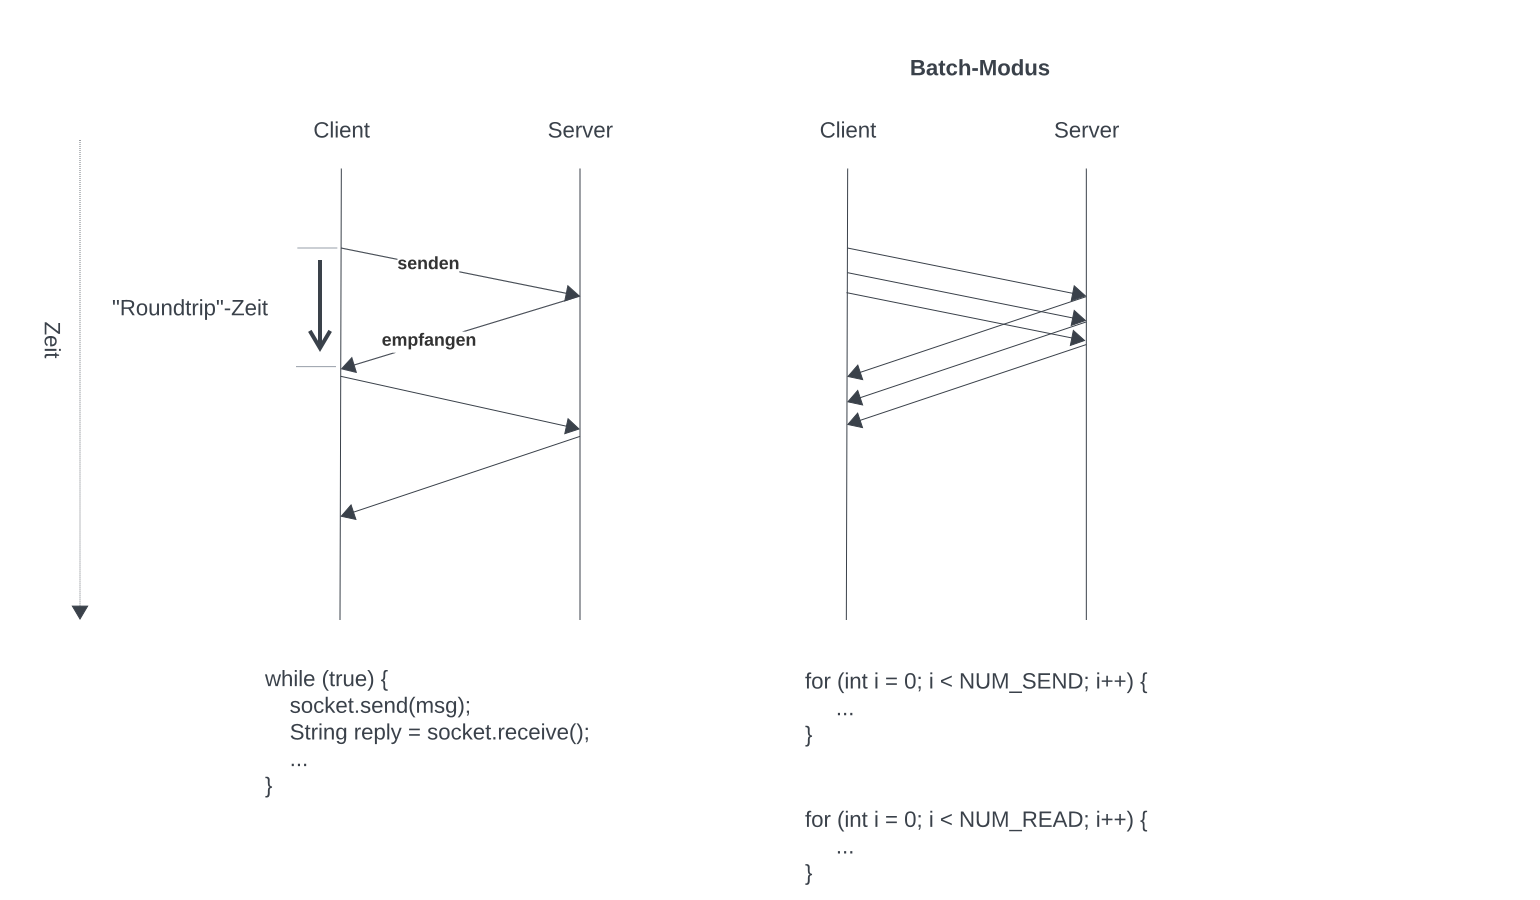
\includegraphics[scale=0.4]{chapters/Anhang/Klausuren/img/batchmodus}
    \caption{Vereinfachte Darstellung sequentieller Kommunikation und Batch-Modus (Quelle: eigene)}
    \label{fig:batchmodus}
\end{figure}
    
\begin{appendices}
    \input{chapters/Anhang/Zusatzaufgaben/index}
    \input{chapters/Anhang/Klausuren/ws13}
    \input{chapters/Anhang/Klausuren/ws15-16}
    \input{chapters/Anhang/Klausuren/ws16-17}
    \input{chapters/Anhang/Klausuren/ss19}
    \input{chapters/Anhang/Präsenzphase/index}

\end{appendices}


\end{appendices}


\end{appendices}


%\input{chapters/ZusammenfassungAusblick}
% ...
%--------------------------------------------------------------------------
\backmatter                        		% Anhang
%-------------------------------------------------------------------------

%\bibliographystyle{geralpha}			% Literaturverzeichnis
%\bibliography{literatur}     			% BibTeX-File literatur.bib
%\raggedright
\sloppy
\printbibliography
\fussy
\end{document}
